\documentclass{sigcomm-alternate}

\usepackage{amsmath}
\usepackage{booktabs}
\usepackage{algorithm}
\usepackage{algorithmic}
\usepackage{color}
\usepackage{graphicx}
\usepackage{listings}
\usepackage{subcaption}
\captionsetup{compatibility=false}
\usepackage{hyperref}
\usepackage{adjustbox}
\usepackage{tikz}
\usepackage{gnuplot-lua-tikz}
\usepackage{adjustbox}
\usepackage{fp}

\newcommand{\FIXME}[1]{{\color{red}\{FIXME #1\}}}

\lstset{language=C}
\definecolor{dkgreen}{rgb}{0,0.5,0}
\definecolor{dkred}{rgb}{0.5,0,0}
\definecolor{gray}{rgb}{0.5,0.5,0.5}
\lstset{basicstyle=\ttfamily\bfseries\footnotesize,
  morekeywords={virtualinvoke,fucompp,fnstsw,fldl,fstpl,movl},
  keywordstyle=\color{blue},
  ndkeywordstyle=\color{red},
  commentstyle=\color{dkred},
  stringstyle=\color{dkgreen},
  numbers=left,
  numberstyle=\ttfamily\footnotesize\color{gray},
  stepnumber=1,
  numbersep=10pt,
  backgroundcolor=\color{white},
  tabsize=4,
  showspaces=false,
  showstringspaces=false,
  xleftmargin=.23in
}
\date{\today}
\title{Automated Repair of Exploits in NETGEAR Router Binary}

\begin{document}

\maketitle
\usetikzlibrary{arrows,decorations,decorations.pathreplacing,shapes}

\begin{abstract}
% WRW thinks the old Abstract put too much emphasis on Vigilante / Dawn
% Song research. In the modern era, the question isn't whether or not to
% release the exploit, but whether or not to release the patch (which can
% be reverse-engineered to get the exploit, which is then used against
% those who haven't applied the patch.)
The speed with which researchers and vendors respond to security
vulnerabilities is critical, especially after exploits have been discovered.
The situation is especially dire for end users who lack
product source code and typically must wait for a patch to be released
by the vendor, or in some cases using
%must typically fall back on techniques such as
signature generation and packet filtering, rather than addressing the
root cause. We propose an alternative in which newly discovered
exploits drive an automated repair technique capable of patching
vulnerabilities even without access to source code or special
information from the software vendor.

Using an evolutionary automated software repair approach, we focus on
the special requirements of security repairs to binaries.  Extensions
to earlier work include: adapting the method to handle stripped ELF
files, operating without fault localization information, and devising
a repair algorithm that can work without a pre-existing regression
test suite.

We demonstrate this approach by patching recently discovered exploits
in version 4 of NETGEAR's WNDR3700 wireless router \emph{before}
NETGEAR publicly addressed the exploits. To the authors' knowledge,
NETGEAR had not patched these exploits at the time of submission.
Even without any regression tests to guide the search, we find that 80\% of
repairs of the example exploits retain program functionality.
% In my example repairs it took at most two user-written tests to find
% an acceptable repair.
When a few user-created tests of required functionality are incorporated, 100\% do so.
% We discuss the feasibility and utility of this technique for the security
% community.

\end{abstract}

\section{Introduction}
\label{sec-1}
% WRW really thinks that "full disclosure" is not the fight we want to be
% making, since we'll lose. The setup for your experiments is: the exploit
% is already available, the company is slow, what can end-users do to
% protect themselves? 
Security exploits pose significant economic and social risks. By Symantec's
count 5,291 vulnerabilities were reported in 2012
alone~\cite{symantec2013threat}. Despite this, human developers take
% ERIC: I don't have any good number for this.  It was looking for
% this number that got me on the whole to-disclose-or-not line of
% papers that led to the previous abstract.
28-FIXME-ERIC days, on average, to address security-critical defects. Even
when informed, developers do not always act immediately:  In one example,
Oracle reportedly waited months after researchers privately reported a bug
in Java while thousands of users were attacked before releasing a
patch~\cite{greenberg2012oracle}.  Compounding this, a survey of 2,000
human-written operating system repairs found that 14--24\% were
incorrect~\cite{fixes-become-bugs}---the official patch may be late, wrong,
or both.  

We propose a new option in which reproducible exploits are used to drive an
automatic repair technique. This technique operates even when developer
source code and test suites are not available, and is thus more immediately
applicable. A user-produced patch may be installed for internal protection,
redistributed with the exploit (reporting an exploit with a patch in hand
has been shown to reduce the total number of attacks~\cite{arora2006does}),
or sent to the software vendor to reduce development time for the official
patch~\cite{weimer06}.

In recent years, a variety of automated methods for program repair have 
successfully repaired defects in real software
% FIXME: For security crowd, focus on ClearView and GenProg.
(e.g.,~\cite{clearview,genprog-tse-journal,par,nguyen2013semfix}).
Automated repair methods based on evolutionary computation have also
repaired defects directly in x86 and ARM ELF files, without access to
program source code~\cite{schulte2013embedded}.  This prior work,
however, relies on a regression test suite to define the required
functionality, or informal specification, of the program under repair.
Here we consider a setting in which neither source code nor test
suites are available, and there is no special information or
cooperation from the vendor.  

%We propose a new evolutionary program repair technique adapted to
%the non-vendor-level repair of security vulnerabilities: neither source
%code nor test suites nor any 

We demonstrate the feasibility of our automated repair technique by
patching multiple security vulnerabilities in the widely popular NETGEAR
WNDR3700 wireless router before NETGEAR publicly addressed the
exploits.  Although previous evolutionary program repair techniques
explicitly require access to a regression test suite, we explore the
feasibility of performing repair without any such test suite and find
that for our example exploit, regression test suites are most often
not necessary. In addition, we find that the complexity of security
vulnerabilities requires iterative applications of repair actions
within a single evolutionary run.

In the remainder of this paper we review two recent exploits to the
NETGEAR WNDR3700 (Section \ref{sec-2}); demonstrate the feasibility
of running the NETGEAR firmware in a VM sandbox (Section \ref{sec-3-1});
review our novel techniques of automated program repair (Sections
\ref{sec-3-2} and \ref{on-demand-regression}); and evaluate the effectiveness of this
technique and the quality of the repairs it generates (Section
\ref{repair-demonstration}).

The main  contributions of this short paper are;
\begin{itemize}
\item A novel automated repair technique suitable for non-vendor repairs to
security vulnerabilities (not requiring source code, test cases, or fault
localization), and 
\item An application of the approach to a real-world unpatched
security exploit, resulting in
\item The first demonstration of multiple iterative repairs in a single
run of the evolutionary repair algorithm.
\end{itemize}

In the pursuit of reproducible
research~\cite{buckheit1995wavelab,mesirov2010accessible} and to encourage
others to patch
future discovered exploits, we have released a companion open source
repository.\footnote{\url{https://github.com/eschulte/netgear-repair}
This repository contains the instructions, source
code, and tooling needed to extract, execute and repair the binary
NETGEAR router image vulnerabilities, as well as the data used for the
analyses and figures reported  in this paper.
\iffalse
Additionally, the analysis performed in this document and all
supporting figures may be automatically regenerated from new
experimental data using the Org-mode reproducible research framework
\cite{schulte2012reproducible-research}.
\fi

By demonstrating a method for automatically patching vulnerable closed source
applications without waiting for software vendors to respond, we hope to encourage
users to patch important vulnerabilities quickly and researchers to
release patches simultaneously
with exploit announcements.

\section{Description of Exploits}
\label{sec-2}
We describe repairs of two current exploits in version 4 of the NETGEAR WNDR3700
wireless router. The popularity of this router implies that vulnerable
systems are widespread in the absence of a published patch. For example, the
``shodan''\footnote{\url{http://www.shodanhq.com/search?q=wndr3700v4+http}}
device search engine alone returned hundreds of vulnerable publicly
accessible WNDR3700 routers at the time of writing.
Both exploits exist in the router's internal web server in a binary
executable named \texttt{net-cgi}, and both are related to how
\texttt{net-cgi} handles authentication~\cite{zcutlip}.

The vendor-deployed binary is insecure in at least two ways: 
\begin{enumerate}
\item Any URI starting with the string ``{\tt BRS}'' bypasses authentication.

\item Any URI including the substring ``{\tt unauth.cgi}'' or
  ``{\tt securityquestions.cgi}'' bypass authentication. This applies
  even to requests of the form 
  \texttt{http://router/page.html?foo=unauth.cgi}, meaning that 
  the vulnerability effectively applies to all internal webpages. 
\end{enumerate}

Many administrative pages start with the ``{\tt BRS}'' string, providing
attackers with access to personal information such as 's
% FIXME-ERIC: what does 's mean above?
passwords, and by accessing the page
\texttt{http://router/BRS\_02\_genieHelp.html} attackers can
disable authentication completely and permanently
across reboots.

\section{Repair Technique}
\label{sec-3}

Our repair technique for this vulnerability consists of three stages:
\begin{enumerate}
\item Extract the binary executable from the firmware and reproduce
the exploit (Section~\ref{sec-3-1}).
\item Apply evolutionary program repair techniques based on mutations to
the stripped MIPS ELF binary (Section~\ref{sec-3-2}). 
\item Construct test cases lazily, as needed, to improve the quality of
unsatisfactory candidate repairs (Section~\ref{on-demand-regression}). 
\end{enumerate} 

The first step in repairing the \texttt{net-cgi} executable is to extract
it and the router file system from the firmware image distributed by
NETGEAR.  Using the extracted filesystem and executable we construct a test
harness that can exercise the exploits in \texttt{net-cgi}.  This test harness
is used by the repair algorithm to evaluate candidate repairs and to
identify when repairs to the exploits have been found.

\subsection{Firmware Extraction and Virtualization}
\label{sec-3-1}
NETGEAR distributes firmware with a full system image for the
WNDR3700 router which includes the router file system that has the
vulnerable \texttt{net-cgi} executable. 
The file system was extracted using the 
\texttt{binwalk}\footnote{\url{http://binwalk.org}} firmware extraction
tool, which scans the binary data in the raw monolothic firmware file,
searching for signatures
identifying embedded data sections,
%The \texttt{binwalk} tool
%includes rules for identifying and extracting common embedded data
%types, 
including {\tt squashfs}\cite{lougher2006squashfs} which
holds the router's file system.

The router runs on a big-endian MIPS architecture, requiring emulation
on most desktop system to safely reproduce the exploit and evaluate
candidate repairs. We used the QEMU system
emulator~\cite{bellard2005qemu} to emulate the MIPS architecture in a
lightweight manner with Debian Linux also run in
emulation.  The extracted router file system is copied into the
emulated MIPS Linux system.  A number of special directories (e.g.,
\texttt{/proc/}, \texttt{/dev/} etc.) are mounted inside the extracted
file system and bound to the corresponding directories on the virtual
machine.  At this point, commands can be executed in an environment
that closely approximates the execution environment of the NETGEAR
router by using the \texttt{chroot} command to confine executable access
to within the extracted NETGEAR file system. Additional minor
adjustments are described in \url{https://github.com/eschulte/netgear-repair}.

At this point the NETGERA router can be run under virtualization.  In
particular, the router's web interface can be accessed either using an
external web browser or the \texttt{net-cgi} executable can be called
directly from the command line.

\subsection{Automated Program Repair and ELF Files}
\label{sec-3-2}

We use evolutionary computation methods to
\cite{forrest2009genetic,genprog-tse-journal,le2012representations,legoues2011systematicstudy}
search for small changes to existing programs that eliminate the
specific undesired buggy behavior.  This process typically has access
to the source code of the original program, which is first transformed
into an abstract syntax tree and then iteratively modified using
random \emph{mutations} and \emph{crossovers} to generate program
variants.  Each variant is evaluated in a process called fitness
evaluation by running it against the program's existing regression
test suite and at least one additional test that demonstrates the
undesired behavior.

The repair algorithm constructs a population of these
program variants, each with one or more random mutations.  
%FIXME-ERIC: Say what the typical population size is for the netgear runs.
This population evolves through an iterated process of mutation and
evaluation until a version of the original program is found that
repairs the bug.  That is, the repair must satisfy the regression test
suite and avoid the buggy behavior.

%To improve efficiency, the repair algorithm collects execution traces
%during program execution.  This data serves as \emph{fault
%  localization} and the repair algorithm uses these traces to target
%mutation operations to those statements which lie on the execution
%trace.
% FIXME-ERIC: Why are we mentioning this since we don't use it.  How
% about the following?
In earlier versions of the algorithm, execution traces were collected
during program execution and used as a form of \emph{fault
  localization} to bias random mutations towards the parts of the
program most likely to contain the bug.
%FIXE-ERIC: Why did you decide not to use fault localization.  One
%sentence to explain that decision.

This basic repair algorithm was modified in several ways to address
the unique scenario of a user attempting to repair a faulty binary
executable (Section \ref{mutate-mips}), without access to a regression
test suite (Section \ref{on-demand-regression}), and without the fault
localization optimization (Section \ref{no-fault-localization}).

\subsubsection{Challenge: Mutating Stripped Binaries}
\label{mutate-mips}

Executable programs for Unix and embedded system are commonly distributed
as ELF (Executable and Linking Format)~\cite{tis1995tool} files. 
Each ELF file contains a number of headers
and tables containing administrative data, and sections holding
program code and data.  The three main administrative elements of an
ELF file are the ELF header, the section table and the program table
(see Figure \ref{elf}).  The ELF header points to the section table and the
program table, the section table holds information on the layout of
sections in the ELF file on disk, and the program table holds
information on how to copy sections from disk into memory for program
execution.

\begin{figure}[htb]
  \centering
  \adjustbox{width=0.4\textwidth}{
\begin{tikzpicture}
  % ELF File
  \node[draw, rectangle, minimum height=11.5em, minimum width=8em] (whole) at (0,0) {};
  \node[minimum width=8em] (header) at (0,1.65) {ELF Header};
  \draw[thick] (header.south west) -- (header.south east);
  \node[minimum width=8em] (st) at (0,1) {Section Table};
  \node[minimum width=8em] (body1) at (0,0.25) {...};
  \node[minimum width=8em] (body2) at (0,-0.25) {Section Data};
  \node[minimum width=8em] (body3) at (0,-0.75) {...};
  \node[minimum width=8em] (pt) at (0,-1.5) {Program Table};
  % External Users
  \node[draw, ellipse, fill=blue!20, minimum height=3em, minimum width=6em] (linker) at (-3,1) {Linker};
  \node[draw, ellipse, fill=red!20, minimum height=3em, minimum width=6em]  (memory) at (3,-1.5) {Memory};
  % Arrows to Users
  \draw[->,thick] (st.west) to (linker.east);
  \draw[->,thick] (pt.east) to (memory.west);
  % Section Table Arrows
  \draw[->,thick,densely dotted,bend right=90] (body1.east) to (st.east);
  \draw[->,thick,densely dotted,bend right=90] (body2.east) to (st.east);
  \draw[->,thick,densely dotted,bend right=90] (body3.east) to (st.east);
  % Program Table Arrows
  \draw[->,thick,densely dotted,bend right=90] (body1.west) to (pt.west);
  \draw[->,thick,densely dotted,bend right=90] (body2.west) to (pt.west);
  \draw[->,thick,densely dotted,bend right=90] (body3.west) to (pt.west);
\end{tikzpicture}
}
\caption{\label{elf}Sections and their uses in an Executable and
  Linking Format (ELF) file.}
\end{figure}

% FIXME-ERIC: It would be good to say one place, clearly, what
% "stripped" means here.
Our approach to repairing stripped MIPS ELF files extends
previous work on the automated repair of unstripped Intel and ARM
files~\cite{schulte2013embedded}. 
Mutation and crossover operations are used to modify the
execution behavior of the ELF file.  In this case, however, the \texttt{net-cgi} file
does not include information on which
the earlier work relied.
 Although the majority of ELF files include all three of the elements
shown in Fig. \ref{elf}, only the ELF Header is guaranteed to exist in
all cases.  In executable ELF files, the program table is also required, and
similarly, in linkable files the section table is required.

Previous work used the section table and section name string table to
locate the \texttt{.text} section of the ELF file where program code
is normally stored.  The data in the \texttt{.text} section were then
coerced into a linear array of assembly instructions (the
\emph{genome}) on which the mutation operations were defined.  Our
extension removes this dependence by concatenating the data of every
section in the program table that has a ``loadable'' type to produce
the genome.  These are the sections whose data are loaded into memory
during program execution.

Mutation operations must change program data without corrupting the
structure of the file or breaking the many addresses hard coded into
the program data itself (e.g., as destinations for conditional jumps). 
In general, it is impossible to distinguish
between an integer literal and an address in program data, so
the mutation operations are designed to preserve operand absolute
sizes and offsets within the ELF program data.  This requirement is
easily met because every argumented assembly instruction in the MIPS RISC 
architecture is one word long~\cite{hennessy1982mips}.  The mutation and
crossover operations used to modify stripped MIPS ELF files are shown in
Figure~\ref{mutation-ops}.
%FIXME_ERIC: Need a sentence here about crossover.

\tikzstyle{asmrow} = [rectangle, draw, minimum width=2em, minimum height=1em]
\begin{figure}[htb]
  \centering
\begin{tikzpicture}
  % Mutation
  \foreach \x in {-3.5,-2.5,-0.5,0.5,2.5,3.5}{
    \foreach \y in {-0.8,-0.4,0,0.4,0.8}{
      \node[asmrow,fill=green!40] at (\x,\y) {};
    }
  }
  % Replace
  \node at (-3,1.25) {Replace};
  \node[asmrow,fill=yellow!20] (c-from) at (-3.5,0.4) {};
  \node[asmrow,fill=blue!60] at (-3.5,-0.4) {};
  % replace-after
  \node[asmrow,fill=yellow!20] at (-2.5,0.4) {};
  \node[asmrow,fill=yellow!20] (c-to) at (-2.5,-0.4) {};
  \node[asmrow,fill=green!40]  at (-2.5,-0.8) {};
  % Delete
  \node at (0,1.25) {Delete};
  \node[asmrow,fill=red!40] (d-from) at (-0.5,0) {};
  % delete-after
  \node[asmrow,fill=white] (d-to) at (0.5,0) {\scriptsize{0x0}};
  % Swap
  \node at (3,1.25) {Swap};
  \node[asmrow,fill=yellow!20] (s1-from) at (2.5,0.4) {};
  \node[asmrow,fill=blue!60] (s2-from) at (2.5,-0.4) {};
  % swap-after
  \node[asmrow,fill=blue!60] (s2-to) at (3.5,0.4) {};
  \node[asmrow,fill=yellow!20] (s1-to) at (3.5,-0.4) {};
  % arrows
  \draw[->,thick] (c-from.east) to (c-to.west);
  \draw[->,thick] (d-from.east) to (d-to.west);
  \draw[->,thick] (s1-from.east) to (s1-to.west);
  \draw[->,thick] (s2-from.east) to (s2-to.west);
  % Crossover
  \node at (0,-1.7) {One Point Crossover};
  \foreach \x in {-1.5,1.5}{
    \foreach \y in {-3.8,-3.4,-3,-2.6,-2.2}{
      \node[asmrow,fill=green!40] at (\x,\y) {};
    }
  }
  \foreach \x in {-0.5}{
    \foreach \y in {-3.8,-3.4,-3,-2.6,-2.2}{
      \node[asmrow,fill=blue!60] at (\x,\y) {};
    }
  }
  \draw[->,thick] (-2,-3.2) to (2,-3.2);
  \node[asmrow,fill=blue!60] at (1.5,-3.4) {};
  \node[asmrow,fill=blue!60] at (1.5,-3.8) {};
\end{tikzpicture}
\caption{Mutation and Crossover operations for stripped MIPS ELF files.  The
  program data is represented as a fixed length array of single-word
  sections.  These operators change these sections maintaining length
  and offset in the array.}
  \label{mutation-ops}
\end{figure}

\subsection{On-Demand Regression Testing}
\label{on-demand-regression}

Our approach to automated program repair relies on the ability to
assess the validity of any candidate repair.  The mutations are random
in the sense that they do not take into account or preserve the
semantics of the program.  They are more likely to create new bugs
or exploits as they are to repair undesired behavior, and the method
requires an evaluation scheme to distinguish between them.

Instead of relying on a pre-existing regression test suite, we assume
only that a demonstration of the exploit provides a single available
test.  By mutating programs without the safety net of a regression
test suite, the evolved ``repairs'' often introduce significant
regressions.  However, by applying a minimization process after the
primary repair is identified, these regressions are removed in the
majority of cases (Section \ref{minimization}).  The minimization
reduces the the difference between the evolved repair and the original
program to as few edits as possible using Delta
Debugging~\cite{delta}.  The interactive phase of the repair algorithm
asks the user to identify any regressions that remain after the Delta
Debugging step.  High level pseudocode for the repair algorithm is
show in Listing \ref{lazy-algorithm}.

Our method is thus an interactive repair process in which the
algorithm searches for a patch that 
passes every available test (starting with only the exploit), and then
minimizes it using Delta Debugging.  In a third step,
the user evaluates its suitability.  If the repair is accepted, the process
terminates. Otherwise, the user supplies a new regression test that the repair
fails (a witness to its unsuitability) and the process repeats. 
In Section \ref{repair-demonstration} we find that 80\% of our
attempts to repair the NETGEAR WNDR3700 exploits did not require any
user-written regression tests.

\begin{figure}[htb]
\begin{algorithmic}[1]
\small
\item[{\textbf{Input: }} {Vulnerable Program, $\mathsf{original}$ : $ELF$}]
\item[{\textbf{Input: }} {Exploit Tests, $\mathsf{exploits}$ : $[ELF \rightarrow Fitness]$}]
\item[{\textbf{Input: }} {Interactive Check, $\mathsf{good-enough}$ : $ELF \rightarrow [ELF \rightarrow Fitness]$}]
\item[{\textbf{Output: }} {Patched version of Program}] 
  \STATE {\bf let} $new \leftarrow \mathsf{null}$ 
  \STATE {\bf let} $fitness \leftarrow \mathsf{null}$ 
  \STATE {\bf let} $suite \leftarrow \mathsf{exploits}$ 
  \REPEAT {
    \STATE {\bf let} $\mathsf{full} \leftarrow \mathsf{evolutionarySubroutine}(\mathsf{original}, \mathsf{suite})$
    \STATE $new \leftarrow \mathsf{minimize()}$
    \STATE {\bf let} $newRegressionTests \leftarrow \mathsf{good-enough}(\mathsf{new})$ 
    \STATE $\mathsf{suite} \leftarrow \mathsf{suite} ++ \mathsf{newRegressionTests}$
  }
  \UNTIL { $length(\mathsf{newRegressionTests}) \equiv 0$ }
  \RETURN { $\mathsf{new}$ }
\end{algorithmic}
\caption{\label{lazy-algorithm}High-level Pseudocode for interactive
lazy-regression-testing repair algorithm.}
\end{figure}

The \texttt{evolutionary\_subroutine} in Listing \ref{lazy-algorithm} has
the same high level organization as previous work~\cite{genprog-tse-journal},
but it uses a \emph{steady state}
evolutionary computational algorithm~\cite{Luke2013Metaheuristics} for
reduced memory usage and ease of parallelization of fitness evaluation.
High level pseudocode for the \texttt{evolutionary\_subroutine} is shown in
Listing \ref{evolutionary-subroutine}.

\begin{figure}[htb]
\begin{algorithmic}[1]
\small
\item[{\textbf{Input: }} {Vulnerable Program, $\mathsf{original}$ : $ELF$}]
\item[{\textbf{Input: }} {Test Suite, $\mathsf{suite}$ : $[ELF \rightarrow Fitness]$}]
\item[{\textbf{Parameters: }} {$populationSize$, $tournamentSize$, $crossRate$}]
\item[{\textbf{Output: }} {Patched version of Program}] 
  \STATE {\bf let} $fitness \leftarrow \mathsf{evaluate}(\mathsf{original}, \mathsf{suite})$ 
  \STATE {\bf let} $pop \leftarrow \mathsf{populationSize}$ copies of $\langle \mathsf{original}, \mathsf{fitness} \rangle$
  \REPEAT {
    \IF {$\mathsf{Random}() < CrossRate$}
      \STATE {\bf let} $\mathsf{p_{1}} \leftarrow \mathsf{crossover}(\mathsf{tournament}(\mathsf{pop}, \mathsf{tounamentSize}, +))$
      \STATE {\bf let} $\mathsf{p_{2}} \leftarrow \mathsf{crossover}(\mathsf{tournament}(\mathsf{pop}, \mathsf{tounamentSize}, +))$
      \STATE {\bf let} $\mathsf{p} \leftarrow \mathsf{crossover}(\mathsf{p_{1}}, \mathsf{p_{2}})$
    \ELSE
      \STATE $p \leftarrow \mathsf{tournament}(\mathsf{pop}, \mathsf{tounamentSize}, +)$
    \ENDIF
    \STATE {\bf let} $p' \leftarrow \mathsf{Mutate}(p)$
    \STATE {\bf let} $fitness \leftarrow \mathsf{evaluate}(\mathsf{suite}, \mathsf{p'})$
    \STATE $\mathsf{incorporate}(pop,\langle p', \mathsf{Fitness}(\mathsf{Run}(p')) \rangle)$
    \IF {$\mathsf{length}(\mathsf{pop}) > \mathsf{maxPopulationSize}$}
      \STATE $\mathsf{evict}(\mathsf{pop}, \mathsf{tournament}(\mathsf{pop}, \mathsf{tounamentSize}, -))$
    \ENDIF
  }
  \UNTIL { $\mathsf{fitness} > \mathsf{length}(\mathsf{suite})$ }
  \RETURN { $\mathsf{p'}$ }
\end{algorithmic}
\caption{\label{evolutionary-subroutine}High-level Pseudocode for the
steady state parallel evolutionary repair subroutine.}
\end{figure}

Note that every time the user rejects the
solution returned by \texttt{evolutionary\_subroutine}, the evolved and
minimized solution is discarded and a new population is generated by
again copying the original by the \texttt{evolutionary\_subroutine}.  Unlike
most applications of EC, but as in nature, our EC of extant programs
always starts from a point in the fitness landscape which is very
nearly optimal.  This is because the original program is not a random
combinations of instructions, but is instead 
a highly engineered solution to the program fitness
landscape.  This algorithmic choice acknowledges the fitness of the
original program, and for this reason gives it primacy over the
evolved solutions of previous iterations (which may well have evolved
into fitness valleys as in run 8 Table \ref{minimized-stats}).

\section{Repair Demonstration}
\label{repair-demonstration}

We first describe the experimental setup we used to test the
repair technique on the NETGEAR WNDR3700 exploit (Section
\ref{methodology}).  We then analyze the results of ten repair
attempts (Section \ref{analysis}).

\subsection{Methodology}
\label{methodology}
We demonstrate our technique by patching two NETGEAR WNDR3700
exploits.  All repairs were performed on a server-class machine with
32 physical Intel Xeon 2.60GHz cores, Hyper-Threading and 120 GB of
Memory.  We first describe the test harness used to assess the fitness
of each program variant (Section
\ref{fitness-evaluation}), then we give the parameters used in the experiments
(Section \ref{sec:parameters}).

\subsubsection{Fitness Evaluation}
\label{fitness-evaluation}
We used 32 QEMU virtual machines, each
running Debian Linux with the NETGEAR router firmware environment
available inside of a \texttt{chroot}.  The repair algorithm itself
uses 32 threads for parallel fitness evaluation.  Each thread is
paired with a single QEMU VM on which it tests fitness.

The test framework includes both a host and a guest test script.  The
host script runs on the server performing repair and the guest script
runs in a MIPS virtual machine.  The host script copies a
variant of the \texttt{net-cgi} executable to the guest VM where the
guest test script executes \texttt{net-cgi} the command line and
reports a result of {\sc Pass}, {\sc Fail}, or {\sc Error} for each
test.  These values are then used to calculate the variant's scalar
fitness.

{\sc Pass} indicates that the program completed successfully and
produced the correct result, {\sc Fail} indicates that the program
completed successfully but produced an incorrect result, and {\sc
  Error} indicates that the program execution did not complete
successfully due to early termination (e.g., because of a segfault) or
by a non-zero ``errno'' exit value.

\subsubsection{Repair Parameters}
\label{sec:parameters}
Repair used the following parameters.  The maximum population
size was 512 individuals, selection is performed using a tournament
size of two.
%FIXME-ERIC: Add a footnote saying what tournament size of two means.
% eg: When the fitness of all variants (individuals) in the population has been
% evaluated, the fitness values are used to select one individual for 
% subsequent modifications in the next generation.  We use \emph{tournament
% selection} where each tournament chooses a subset of two (the
% tournament size) randomly from the population and the individual
% with higher fitness wins the tournament and is copied into the next
% generation, replacing a RANDOMLY(?) chosen individual. 
When the population overflows the
maximum population size, an individual is selected for eviction using
a negative tournament of size two.  Newly selected individuals are
crossed over two-thirds of the time.
%FIXME-ERIC: The table needs to have the number of generations in it.

These parameters differ significantly from those used in previous
evolutionary computation (EC)
repair algorithms
(e.g.,~\cite{forrest2009genetic,legoues2011systematicstudy,le2012representations}).
Specifically, we use larger populations (512 instead of 40 individuals),
running for many more fitness evaluations ($\leq$100,000 instead of
$\leq$400).  However, the parameters used here are in line with
those used in other EC parameters given the size of the NETGEAR cgi
module, and they
allow our technique to succeed withouth the help of fault localization
information.

The increased memory required by the larger population size is offset
by the use of a steady-state EC algorithm, and the increased
% ERIC: Need a citation for the steady-state algo.
computational demand of the greater number of fitness evaluations is
offset by parallelization of fitness evaluation.

\subsection{Analysis of Repairs}
\label{analysis}

We report results for the time typically taken to generate a repair
(Section \ref{runtime}), the effect of eliminating fault localization
(Section \ref{no-fault-localization}), and the impact of the
minimization process (Section \ref{minimization}), both with respect
to the size of the repair in terms of byte difference from the
original and in terms of the fitness improvement.  Finally we
demonstrate how multiple repairs can be discovered iteratively by the
repair process (Section \ref{iterative-repair}).

\subsubsection{Repair Runtime}
\label{runtime}
The time spent on fitness evaluation (Fig. \ref{ts-cov-rt-w-min}) varies with the size of
the regression test suite, which ranges from only the vulnerability test ('3 test')
and to 
%FIXME-ERIC: Say what the highest number was.
 increasing portions of the regression test
suite.

\begin{figure}[htb]
  \centering
  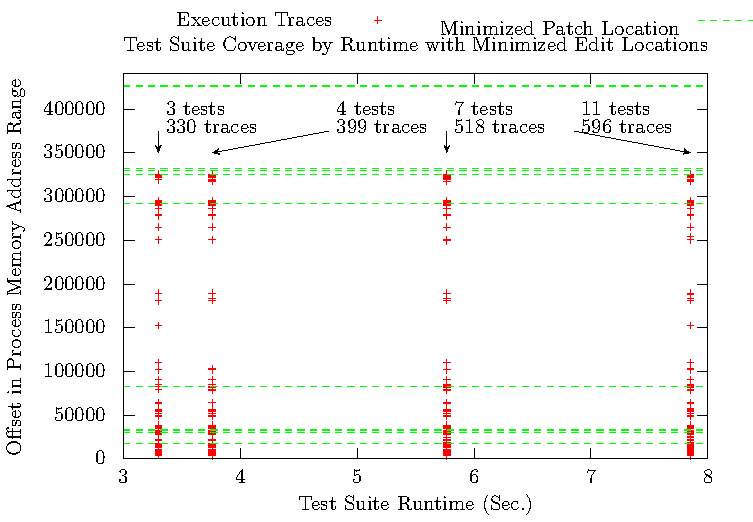
\includegraphics[width=0.46\textwidth]{ts-cov-and-runtime-w-min.pdf}  
  \caption{Test suite coverage shown by runtime.  The location of
    minimized edits in successful repairs are shown as well.  Every
    successful edit included a repair which was not located on the
    test suite trace.}
  \label{ts-cov-rt-w-min}
\end{figure}

In 8 of the 10 attempted repairs only the three exploit tests were
used with no regression tests run.  This corresponds to the first
group of traces labeled ``3 tests'' in Figure \ref{ts-cov-rt-w-min}.

In these cases the repair process averaged ~36,000 total fitness
evaluations taking on average 86.6 minutes to find a repair using 32
virtual machines for parallelized fitness evaluation.

\subsubsection{No Fault Localization}
\label{no-fault-localization}

In addition to adding an extra and sometimes burdensome step to the
application of evolutionary program repair, the use of fault
localization has the more serious problem of sometimes
over-constraining the mutation operations eliminating the possibility
of finding valid repairs.

One of the NETGEAR exploits falls into the later case in which fault
localization prevents the repair process from succeeding.  As shown in
Figure \ref{ts-cov-rt-w-min}; many of the places where successful
repairs changed the program were no located on the trace information.
In fact, only 2 of the 22 program locations modified by repairs found
in this work were within 3 instructions of the execution traces.

Previous techniques of evolutionary program repair which confine edit
operations to execution traces are likely unable to repair some
programs for this reason.
% FIXME Wes:
% Do you agree with this statement?  Another way to state this is that
% regular genprog will never mutate some relevant portions of the
% program program, e.g., data such as structs which can not be labeled
% using execution traces.

\subsubsection{Minimization Impact}
\label{minimization}

In some cases the initial evolved repair was not satisfactory.  For
example, evolved repairs sometimes worked when \texttt{net-cgi} was
called directly on the command line but not through the embedded
$\mu$HTTPd webserver,\footnote{\url{http://wiki.openwrt.org/doc/uci/uhttpd}}
or the evolved file failed to serve pages not used in the
exploit test.  As shown in Table \ref{minimized-stats}, however, in most
cases the minimized version of the evolved executable was satisfactory
and passed all hand-written regression tests available, even those not used
during the repair process. 

\begin{table}[htb]
\centering
\begin{tabular}{rrrrrr}
Run  & Fit Evals & Full Diff & Min Diff & Full Fit & Min Fit \\
\toprule
0    & 90405     & 500       & 2        & 8        & 22      \\
1    & 17231     & 134       & 3        & 22       & 22      \\
2    & 26879     & 205       & 2        & 21       & 22      \\
3    & 23764     & 199       & 2        & 19       & 22      \\
4    & 47906     & 319       & 2        & 6        & 6       \\
5    & 13102     & 95        & 2        & 16       & 22      \\
6    & 76960     & 556       & 3        & 17       & 22      \\
7    & 11831     & 79        & 3        & 20       & 22      \\
8    & 2846      & 10        & 1        & 14       & 14      \\
9    & 25600     & 182       & 2        & 21       & 22      \\
\bottomrule
mean & 33652.4   & 227.9     & 2.2      & 16.4     & 19.6    \\
\end{tabular}
\caption{\label{minimized-stats}Difference and functionality of
evolved repair before and after minimization.  In these columns ``Full''
refers to evolved solutions before minimization and ``Min'' refers to
post-minimization solutions.  Columns labeled ``Diff'' report the number
of unified diff windows against the original program data. The columns
labeled ``Fit'' report the fitness measured with a full regression test
suite including the exploit tests with a maximum fitness of 22.}
\end{table}

As shown in Table \ref{minimized-stats}, the initial evolved repair
differed from the original at over 200 locations on average in the ELF
program data, while the minimized repairs differed at only 1--3
locations on average.  This great discrepancy is due to the
accumulation of candidate edits in non-tested portions of the program
data.  Since these portions of the genome were not tested, there was
no evolutionary pressure to purge harmful edits.  The elimination of
these accumulated edits is the main purpose of our minimization step,
and is the reason for the consistent increase in regression test
behavior found in the minimized repairs.

\subsubsection{Iterative Repair}
\label{iterative-repair}
These repairs required two distinct fixes addressing two different
exploits in a single evolutionary run.  This is an instance of
``iterative repair'' which has not previously been observed in the
repair of real-world extant software.

% \begin{figure}[htb]
%   \centering
%   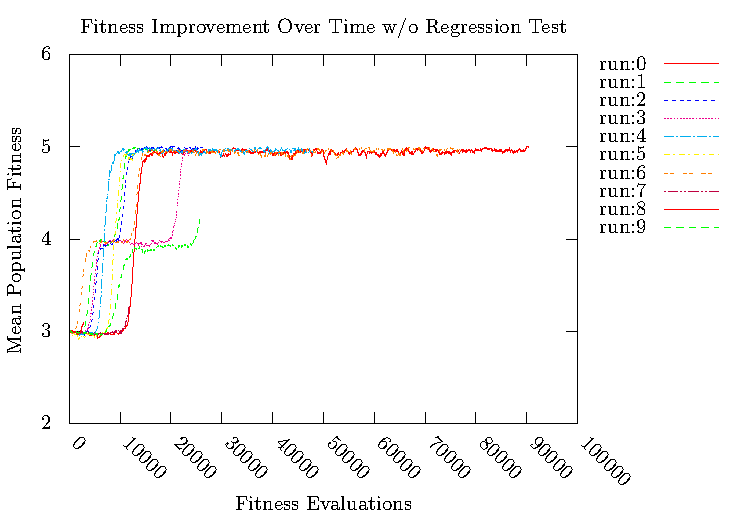
\includegraphics[bb=0 0 355 248,width=0.46\textwidth]{fitness-improvement.pdf}
%   % 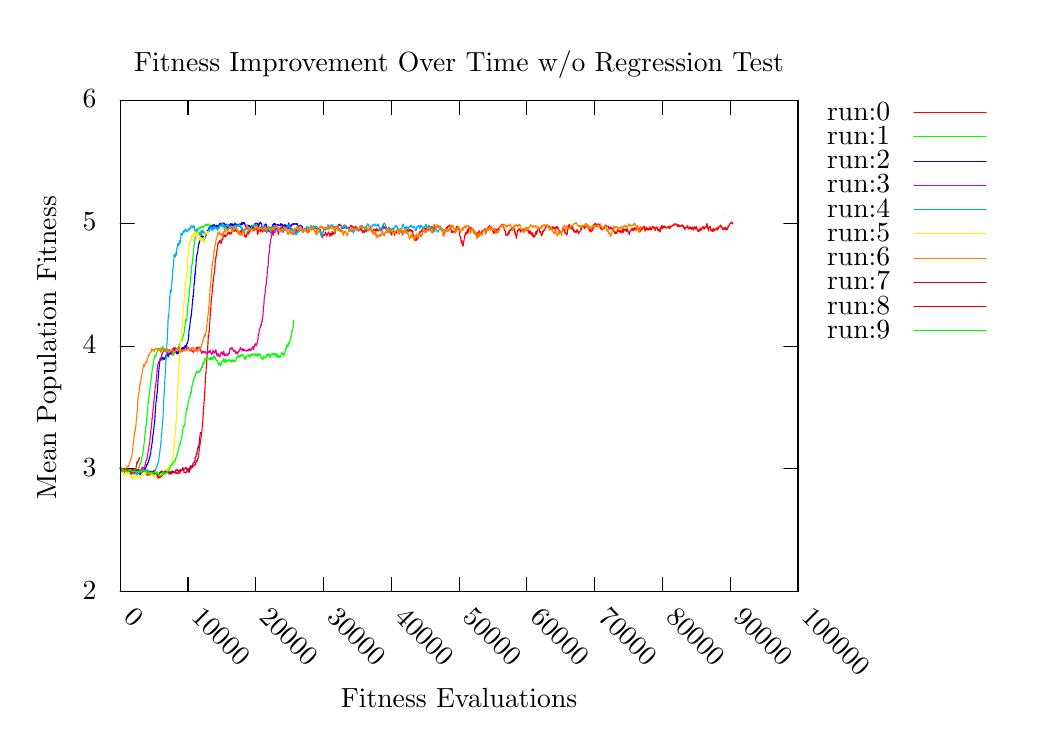
\begin{tikzpicture}[gnuplot]
%% generated with GNUPLOT 4.7p0 (Lua 5.2; terminal rev. 99, script rev. 100)
%% Tue 26 Nov 2013 03:16:23 PM MST
\path (0.000,0.000) rectangle (12.500,8.750);
\gpcolor{color=gp lt color border}
\gpsetlinetype{gp lt border}
\gpsetlinewidth{1.00}
\draw[gp path] (1.136,1.587)--(1.316,1.587);
\draw[gp path] (9.743,1.587)--(9.563,1.587);
\node[gp node right] at (0.952,1.587) { 2};
\draw[gp path] (1.136,3.147)--(1.316,3.147);
\draw[gp path] (9.743,3.147)--(9.563,3.147);
\node[gp node right] at (0.952,3.147) { 3};
\draw[gp path] (1.136,4.706)--(1.316,4.706);
\draw[gp path] (9.743,4.706)--(9.563,4.706);
\node[gp node right] at (0.952,4.706) { 4};
\draw[gp path] (1.136,6.266)--(1.316,6.266);
\draw[gp path] (9.743,6.266)--(9.563,6.266);
\node[gp node right] at (0.952,6.266) { 5};
\draw[gp path] (1.136,7.825)--(1.316,7.825);
\draw[gp path] (9.743,7.825)--(9.563,7.825);
\node[gp node right] at (0.952,7.825) { 6};
\draw[gp path] (1.136,1.587)--(1.136,1.767);
\draw[gp path] (1.136,7.825)--(1.136,7.645);
\node[gp node left,rotate=-45] at (1.136,1.403) { 0};
\draw[gp path] (1.997,1.587)--(1.997,1.767);
\draw[gp path] (1.997,7.825)--(1.997,7.645);
\node[gp node left,rotate=-45] at (1.997,1.403) { 10000};
\draw[gp path] (2.857,1.587)--(2.857,1.767);
\draw[gp path] (2.857,7.825)--(2.857,7.645);
\node[gp node left,rotate=-45] at (2.857,1.403) { 20000};
\draw[gp path] (3.718,1.587)--(3.718,1.767);
\draw[gp path] (3.718,7.825)--(3.718,7.645);
\node[gp node left,rotate=-45] at (3.718,1.403) { 30000};
\draw[gp path] (4.579,1.587)--(4.579,1.767);
\draw[gp path] (4.579,7.825)--(4.579,7.645);
\node[gp node left,rotate=-45] at (4.579,1.403) { 40000};
\draw[gp path] (5.440,1.587)--(5.440,1.767);
\draw[gp path] (5.440,7.825)--(5.440,7.645);
\node[gp node left,rotate=-45] at (5.440,1.403) { 50000};
\draw[gp path] (6.300,1.587)--(6.300,1.767);
\draw[gp path] (6.300,7.825)--(6.300,7.645);
\node[gp node left,rotate=-45] at (6.300,1.403) { 60000};
\draw[gp path] (7.161,1.587)--(7.161,1.767);
\draw[gp path] (7.161,7.825)--(7.161,7.645);
\node[gp node left,rotate=-45] at (7.161,1.403) { 70000};
\draw[gp path] (8.022,1.587)--(8.022,1.767);
\draw[gp path] (8.022,7.825)--(8.022,7.645);
\node[gp node left,rotate=-45] at (8.022,1.403) { 80000};
\draw[gp path] (8.882,1.587)--(8.882,1.767);
\draw[gp path] (8.882,7.825)--(8.882,7.645);
\node[gp node left,rotate=-45] at (8.882,1.403) { 90000};
\draw[gp path] (9.743,1.587)--(9.743,1.767);
\draw[gp path] (9.743,7.825)--(9.743,7.645);
\node[gp node left,rotate=-45] at (9.743,1.403) { 100000};
\draw[gp path] (1.136,7.825)--(1.136,1.587)--(9.743,1.587)--(9.743,7.825)--cycle;
\node[gp node center,rotate=-270] at (0.246,4.706) {Mean Population Fitness};
\node[gp node center] at (5.439,0.215) {Fitness Evaluations};
\node[gp node center] at (5.439,8.287) {Fitness Improvement Over Time w/o Regression Test};
\node[gp node right] at (11.031,7.671) {run:0};
\gpcolor{color=gp lt color 0}
\gpsetlinetype{gp lt plot 0}
\draw[gp path] (11.215,7.671)--(12.131,7.671);
\draw[gp path] (1.137,3.147)--(1.139,3.165)--(1.140,3.164)--(1.142,3.163)--(1.143,3.162)%
  --(1.144,3.162)--(1.146,3.161)--(1.147,3.161)--(1.148,3.161)--(1.150,3.156)--(1.151,3.156)%
  --(1.153,3.155)--(1.154,3.155)--(1.155,3.155)--(1.158,3.154)--(1.159,3.150)--(1.161,3.150)%
  --(1.162,3.150)--(1.164,3.150)--(1.165,3.150)--(1.166,3.147)--(1.168,3.147)--(1.169,3.147)%
  --(1.171,3.147)--(1.172,3.147)--(1.173,3.147)--(1.175,3.147)--(1.176,3.147)--(1.177,3.147)%
  --(1.179,3.150)--(1.180,3.150)--(1.181,3.147)--(1.183,3.150)--(1.184,3.143)--(1.186,3.143)%
  --(1.187,3.143)--(1.188,3.143)--(1.190,3.143)--(1.191,3.140)--(1.193,3.140)--(1.194,3.140)%
  --(1.195,3.134)--(1.197,3.134)--(1.198,3.134)--(1.199,3.131)--(1.201,3.125)--(1.202,3.128)%
  --(1.203,3.125)--(1.205,3.125)--(1.206,3.125)--(1.208,3.125)--(1.209,3.116)--(1.210,3.116)%
  --(1.212,3.116)--(1.213,3.110)--(1.214,3.110)--(1.216,3.110)--(1.217,3.110)--(1.219,3.110)%
  --(1.220,3.116)--(1.221,3.116)--(1.223,3.116)--(1.224,3.125)--(1.226,3.125)--(1.227,3.125)%
  --(1.233,3.137)--(1.234,3.134)--(1.235,3.134)--(1.237,3.137)--(1.238,3.131)--(1.239,3.128)%
  --(1.241,3.128)--(1.242,3.128)--(1.243,3.125)--(1.245,3.122)--(1.246,3.122)--(1.248,3.122)%
  --(1.249,3.116)--(1.250,3.125)--(1.252,3.125)--(1.253,3.128)--(1.254,3.128)--(1.256,3.125)%
  --(1.257,3.131)--(1.259,3.131)--(1.260,3.131)--(1.261,3.131)--(1.263,3.131)--(1.264,3.131)%
  --(1.265,3.125)--(1.267,3.125)--(1.268,3.122)--(1.270,3.122)--(1.271,3.122)--(1.272,3.122)%
  --(1.274,3.122)--(1.275,3.119)--(1.276,3.113)--(1.278,3.110)--(1.279,3.116)--(1.281,3.110)%
  --(1.282,3.113)--(1.283,3.113)--(1.285,3.113)--(1.286,3.113)--(1.287,3.116)--(1.289,3.113)%
  --(1.290,3.113)--(1.292,3.116)--(1.293,3.116)--(1.294,3.119)--(1.296,3.113)--(1.297,3.113)%
  --(1.299,3.110)--(1.300,3.110)--(1.301,3.110)--(1.303,3.104)--(1.304,3.116)--(1.305,3.113)%
  --(1.307,3.113)--(1.308,3.113)--(1.310,3.113)--(1.311,3.113)--(1.312,3.113)--(1.314,3.116)%
  --(1.315,3.116)--(1.316,3.116)--(1.318,3.122)--(1.319,3.125)--(1.321,3.122)--(1.322,3.122)%
  --(1.323,3.107)--(1.325,3.110)--(1.326,3.116)--(1.327,3.116)--(1.329,3.116)--(1.330,3.116)%
  --(1.332,3.113)--(1.333,3.113)--(1.334,3.113)--(1.336,3.107)--(1.337,3.101)--(1.338,3.110)%
  --(1.340,3.110)--(1.341,3.113)--(1.343,3.113)--(1.344,3.113)--(1.345,3.113)--(1.347,3.113)%
  --(1.348,3.116)--(1.349,3.116)--(1.351,3.116)--(1.352,3.119)--(1.354,3.122)--(1.355,3.113)%
  --(1.356,3.113)--(1.358,3.113)--(1.359,3.113)--(1.360,3.110)--(1.362,3.110)--(1.363,3.110)%
  --(1.365,3.110)--(1.366,3.116)--(1.367,3.110)--(1.369,3.110)--(1.370,3.104)--(1.371,3.101)%
  --(1.373,3.107)--(1.374,3.104)--(1.376,3.110)--(1.377,3.110)--(1.379,3.110)--(1.380,3.110)%
  --(1.381,3.107)--(1.383,3.107)--(1.384,3.104)--(1.385,3.107)--(1.387,3.110)--(1.388,3.110)%
  --(1.389,3.110)--(1.391,3.113)--(1.392,3.113)--(1.394,3.113)--(1.395,3.113)--(1.396,3.113)%
  --(1.398,3.104)--(1.399,3.107)--(1.401,3.104)--(1.402,3.104)--(1.403,3.107)--(1.405,3.104)%
  --(1.406,3.098)--(1.407,3.101)--(1.409,3.110)--(1.410,3.116)--(1.411,3.116)--(1.413,3.116)%
  --(1.414,3.122)--(1.416,3.116)--(1.417,3.116)--(1.418,3.116)--(1.420,3.116)--(1.421,3.116)%
  --(1.422,3.119)--(1.424,3.119)--(1.425,3.119)--(1.427,3.119)--(1.428,3.119)--(1.429,3.113)%
  --(1.431,3.116)--(1.432,3.116)--(1.433,3.113)--(1.435,3.113)--(1.436,3.110)--(1.438,3.110)%
  --(1.439,3.116)--(1.440,3.110)--(1.442,3.107)--(1.443,3.107)--(1.444,3.107)--(1.446,3.104)%
  --(1.447,3.101)--(1.449,3.101)--(1.450,3.098)--(1.451,3.098)--(1.453,3.092)--(1.454,3.092)%
  --(1.455,3.092)--(1.457,3.092)--(1.458,3.089)--(1.460,3.089)--(1.461,3.089)--(1.462,3.092)%
  --(1.464,3.092)--(1.465,3.098)--(1.467,3.098)--(1.468,3.098)--(1.469,3.092)--(1.471,3.085)%
  --(1.472,3.070)--(1.474,3.079)--(1.475,3.076)--(1.476,3.067)--(1.478,3.067)--(1.479,3.067)%
  --(1.480,3.067)--(1.482,3.067)--(1.483,3.067)--(1.484,3.067)--(1.486,3.067)--(1.487,3.070)%
  --(1.489,3.067)--(1.490,3.082)--(1.491,3.082)--(1.493,3.079)--(1.494,3.076)--(1.495,3.079)%
  --(1.497,3.076)--(1.498,3.082)--(1.500,3.079)--(1.501,3.073)--(1.502,3.076)--(1.504,3.070)%
  --(1.505,3.067)--(1.506,3.076)--(1.508,3.076)--(1.509,3.076)--(1.511,3.076)--(1.512,3.076)%
  --(1.513,3.085)--(1.515,3.085)--(1.516,3.082)--(1.517,3.085)--(1.519,3.089)--(1.520,3.085)%
  --(1.522,3.089)--(1.523,3.079)--(1.524,3.085)--(1.526,3.085)--(1.527,3.085)--(1.528,3.085)%
  --(1.530,3.092)--(1.531,3.101)--(1.533,3.095)--(1.534,3.085)--(1.536,3.086)--(1.537,3.092)%
  --(1.538,3.079)--(1.539,3.079)--(1.541,3.079)--(1.542,3.079)--(1.544,3.082)--(1.545,3.089)%
  --(1.546,3.089)--(1.548,3.082)--(1.549,3.079)--(1.551,3.079)--(1.552,3.076)--(1.553,3.073)%
  --(1.555,3.073)--(1.556,3.073)--(1.557,3.073)--(1.559,3.073)--(1.560,3.073)--(1.562,3.073)%
  --(1.563,3.070)--(1.564,3.070)--(1.566,3.070)--(1.567,3.085)--(1.568,3.082)--(1.570,3.095)%
  --(1.571,3.089)--(1.573,3.085)--(1.574,3.085)--(1.575,3.089)--(1.577,3.089)--(1.578,3.089)%
  --(1.579,3.089)--(1.581,3.092)--(1.582,3.095)--(1.584,3.101)--(1.585,3.101)--(1.586,3.101)%
  --(1.588,3.101)--(1.589,3.101)--(1.590,3.098)--(1.592,3.095)--(1.593,3.095)--(1.595,3.092)%
  --(1.596,3.085)--(1.597,3.079)--(1.599,3.082)--(1.600,3.082)--(1.601,3.076)--(1.603,3.076)%
  --(1.604,3.076)--(1.606,3.064)--(1.607,3.058)--(1.609,3.055)--(1.610,3.049)--(1.611,3.043)%
  --(1.612,3.040)--(1.614,3.031)--(1.615,3.024)--(1.617,3.027)--(1.618,3.034)--(1.619,3.034)%
  --(1.621,3.040)--(1.622,3.040)--(1.624,3.046)--(1.625,3.049)--(1.626,3.043)--(1.628,3.043)%
  --(1.629,3.037)--(1.630,3.040)--(1.632,3.043)--(1.633,3.046)--(1.635,3.043)--(1.636,3.046)%
  --(1.637,3.046)--(1.639,3.043)--(1.640,3.037)--(1.641,3.049)--(1.643,3.049)--(1.644,3.046)%
  --(1.646,3.040)--(1.647,3.040)--(1.648,3.043)--(1.650,3.049)--(1.651,3.049)--(1.653,3.046)%
  --(1.654,3.052)--(1.655,3.052)--(1.657,3.046)--(1.658,3.052)--(1.659,3.055)--(1.661,3.055)%
  --(1.662,3.055)--(1.664,3.058)--(1.665,3.061)--(1.666,3.061)--(1.668,3.064)--(1.669,3.061)%
  --(1.670,3.058)--(1.672,3.067)--(1.673,3.067)--(1.674,3.067)--(1.676,3.076)--(1.677,3.073)%
  --(1.679,3.070)--(1.680,3.070)--(1.681,3.070)--(1.683,3.079)--(1.684,3.092)--(1.685,3.092)%
  --(1.687,3.092)--(1.688,3.089)--(1.690,3.092)--(1.691,3.092)--(1.693,3.085)--(1.694,3.095)%
  --(1.695,3.098)--(1.696,3.098)--(1.698,3.098)--(1.699,3.092)--(1.701,3.085)--(1.702,3.089)%
  --(1.703,3.101)--(1.705,3.101)--(1.706,3.110)--(1.708,3.107)--(1.709,3.107)--(1.710,3.107)%
  --(1.712,3.107)--(1.713,3.107)--(1.714,3.110)--(1.716,3.101)--(1.717,3.098)--(1.719,3.104)%
  --(1.720,3.104)--(1.721,3.110)--(1.723,3.110)--(1.724,3.110)--(1.725,3.110)--(1.727,3.110)%
  --(1.728,3.113)--(1.730,3.113)--(1.731,3.113)--(1.732,3.116)--(1.734,3.116)--(1.735,3.116)%
  --(1.736,3.110)--(1.738,3.110)--(1.739,3.110)--(1.741,3.107)--(1.742,3.113)--(1.743,3.113)%
  --(1.745,3.113)--(1.746,3.113)--(1.747,3.110)--(1.749,3.110)--(1.750,3.110)--(1.752,3.107)%
  --(1.753,3.101)--(1.754,3.098)--(1.756,3.098)--(1.757,3.098)--(1.758,3.095)--(1.760,3.092)%
  --(1.761,3.104)--(1.763,3.101)--(1.764,3.101)--(1.765,3.101)--(1.767,3.098)--(1.768,3.101)%
  --(1.769,3.101)--(1.771,3.101)--(1.772,3.101)--(1.774,3.101)--(1.775,3.107)--(1.776,3.104)%
  --(1.778,3.107)--(1.779,3.116)--(1.780,3.116)--(1.782,3.116)--(1.783,3.116)--(1.785,3.116)%
  --(1.786,3.116)--(1.787,3.116)--(1.789,3.116)--(1.790,3.116)--(1.792,3.116)--(1.793,3.119)%
  --(1.794,3.119)--(1.796,3.119)--(1.797,3.119)--(1.798,3.122)--(1.800,3.116)--(1.801,3.116)%
  --(1.803,3.116)--(1.804,3.116)--(1.805,3.113)--(1.807,3.113)--(1.808,3.113)--(1.809,3.113)%
  --(1.811,3.110)--(1.812,3.110)--(1.814,3.110)--(1.815,3.110)--(1.816,3.107)--(1.818,3.107)%
  --(1.819,3.104)--(1.820,3.104)--(1.822,3.104)--(1.823,3.107)--(1.825,3.104)--(1.826,3.104)%
  --(1.827,3.104)--(1.829,3.104)--(1.830,3.095)--(1.831,3.095)--(1.833,3.092)--(1.834,3.095)%
  --(1.836,3.098)--(1.837,3.092)--(1.838,3.098)--(1.840,3.098)--(1.841,3.098)--(1.842,3.101)%
  --(1.844,3.098)--(1.845,3.098)--(1.847,3.098)--(1.848,3.095)--(1.849,3.089)--(1.851,3.089)%
  --(1.852,3.085)--(1.854,3.086)--(1.855,3.092)--(1.856,3.092)--(1.858,3.098)--(1.859,3.098)%
  --(1.860,3.092)--(1.862,3.095)--(1.863,3.092)--(1.864,3.089)--(1.866,3.085)--(1.867,3.089)%
  --(1.869,3.089)--(1.870,3.092)--(1.871,3.095)--(1.873,3.092)--(1.874,3.089)--(1.876,3.092)%
  --(1.877,3.092)--(1.878,3.098)--(1.880,3.101)--(1.881,3.101)--(1.882,3.098)--(1.884,3.098)%
  --(1.885,3.098)--(1.887,3.098)--(1.888,3.101)--(1.889,3.092)--(1.891,3.098)--(1.892,3.098)%
  --(1.893,3.098)--(1.895,3.098)--(1.896,3.098)--(1.898,3.110)--(1.899,3.116)--(1.900,3.113)%
  --(1.902,3.113)--(1.903,3.119)--(1.904,3.119)--(1.906,3.116)--(1.907,3.116)--(1.909,3.125)%
  --(1.910,3.125)--(1.911,3.125)--(1.913,3.125)--(1.914,3.125)--(1.916,3.125)--(1.917,3.128)%
  --(1.918,3.128)--(1.920,3.128)--(1.921,3.131)--(1.922,3.131)--(1.924,3.134)--(1.925,3.131)%
  --(1.927,3.131)--(1.928,3.131)--(1.929,3.131)--(1.931,3.131)--(1.932,3.131)--(1.933,3.131)%
  --(1.935,3.131)--(1.936,3.131)--(1.938,3.131)--(1.939,3.137)--(1.940,3.134)--(1.942,3.131)%
  --(1.943,3.125)--(1.944,3.113)--(1.946,3.101)--(1.947,3.101)--(1.949,3.104)--(1.950,3.107)%
  --(1.951,3.101)--(1.953,3.101)--(1.954,3.104)--(1.955,3.104)--(1.957,3.104)--(1.958,3.101)%
  --(1.960,3.101)--(1.961,3.101)--(1.962,3.098)--(1.964,3.098)--(1.965,3.098)--(1.966,3.098)%
  --(1.968,3.104)--(1.969,3.104)--(1.971,3.098)--(1.972,3.098)--(1.973,3.098)--(1.975,3.104)%
  --(1.976,3.101)--(1.977,3.101)--(1.979,3.101)--(1.980,3.116)--(1.982,3.119)--(1.983,3.125)%
  --(1.984,3.125)--(1.986,3.128)--(1.987,3.131)--(1.988,3.131)--(1.990,3.131)--(1.991,3.125)%
  --(1.993,3.125)--(1.994,3.131)--(1.995,3.128)--(1.997,3.137)--(1.998,3.131)--(1.999,3.131)%
  --(2.001,3.146)--(2.002,3.150)--(2.004,3.147)--(2.005,3.147)--(2.006,3.140)--(2.008,3.143)%
  --(2.009,3.150)--(2.010,3.150)--(2.012,3.159)--(2.013,3.156)--(2.015,3.156)--(2.016,3.156)%
  --(2.017,3.156)--(2.019,3.156)--(2.020,3.150)--(2.021,3.143)--(2.023,3.143)--(2.024,3.150)%
  --(2.026,3.150)--(2.027,3.150)--(2.028,3.137)--(2.030,3.143)--(2.031,3.156)--(2.033,3.159)%
  --(2.034,3.150)--(2.035,3.156)--(2.037,3.159)--(2.038,3.162)--(2.039,3.162)--(2.041,3.162)%
  --(2.042,3.162)--(2.044,3.162)--(2.045,3.165)--(2.046,3.165)--(2.048,3.165)--(2.049,3.165)%
  --(2.050,3.168)--(2.052,3.165)--(2.053,3.171)--(2.055,3.174)--(2.056,3.174)--(2.057,3.180)%
  --(2.059,3.171)--(2.060,3.171)--(2.061,3.186)--(2.063,3.186)--(2.064,3.186)--(2.066,3.186)%
  --(2.067,3.186)--(2.068,3.192)--(2.070,3.189)--(2.071,3.195)--(2.072,3.195)--(2.074,3.189)%
  --(2.075,3.189)--(2.077,3.189)--(2.078,3.189)--(2.082,3.201)--(2.083,3.201)--(2.085,3.195)%
  --(2.086,3.201)--(2.088,3.201)--(2.089,3.201)--(2.090,3.201)--(2.092,3.201)--(2.093,3.204)%
  --(2.094,3.214)--(2.096,3.226)--(2.097,3.232)--(2.099,3.232)--(2.100,3.232)--(2.101,3.232)%
  --(2.103,3.238)--(2.104,3.244)--(2.105,3.250)--(2.107,3.244)--(2.108,3.241)--(2.110,3.238)%
  --(2.111,3.244)--(2.112,3.250)--(2.114,3.250)--(2.115,3.259)--(2.117,3.256)--(2.118,3.262)%
  --(2.119,3.266)--(2.121,3.278)--(2.122,3.275)--(2.123,3.287)--(2.125,3.284)--(2.126,3.284)%
  --(2.128,3.284)--(2.129,3.302)--(2.130,3.308)--(2.132,3.323)--(2.133,3.333)--(2.134,3.345)%
  --(2.136,3.366)--(2.137,3.372)--(2.139,3.385)--(2.140,3.391)--(2.141,3.418)--(2.143,3.430)%
  --(2.144,3.436)--(2.145,3.443)--(2.147,3.449)--(2.148,3.449)--(2.150,3.455)--(2.151,3.464)%
  --(2.152,3.473)--(2.154,3.494)--(2.155,3.494)--(2.156,3.497)--(2.158,3.516)--(2.159,3.516)%
  --(2.161,3.537)--(2.162,3.537)--(2.163,3.546)--(2.165,3.562)--(2.166,3.577)--(2.167,3.592)%
  --(2.169,3.592)--(2.170,3.604)--(2.172,3.616)--(2.173,3.635)--(2.174,3.635)--(2.176,3.650)%
  --(2.177,3.681)--(2.179,3.687)--(2.180,3.702)--(2.181,3.732)--(2.183,3.732)--(2.184,3.748)%
  --(2.185,3.781)--(2.187,3.787)--(2.188,3.824)--(2.190,3.833)--(2.191,3.864)--(2.192,3.888)%
  --(2.194,3.916)--(2.195,3.922)--(2.196,3.934)--(2.198,3.952)--(2.199,3.974)--(2.201,4.001)%
  --(2.202,4.007)--(2.203,4.022)--(2.205,4.056)--(2.206,4.074)--(2.207,4.093)--(2.209,4.117)%
  --(2.210,4.141)--(2.212,4.154)--(2.213,4.184)--(2.214,4.224)--(2.216,4.254)--(2.217,4.288)%
  --(2.219,4.306)--(2.220,4.331)--(2.221,4.355)--(2.223,4.355)--(2.224,4.355)--(2.225,4.364)%
  --(2.227,4.401)--(2.228,4.434)--(2.230,4.444)--(2.231,4.468)--(2.232,4.501)--(2.234,4.520)%
  --(2.235,4.520)--(2.236,4.532)--(2.238,4.553)--(2.239,4.587)--(2.240,4.596)--(2.242,4.608)%
  --(2.243,4.621)--(2.245,4.663)--(2.246,4.685)--(2.247,4.694)--(2.249,4.721)--(2.250,4.733)%
  --(2.251,4.764)--(2.253,4.797)--(2.254,4.825)--(2.256,4.831)--(2.257,4.846)--(2.258,4.834)%
  --(2.260,4.843)--(2.261,4.852)--(2.263,4.880)--(2.264,4.895)--(2.265,4.895)--(2.267,4.898)%
  --(2.268,4.932)--(2.269,4.990)--(2.271,4.996)--(2.272,4.996)--(2.274,5.008)--(2.275,5.039)%
  --(2.276,5.057)--(2.278,5.084)--(2.279,5.100)--(2.280,5.118)--(2.282,5.136)--(2.283,5.145)%
  --(2.285,5.158)--(2.286,5.191)--(2.287,5.216)--(2.289,5.240)--(2.290,5.255)--(2.291,5.277)%
  --(2.293,5.280)--(2.294,5.304)--(2.296,5.313)--(2.297,5.329)--(2.298,5.332)--(2.300,5.347)%
  --(2.301,5.362)--(2.302,5.365)--(2.304,5.390)--(2.305,5.423)--(2.307,5.441)--(2.308,5.435)%
  --(2.309,5.454)--(2.311,5.472)--(2.312,5.490)--(2.314,5.506)--(2.315,5.515)--(2.316,5.519)%
  --(2.318,5.548)--(2.319,5.564)--(2.320,5.564)--(2.322,5.570)--(2.323,5.594)--(2.324,5.591)%
  --(2.326,5.622)--(2.327,5.615)--(2.329,5.623)--(2.330,5.637)--(2.331,5.637)--(2.333,5.649)%
  --(2.334,5.646)--(2.335,5.679)--(2.337,5.698)--(2.338,5.692)--(2.340,5.734)--(2.341,5.762)%
  --(2.342,5.780)--(2.344,5.771)--(2.345,5.786)--(2.346,5.789)--(2.348,5.811)--(2.349,5.829)%
  --(2.351,5.814)--(2.352,5.823)--(2.353,5.850)--(2.355,5.863)--(2.356,5.854)--(2.358,5.863)%
  --(2.359,5.878)--(2.360,5.884)--(2.362,5.902)--(2.363,5.921)--(2.364,5.918)--(2.366,5.921)%
  --(2.367,5.930)--(2.369,5.942)--(2.370,5.948)--(2.371,5.936)--(2.373,5.957)--(2.374,5.985)%
  --(2.375,5.997)--(2.377,5.997)--(2.378,6.015)--(2.380,6.012)--(2.381,6.015)--(2.382,6.009)%
  --(2.384,6.012)--(2.385,6.021)--(2.386,6.021)--(2.388,6.021)--(2.389,6.015)--(2.391,6.021)%
  --(2.392,6.027)--(2.393,6.034)--(2.395,6.031)--(2.396,6.034)--(2.397,6.040)--(2.399,6.034)%
  --(2.400,6.024)--(2.402,6.030)--(2.403,6.052)--(2.404,6.052)--(2.406,6.046)--(2.407,6.049)%
  --(2.408,6.046)--(2.410,6.031)--(2.411,6.024)--(2.413,6.024)--(2.414,6.030)--(2.415,6.009)%
  --(2.417,6.009)--(2.418,6.015)--(2.419,6.012)--(2.421,6.027)--(2.422,6.043)--(2.424,6.043)%
  --(2.425,6.043)--(2.426,6.055)--(2.428,6.067)--(2.429,6.070)--(2.430,6.073)--(2.432,6.079)%
  --(2.433,6.061)--(2.435,6.058)--(2.436,6.058)--(2.437,6.061)--(2.439,6.064)--(2.440,6.082)%
  --(2.442,6.085)--(2.443,6.104)--(2.444,6.107)--(2.446,6.113)--(2.447,6.113)--(2.448,6.110)%
  --(2.450,6.110)--(2.451,6.113)--(2.453,6.107)--(2.454,6.116)--(2.455,6.116)--(2.457,6.116)%
  --(2.458,6.104)--(2.459,6.104)--(2.461,6.098)--(2.462,6.095)--(2.464,6.107)--(2.465,6.119)%
  --(2.466,6.101)--(2.468,6.092)--(2.469,6.110)--(2.470,6.119)--(2.472,6.119)--(2.473,6.104)%
  --(2.475,6.098)--(2.476,6.110)--(2.477,6.110)--(2.479,6.110)--(2.480,6.113)--(2.481,6.116)%
  --(2.483,6.113)--(2.484,6.113)--(2.486,6.110)--(2.487,6.113)--(2.488,6.110)--(2.490,6.110)%
  --(2.491,6.110)--(2.492,6.110)--(2.494,6.119)--(2.495,6.125)--(2.497,6.131)--(2.498,6.134)%
  --(2.499,6.128)--(2.501,6.137)--(2.502,6.140)--(2.503,6.140)--(2.505,6.156)--(2.506,6.153)%
  --(2.508,6.156)--(2.509,6.156)--(2.510,6.137)--(2.512,6.137)--(2.513,6.140)--(2.514,6.140)%
  --(2.516,6.140)--(2.517,6.137)--(2.519,6.131)--(2.520,6.137)--(2.521,6.131)--(2.523,6.153)%
  --(2.524,6.131)--(2.526,6.128)--(2.527,6.128)--(2.528,6.128)--(2.530,6.128)--(2.531,6.137)%
  --(2.532,6.140)--(2.534,6.137)--(2.535,6.137)--(2.537,6.140)--(2.538,6.137)--(2.539,6.140)%
  --(2.541,6.143)--(2.542,6.137)--(2.543,6.137)--(2.545,6.128)--(2.546,6.156)--(2.548,6.156)%
  --(2.549,6.174)--(2.550,6.174)--(2.552,6.156)--(2.553,6.159)--(2.555,6.159)--(2.556,6.171)%
  --(2.557,6.162)--(2.559,6.174)--(2.560,6.180)--(2.561,6.198)--(2.563,6.186)--(2.564,6.183)%
  --(2.565,6.192)--(2.567,6.192)--(2.568,6.192)--(2.570,6.195)--(2.571,6.192)--(2.572,6.189)%
  --(2.574,6.183)--(2.575,6.192)--(2.576,6.180)--(2.578,6.177)--(2.579,6.168)--(2.581,6.168)%
  --(2.582,6.162)--(2.583,6.171)--(2.585,6.168)--(2.586,6.177)--(2.587,6.177)--(2.589,6.177)%
  --(2.590,6.177)--(2.592,6.177)--(2.593,6.180)--(2.594,6.171)--(2.596,6.171)--(2.597,6.177)%
  --(2.599,6.177)--(2.600,6.183)--(2.601,6.180)--(2.603,6.171)--(2.604,6.177)--(2.605,6.201)%
  --(2.607,6.195)--(2.608,6.186)--(2.610,6.180)--(2.611,6.168)--(2.612,6.165)--(2.614,6.162)%
  --(2.615,6.162)--(2.616,6.159)--(2.618,6.159)--(2.619,6.162)--(2.621,6.156)--(2.622,6.159)%
  --(2.623,6.162)--(2.625,6.165)--(2.626,6.165)--(2.627,6.159)--(2.629,6.156)--(2.630,6.146)%
  --(2.632,6.156)--(2.633,6.156)--(2.634,6.143)--(2.636,6.140)--(2.637,6.134)--(2.638,6.131)%
  --(2.640,6.137)--(2.641,6.134)--(2.643,6.140)--(2.644,6.140)--(2.645,6.131)--(2.647,6.128)%
  --(2.648,6.122)--(2.649,6.122)--(2.651,6.131)--(2.652,6.149)--(2.654,6.156)--(2.655,6.156)%
  --(2.656,6.153)--(2.658,6.165)--(2.659,6.162)--(2.660,6.168)--(2.662,6.165)--(2.663,6.168)%
  --(2.665,6.165)--(2.666,6.174)--(2.667,6.171)--(2.669,6.174)--(2.671,6.177)--(2.673,6.165)%
  --(2.674,6.165)--(2.676,6.159)--(2.677,6.146)--(2.678,6.153)--(2.680,6.156)--(2.681,6.150)%
  --(2.683,6.159)--(2.684,6.165)--(2.685,6.159)--(2.687,6.162)--(2.688,6.150)--(2.689,6.159)%
  --(2.691,6.146)--(2.692,6.165)--(2.694,6.171)--(2.695,6.168)--(2.696,6.171)--(2.698,6.171)%
  --(2.699,6.171)--(2.700,6.174)--(2.702,6.186)--(2.703,6.189)--(2.705,6.183)--(2.706,6.186)%
  --(2.707,6.177)--(2.709,6.177)--(2.710,6.168)--(2.711,6.171)--(2.713,6.156)--(2.714,6.153)%
  --(2.716,6.131)--(2.717,6.101)--(2.718,6.110)--(2.720,6.116)--(2.721,6.110)--(2.722,6.098)%
  --(2.724,6.095)--(2.725,6.101)--(2.727,6.101)--(2.728,6.085)--(2.729,6.098)--(2.731,6.110)%
  --(2.732,6.110)--(2.733,6.095)--(2.735,6.098)--(2.736,6.092)--(2.738,6.092)--(2.739,6.104)%
  --(2.740,6.119)--(2.743,6.125)--(2.744,6.125)--(2.746,6.125)--(2.747,6.131)--(2.749,6.131)%
  --(2.750,6.146)--(2.751,6.159)--(2.753,6.159)--(2.754,6.146)--(2.755,6.146)--(2.757,6.143)%
  --(2.758,6.143)--(2.760,6.146)--(2.761,6.128)--(2.762,6.134)--(2.764,6.134)--(2.765,6.125)%
  --(2.767,6.134)--(2.768,6.146)--(2.769,6.146)--(2.771,6.159)--(2.772,6.168)--(2.773,6.177)%
  --(2.775,6.183)--(2.776,6.174)--(2.778,6.171)--(2.779,6.171)--(2.780,6.165)--(2.782,6.168)%
  --(2.783,6.168)--(2.784,6.165)--(2.786,6.153)--(2.787,6.162)--(2.789,6.168)--(2.790,6.174)%
  --(2.791,6.180)--(2.793,6.183)--(2.794,6.186)--(2.795,6.195)--(2.797,6.189)--(2.798,6.195)%
  --(2.800,6.192)--(2.801,6.195)--(2.802,6.189)--(2.804,6.189)--(2.805,6.201)--(2.806,6.201)%
  --(2.808,6.198)--(2.809,6.186)--(2.811,6.189)--(2.812,6.204)--(2.813,6.204)--(2.815,6.186)%
  --(2.816,6.198)--(2.817,6.201)--(2.819,6.201)--(2.820,6.201)--(2.822,6.198)--(2.823,6.204)%
  --(2.824,6.198)--(2.826,6.193)--(2.827,6.180)--(2.829,6.180)--(2.830,6.198)--(2.831,6.198)%
  --(2.833,6.198)--(2.834,6.204)--(2.835,6.204)--(2.837,6.204)--(2.838,6.201)--(2.839,6.201)%
  --(2.841,6.195)--(2.842,6.211)--(2.844,6.192)--(2.845,6.174)--(2.846,6.186)--(2.848,6.186)%
  --(2.849,6.192)--(2.851,6.193)--(2.852,6.198)--(2.853,6.195)--(2.855,6.195)--(2.856,6.207)%
  --(2.857,6.208)--(2.859,6.204)--(2.860,6.204)--(2.862,6.204)--(2.863,6.204)--(2.864,6.204)%
  --(2.866,6.201)--(2.867,6.189)--(2.868,6.189)--(2.870,6.189)--(2.871,6.192)--(2.873,6.195)%
  --(2.874,6.180)--(2.875,6.162)--(2.877,6.147)--(2.878,6.134)--(2.879,6.134)--(2.881,6.122)%
  --(2.882,6.123)--(2.884,6.122)--(2.885,6.131)--(2.886,6.131)--(2.888,6.156)--(2.889,6.156)%
  --(2.890,6.177)--(2.892,6.177)--(2.893,6.177)--(2.895,6.177)--(2.896,6.177)--(2.897,6.189)%
  --(2.899,6.180)--(2.900,6.183)--(2.901,6.198)--(2.903,6.198)--(2.904,6.198)--(2.906,6.189)%
  --(2.907,6.189)--(2.908,6.198)--(2.910,6.180)--(2.911,6.177)--(2.912,6.162)--(2.914,6.162)%
  --(2.915,6.168)--(2.917,6.156)--(2.918,6.162)--(2.919,6.177)--(2.921,6.180)--(2.922,6.180)%
  --(2.924,6.180)--(2.925,6.189)--(2.926,6.189)--(2.928,6.192)--(2.929,6.192)--(2.930,6.198)%
  --(2.932,6.180)--(2.933,6.192)--(2.935,6.195)--(2.936,6.183)--(2.937,6.174)--(2.939,6.165)%
  --(2.940,6.153)--(2.941,6.153)--(2.943,6.165)--(2.944,6.165)--(2.946,6.168)--(2.947,6.174)%
  --(2.948,6.171)--(2.950,6.168)--(2.951,6.168)--(2.952,6.168)--(2.954,6.180)--(2.955,6.183)%
  --(2.957,6.177)--(2.958,6.168)--(2.959,6.174)--(2.961,6.174)--(2.962,6.180)--(2.964,6.171)%
  --(2.965,6.171)--(2.966,6.171)--(2.968,6.174)--(2.969,6.171)--(2.970,6.168)--(2.972,6.168)%
  --(2.973,6.168)--(2.974,6.165)--(2.976,6.174)--(2.977,6.165)--(2.979,6.177)--(2.980,6.174)%
  --(2.981,6.171)--(2.983,6.177)--(2.984,6.165)--(2.986,6.171)--(2.987,6.168)--(2.988,6.168)%
  --(2.990,6.162)--(2.991,6.162)--(2.992,6.162)--(2.994,6.153)--(2.995,6.153)--(2.997,6.146)%
  --(2.998,6.150)--(2.999,6.162)--(3.001,6.165)--(3.002,6.171)--(3.003,6.180)--(3.005,6.177)%
  --(3.006,6.177)--(3.008,6.177)--(3.009,6.174)--(3.010,6.177)--(3.012,6.186)--(3.013,6.186)%
  --(3.014,6.183)--(3.016,6.192)--(3.017,6.189)--(3.019,6.186)--(3.020,6.186)--(3.021,6.183)%
  --(3.023,6.177)--(3.024,6.174)--(3.025,6.195)--(3.027,6.195)--(3.029,6.183)--(3.030,6.183)%
  --(3.031,6.186)--(3.033,6.183)--(3.034,6.174)--(3.035,6.165)--(3.037,6.168)--(3.038,6.156)%
  --(3.039,6.156)--(3.041,6.156)--(3.042,6.150)--(3.043,6.143)--(3.045,6.150)--(3.046,6.140)%
  --(3.048,6.159)--(3.049,6.162)--(3.050,6.168)--(3.052,6.168)--(3.053,6.168)--(3.054,6.177)%
  --(3.056,6.174)--(3.057,6.165)--(3.059,6.174)--(3.060,6.159)--(3.061,6.162)--(3.063,6.162)%
  --(3.064,6.137)--(3.065,6.156)--(3.067,6.162)--(3.068,6.162)--(3.069,6.156)--(3.071,6.165)%
  --(3.072,6.165)--(3.074,6.180)--(3.075,6.177)--(3.076,6.171)--(3.078,6.171)--(3.079,6.183)%
  --(3.080,6.186)--(3.082,6.177)--(3.083,6.177)--(3.085,6.177)--(3.086,6.171)--(3.087,6.174)%
  --(3.089,6.189)--(3.090,6.201)--(3.092,6.208)--(3.093,6.214)--(3.094,6.208)--(3.096,6.211)%
  --(3.097,6.226)--(3.098,6.223)--(3.100,6.217)--(3.101,6.217)--(3.103,6.214)--(3.104,6.214)%
  --(3.105,6.211)--(3.107,6.208)--(3.108,6.201)--(3.109,6.220)--(3.111,6.226)--(3.112,6.226)%
  --(3.114,6.217)--(3.115,6.201)--(3.116,6.208)--(3.118,6.204)--(3.119,6.208)--(3.120,6.214)%
  --(3.122,6.214)--(3.123,6.208)--(3.125,6.201)--(3.126,6.198)--(3.127,6.198)--(3.129,6.204)%
  --(3.130,6.201)--(3.132,6.205)--(3.133,6.192)--(3.134,6.195)--(3.136,6.195)--(3.137,6.195)%
  --(3.138,6.195)--(3.140,6.201)--(3.141,6.201)--(3.142,6.195)--(3.144,6.195)--(3.145,6.195)%
  --(3.147,6.192)--(3.148,6.195)--(3.149,6.195)--(3.151,6.198)--(3.152,6.198)--(3.153,6.201)%
  --(3.155,6.186)--(3.156,6.186)--(3.158,6.192)--(3.159,6.204)--(3.160,6.204)--(3.162,6.186)%
  --(3.163,6.183)--(3.164,6.180)--(3.166,6.180)--(3.167,6.186)--(3.169,6.183)--(3.170,6.195)%
  --(3.171,6.198)--(3.173,6.192)--(3.174,6.195)--(3.176,6.198)--(3.177,6.198)--(3.178,6.195)%
  --(3.180,6.198)--(3.181,6.192)--(3.183,6.192)--(3.184,6.192)--(3.185,6.192)--(3.187,6.195)%
  --(3.188,6.201)--(3.189,6.201)--(3.191,6.201)--(3.192,6.208)--(3.193,6.214)--(3.195,6.211)%
  --(3.196,6.217)--(3.198,6.211)--(3.199,6.211)--(3.200,6.211)--(3.202,6.208)--(3.203,6.201)%
  --(3.204,6.201)--(3.206,6.186)--(3.207,6.180)--(3.209,6.192)--(3.210,6.195)--(3.211,6.204)%
  --(3.213,6.201)--(3.214,6.201)--(3.216,6.201)--(3.217,6.201)--(3.218,6.201)--(3.220,6.198)%
  --(3.221,6.198)--(3.222,6.198)--(3.224,6.198)--(3.225,6.205)--(3.226,6.204)--(3.228,6.211)%
  --(3.229,6.211)--(3.231,6.211)--(3.232,6.220)--(3.233,6.220)--(3.235,6.220)--(3.236,6.220)%
  --(3.237,6.220)--(3.239,6.220)--(3.240,6.220)--(3.242,6.220)--(3.243,6.208)--(3.244,6.208)%
  --(3.246,6.204)--(3.247,6.208)--(3.249,6.214)--(3.250,6.208)--(3.251,6.214)--(3.253,6.211)%
  --(3.254,6.211)--(3.255,6.208)--(3.257,6.208)--(3.258,6.208)--(3.260,6.204)--(3.261,6.204)%
  --(3.262,6.208)--(3.264,6.201)--(3.265,6.189)--(3.266,6.192)--(3.268,6.192)--(3.269,6.204)%
  --(3.271,6.192)--(3.272,6.192)--(3.273,6.198)--(3.275,6.204)--(3.276,6.217)--(3.277,6.220)%
  --(3.279,6.208)--(3.280,6.208)--(3.282,6.211)--(3.283,6.217)--(3.284,6.208)--(3.286,6.208)%
  --(3.287,6.208)--(3.288,6.208)--(3.290,6.208)--(3.291,6.208)--(3.293,6.214)--(3.294,6.201)%
  --(3.295,6.201)--(3.297,6.208)--(3.298,6.198)--(3.299,6.192)--(3.301,6.198)--(3.302,6.195)%
  --(3.304,6.192)--(3.305,6.189)--(3.306,6.189)--(3.308,6.189)--(3.309,6.186)--(3.310,6.186)%
  --(3.312,6.189)--(3.313,6.189)--(3.315,6.189)--(3.316,6.189)--(3.317,6.201)--(3.319,6.189)%
  --(3.320,6.183)--(3.321,6.183)--(3.323,6.168)--(3.324,6.168)--(3.326,6.168)--(3.327,6.168)%
  --(3.328,6.171)--(3.330,6.171)--(3.331,6.168)--(3.333,6.165)--(3.334,6.165)--(3.335,6.171)%
  --(3.337,6.165)--(3.338,6.153)--(3.339,6.150)--(3.341,6.159)--(3.342,6.150)--(3.344,6.150)%
  --(3.345,6.150)--(3.346,6.168)--(3.348,6.177)--(3.349,6.177)--(3.350,6.177)--(3.352,6.192)%
  --(3.353,6.192)--(3.355,6.189)--(3.356,6.186)--(3.357,6.195)--(3.359,6.204)--(3.360,6.198)%
  --(3.362,6.196)--(3.363,6.174)--(3.364,6.165)--(3.366,6.171)--(3.367,6.174)--(3.368,6.174)%
  --(3.370,6.162)--(3.371,6.186)--(3.372,6.183)--(3.374,6.183)--(3.375,6.180)--(3.377,6.192)%
  --(3.378,6.186)--(3.379,6.186)--(3.381,6.183)--(3.382,6.186)--(3.383,6.183)--(3.385,6.177)%
  --(3.386,6.168)--(3.388,6.159)--(3.389,6.165)--(3.390,6.168)--(3.392,6.168)--(3.393,6.156)%
  --(3.394,6.165)--(3.396,6.168)--(3.397,6.168)--(3.399,6.177)--(3.400,6.165)--(3.401,6.165)%
  --(3.403,6.174)--(3.404,6.171)--(3.406,6.171)--(3.407,6.186)--(3.408,6.186)--(3.410,6.180)%
  --(3.411,6.183)--(3.413,6.201)--(3.414,6.208)--(3.415,6.208)--(3.417,6.208)--(3.418,6.208)%
  --(3.419,6.204)--(3.421,6.208)--(3.422,6.208)--(3.423,6.220)--(3.425,6.229)--(3.426,6.226)%
  --(3.428,6.226)--(3.429,6.229)--(3.430,6.223)--(3.432,6.223)--(3.433,6.226)--(3.434,6.229)%
  --(3.436,6.226)--(3.437,6.226)--(3.439,6.229)--(3.440,6.229)--(3.441,6.226)--(3.443,6.226)%
  --(3.444,6.226)--(3.445,6.226)--(3.447,6.223)--(3.448,6.223)--(3.450,6.220)--(3.451,6.220)%
  --(3.452,6.201)--(3.454,6.201)--(3.455,6.198)--(3.456,6.195)--(3.458,6.183)--(3.459,6.174)%
  --(3.461,6.165)--(3.462,6.156)--(3.463,6.156)--(3.465,6.156)--(3.466,6.174)--(3.467,6.180)%
  --(3.469,6.180)--(3.470,6.177)--(3.472,6.177)--(3.473,6.192)--(3.474,6.192)--(3.476,6.192)%
  --(3.477,6.198)--(3.478,6.192)--(3.480,6.195)--(3.481,6.198)--(3.483,6.204)--(3.484,6.192)%
  --(3.485,6.192)--(3.487,6.192)--(3.488,6.195)--(3.489,6.201)--(3.491,6.198)--(3.492,6.183)%
  --(3.494,6.189)--(3.495,6.186)--(3.497,6.189)--(3.498,6.186)--(3.499,6.192)--(3.501,6.192)%
  --(3.502,6.198)--(3.503,6.183)--(3.505,6.186)--(3.506,6.189)--(3.507,6.177)--(3.509,6.174)%
  --(3.510,6.174)--(3.512,6.177)--(3.513,6.168)--(3.514,6.165)--(3.516,6.153)--(3.517,6.168)%
  --(3.518,6.168)--(3.520,6.168)--(3.521,6.168)--(3.523,6.159)--(3.524,6.150)--(3.525,6.150)%
  --(3.527,6.153)--(3.528,6.153)--(3.529,6.168)--(3.531,6.165)--(3.532,6.168)--(3.534,6.177)%
  --(3.535,6.168)--(3.536,6.165)--(3.538,6.165)--(3.539,6.180)--(3.540,6.189)--(3.542,6.198)%
  --(3.543,6.198)--(3.545,6.204)--(3.546,6.204)--(3.547,6.208)--(3.549,6.195)--(3.550,6.192)%
  --(3.551,6.192)--(3.553,6.207)--(3.554,6.217)--(3.556,6.211)--(3.557,6.211)--(3.558,6.214)%
  --(3.560,6.214)--(3.561,6.211)--(3.562,6.211)--(3.564,6.208)--(3.565,6.217)--(3.567,6.217)%
  --(3.568,6.204)--(3.569,6.201)--(3.571,6.201)--(3.572,6.198)--(3.574,6.189)--(3.575,6.192)%
  --(3.576,6.189)--(3.578,6.201)--(3.579,6.208)--(3.580,6.214)--(3.582,6.214)--(3.583,6.214)%
  --(3.585,6.214)--(3.586,6.211)--(3.587,6.211)--(3.589,6.201)--(3.590,6.201)--(3.591,6.201)%
  --(3.593,6.189)--(3.595,6.207)--(3.596,6.208)--(3.597,6.214)--(3.598,6.214)--(3.600,6.220)%
  --(3.601,6.223)--(3.602,6.223)--(3.604,6.217)--(3.605,6.208)--(3.607,6.204)--(3.608,6.204)%
  --(3.609,6.204)--(3.611,6.214)--(3.612,6.220)--(3.613,6.214)--(3.615,6.208)--(3.616,6.208)%
  --(3.618,6.214)--(3.619,6.223)--(3.620,6.201)--(3.622,6.201)--(3.623,6.201)--(3.624,6.201)%
  --(3.626,6.217)--(3.627,6.217)--(3.629,6.211)--(3.630,6.214)--(3.631,6.217)--(3.633,6.220)%
  --(3.634,6.208)--(3.635,6.208)--(3.637,6.214)--(3.638,6.211)--(3.640,6.208)--(3.641,6.192)%
  --(3.642,6.195)--(3.644,6.195)--(3.645,6.195)--(3.646,6.189)--(3.648,6.189)--(3.649,6.195)%
  --(3.651,6.189)--(3.652,6.189)--(3.653,6.192)--(3.655,6.192)--(3.656,6.195)--(3.658,6.198)%
  --(3.659,6.198)--(3.660,6.198)--(3.662,6.201)--(3.663,6.211)--(3.664,6.211)--(3.666,6.208)%
  --(3.667,6.208)--(3.669,6.195)--(3.670,6.186)--(3.671,6.189)--(3.673,6.186)--(3.674,6.183)%
  --(3.675,6.189)--(3.677,6.180)--(3.678,6.171)--(3.680,6.171)--(3.681,6.168)--(3.682,6.159)%
  --(3.684,6.156)--(3.685,6.143)--(3.686,6.146)--(3.688,6.143)--(3.689,6.143)--(3.691,6.131)%
  --(3.692,6.134)--(3.693,6.137)--(3.695,6.119)--(3.696,6.110)--(3.697,6.098)--(3.699,6.085)%
  --(3.700,6.079)--(3.702,6.095)--(3.703,6.095)--(3.704,6.104)--(3.706,6.104)--(3.707,6.104)%
  --(3.708,6.098)--(3.710,6.107)--(3.711,6.110)--(3.713,6.110)--(3.714,6.116)--(3.715,6.119)%
  --(3.717,6.119)--(3.718,6.110)--(3.719,6.110)--(3.721,6.110)--(3.722,6.107)--(3.724,6.125)%
  --(3.725,6.122)--(3.726,6.122)--(3.728,6.110)--(3.729,6.119)--(3.730,6.116)--(3.732,6.128)%
  --(3.733,6.125)--(3.735,6.122)--(3.736,6.125)--(3.737,6.125)--(3.739,6.125)--(3.740,6.156)%
  --(3.742,6.146)--(3.743,6.140)--(3.744,6.140)--(3.746,6.128)--(3.747,6.131)--(3.748,6.143)%
  --(3.750,6.134)--(3.751,6.134)--(3.753,6.125)--(3.754,6.125)--(3.755,6.131)--(3.757,6.101)%
  --(3.758,6.107)--(3.759,6.107)--(3.761,6.107)--(3.762,6.104)--(3.764,6.116)--(3.765,6.116)%
  --(3.766,6.128)--(3.768,6.128)--(3.769,6.128)--(3.770,6.128)--(3.772,6.128)--(3.773,6.140)%
  --(3.775,6.143)--(3.776,6.140)--(3.777,6.146)--(3.779,6.156)--(3.780,6.153)--(3.781,6.153)%
  --(3.783,6.150)--(3.784,6.146)--(3.786,6.143)--(3.787,6.134)--(3.788,6.134)--(3.790,6.131)%
  --(3.791,6.131)--(3.792,6.131)--(3.794,6.128)--(3.795,6.113)--(3.797,6.101)--(3.798,6.128)%
  --(3.800,6.125)--(3.801,6.134)--(3.802,6.134)--(3.803,6.131)--(3.805,6.131)--(3.806,6.131)%
  --(3.808,6.137)--(3.809,6.137)--(3.811,6.140)--(3.812,6.125)--(3.813,6.119)--(3.814,6.119)%
  --(3.816,6.110)--(3.817,6.110)--(3.819,6.116)--(3.820,6.125)--(3.821,6.131)--(3.823,6.131)%
  --(3.824,6.131)--(3.826,6.143)--(3.827,6.162)--(3.828,6.156)--(3.830,6.143)--(3.831,6.137)%
  --(3.832,6.137)--(3.834,6.153)--(3.835,6.128)--(3.837,6.122)--(3.838,6.131)--(3.839,6.131)%
  --(3.841,6.137)--(3.842,6.137)--(3.843,6.150)--(3.845,6.137)--(3.846,6.140)--(3.848,6.137)%
  --(3.849,6.131)--(3.850,6.131)--(3.852,6.134)--(3.853,6.131)--(3.854,6.131)--(3.856,6.131)%
  --(3.857,6.131)--(3.859,6.140)--(3.860,6.150)--(3.861,6.153)--(3.863,6.153)--(3.864,6.153)%
  --(3.865,6.153)--(3.867,6.140)--(3.868,6.153)--(3.870,6.165)--(3.871,6.174)--(3.872,6.189)%
  --(3.874,6.195)--(3.875,6.198)--(3.876,6.208)--(3.878,6.208)--(3.879,6.204)--(3.881,6.204)%
  --(3.882,6.208)--(3.883,6.208)--(3.885,6.211)--(3.886,6.198)--(3.887,6.201)--(3.889,6.198)%
  --(3.890,6.198)--(3.892,6.198)--(3.893,6.201)--(3.894,6.211)--(3.896,6.211)--(3.897,6.214)%
  --(3.899,6.214)--(3.900,6.223)--(3.901,6.226)--(3.903,6.226)--(3.904,6.226)--(3.905,6.226)%
  --(3.907,6.235)--(3.908,6.247)--(3.910,6.250)--(3.911,6.250)--(3.912,6.247)--(3.914,6.250)%
  --(3.915,6.250)--(3.916,6.238)--(3.918,6.235)--(3.919,6.238)--(3.921,6.241)--(3.922,6.253)%
  --(3.923,6.253)--(3.925,6.241)--(3.926,6.241)--(3.927,6.241)--(3.929,6.238)--(3.930,6.238)%
  --(3.932,6.235)--(3.933,6.235)--(3.934,6.235)--(3.936,6.235)--(3.937,6.244)--(3.938,6.244)%
  --(3.940,6.244)--(3.941,6.238)--(3.943,6.235)--(3.944,6.235)--(3.947,6.229)--(3.948,6.217)%
  --(3.949,6.223)--(3.951,6.220)--(3.952,6.208)--(3.954,6.204)--(3.955,6.217)--(3.957,6.207)%
  --(3.958,6.208)--(3.959,6.208)--(3.960,6.201)--(3.962,6.201)--(3.963,6.201)--(3.965,6.204)%
  --(3.966,6.201)--(3.967,6.204)--(3.969,6.201)--(3.970,6.201)--(3.971,6.201)--(3.973,6.204)%
  --(3.974,6.204)--(3.976,6.204)--(3.977,6.204)--(3.978,6.201)--(3.980,6.214)--(3.981,6.214)%
  --(3.983,6.214)--(3.984,6.214)--(3.985,6.220)--(3.987,6.217)--(3.988,6.220)--(3.989,6.220)%
  --(3.991,6.244)--(3.992,6.232)--(3.994,6.232)--(3.995,6.232)--(3.996,6.232)--(3.998,6.214)%
  --(3.999,6.214)--(4.000,6.214)--(4.002,6.211)--(4.003,6.211)--(4.005,6.211)--(4.006,6.199)%
  --(4.007,6.195)--(4.009,6.211)--(4.010,6.211)--(4.011,6.211)--(4.013,6.211)--(4.014,6.211)%
  --(4.016,6.211)--(4.017,6.211)--(4.018,6.204)--(4.020,6.208)--(4.021,6.208)--(4.022,6.214)%
  --(4.024,6.214)--(4.025,6.204)--(4.027,6.214)--(4.028,6.214)--(4.029,6.214)--(4.031,6.195)%
  --(4.032,6.204)--(4.033,6.208)--(4.035,6.214)--(4.036,6.211)--(4.038,6.204)--(4.039,6.192)%
  --(4.040,6.207)--(4.042,6.198)--(4.043,6.198)--(4.044,6.192)--(4.046,6.204)--(4.047,6.204)%
  --(4.049,6.204)--(4.050,6.204)--(4.051,6.211)--(4.053,6.214)--(4.054,6.217)--(4.056,6.229)%
  --(4.057,6.229)--(4.058,6.226)--(4.060,6.232)--(4.061,6.226)--(4.062,6.226)--(4.064,6.235)%
  --(4.065,6.241)--(4.067,6.238)--(4.068,6.229)--(4.069,6.229)--(4.071,6.229)--(4.072,6.226)%
  --(4.073,6.229)--(4.075,6.229)--(4.076,6.229)--(4.078,6.229)--(4.079,6.232)--(4.080,6.235)%
  --(4.082,6.226)--(4.083,6.226)--(4.084,6.226)--(4.086,6.226)--(4.087,6.223)--(4.089,6.226)%
  --(4.090,6.214)--(4.091,6.201)--(4.094,6.205)--(4.096,6.205)--(4.096,6.208)--(4.097,6.204)%
  --(4.098,6.204)--(4.100,6.204)--(4.101,6.204)--(4.102,6.217)--(4.104,6.217)--(4.105,6.214)%
  --(4.106,6.211)--(4.108,6.208)--(4.109,6.204)--(4.111,6.198)--(4.112,6.198)--(4.113,6.201)%
  --(4.115,6.214)--(4.116,6.214)--(4.117,6.214)--(4.119,6.214)--(4.120,6.217)--(4.122,6.229)%
  --(4.123,6.226)--(4.124,6.223)--(4.126,6.223)--(4.127,6.204)--(4.128,6.204)--(4.130,6.204)%
  --(4.131,6.204)--(4.133,6.189)--(4.134,6.201)--(4.135,6.201)--(4.137,6.204)--(4.138,6.220)%
  --(4.139,6.220)--(4.141,6.204)--(4.142,6.204)--(4.144,6.171)--(4.145,6.171)--(4.146,6.171)%
  --(4.148,6.171)--(4.149,6.177)--(4.151,6.177)--(4.152,6.180)--(4.153,6.189)--(4.155,6.189)%
  --(4.156,6.195)--(4.157,6.192)--(4.159,6.186)--(4.160,6.186)--(4.162,6.195)--(4.163,6.195)%
  --(4.164,6.171)--(4.166,6.171)--(4.167,6.174)--(4.168,6.171)--(4.170,6.183)--(4.171,6.183)%
  --(4.173,6.186)--(4.174,6.189)--(4.175,6.189)--(4.177,6.192)--(4.178,6.180)--(4.179,6.180)%
  --(4.181,6.183)--(4.182,6.183)--(4.184,6.180)--(4.185,6.189)--(4.186,6.195)--(4.188,6.201)%
  --(4.189,6.180)--(4.190,6.180)--(4.192,6.180)--(4.193,6.186)--(4.195,6.186)--(4.196,6.186)%
  --(4.197,6.183)--(4.199,6.192)--(4.200,6.195)--(4.201,6.177)--(4.203,6.180)--(4.204,6.192)%
  --(4.206,6.186)--(4.207,6.168)--(4.208,6.171)--(4.210,6.159)--(4.211,6.159)--(4.213,6.146)%
  --(4.214,6.143)--(4.215,6.153)--(4.217,6.150)--(4.218,6.150)--(4.219,6.150)--(4.221,6.150)%
  --(4.223,6.156)--(4.224,6.168)--(4.225,6.168)--(4.226,6.171)--(4.228,6.171)--(4.229,6.174)%
  --(4.230,6.174)--(4.232,6.174)--(4.233,6.165)--(4.235,6.159)--(4.236,6.171)--(4.237,6.147)%
  --(4.239,6.162)--(4.240,6.171)--(4.241,6.165)--(4.243,6.165)--(4.244,6.162)--(4.246,6.189)%
  --(4.247,6.186)--(4.248,6.189)--(4.250,6.189)--(4.251,6.192)--(4.252,6.168)--(4.254,6.162)%
  --(4.255,6.162)--(4.257,6.162)--(4.258,6.168)--(4.259,6.171)--(4.261,6.159)--(4.262,6.171)%
  --(4.264,6.183)--(4.265,6.174)--(4.266,6.174)--(4.268,6.174)--(4.269,6.186)--(4.270,6.186)%
  --(4.272,6.177)--(4.273,6.177)--(4.274,6.177)--(4.276,6.177)--(4.277,6.177)--(4.279,6.177)%
  --(4.280,6.180)--(4.281,6.180)--(4.283,6.177)--(4.284,6.192)--(4.286,6.186)--(4.287,6.189)%
  --(4.288,6.183)--(4.290,6.180)--(4.291,6.180)--(4.292,6.183)--(4.294,6.183)--(4.295,6.183)%
  --(4.296,6.195)--(4.298,6.195)--(4.299,6.195)--(4.301,6.192)--(4.302,6.192)--(4.303,6.186)%
  --(4.305,6.186)--(4.306,6.201)--(4.308,6.204)--(4.309,6.204)--(4.310,6.208)--(4.312,6.204)%
  --(4.313,6.211)--(4.314,6.214)--(4.316,6.198)--(4.317,6.198)--(4.319,6.198)--(4.320,6.177)%
  --(4.321,6.177)--(4.323,6.177)--(4.324,6.177)--(4.325,6.177)--(4.327,6.180)--(4.328,6.168)%
  --(4.330,6.165)--(4.331,6.168)--(4.332,6.168)--(4.334,6.171)--(4.335,6.162)--(4.336,6.162)%
  --(4.338,6.162)--(4.339,6.171)--(4.341,6.171)--(4.342,6.171)--(4.343,6.159)--(4.345,6.162)%
  --(4.346,6.174)--(4.347,6.174)--(4.349,6.174)--(4.350,6.174)--(4.352,6.186)--(4.353,6.186)%
  --(4.354,6.186)--(4.356,6.186)--(4.357,6.192)--(4.358,6.186)--(4.360,6.183)--(4.361,6.186)%
  --(4.363,6.183)--(4.364,6.192)--(4.365,6.192)--(4.367,6.177)--(4.368,6.192)--(4.369,6.180)%
  --(4.371,6.186)--(4.372,6.174)--(4.374,6.177)--(4.375,6.177)--(4.376,6.186)--(4.378,6.174)%
  --(4.379,6.177)--(4.380,6.174)--(4.382,6.174)--(4.383,6.171)--(4.385,6.168)--(4.386,6.171)%
  --(4.387,6.177)--(4.389,6.189)--(4.390,6.186)--(4.392,6.186)--(4.393,6.198)--(4.394,6.177)%
  --(4.396,6.180)--(4.397,6.189)--(4.398,6.183)--(4.400,6.183)--(4.401,6.183)--(4.403,6.183)%
  --(4.404,6.174)--(4.405,6.177)--(4.407,6.180)--(4.408,6.177)--(4.409,6.174)--(4.411,6.183)%
  --(4.412,6.180)--(4.414,6.183)--(4.415,6.171)--(4.416,6.171)--(4.418,6.171)--(4.419,6.168)%
  --(4.420,6.171)--(4.422,6.171)--(4.423,6.177)--(4.425,6.183)--(4.426,6.183)--(4.427,6.183)%
  --(4.429,6.186)--(4.430,6.192)--(4.431,6.192)--(4.433,6.204)--(4.434,6.201)--(4.436,6.201)%
  --(4.437,6.204)--(4.438,6.204)--(4.440,6.204)--(4.441,6.204)--(4.442,6.204)--(4.444,6.183)%
  --(4.445,6.183)--(4.447,6.177)--(4.448,6.177)--(4.449,6.180)--(4.451,6.180)--(4.452,6.177)%
  --(4.453,6.180)--(4.455,6.180)--(4.456,6.180)--(4.458,6.180)--(4.459,6.180)--(4.460,6.189)%
  --(4.462,6.189)--(4.463,6.217)--(4.464,6.220)--(4.466,6.220)--(4.467,6.220)--(4.469,6.223)%
  --(4.470,6.214)--(4.471,6.204)--(4.473,6.204)--(4.474,6.204)--(4.476,6.204)--(4.477,6.201)%
  --(4.478,6.232)--(4.480,6.232)--(4.481,6.232)--(4.482,6.232)--(4.484,6.232)--(4.485,6.220)%
  --(4.487,6.211)--(4.488,6.208)--(4.489,6.208)--(4.491,6.208)--(4.492,6.201)--(4.493,6.201)%
  --(4.495,6.201)--(4.496,6.208)--(4.498,6.217)--(4.499,6.217)--(4.500,6.220)--(4.502,6.220)%
  --(4.503,6.220)--(4.504,6.211)--(4.506,6.192)--(4.507,6.207)--(4.509,6.220)--(4.510,6.214)%
  --(4.511,6.217)--(4.513,6.217)--(4.514,6.211)--(4.515,6.198)--(4.517,6.189)--(4.518,6.189)%
  --(4.520,6.198)--(4.521,6.198)--(4.522,6.186)--(4.524,6.174)--(4.525,6.180)--(4.526,6.171)%
  --(4.528,6.174)--(4.529,6.174)--(4.531,6.168)--(4.532,6.165)--(4.533,6.168)--(4.535,6.168)%
  --(4.536,6.168)--(4.537,6.171)--(4.539,6.171)--(4.540,6.159)--(4.542,6.159)--(4.543,6.156)%
  --(4.545,6.153)--(4.546,6.146)--(4.547,6.150)--(4.549,6.150)--(4.550,6.150)--(4.551,6.150)%
  --(4.553,6.165)--(4.554,6.162)--(4.555,6.165)--(4.557,6.165)--(4.558,6.165)--(4.560,6.165)%
  --(4.561,6.165)--(4.562,6.165)--(4.564,6.156)--(4.565,6.174)--(4.566,6.156)--(4.568,6.156)%
  --(4.569,6.156)--(4.571,6.156)--(4.572,6.159)--(4.573,6.131)--(4.575,6.128)--(4.576,6.137)%
  --(4.577,6.140)--(4.579,6.140)--(4.580,6.140)--(4.582,6.116)--(4.583,6.128)--(4.584,6.119)%
  --(4.586,6.119)--(4.587,6.137)--(4.588,6.150)--(4.590,6.150)--(4.591,6.153)--(4.593,6.153)%
  --(4.594,6.146)--(4.595,6.146)--(4.597,6.146)--(4.598,6.146)--(4.599,6.159)--(4.601,6.159)%
  --(4.602,6.168)--(4.604,6.159)--(4.605,6.156)--(4.606,6.156)--(4.608,6.159)--(4.609,6.153)%
  --(4.610,6.165)--(4.612,6.165)--(4.613,6.165)--(4.615,6.153)--(4.616,6.150)--(4.617,6.140)%
  --(4.619,6.131)--(4.620,6.113)--(4.621,6.122)--(4.623,6.122)--(4.624,6.153)--(4.626,6.153)%
  --(4.627,6.153)--(4.628,6.153)--(4.630,6.150)--(4.631,6.140)--(4.633,6.143)--(4.634,6.143)%
  --(4.635,6.143)--(4.637,6.153)--(4.638,6.153)--(4.639,6.150)--(4.641,6.146)--(4.642,6.143)%
  --(4.644,6.146)--(4.645,6.146)--(4.646,6.140)--(4.648,6.153)--(4.649,6.156)--(4.650,6.159)%
  --(4.652,6.168)--(4.653,6.165)--(4.655,6.165)--(4.656,6.165)--(4.657,6.162)--(4.659,6.156)%
  --(4.660,6.156)--(4.661,6.156)--(4.663,6.159)--(4.664,6.162)--(4.666,6.162)--(4.667,6.171)%
  --(4.668,6.174)--(4.670,6.174)--(4.671,6.174)--(4.672,6.174)--(4.674,6.174)--(4.675,6.174)%
  --(4.677,6.174)--(4.678,6.162)--(4.679,6.162)--(4.681,6.168)--(4.682,6.168)--(4.683,6.162)%
  --(4.685,6.162)--(4.686,6.168)--(4.688,6.168)--(4.689,6.174)--(4.690,6.162)--(4.692,6.162)%
  --(4.693,6.159)--(4.694,6.171)--(4.696,6.171)--(4.697,6.165)--(4.699,6.171)--(4.700,6.153)%
  --(4.701,6.153)--(4.703,6.153)--(4.704,6.165)--(4.705,6.162)--(4.707,6.165)--(4.708,6.165)%
  --(4.710,6.165)--(4.711,6.159)--(4.712,6.159)--(4.714,6.156)--(4.715,6.150)--(4.717,6.134)%
  --(4.718,6.122)--(4.719,6.122)--(4.721,6.116)--(4.722,6.131)--(4.723,6.134)--(4.725,6.137)%
  --(4.726,6.137)--(4.728,6.150)--(4.729,6.156)--(4.730,6.156)--(4.732,6.150)--(4.733,6.156)%
  --(4.734,6.156)--(4.736,6.159)--(4.737,6.153)--(4.739,6.156)--(4.740,6.156)--(4.741,6.156)%
  --(4.743,6.150)--(4.744,6.143)--(4.745,6.146)--(4.747,6.153)--(4.748,6.153)--(4.750,6.156)%
  --(4.751,6.159)--(4.752,6.159)--(4.754,6.150)--(4.755,6.150)--(4.756,6.159)--(4.758,6.156)%
  --(4.759,6.165)--(4.761,6.156)--(4.762,6.162)--(4.763,6.162)--(4.765,6.177)--(4.766,6.165)%
  --(4.767,6.162)--(4.769,6.165)--(4.770,6.171)--(4.772,6.174)--(4.773,6.174)--(4.774,6.168)%
  --(4.776,6.180)--(4.777,6.186)--(4.778,6.183)--(4.780,6.183)--(4.781,6.183)--(4.783,6.180)%
  --(4.784,6.183)--(4.785,6.174)--(4.787,6.171)--(4.788,6.162)--(4.789,6.162)--(4.791,6.165)%
  --(4.792,6.171)--(4.794,6.168)--(4.795,6.165)--(4.796,6.165)--(4.798,6.171)--(4.799,6.171)%
  --(4.801,6.165)--(4.802,6.174)--(4.803,6.171)--(4.805,6.177)--(4.806,6.174)--(4.807,6.180)%
  --(4.809,6.174)--(4.810,6.177)--(4.812,6.180)--(4.813,6.180)--(4.814,6.180)--(4.816,6.171)%
  --(4.817,6.174)--(4.818,6.186)--(4.820,6.189)--(4.821,6.180)--(4.823,6.183)--(4.824,6.171)%
  --(4.825,6.186)--(4.827,6.186)--(4.828,6.183)--(4.829,6.180)--(4.831,6.180)--(4.832,6.168)%
  --(4.834,6.156)--(4.835,6.162)--(4.836,6.162)--(4.838,6.162)--(4.839,6.168)--(4.840,6.168)%
  --(4.842,6.168)--(4.843,6.171)--(4.845,6.159)--(4.846,6.171)--(4.847,6.168)--(4.849,6.171)%
  --(4.850,6.171)--(4.851,6.153)--(4.853,6.137)--(4.854,6.122)--(4.856,6.119)--(4.857,6.101)%
  --(4.858,6.110)--(4.860,6.119)--(4.861,6.122)--(4.862,6.122)--(4.864,6.122)--(4.865,6.122)%
  --(4.867,6.101)--(4.868,6.101)--(4.869,6.085)--(4.871,6.085)--(4.872,6.067)--(4.874,6.067)%
  --(4.875,6.046)--(4.876,6.049)--(4.878,6.049)--(4.879,6.070)--(4.880,6.064)--(4.882,6.067)%
  --(4.883,6.064)--(4.885,6.064)--(4.886,6.073)--(4.887,6.073)--(4.889,6.058)--(4.890,6.067)%
  --(4.891,6.064)--(4.893,6.052)--(4.894,6.046)--(4.896,6.058)--(4.897,6.073)--(4.898,6.070)%
  --(4.900,6.073)--(4.901,6.073)--(4.902,6.092)--(4.904,6.085)--(4.905,6.092)--(4.907,6.092)%
  --(4.908,6.085)--(4.909,6.092)--(4.911,6.092)--(4.912,6.085)--(4.913,6.067)--(4.915,6.067)%
  --(4.916,6.061)--(4.918,6.076)--(4.919,6.085)--(4.920,6.082)--(4.922,6.107)--(4.923,6.122)%
  --(4.924,6.119)--(4.926,6.113)--(4.927,6.131)--(4.929,6.137)--(4.930,6.137)--(4.931,6.131)%
  --(4.933,6.128)--(4.934,6.128)--(4.935,6.159)--(4.937,6.159)--(4.938,6.156)--(4.940,6.150)%
  --(4.941,6.153)--(4.942,6.156)--(4.944,6.150)--(4.945,6.143)--(4.946,6.143)--(4.948,6.150)%
  --(4.949,6.153)--(4.951,6.153)--(4.952,6.153)--(4.953,6.162)--(4.955,6.162)--(4.956,6.156)%
  --(4.958,6.156)--(4.959,6.168)--(4.960,6.180)--(4.962,6.180)--(4.963,6.180)--(4.964,6.180)%
  --(4.966,6.168)--(4.967,6.186)--(4.969,6.180)--(4.970,6.180)--(4.971,6.186)--(4.973,6.183)%
  --(4.974,6.180)--(4.975,6.162)--(4.977,6.162)--(4.978,6.165)--(4.980,6.165)--(4.981,6.159)%
  --(4.982,6.165)--(4.984,6.168)--(4.985,6.189)--(4.986,6.189)--(4.988,6.189)--(4.989,6.211)%
  --(4.991,6.214)--(4.992,6.217)--(4.993,6.214)--(4.995,6.211)--(4.996,6.208)--(4.997,6.201)%
  --(4.999,6.201)--(5.000,6.198)--(5.002,6.201)--(5.003,6.195)--(5.004,6.195)--(5.006,6.198)%
  --(5.007,6.195)--(5.008,6.192)--(5.010,6.186)--(5.011,6.186)--(5.013,6.198)--(5.014,6.201)%
  --(5.015,6.201)--(5.017,6.202)--(5.018,6.180)--(5.019,6.180)--(5.021,6.177)--(5.022,6.177)%
  --(5.024,6.171)--(5.025,6.174)--(5.026,6.180)--(5.028,6.186)--(5.029,6.186)--(5.030,6.180)%
  --(5.032,6.198)--(5.033,6.195)--(5.035,6.192)--(5.036,6.186)--(5.037,6.183)--(5.039,6.180)%
  --(5.040,6.180)--(5.042,6.186)--(5.043,6.195)--(5.044,6.180)--(5.046,6.180)--(5.047,6.180)%
  --(5.048,6.180)--(5.050,6.180)--(5.051,6.189)--(5.053,6.192)--(5.054,6.192)--(5.055,6.192)%
  --(5.057,6.195)--(5.058,6.198)--(5.059,6.192)--(5.061,6.192)--(5.062,6.192)--(5.064,6.180)%
  --(5.065,6.204)--(5.066,6.204)--(5.068,6.204)--(5.069,6.208)--(5.070,6.195)--(5.072,6.201)%
  --(5.073,6.201)--(5.075,6.198)--(5.076,6.204)--(5.077,6.211)--(5.079,6.208)--(5.080,6.217)%
  --(5.081,6.217)--(5.083,6.217)--(5.084,6.217)--(5.086,6.217)--(5.087,6.217)--(5.088,6.217)%
  --(5.090,6.226)--(5.091,6.226)--(5.092,6.220)--(5.094,6.220)--(5.095,6.217)--(5.097,6.223)%
  --(5.098,6.220)--(5.099,6.220)--(5.101,6.214)--(5.102,6.214)--(5.103,6.195)--(5.105,6.195)%
  --(5.106,6.195)--(5.108,6.195)--(5.109,6.195)--(5.110,6.180)--(5.112,6.189)--(5.113,6.186)%
  --(5.114,6.192)--(5.116,6.192)--(5.117,6.192)--(5.119,6.195)--(5.120,6.201)--(5.121,6.198)%
  --(5.123,6.208)--(5.124,6.211)--(5.126,6.214)--(5.127,6.226)--(5.128,6.229)--(5.130,6.229)%
  --(5.131,6.229)--(5.132,6.229)--(5.134,6.217)--(5.135,6.208)--(5.137,6.208)--(5.138,6.204)%
  --(5.139,6.204)--(5.141,6.208)--(5.142,6.201)--(5.143,6.201)--(5.145,6.201)--(5.146,6.201)%
  --(5.148,6.208)--(5.149,6.208)--(5.150,6.208)--(5.152,6.208)--(5.153,6.217)--(5.154,6.229)%
  --(5.156,6.223)--(5.157,6.223)--(5.159,6.223)--(5.160,6.223)--(5.161,6.223)--(5.163,6.223)%
  --(5.164,6.223)--(5.165,6.226)--(5.167,6.238)--(5.168,6.244)--(5.170,6.244)--(5.171,6.241)%
  --(5.172,6.229)--(5.174,6.229)--(5.175,6.229)--(5.176,6.229)--(5.178,6.229)--(5.179,6.229)%
  --(5.181,6.229)--(5.182,6.223)--(5.183,6.220)--(5.185,6.220)--(5.186,6.214)--(5.187,6.214)%
  --(5.189,6.214)--(5.190,6.214)--(5.192,6.204)--(5.193,6.204)--(5.194,6.204)--(5.196,6.204)%
  --(5.197,6.204)--(5.199,6.204)--(5.200,6.204)--(5.201,6.201)--(5.203,6.201)--(5.204,6.204)%
  --(5.205,6.201)--(5.207,6.195)--(5.208,6.189)--(5.210,6.192)--(5.211,6.192)--(5.212,6.207)%
  --(5.214,6.198)--(5.215,6.198)--(5.216,6.198)--(5.218,6.189)--(5.219,6.177)--(5.221,6.186)%
  --(5.222,6.186)--(5.223,6.198)--(5.225,6.183)--(5.226,6.189)--(5.227,6.189)--(5.229,6.189)%
  --(5.230,6.192)--(5.232,6.177)--(5.233,6.165)--(5.234,6.137)--(5.236,6.137)--(5.237,6.134)%
  --(5.238,6.137)--(5.240,6.116)--(5.241,6.116)--(5.243,6.101)--(5.244,6.107)--(5.245,6.119)%
  --(5.247,6.119)--(5.248,6.119)--(5.250,6.137)--(5.251,6.140)--(5.252,6.140)--(5.254,6.137)%
  --(5.255,6.134)--(5.256,6.137)--(5.258,6.137)--(5.259,6.153)--(5.260,6.150)--(5.262,6.165)%
  --(5.263,6.177)--(5.265,6.168)--(5.266,6.168)--(5.267,6.168)--(5.269,6.177)--(5.270,6.177)%
  --(5.271,6.177)--(5.273,6.177)--(5.274,6.189)--(5.276,6.204)--(5.277,6.217)--(5.278,6.217)%
  --(5.280,6.217)--(5.281,6.204)--(5.283,6.198)--(5.284,6.198)--(5.285,6.198)--(5.287,6.204)%
  --(5.288,6.208)--(5.289,6.201)--(5.291,6.204)--(5.292,6.204)--(5.294,6.217)--(5.295,6.214)%
  --(5.296,6.229)--(5.298,6.229)--(5.299,6.226)--(5.301,6.229)--(5.302,6.229)--(5.303,6.229)%
  --(5.305,6.229)--(5.306,6.226)--(5.307,6.232)--(5.309,6.232)--(5.310,6.232)--(5.311,6.235)%
  --(5.313,6.238)--(5.314,6.220)--(5.316,6.220)--(5.317,6.220)--(5.318,6.244)--(5.320,6.235)%
  --(5.321,6.223)--(5.322,6.226)--(5.324,6.214)--(5.325,6.201)--(5.327,6.214)--(5.328,6.214)%
  --(5.329,6.211)--(5.331,6.192)--(5.332,6.192)--(5.333,6.192)--(5.335,6.192)--(5.336,6.186)%
  --(5.338,6.183)--(5.339,6.177)--(5.340,6.174)--(5.342,6.174)--(5.343,6.149)--(5.344,6.150)%
  --(5.346,6.150)--(5.347,6.153)--(5.349,6.153)--(5.350,6.146)--(5.351,6.159)--(5.353,6.171)%
  --(5.354,6.171)--(5.355,6.159)--(5.357,6.162)--(5.358,6.159)--(5.360,6.159)--(5.361,6.153)%
  --(5.362,6.159)--(5.364,6.156)--(5.365,6.153)--(5.367,6.153)--(5.368,6.153)--(5.369,6.153)%
  --(5.371,6.165)--(5.372,6.165)--(5.373,6.165)--(5.375,6.159)--(5.376,6.159)--(5.378,6.159)%
  --(5.379,6.162)--(5.380,6.156)--(5.382,6.156)--(5.383,6.156)--(5.384,6.153)--(5.386,6.153)%
  --(5.387,6.150)--(5.389,6.156)--(5.390,6.162)--(5.391,6.162)--(5.395,6.168)--(5.395,6.183)%
  --(5.397,6.189)--(5.398,6.207)--(5.400,6.208)--(5.401,6.192)--(5.402,6.198)--(5.404,6.204)%
  --(5.405,6.211)--(5.407,6.226)--(5.408,6.217)--(5.409,6.208)--(5.411,6.208)--(5.412,6.208)%
  --(5.413,6.220)--(5.415,6.220)--(5.416,6.208)--(5.417,6.214)--(5.419,6.214)--(5.420,6.214)%
  --(5.422,6.232)--(5.423,6.226)--(5.424,6.229)--(5.426,6.226)--(5.427,6.223)--(5.428,6.223)%
  --(5.430,6.189)--(5.431,6.189)--(5.433,6.192)--(5.434,6.204)--(5.435,6.204)--(5.437,6.214)%
  --(5.438,6.201)--(5.440,6.189)--(5.441,6.189)--(5.443,6.174)--(5.444,6.168)--(5.445,6.153)%
  --(5.446,6.125)--(5.448,6.113)--(5.449,6.098)--(5.451,6.098)--(5.452,6.098)--(5.453,6.092)%
  --(5.455,6.092)--(5.456,6.092)--(5.458,6.095)--(5.459,6.082)--(5.460,6.082)--(5.462,6.046)%
  --(5.463,6.049)--(5.464,6.049)--(5.466,6.037)--(5.467,6.018)--(5.468,6.030)--(5.470,6.018)%
  --(5.471,6.043)--(5.473,6.037)--(5.474,6.049)--(5.475,6.046)--(5.477,6.040)--(5.478,6.015)%
  --(5.479,6.003)--(5.481,6.003)--(5.483,5.997)--(5.484,5.991)--(5.485,5.991)--(5.486,5.979)%
  --(5.488,5.988)--(5.489,5.988)--(5.490,5.976)--(5.492,5.988)--(5.493,5.991)--(5.495,5.997)%
  --(5.496,6.021)--(5.497,6.027)--(5.499,6.034)--(5.500,6.049)--(5.501,6.049)--(5.503,6.049)%
  --(5.504,6.064)--(5.506,6.067)--(5.507,6.079)--(5.508,6.092)--(5.510,6.092)--(5.511,6.088)%
  --(5.512,6.113)--(5.514,6.116)--(5.515,6.107)--(5.517,6.119)--(5.518,6.137)--(5.519,6.131)%
  --(5.521,6.143)--(5.522,6.146)--(5.524,6.146)--(5.525,6.146)--(5.526,6.150)--(5.528,6.146)%
  --(5.529,6.146)--(5.530,6.143)--(5.532,6.143)--(5.533,6.143)--(5.535,6.140)--(5.536,6.128)%
  --(5.537,6.149)--(5.539,6.153)--(5.540,6.159)--(5.541,6.159)--(5.543,6.177)--(5.544,6.189)%
  --(5.546,6.177)--(5.547,6.174)--(5.548,6.165)--(5.550,6.153)--(5.551,6.156)--(5.552,6.143)%
  --(5.554,6.143)--(5.555,6.153)--(5.557,6.165)--(5.558,6.165)--(5.559,6.177)--(5.561,6.201)%
  --(5.562,6.198)--(5.563,6.198)--(5.565,6.204)--(5.566,6.208)--(5.568,6.211)--(5.569,6.214)%
  --(5.570,6.214)--(5.572,6.214)--(5.573,6.214)--(5.574,6.220)--(5.576,6.201)--(5.577,6.217)%
  --(5.579,6.208)--(5.580,6.195)--(5.581,6.195)--(5.583,6.195)--(5.584,6.195)--(5.586,6.211)%
  --(5.587,6.208)--(5.588,6.204)--(5.590,6.205)--(5.591,6.208)--(5.592,6.208)--(5.594,6.208)%
  --(5.595,6.208)--(5.596,6.208)--(5.598,6.208)--(5.599,6.208)--(5.601,6.186)--(5.602,6.186)%
  --(5.603,6.183)--(5.605,6.177)--(5.606,6.177)--(5.608,6.177)--(5.609,6.186)--(5.610,6.180)%
  --(5.612,6.177)--(5.613,6.171)--(5.614,6.186)--(5.616,6.186)--(5.617,6.192)--(5.619,6.186)%
  --(5.620,6.174)--(5.621,6.174)--(5.623,6.168)--(5.624,6.162)--(5.625,6.153)--(5.627,6.137)%
  --(5.628,6.146)--(5.630,6.146)--(5.631,6.159)--(5.632,6.159)--(5.634,6.153)--(5.635,6.168)%
  --(5.637,6.153)--(5.638,6.153)--(5.639,6.150)--(5.641,6.150)--(5.642,6.153)--(5.643,6.153)%
  --(5.645,6.140)--(5.646,6.140)--(5.647,6.137)--(5.649,6.137)--(5.650,6.137)--(5.652,6.137)%
  --(5.653,6.140)--(5.654,6.140)--(5.656,6.140)--(5.657,6.137)--(5.658,6.131)--(5.660,6.143)%
  --(5.661,6.137)--(5.663,6.137)--(5.664,6.143)--(5.665,6.143)--(5.667,6.137)--(5.668,6.128)%
  --(5.669,6.116)--(5.671,6.116)--(5.672,6.113)--(5.674,6.125)--(5.675,6.125)--(5.676,6.125)%
  --(5.678,6.137)--(5.679,6.137)--(5.680,6.137)--(5.682,6.143)--(5.683,6.153)--(5.685,6.140)%
  --(5.686,6.140)--(5.687,6.140)--(5.689,6.153)--(5.690,6.156)--(5.692,6.171)--(5.693,6.171)%
  --(5.694,6.159)--(5.696,6.159)--(5.697,6.165)--(5.698,6.153)--(5.700,6.153)--(5.701,6.150)%
  --(5.703,6.146)--(5.704,6.140)--(5.705,6.137)--(5.707,6.140)--(5.708,6.125)--(5.709,6.137)%
  --(5.711,6.131)--(5.712,6.143)--(5.714,6.146)--(5.715,6.146)--(5.716,6.146)--(5.718,6.134)%
  --(5.719,6.140)--(5.720,6.146)--(5.722,6.150)--(5.723,6.168)--(5.725,6.168)--(5.726,6.156)%
  --(5.727,6.156)--(5.729,6.140)--(5.730,6.143)--(5.731,6.143)--(5.733,6.168)--(5.734,6.168)%
  --(5.736,6.168)--(5.737,6.168)--(5.738,6.168)--(5.740,6.174)--(5.741,6.177)--(5.742,6.174)%
  --(5.744,6.174)--(5.745,6.174)--(5.747,6.168)--(5.748,6.168)--(5.749,6.177)--(5.751,6.174)%
  --(5.752,6.180)--(5.753,6.177)--(5.755,6.177)--(5.756,6.177)--(5.758,6.180)--(5.759,6.192)%
  --(5.760,6.192)--(5.762,6.192)--(5.763,6.195)--(5.765,6.195)--(5.766,6.198)--(5.767,6.198)%
  --(5.769,6.198)--(5.770,6.198)--(5.771,6.183)--(5.773,6.183)--(5.774,6.174)--(5.776,6.162)%
  --(5.777,6.162)--(5.778,6.150)--(5.780,6.146)--(5.781,6.159)--(5.782,6.159)--(5.784,6.150)%
  --(5.785,6.153)--(5.787,6.153)--(5.788,6.165)--(5.789,6.165)--(5.791,6.165)--(5.792,6.174)%
  --(5.793,6.177)--(5.795,6.189)--(5.796,6.189)--(5.798,6.192)--(5.799,6.192)--(5.800,6.204)%
  --(5.802,6.204)--(5.803,6.208)--(5.804,6.204)--(5.806,6.204)--(5.807,6.204)--(5.809,6.211)%
  --(5.810,6.214)--(5.811,6.217)--(5.813,6.217)--(5.814,6.220)--(5.815,6.223)--(5.817,6.223)%
  --(5.818,6.223)--(5.820,6.226)--(5.821,6.226)--(5.822,6.226)--(5.824,6.238)--(5.825,6.238)%
  --(5.826,6.238)--(5.828,6.226)--(5.829,6.226)--(5.831,6.226)--(5.832,6.226)--(5.833,6.214)%
  --(5.835,6.211)--(5.836,6.229)--(5.837,6.217)--(5.839,6.211)--(5.840,6.211)--(5.842,6.211)%
  --(5.843,6.214)--(5.844,6.201)--(5.846,6.204)--(5.847,6.208)--(5.849,6.198)--(5.850,6.201)%
  --(5.851,6.201)--(5.853,6.217)--(5.854,6.204)--(5.855,6.201)--(5.857,6.195)--(5.858,6.195)%
  --(5.860,6.192)--(5.861,6.192)--(5.862,6.195)--(5.864,6.195)--(5.865,6.198)--(5.866,6.168)%
  --(5.868,6.162)--(5.869,6.162)--(5.871,6.162)--(5.872,6.162)--(5.873,6.162)--(5.875,6.162)%
  --(5.876,6.150)--(5.877,6.150)--(5.879,6.137)--(5.880,6.137)--(5.882,6.137)--(5.883,6.137)%
  --(5.884,6.146)--(5.886,6.143)--(5.887,6.156)--(5.888,6.177)--(5.890,6.180)--(5.891,6.180)%
  --(5.893,6.177)--(5.894,6.171)--(5.895,6.183)--(5.897,6.183)--(5.898,6.171)--(5.899,6.171)%
  --(5.901,6.171)--(5.902,6.174)--(5.904,6.165)--(5.905,6.153)--(5.906,6.153)--(5.908,6.165)%
  --(5.909,6.177)--(5.911,6.177)--(5.912,6.171)--(5.913,6.171)--(5.915,6.180)--(5.916,6.177)%
  --(5.917,6.189)--(5.919,6.183)--(5.920,6.183)--(5.921,6.186)--(5.923,6.183)--(5.924,6.183)%
  --(5.926,6.183)--(5.927,6.183)--(5.928,6.183)--(5.930,6.180)--(5.931,6.195)--(5.934,6.192)%
  --(5.935,6.192)--(5.937,6.192)--(5.938,6.192)--(5.939,6.183)--(5.941,6.183)--(5.942,6.192)%
  --(5.944,6.192)--(5.945,6.204)--(5.946,6.192)--(5.948,6.201)--(5.949,6.201)--(5.950,6.214)%
  --(5.952,6.217)--(5.953,6.220)--(5.955,6.220)--(5.956,6.220)--(5.957,6.223)--(5.959,6.229)%
  --(5.960,6.229)--(5.961,6.229)--(5.963,6.232)--(5.964,6.232)--(5.966,6.232)--(5.967,6.232)%
  --(5.968,6.232)--(5.970,6.241)--(5.971,6.241)--(5.972,6.235)--(5.974,6.235)--(5.975,6.241)%
  --(5.977,6.238)--(5.978,6.235)--(5.979,6.232)--(5.981,6.232)--(5.982,6.241)--(5.983,6.253)%
  --(5.985,6.250)--(5.986,6.241)--(5.988,6.244)--(5.989,6.247)--(5.990,6.247)--(5.992,6.247)%
  --(5.993,6.232)--(5.994,6.226)--(5.996,6.226)--(5.997,6.226)--(5.999,6.226)--(6.000,6.229)%
  --(6.001,6.235)--(6.003,6.217)--(6.004,6.229)--(6.005,6.220)--(6.007,6.217)--(6.008,6.217)%
  --(6.010,6.208)--(6.011,6.201)--(6.012,6.189)--(6.014,6.186)--(6.015,6.186)--(6.017,6.183)%
  --(6.018,6.174)--(6.019,6.174)--(6.021,6.171)--(6.022,6.165)--(6.023,6.168)--(6.025,6.168)%
  --(6.026,6.168)--(6.028,6.156)--(6.029,6.137)--(6.030,6.134)--(6.032,6.116)--(6.033,6.116)%
  --(6.034,6.113)--(6.038,6.116)--(6.039,6.116)--(6.040,6.122)--(6.041,6.122)--(6.043,6.122)%
  --(6.044,6.122)--(6.045,6.122)--(6.047,6.119)--(6.048,6.119)--(6.050,6.119)--(6.051,6.131)%
  --(6.052,6.125)--(6.054,6.128)--(6.055,6.131)--(6.056,6.122)--(6.058,6.128)--(6.059,6.110)%
  --(6.061,6.122)--(6.062,6.137)--(6.063,6.137)--(6.065,6.153)--(6.066,6.140)--(6.067,6.143)%
  --(6.069,6.143)--(6.070,6.131)--(6.072,6.131)--(6.073,6.143)--(6.074,6.143)--(6.076,6.137)%
  --(6.077,6.174)--(6.078,6.174)--(6.080,6.180)--(6.081,6.165)--(6.083,6.165)--(6.084,6.165)%
  --(6.085,6.183)--(6.087,6.180)--(6.088,6.177)--(6.090,6.186)--(6.091,6.183)--(6.092,6.183)%
  --(6.094,6.183)--(6.095,6.171)--(6.096,6.183)--(6.098,6.183)--(6.099,6.183)--(6.101,6.183)%
  --(6.102,6.183)--(6.103,6.195)--(6.105,6.201)--(6.106,6.201)--(6.107,6.208)--(6.109,6.195)%
  --(6.110,6.217)--(6.112,6.204)--(6.113,6.201)--(6.115,6.196)--(6.116,6.207)--(6.117,6.204)%
  --(6.119,6.201)--(6.120,6.201)--(6.121,6.201)--(6.123,6.195)--(6.124,6.195)--(6.125,6.207)%
  --(6.127,6.208)--(6.128,6.204)--(6.129,6.198)--(6.131,6.198)--(6.132,6.214)--(6.134,6.208)%
  --(6.135,6.204)--(6.136,6.201)--(6.138,6.189)--(6.139,6.177)--(6.140,6.189)--(6.142,6.171)%
  --(6.143,6.171)--(6.145,6.174)--(6.146,6.165)--(6.147,6.153)--(6.149,6.153)--(6.150,6.131)%
  --(6.151,6.143)--(6.153,6.137)--(6.154,6.150)--(6.156,6.119)--(6.157,6.119)--(6.158,6.119)%
  --(6.160,6.122)--(6.161,6.122)--(6.162,6.104)--(6.164,6.092)--(6.165,6.076)--(6.167,6.076)%
  --(6.168,6.079)--(6.169,6.082)--(6.171,6.089)--(6.172,6.107)--(6.174,6.119)--(6.175,6.119)%
  --(6.176,6.134)--(6.178,6.159)--(6.179,6.159)--(6.180,6.159)--(6.182,6.159)--(6.183,6.171)%
  --(6.185,6.177)--(6.186,6.171)--(6.187,6.171)--(6.189,6.174)--(6.190,6.174)--(6.191,6.174)%
  --(6.193,6.189)--(6.194,6.189)--(6.196,6.189)--(6.197,6.183)--(6.198,6.186)--(6.200,6.192)%
  --(6.201,6.198)--(6.202,6.192)--(6.204,6.192)--(6.205,6.192)--(6.207,6.183)--(6.208,6.186)%
  --(6.209,6.180)--(6.211,6.183)--(6.212,6.177)--(6.213,6.174)--(6.215,6.168)--(6.216,6.168)%
  --(6.218,6.153)--(6.219,6.153)--(6.220,6.153)--(6.222,6.165)--(6.223,6.168)--(6.225,6.171)%
  --(6.226,6.183)--(6.227,6.183)--(6.229,6.183)--(6.230,6.183)--(6.231,6.180)--(6.233,6.180)%
  --(6.234,6.180)--(6.235,6.180)--(6.237,6.180)--(6.238,6.180)--(6.240,6.174)--(6.241,6.168)%
  --(6.242,6.174)--(6.244,6.183)--(6.245,6.177)--(6.246,6.180)--(6.248,6.180)--(6.249,6.180)%
  --(6.251,6.177)--(6.252,6.177)--(6.253,6.159)--(6.255,6.183)--(6.256,6.177)--(6.258,6.180)%
  --(6.259,6.192)--(6.260,6.192)--(6.262,6.192)--(6.263,6.192)--(6.264,6.192)--(6.266,6.177)%
  --(6.267,6.177)--(6.269,6.189)--(6.270,6.189)--(6.271,6.180)--(6.273,6.180)--(6.274,6.189)%
  --(6.275,6.195)--(6.277,6.183)--(6.278,6.183)--(6.280,6.171)--(6.281,6.183)--(6.282,6.183)%
  --(6.284,6.183)--(6.285,6.183)--(6.286,6.183)--(6.288,6.183)--(6.289,6.195)--(6.291,6.195)%
  --(6.292,6.195)--(6.293,6.195)--(6.295,6.195)--(6.296,6.195)--(6.297,6.195)--(6.299,6.195)%
  --(6.300,6.195)--(6.302,6.195)--(6.303,6.201)--(6.304,6.198)--(6.306,6.198)--(6.307,6.198)%
  --(6.309,6.192)--(6.310,6.177)--(6.311,6.180)--(6.313,6.168)--(6.314,6.168)--(6.315,6.168)%
  --(6.317,6.180)--(6.318,6.165)--(6.320,6.165)--(6.321,6.165)--(6.322,6.153)--(6.324,6.153)%
  --(6.325,6.146)--(6.326,6.134)--(6.328,6.131)--(6.329,6.141)--(6.330,6.150)--(6.332,6.150)%
  --(6.333,6.134)--(6.335,6.134)--(6.336,6.156)--(6.337,6.162)--(6.339,6.174)--(6.340,6.171)%
  --(6.342,6.171)--(6.343,6.161)--(6.344,6.150)--(6.346,6.143)--(6.347,6.146)--(6.348,6.146)%
  --(6.350,6.146)--(6.351,6.146)--(6.353,6.134)--(6.354,6.146)--(6.355,6.143)--(6.357,6.125)%
  --(6.358,6.125)--(6.359,6.116)--(6.361,6.122)--(6.362,6.116)--(6.364,6.128)--(6.365,6.128)%
  --(6.366,6.146)--(6.368,6.146)--(6.369,6.113)--(6.370,6.104)--(6.372,6.104)--(6.373,6.104)%
  --(6.375,6.116)--(6.376,6.128)--(6.377,6.113)--(6.379,6.119)--(6.380,6.098)--(6.381,6.098)%
  --(6.383,6.098)--(6.384,6.098)--(6.386,6.098)--(6.387,6.092)--(6.388,6.088)--(6.390,6.113)%
  --(6.391,6.113)--(6.396,6.110)--(6.397,6.110)--(6.398,6.110)--(6.399,6.110)--(6.401,6.110)%
  --(6.402,6.098)--(6.403,6.098)--(6.405,6.110)--(6.406,6.122)--(6.408,6.128)--(6.409,6.128)%
  --(6.410,6.140)--(6.412,6.140)--(6.413,6.159)--(6.415,6.146)--(6.416,6.146)--(6.417,6.146)%
  --(6.419,6.134)--(6.420,6.122)--(6.421,6.134)--(6.423,6.134)--(6.424,6.140)--(6.426,6.165)%
  --(6.427,6.159)--(6.428,6.140)--(6.430,6.143)--(6.431,6.156)--(6.432,6.162)--(6.434,6.168)%
  --(6.435,6.183)--(6.437,6.183)--(6.438,6.189)--(6.439,6.189)--(6.441,6.186)--(6.442,6.186)%
  --(6.444,6.198)--(6.445,6.211)--(6.446,6.211)--(6.448,6.211)--(6.449,6.211)--(6.450,6.211)%
  --(6.452,6.208)--(6.453,6.186)--(6.454,6.186)--(6.456,6.198)--(6.457,6.186)--(6.459,6.174)%
  --(6.460,6.174)--(6.461,6.174)--(6.463,6.162)--(6.464,6.159)--(6.465,6.150)--(6.467,6.150)%
  --(6.468,6.150)--(6.470,6.162)--(6.471,6.156)--(6.472,6.156)--(6.474,6.156)--(6.475,6.159)%
  --(6.476,6.153)--(6.478,6.128)--(6.479,6.128)--(6.481,6.128)--(6.482,6.113)--(6.483,6.125)%
  --(6.485,6.125)--(6.486,6.125)--(6.487,6.110)--(6.489,6.110)--(6.490,6.116)--(6.492,6.116)%
  --(6.493,6.116)--(6.494,6.116)--(6.496,6.137)--(6.497,6.137)--(6.499,6.137)--(6.500,6.150)%
  --(6.501,6.165)--(6.503,6.153)--(6.504,6.153)--(6.505,6.153)--(6.507,6.153)--(6.508,6.159)%
  --(6.510,6.159)--(6.511,6.174)--(6.512,6.174)--(6.514,6.180)--(6.515,6.180)--(6.516,6.174)%
  --(6.518,6.174)--(6.519,6.174)--(6.521,6.174)--(6.522,6.177)--(6.523,6.177)--(6.525,6.177)%
  --(6.526,6.171)--(6.527,6.186)--(6.529,6.192)--(6.530,6.192)--(6.532,6.207)--(6.533,6.208)%
  --(6.534,6.208)--(6.536,6.217)--(6.537,6.217)--(6.538,6.220)--(6.540,6.220)--(6.541,6.220)%
  --(6.543,6.214)--(6.544,6.214)--(6.545,6.226)--(6.547,6.226)--(6.548,6.220)--(6.549,6.232)%
  --(6.551,6.229)--(6.552,6.229)--(6.554,6.229)--(6.555,6.229)--(6.556,6.238)--(6.558,6.238)%
  --(6.559,6.238)--(6.560,6.238)--(6.562,6.229)--(6.563,6.223)--(6.565,6.223)--(6.566,6.223)%
  --(6.567,6.217)--(6.569,6.229)--(6.570,6.229)--(6.571,6.229)--(6.573,6.229)--(6.574,6.217)%
  --(6.576,6.217)--(6.577,6.220)--(6.578,6.220)--(6.580,6.220)--(6.581,6.220)--(6.583,6.226)%
  --(6.584,6.232)--(6.585,6.220)--(6.590,6.214)--(6.591,6.214)--(6.592,6.214)--(6.594,6.214)%
  --(6.595,6.214)--(6.596,6.214)--(6.598,6.214)--(6.599,6.201)--(6.600,6.214)--(6.602,6.214)%
  --(6.603,6.214)--(6.605,6.214)--(6.606,6.214)--(6.607,6.214)--(6.609,6.217)--(6.610,6.211)%
  --(6.611,6.217)--(6.613,6.214)--(6.614,6.214)--(6.616,6.214)--(6.617,6.214)--(6.618,6.201)%
  --(6.620,6.198)--(6.621,6.211)--(6.622,6.211)--(6.624,6.211)--(6.625,6.211)--(6.627,6.223)%
  --(6.628,6.211)--(6.629,6.217)--(6.631,6.217)--(6.632,6.217)--(6.633,6.204)--(6.635,6.204)%
  --(6.636,6.201)--(6.638,6.201)--(6.639,6.201)--(6.640,6.201)--(6.642,6.201)--(6.643,6.217)%
  --(6.644,6.217)--(6.646,6.204)--(6.647,6.204)--(6.649,6.198)--(6.650,6.198)--(6.651,6.192)%
  --(6.653,6.192)--(6.654,6.204)--(6.655,6.211)--(6.657,6.211)--(6.658,6.204)--(6.660,6.204)%
  --(6.661,6.204)--(6.662,6.204)--(6.664,6.189)--(6.665,6.189)--(6.667,6.189)--(6.668,6.189)%
  --(6.669,6.201)--(6.671,6.214)--(6.672,6.214)--(6.673,6.214)--(6.675,6.220)--(6.676,6.226)%
  --(6.678,6.226)--(6.679,6.226)--(6.680,6.223)--(6.682,6.226)--(6.683,6.226)--(6.684,6.226)%
  --(6.686,6.226)--(6.687,6.195)--(6.689,6.195)--(6.690,6.195)--(6.691,6.201)--(6.693,6.217)%
  --(6.694,6.211)--(6.695,6.208)--(6.697,6.192)--(6.698,6.195)--(6.700,6.189)--(6.701,6.195)%
  --(6.702,6.183)--(6.704,6.183)--(6.705,6.171)--(6.706,6.171)--(6.708,6.168)--(6.709,6.177)%
  --(6.711,6.174)--(6.712,6.162)--(6.713,6.162)--(6.715,6.162)--(6.716,6.162)--(6.717,6.150)%
  --(6.719,6.162)--(6.720,6.162)--(6.722,6.165)--(6.723,6.153)--(6.724,6.156)--(6.726,6.156)%
  --(6.727,6.156)--(6.728,6.159)--(6.730,6.162)--(6.731,6.143)--(6.733,6.140)--(6.734,6.140)%
  --(6.735,6.141)--(6.737,6.140)--(6.738,6.140)--(6.740,6.153)--(6.741,6.156)--(6.742,6.156)%
  --(6.744,6.156)--(6.745,6.159)--(6.746,6.162)--(6.748,6.171)--(6.749,6.171)--(6.751,6.168)%
  --(6.752,6.168)--(6.753,6.168)--(6.755,6.171)--(6.756,6.183)--(6.757,6.183)--(6.759,6.186)%
  --(6.760,6.198)--(6.762,6.195)--(6.763,6.201)--(6.764,6.201)--(6.766,6.183)--(6.767,6.183)%
  --(6.768,6.183)--(6.770,6.189)--(6.771,6.189)--(6.773,6.189)--(6.774,6.189)--(6.775,6.189)%
  --(6.777,6.189)--(6.778,6.189)--(6.779,6.174)--(6.781,6.168)--(6.782,6.156)--(6.784,6.144)%
  --(6.785,6.143)--(6.786,6.140)--(6.788,6.140)--(6.789,6.140)--(6.790,6.150)--(6.792,6.150)%
  --(6.793,6.150)--(6.795,6.137)--(6.796,6.137)--(6.797,6.128)--(6.799,6.128)--(6.800,6.131)%
  --(6.801,6.131)--(6.803,6.131)--(6.804,6.131)--(6.806,6.116)--(6.807,6.116)--(6.808,6.116)%
  --(6.810,6.128)--(6.811,6.128)--(6.812,6.128)--(6.814,6.143)--(6.815,6.183)--(6.817,6.195)%
  --(6.818,6.195)--(6.819,6.198)--(6.821,6.211)--(6.822,6.211)--(6.824,6.211)--(6.825,6.211)%
  --(6.826,6.214)--(6.828,6.226)--(6.829,6.232)--(6.830,6.226)--(6.832,6.226)--(6.833,6.244)%
  --(6.835,6.241)--(6.836,6.241)--(6.837,6.247)--(6.839,6.253)--(6.840,6.253)--(6.841,6.226)%
  --(6.843,6.226)--(6.844,6.226)--(6.846,6.226)--(6.847,6.214)--(6.848,6.214)--(6.850,6.211)%
  --(6.851,6.211)--(6.852,6.211)--(6.854,6.211)--(6.855,6.211)--(6.857,6.211)--(6.858,6.214)%
  --(6.859,6.201)--(6.861,6.214)--(6.862,6.226)--(6.863,6.226)--(6.865,6.226)--(6.866,6.202)%
  --(6.868,6.220)--(6.869,6.226)--(6.870,6.238)--(6.872,6.238)--(6.873,6.235)--(6.875,6.211)%
  --(6.876,6.211)--(6.877,6.211)--(6.879,6.198)--(6.880,6.186)--(6.881,6.207)--(6.883,6.211)%
  --(6.884,6.211)--(6.885,6.211)--(6.887,6.198)--(6.888,6.198)--(6.890,6.177)--(6.891,6.177)%
  --(6.892,6.177)--(6.894,6.180)--(6.895,6.180)--(6.896,6.165)--(6.898,6.153)--(6.899,6.165)%
  --(6.901,6.165)--(6.902,6.159)--(6.903,6.174)--(6.905,6.174)--(6.906,6.168)--(6.908,6.162)%
  --(6.909,6.162)--(6.910,6.162)--(6.912,6.153)--(6.913,6.153)--(6.914,6.162)--(6.916,6.168)%
  --(6.917,6.168)--(6.919,6.165)--(6.920,6.165)--(6.921,6.153)--(6.923,6.146)--(6.924,6.146)%
  --(6.925,6.150)--(6.927,6.150)--(6.928,6.165)--(6.930,6.165)--(6.931,6.171)--(6.932,6.174)%
  --(6.934,6.174)--(6.935,6.174)--(6.937,6.186)--(6.938,6.186)--(6.939,6.186)--(6.941,6.174)%
  --(6.942,6.168)--(6.943,6.168)--(6.945,6.159)--(6.946,6.165)--(6.947,6.165)--(6.949,6.153)%
  --(6.950,6.159)--(6.952,6.131)--(6.953,6.140)--(6.954,6.156)--(6.956,6.156)--(6.957,6.156)%
  --(6.958,6.156)--(6.960,6.143)--(6.961,6.143)--(6.963,6.150)--(6.964,6.150)--(6.965,6.150)%
  --(6.967,6.156)--(6.968,6.156)--(6.969,6.156)--(6.971,6.156)--(6.972,6.156)--(6.974,6.168)%
  --(6.975,6.168)--(6.976,6.168)--(6.978,6.168)--(6.979,6.174)--(6.981,6.174)--(6.982,6.186)%
  --(6.983,6.186)--(6.985,6.198)--(6.986,6.180)--(6.987,6.186)--(6.989,6.192)--(6.990,6.198)%
  --(6.992,6.192)--(6.993,6.192)--(6.994,6.198)--(6.996,6.217)--(6.997,6.217)--(6.998,6.226)%
  --(7.000,6.220)--(7.001,6.232)--(7.003,6.229)--(7.004,6.229)--(7.005,6.223)--(7.007,6.235)%
  --(7.008,6.235)--(7.009,6.235)--(7.011,6.235)--(7.012,6.235)--(7.014,6.235)--(7.015,6.223)%
  --(7.016,6.223)--(7.018,6.217)--(7.019,6.229)--(7.020,6.226)--(7.022,6.226)--(7.023,6.226)%
  --(7.025,6.226)--(7.027,6.232)--(7.027,6.226)--(7.029,6.211)--(7.030,6.211)--(7.031,6.198)%
  --(7.033,6.198)--(7.034,6.211)--(7.036,6.204)--(7.037,6.204)--(7.038,6.204)--(7.040,6.208)%
  --(7.041,6.217)--(7.042,6.217)--(7.044,6.229)--(7.045,6.241)--(7.047,6.247)--(7.048,6.259)%
  --(7.049,6.259)--(7.051,6.247)--(7.052,6.241)--(7.053,6.235)--(7.055,6.235)--(7.056,6.235)%
  --(7.058,6.241)--(7.059,6.253)--(7.060,6.253)--(7.062,6.217)--(7.063,6.220)--(7.065,6.208)%
  --(7.066,6.208)--(7.067,6.220)--(7.069,6.220)--(7.070,6.220)--(7.071,6.220)--(7.073,6.238)%
  --(7.074,6.238)--(7.076,6.238)--(7.077,6.238)--(7.078,6.238)--(7.080,6.232)--(7.081,6.232)%
  --(7.083,6.229)--(7.084,6.229)--(7.085,6.217)--(7.087,6.217)--(7.088,6.217)--(7.089,6.192)%
  --(7.091,6.174)--(7.092,6.171)--(7.094,6.171)--(7.095,6.189)--(7.096,6.189)--(7.098,6.186)%
  --(7.099,6.177)--(7.100,6.177)--(7.102,6.171)--(7.103,6.171)--(7.104,6.168)--(7.106,6.168)%
  --(7.107,6.156)--(7.109,6.156)--(7.110,6.156)--(7.111,6.168)--(7.113,6.177)--(7.114,6.171)%
  --(7.115,6.186)--(7.117,6.177)--(7.118,6.174)--(7.120,6.180)--(7.121,6.177)--(7.123,6.165)%
  --(7.124,6.165)--(7.125,6.171)--(7.126,6.174)--(7.128,6.171)--(7.129,6.171)--(7.131,6.171)%
  --(7.132,6.171)--(7.135,6.183)--(7.136,6.195)--(7.137,6.195)--(7.139,6.195)--(7.140,6.192)%
  --(7.142,6.198)--(7.143,6.208)--(7.144,6.220)--(7.146,6.232)--(7.147,6.247)--(7.149,6.247)%
  --(7.150,6.250)--(7.151,6.250)--(7.153,6.250)--(7.154,6.250)--(7.155,6.247)--(7.157,6.253)%
  --(7.158,6.253)--(7.160,6.253)--(7.161,6.250)--(7.162,6.247)--(7.164,6.250)--(7.165,6.253)%
  --(7.166,6.265)--(7.168,6.266)--(7.169,6.266)--(7.171,6.266)--(7.172,6.247)--(7.173,6.247)%
  --(7.175,6.253)--(7.176,6.253)--(7.177,6.253)--(7.179,6.253)--(7.180,6.253)--(7.182,6.253)%
  --(7.183,6.253)--(7.184,6.253)--(7.186,6.253)--(7.187,6.253)--(7.188,6.253)--(7.190,6.241)%
  --(7.191,6.241)--(7.193,6.244)--(7.194,6.244)--(7.195,6.244)--(7.197,6.244)--(7.198,6.244)%
  --(7.200,6.253)--(7.201,6.250)--(7.202,6.250)--(7.204,6.250)--(7.205,6.253)--(7.206,6.256)%
  --(7.208,6.259)--(7.209,6.259)--(7.211,6.259)--(7.212,6.259)--(7.213,6.259)--(7.215,6.256)%
  --(7.216,6.253)--(7.217,6.247)--(7.219,6.247)--(7.220,6.247)--(7.221,6.247)--(7.223,6.247)%
  --(7.224,6.247)--(7.226,6.229)--(7.227,6.229)--(7.228,6.229)--(7.230,6.235)--(7.231,6.214)%
  --(7.233,6.220)--(7.234,6.208)--(7.235,6.214)--(7.237,6.195)--(7.238,6.195)--(7.239,6.198)%
  --(7.241,6.198)--(7.242,6.192)--(7.244,6.204)--(7.245,6.204)--(7.246,6.192)--(7.248,6.192)%
  --(7.249,6.192)--(7.250,6.186)--(7.252,6.186)--(7.253,6.186)--(7.255,6.186)--(7.256,6.180)%
  --(7.257,6.180)--(7.259,6.198)--(7.260,6.198)--(7.261,6.198)--(7.263,6.198)--(7.264,6.198)%
  --(7.266,6.198)--(7.267,6.198)--(7.268,6.192)--(7.270,6.192)--(7.271,6.192)--(7.272,6.192)%
  --(7.274,6.195)--(7.275,6.207)--(7.277,6.208)--(7.278,6.208)--(7.279,6.208)--(7.281,6.208)%
  --(7.282,6.201)--(7.283,6.208)--(7.285,6.214)--(7.286,6.214)--(7.288,6.226)--(7.289,6.226)%
  --(7.290,6.226)--(7.292,6.226)--(7.293,6.220)--(7.294,6.232)--(7.296,6.232)--(7.297,6.232)%
  --(7.299,6.232)--(7.300,6.232)--(7.301,6.244)--(7.303,6.232)--(7.304,6.232)--(7.306,6.232)%
  --(7.307,6.238)--(7.308,6.232)--(7.310,6.232)--(7.311,6.223)--(7.312,6.223)--(7.314,6.229)%
  --(7.315,6.229)--(7.317,6.229)--(7.318,6.229)--(7.319,6.229)--(7.321,6.229)--(7.322,6.229)%
  --(7.323,6.229)--(7.325,6.229)--(7.326,6.229)--(7.328,6.229)--(7.329,6.229)--(7.330,6.229)%
  --(7.332,6.229)--(7.333,6.229)--(7.334,6.229)--(7.336,6.229)--(7.337,6.223)--(7.339,6.204)%
  --(7.340,6.211)--(7.341,6.195)--(7.343,6.195)--(7.344,6.195)--(7.345,6.195)--(7.347,6.195)%
  --(7.348,6.207)--(7.350,6.208)--(7.351,6.208)--(7.352,6.195)--(7.354,6.195)--(7.355,6.195)%
  --(7.356,6.195)--(7.358,6.195)--(7.359,6.195)--(7.361,6.220)--(7.362,6.220)--(7.363,6.211)%
  --(7.365,6.217)--(7.366,6.217)--(7.367,6.208)--(7.369,6.198)--(7.370,6.198)--(7.372,6.198)%
  --(7.373,6.198)--(7.374,6.198)--(7.376,6.198)--(7.377,6.198)--(7.378,6.211)--(7.380,6.198)%
  --(7.381,6.198)--(7.383,6.198)--(7.384,6.198)--(7.385,6.198)--(7.387,6.198)--(7.388,6.198)%
  --(7.390,6.192)--(7.391,6.174)--(7.392,6.186)--(7.394,6.186)--(7.395,6.186)--(7.396,6.186)%
  --(7.398,6.189)--(7.399,6.189)--(7.401,6.189)--(7.402,6.171)--(7.403,6.165)--(7.405,6.165)%
  --(7.406,6.165)--(7.407,6.159)--(7.409,6.159)--(7.410,6.159)--(7.412,6.146)--(7.413,6.146)%
  --(7.414,6.134)--(7.416,6.134)--(7.417,6.140)--(7.418,6.153)--(7.420,6.153)--(7.421,6.153)%
  --(7.423,6.153)--(7.424,6.158)--(7.425,6.153)--(7.427,6.143)--(7.428,6.137)--(7.429,6.143)%
  --(7.431,6.137)--(7.432,6.137)--(7.434,6.137)--(7.435,6.143)--(7.436,6.143)--(7.438,6.137)%
  --(7.439,6.137)--(7.440,6.146)--(7.442,6.146)--(7.443,6.153)--(7.445,6.159)--(7.446,6.171)%
  --(7.447,6.171)--(7.449,6.183)--(7.450,6.183)--(7.451,6.171)--(7.453,6.171)--(7.454,6.174)%
  --(7.456,6.156)--(7.457,6.168)--(7.458,6.180)--(7.460,6.183)--(7.461,6.177)--(7.462,6.177)%
  --(7.464,6.177)--(7.465,6.177)--(7.467,6.177)--(7.468,6.177)--(7.469,6.177)--(7.471,6.165)%
  --(7.472,6.165)--(7.474,6.165)--(7.475,6.165)--(7.477,6.165)--(7.479,6.165)--(7.480,6.165)%
  --(7.482,6.165)--(7.483,6.177)--(7.485,6.153)--(7.486,6.159)--(7.487,6.171)--(7.489,6.147)%
  --(7.490,6.146)--(7.491,6.146)--(7.493,6.159)--(7.494,6.156)--(7.496,6.165)--(7.497,6.168)%
  --(7.499,6.168)--(7.500,6.156)--(7.501,6.146)--(7.503,6.153)--(7.504,6.150)--(7.505,6.162)%
  --(7.507,6.156)--(7.508,6.156)--(7.509,6.168)--(7.511,6.180)--(7.512,6.192)--(7.513,6.204)%
  --(7.515,6.192)--(7.516,6.198)--(7.518,6.192)--(7.519,6.171)--(7.520,6.171)--(7.522,6.171)%
  --(7.523,6.147)--(7.524,6.150)--(7.526,6.162)--(7.527,6.162)--(7.529,6.162)--(7.530,6.165)%
  --(7.531,6.165)--(7.533,6.183)--(7.534,6.183)--(7.536,6.177)--(7.537,6.189)--(7.538,6.183)%
  --(7.540,6.171)--(7.541,6.171)--(7.542,6.171)--(7.544,6.177)--(7.545,6.180)--(7.546,6.177)%
  --(7.548,6.177)--(7.549,6.177)--(7.551,6.177)--(7.552,6.192)--(7.553,6.189)--(7.555,6.189)%
  --(7.556,6.189)--(7.558,6.189)--(7.559,6.183)--(7.560,6.183)--(7.563,6.174)--(7.564,6.162)%
  --(7.566,6.162)--(7.567,6.177)--(7.569,6.189)--(7.570,6.198)--(7.571,6.192)--(7.573,6.192)%
  --(7.574,6.192)--(7.575,6.192)--(7.577,6.192)--(7.578,6.186)--(7.580,6.180)--(7.581,6.171)%
  --(7.582,6.171)--(7.584,6.156)--(7.585,6.168)--(7.586,6.168)--(7.588,6.147)--(7.589,6.153)%
  --(7.591,6.153)--(7.592,6.153)--(7.593,6.153)--(7.595,6.153)--(7.596,6.153)--(7.597,6.140)%
  --(7.599,6.146)--(7.600,6.128)--(7.602,6.128)--(7.603,6.122)--(7.604,6.128)--(7.606,6.140)%
  --(7.607,6.156)--(7.609,6.162)--(7.610,6.162)--(7.611,6.171)--(7.613,6.171)--(7.614,6.171)%
  --(7.615,6.171)--(7.617,6.171)--(7.618,6.171)--(7.619,6.171)--(7.621,6.171)--(7.622,6.171)%
  --(7.624,6.171)--(7.625,6.180)--(7.626,6.180)--(7.628,6.180)--(7.629,6.180)--(7.630,6.195)%
  --(7.632,6.195)--(7.633,6.195)--(7.635,6.195)--(7.636,6.204)--(7.637,6.204)--(7.639,6.186)%
  --(7.640,6.195)--(7.642,6.198)--(7.643,6.198)--(7.644,6.186)--(7.646,6.174)--(7.647,6.174)%
  --(7.648,6.186)--(7.650,6.198)--(7.651,6.186)--(7.653,6.198)--(7.654,6.198)--(7.655,6.198)%
  --(7.657,6.189)--(7.658,6.177)--(7.659,6.177)--(7.661,6.177)--(7.662,6.177)--(7.664,6.183)%
  --(7.665,6.183)--(7.666,6.183)--(7.668,6.207)--(7.669,6.208)--(7.671,6.214)--(7.672,6.214)%
  --(7.673,6.201)--(7.675,6.201)--(7.676,6.201)--(7.677,6.201)--(7.679,6.201)--(7.680,6.201)%
  --(7.681,6.201)--(7.683,6.201)--(7.684,6.189)--(7.686,6.189)--(7.687,6.189)--(7.688,6.177)%
  --(7.690,6.183)--(7.691,6.183)--(7.692,6.189)--(7.694,6.189)--(7.695,6.189)--(7.697,6.201)%
  --(7.698,6.201)--(7.699,6.214)--(7.701,6.220)--(7.702,6.220)--(7.703,6.226)--(7.705,6.226)%
  --(7.706,6.226)--(7.708,6.214)--(7.709,6.201)--(7.710,6.201)--(7.712,6.201)--(7.713,6.192)%
  --(7.715,6.192)--(7.716,6.198)--(7.717,6.198)--(7.719,6.192)--(7.720,6.198)--(7.721,6.198)%
  --(7.723,6.198)--(7.724,6.198)--(7.726,6.198)--(7.727,6.208)--(7.728,6.201)--(7.730,6.204)%
  --(7.731,6.204)--(7.732,6.198)--(7.734,6.186)--(7.735,6.183)--(7.737,6.177)--(7.738,6.177)%
  --(7.739,6.165)--(7.741,6.165)--(7.742,6.158)--(7.743,6.159)--(7.745,6.159)--(7.746,6.165)%
  --(7.748,6.183)--(7.749,6.177)--(7.750,6.177)--(7.752,6.189)--(7.753,6.189)--(7.754,6.189)%
  --(7.756,6.183)--(7.757,6.195)--(7.759,6.195)--(7.760,6.195)--(7.761,6.195)--(7.763,6.207)%
  --(7.764,6.208)--(7.765,6.208)--(7.767,6.189)--(7.768,6.189)--(7.770,6.202)--(7.771,6.204)%
  --(7.772,6.204)--(7.774,6.204)--(7.775,6.211)--(7.776,6.217)--(7.778,6.217)--(7.779,6.217)%
  --(7.781,6.217)--(7.782,6.217)--(7.783,6.223)--(7.785,6.223)--(7.786,6.217)--(7.787,6.223)%
  --(7.789,6.229)--(7.790,6.229)--(7.792,6.229)--(7.793,6.201)--(7.794,6.189)--(7.796,6.189)%
  --(7.797,6.183)--(7.799,6.177)--(7.800,6.165)--(7.801,6.174)--(7.803,6.183)--(7.804,6.183)%
  --(7.805,6.183)--(7.807,6.195)--(7.808,6.195)--(7.810,6.183)--(7.811,6.186)--(7.812,6.198)%
  --(7.814,6.220)--(7.815,6.214)--(7.816,6.214)--(7.818,6.214)--(7.819,6.211)--(7.821,6.192)%
  --(7.822,6.192)--(7.823,6.198)--(7.825,6.204)--(7.826,6.198)--(7.827,6.186)--(7.829,6.180)%
  --(7.830,6.186)--(7.832,6.186)--(7.833,6.192)--(7.834,6.192)--(7.836,6.192)--(7.837,6.198)%
  --(7.838,6.204)--(7.840,6.204)--(7.841,6.186)--(7.843,6.186)--(7.844,6.186)--(7.845,6.198)%
  --(7.847,6.198)--(7.848,6.198)--(7.849,6.198)--(7.851,6.180)--(7.852,6.180)--(7.854,6.180)%
  --(7.855,6.180)--(7.856,6.192)--(7.858,6.186)--(7.859,6.186)--(7.861,6.186)--(7.862,6.186)%
  --(7.863,6.211)--(7.865,6.223)--(7.866,6.217)--(7.867,6.217)--(7.869,6.204)--(7.870,6.198)%
  --(7.871,6.198)--(7.873,6.204)--(7.874,6.204)--(7.876,6.180)--(7.877,6.192)--(7.878,6.192)%
  --(7.880,6.192)--(7.881,6.192)--(7.883,6.186)--(7.884,6.192)--(7.885,6.198)--(7.887,6.204)%
  --(7.888,6.198)--(7.889,6.204)--(7.891,6.204)--(7.892,6.217)--(7.894,6.217)--(7.895,6.217)%
  --(7.896,6.217)--(7.898,6.223)--(7.899,6.223)--(7.900,6.226)--(7.902,6.220)--(7.903,6.217)%
  --(7.905,6.217)--(7.906,6.204)--(7.907,6.204)--(7.909,6.211)--(7.910,6.211)--(7.911,6.223)%
  --(7.913,6.220)--(7.914,6.220)--(7.916,6.214)--(7.917,6.201)--(7.918,6.214)--(7.920,6.201)%
  --(7.921,6.195)--(7.922,6.201)--(7.924,6.201)--(7.925,6.195)--(7.927,6.195)--(7.928,6.177)%
  --(7.929,6.180)--(7.931,6.174)--(7.932,6.180)--(7.933,6.192)--(7.935,6.198)--(7.936,6.198)%
  --(7.938,6.198)--(7.939,6.217)--(7.940,6.204)--(7.942,6.204)--(7.943,6.201)--(7.944,6.208)%
  --(7.946,6.208)--(7.947,6.220)--(7.949,6.220)--(7.950,6.220)--(7.951,6.220)--(7.953,6.208)%
  --(7.954,6.208)--(7.955,6.208)--(7.957,6.195)--(7.958,6.207)--(7.960,6.195)--(7.961,6.186)%
  --(7.962,6.183)--(7.964,6.177)--(7.965,6.168)--(7.967,6.177)--(7.968,6.171)--(7.969,6.177)%
  --(7.971,6.189)--(7.972,6.189)--(7.973,6.189)--(7.976,6.184)--(7.977,6.183)--(7.978,6.183)%
  --(7.979,6.171)--(7.980,6.171)--(7.982,6.171)--(7.983,6.171)--(7.984,6.171)--(7.986,6.174)%
  --(7.987,6.186)--(7.989,6.174)--(7.990,6.162)--(7.991,6.156)--(7.993,6.156)--(7.994,6.156)%
  --(7.995,6.156)--(7.997,6.180)--(7.998,6.177)--(8.000,6.201)--(8.001,6.214)--(8.002,6.201)%
  --(8.004,6.201)--(8.005,6.201)--(8.006,6.232)--(8.008,6.232)--(8.009,6.232)--(8.011,6.232)%
  --(8.012,6.232)--(8.013,6.232)--(8.015,6.238)--(8.016,6.238)--(8.017,6.238)--(8.019,6.220)%
  --(8.020,6.214)--(8.022,6.208)--(8.023,6.195)--(8.024,6.207)--(8.026,6.208)--(8.027,6.208)%
  --(8.028,6.208)--(8.030,6.208)--(8.031,6.208)--(8.033,6.226)--(8.034,6.226)--(8.035,6.226)%
  --(8.037,6.220)--(8.038,6.214)--(8.040,6.226)--(8.041,6.226)--(8.042,6.226)--(8.044,6.232)%
  --(8.045,6.226)--(8.046,6.226)--(8.048,6.226)--(8.049,6.229)--(8.051,6.229)--(8.052,6.223)%
  --(8.053,6.211)--(8.055,6.211)--(8.056,6.208)--(8.057,6.214)--(8.059,6.208)--(8.060,6.208)%
  --(8.062,6.220)--(8.063,6.214)--(8.064,6.211)--(8.066,6.211)--(8.067,6.211)--(8.068,6.211)%
  --(8.070,6.211)--(8.071,6.208)--(8.073,6.211)--(8.074,6.211)--(8.075,6.208)--(8.077,6.204)%
  --(8.078,6.204)--(8.079,6.204)--(8.081,6.208)--(8.082,6.208)--(8.084,6.208)--(8.085,6.208)%
  --(8.086,6.208)--(8.088,6.208)--(8.089,6.211)--(8.090,6.211)--(8.092,6.211)--(8.093,6.223)%
  --(8.095,6.226)--(8.096,6.226)--(8.097,6.226)--(8.099,6.226)--(8.100,6.226)--(8.101,6.226)%
  --(8.103,6.226)--(8.104,6.232)--(8.106,6.232)--(8.107,6.220)--(8.108,6.220)--(8.110,6.220)%
  --(8.111,6.208)--(8.113,6.195)--(8.114,6.195)--(8.115,6.198)--(8.117,6.198)--(8.118,6.220)%
  --(8.119,6.220)--(8.121,6.214)--(8.122,6.226)--(8.124,6.226)--(8.125,6.229)--(8.126,6.229)%
  --(8.128,6.229)--(8.129,6.232)--(8.130,6.232)--(8.132,6.232)--(8.133,6.226)--(8.135,6.226)%
  --(8.136,6.223)--(8.137,6.220)--(8.139,6.220)--(8.140,6.220)--(8.141,6.229)--(8.143,6.232)%
  --(8.144,6.232)--(8.146,6.232)--(8.147,6.232)--(8.148,6.232)--(8.150,6.232)--(8.151,6.232)%
  --(8.152,6.232)--(8.154,6.244)--(8.155,6.244)--(8.157,6.232)--(8.158,6.232)--(8.159,6.232)%
  --(8.161,6.244)--(8.162,6.244)--(8.163,6.232)--(8.165,6.244)--(8.166,6.244)--(8.168,6.247)%
  --(8.169,6.253)--(8.171,6.256)--(8.172,6.247)--(8.173,6.247)--(8.174,6.247)--(8.176,6.247)%
  --(8.177,6.247)--(8.179,6.247)--(8.180,6.259)--(8.181,6.259)--(8.183,6.262)--(8.184,6.262)%
  --(8.185,6.262)--(8.187,6.262)--(8.188,6.253)--(8.190,6.259)--(8.191,6.253)--(8.192,6.253)%
  --(8.194,6.250)--(8.195,6.250)--(8.196,6.250)--(8.198,6.250)--(8.199,6.250)--(8.201,6.250)%
  --(8.202,6.250)--(8.203,6.250)--(8.205,6.250)--(8.206,6.247)--(8.208,6.247)--(8.209,6.247)%
  --(8.210,6.235)--(8.212,6.223)--(8.213,6.223)--(8.214,6.223)--(8.216,6.235)--(8.217,6.235)%
  --(8.219,6.235)--(8.220,6.235)--(8.221,6.247)--(8.223,6.247)--(8.224,6.247)--(8.225,6.247)%
  --(8.227,6.247)--(8.228,6.235)--(8.230,6.223)--(8.231,6.223)--(8.232,6.223)--(8.234,6.226)%
  --(8.235,6.238)--(8.236,6.232)--(8.238,6.232)--(8.239,6.232)--(8.241,6.232)--(8.242,6.232)%
  --(8.243,6.226)--(8.245,6.226)--(8.246,6.232)--(8.247,6.232)--(8.249,6.232)--(8.250,6.232)%
  --(8.252,6.232)--(8.253,6.232)--(8.254,6.232)--(8.256,6.232)--(8.257,6.232)--(8.258,6.232)%
  --(8.260,6.232)--(8.261,6.226)--(8.263,6.238)--(8.264,6.241)--(8.265,6.241)--(8.267,6.241)%
  --(8.268,6.241)--(8.269,6.241)--(8.271,6.241)--(8.272,6.241)--(8.274,6.241)--(8.275,6.241)%
  --(8.276,6.247)--(8.278,6.241)--(8.279,6.235)--(8.280,6.229)--(8.282,6.235)--(8.283,6.235)%
  --(8.285,6.235)--(8.286,6.229)--(8.287,6.214)--(8.289,6.208)--(8.290,6.208)--(8.292,6.208)%
  --(8.293,6.223)--(8.294,6.217)--(8.296,6.217)--(8.297,6.217)--(8.298,6.217)--(8.300,6.204)%
  --(8.301,6.198)--(8.303,6.198)--(8.304,6.195)--(8.305,6.195)--(8.307,6.183)--(8.308,6.192)%
  --(8.310,6.198)--(8.311,6.198)--(8.312,6.204)--(8.314,6.204)--(8.315,6.217)--(8.316,6.208)%
  --(8.318,6.208)--(8.319,6.208)--(8.320,6.208)--(8.322,6.204)--(8.323,6.211)--(8.325,6.211)%
  --(8.326,6.214)--(8.329,6.214)--(8.330,6.214)--(8.331,6.214)--(8.333,6.217)--(8.334,6.217)%
  --(8.336,6.217)--(8.337,6.229)--(8.338,6.235)--(8.340,6.232)--(8.341,6.232)--(8.342,6.232)%
  --(8.344,6.238)--(8.345,6.214)--(8.347,6.214)--(8.348,6.211)--(8.349,6.201)--(8.351,6.195)%
  --(8.354,6.203)--(8.354,6.205)--(8.355,6.201)--(8.356,6.201)--(8.358,6.201)--(8.359,6.201)%
  --(8.360,6.208)--(8.362,6.201)--(8.363,6.195)--(8.365,6.195)--(8.366,6.207)--(8.367,6.208)%
  --(8.369,6.220)--(8.370,6.220)--(8.371,6.220)--(8.373,6.220)--(8.374,6.208)--(8.376,6.198)%
  --(8.377,6.204)--(8.378,6.204)--(8.380,6.214)--(8.381,6.214)--(8.382,6.214)--(8.384,6.214)%
  --(8.385,6.214)--(8.387,6.214)--(8.388,6.214)--(8.389,6.201)--(8.391,6.202)--(8.392,6.189)%
  --(8.393,6.201)--(8.395,6.201)--(8.396,6.204)--(8.398,6.208)--(8.399,6.211)--(8.400,6.211)%
  --(8.402,6.211)--(8.403,6.211)--(8.404,6.211)--(8.406,6.204)--(8.407,6.204)--(8.409,6.186)%
  --(8.410,6.186)--(8.411,6.186)--(8.413,6.183)--(8.414,6.177)--(8.415,6.201)--(8.417,6.208)%
  --(8.418,6.208)--(8.420,6.208)--(8.421,6.208)--(8.422,6.211)--(8.424,6.223)--(8.425,6.211)%
  --(8.426,6.217)--(8.428,6.217)--(8.429,6.211)--(8.431,6.204)--(8.432,6.198)--(8.433,6.198)%
  --(8.435,6.204)--(8.436,6.204)--(8.438,6.192)--(8.439,6.217)--(8.440,6.192)--(8.442,6.192)%
  --(8.443,6.192)--(8.444,6.198)--(8.446,6.198)--(8.447,6.211)--(8.449,6.211)--(8.450,6.211)%
  --(8.451,6.223)--(8.453,6.223)--(8.454,6.214)--(8.455,6.201)--(8.457,6.201)--(8.458,6.201)%
  --(8.460,6.201)--(8.461,6.198)--(8.462,6.198)--(8.464,6.174)--(8.465,6.189)--(8.466,6.183)%
  --(8.468,6.177)--(8.469,6.177)--(8.471,6.183)--(8.472,6.183)--(8.473,6.171)--(8.475,6.159)%
  --(8.476,6.159)--(8.478,6.159)--(8.479,6.171)--(8.480,6.171)--(8.482,6.171)--(8.483,6.171)%
  --(8.484,6.171)--(8.486,6.183)--(8.487,6.183)--(8.489,6.177)--(8.490,6.177)--(8.491,6.177)%
  --(8.493,6.177)--(8.494,6.183)--(8.495,6.171)--(8.497,6.165)--(8.498,6.165)--(8.499,6.171)%
  --(8.501,6.201)--(8.502,6.201)--(8.504,6.189)--(8.505,6.207)--(8.506,6.195)--(8.508,6.195)%
  --(8.509,6.186)--(8.510,6.180)--(8.512,6.192)--(8.513,6.192)--(8.515,6.186)--(8.516,6.186)%
  --(8.517,6.186)--(8.519,6.186)--(8.520,6.198)--(8.521,6.198)--(8.523,6.198)--(8.524,6.198)%
  --(8.526,6.204)--(8.527,6.204)--(8.528,6.217)--(8.530,6.217)--(8.531,6.223)--(8.533,6.223)%
  --(8.534,6.211)--(8.535,6.223)--(8.537,6.223)--(8.538,6.217)--(8.539,6.217)--(8.541,6.217)%
  --(8.542,6.217)--(8.544,6.217)--(8.545,6.217)--(8.546,6.217)--(8.548,6.192)--(8.549,6.192)%
  --(8.550,6.204)--(8.552,6.204)--(8.553,6.192)--(8.555,6.198)--(8.556,6.204)--(8.557,6.198)%
  --(8.559,6.198)--(8.560,6.208)--(8.561,6.208)--(8.563,6.220)--(8.564,6.220)--(8.566,6.220)%
  --(8.567,6.220)--(8.568,6.220)--(8.570,6.214)--(8.571,6.214)--(8.573,6.226)--(8.574,6.217)%
  --(8.575,6.217)--(8.577,6.217)--(8.578,6.217)--(8.579,6.217)--(8.581,6.229)--(8.582,6.241)%
  --(8.583,6.253)--(8.585,6.253)--(8.586,6.253)--(8.588,6.262)--(8.589,6.256)--(8.590,6.241)%
  --(8.592,6.247)--(8.593,6.241)--(8.595,6.217)--(8.596,6.217)--(8.597,6.204)--(8.599,6.217)%
  --(8.600,6.211)--(8.601,6.192)--(8.603,6.204)--(8.604,6.204)--(8.605,6.198)--(8.607,6.183)%
  --(8.608,6.168)--(8.610,6.186)--(8.611,6.192)--(8.612,6.195)--(8.614,6.201)--(8.615,6.201)%
  --(8.617,6.214)--(8.618,6.217)--(8.619,6.217)--(8.621,6.217)--(8.622,6.226)--(8.623,6.229)%
  --(8.625,6.217)--(8.626,6.217)--(8.628,6.223)--(8.629,6.223)--(8.630,6.220)--(8.632,6.214)%
  --(8.633,6.214)--(8.634,6.198)--(8.636,6.186)--(8.637,6.186)--(8.639,6.171)--(8.640,6.186)%
  --(8.641,6.186)--(8.643,6.186)--(8.644,6.174)--(8.646,6.180)--(8.648,6.180)--(8.650,6.177)%
  --(8.651,6.177)--(8.652,6.162)--(8.654,6.168)--(8.655,6.186)--(8.657,6.174)--(8.658,6.162)%
  --(8.659,6.174)--(8.661,6.186)--(8.662,6.186)--(8.663,6.186)--(8.665,6.174)--(8.666,6.204)%
  --(8.667,6.198)--(8.669,6.198)--(8.670,6.198)--(8.672,6.183)--(8.673,6.171)--(8.674,6.165)%
  --(8.676,6.165)--(8.677,6.177)--(8.678,6.192)--(8.680,6.192)--(8.681,6.177)--(8.683,6.177)%
  --(8.684,6.180)--(8.685,6.174)--(8.687,6.177)--(8.688,6.177)--(8.690,6.189)--(8.691,6.192)%
  --(8.692,6.192)--(8.694,6.195)--(8.695,6.195)--(8.696,6.189)--(8.698,6.189)--(8.699,6.192)%
  --(8.701,6.192)--(8.702,6.186)--(8.703,6.186)--(8.705,6.189)--(8.706,6.189)--(8.707,6.189)%
  --(8.709,6.189)--(8.710,6.189)--(8.712,6.198)--(8.713,6.211)--(8.714,6.211)--(8.716,6.211)%
  --(8.717,6.201)--(8.718,6.192)--(8.720,6.180)--(8.721,6.180)--(8.723,6.180)--(8.724,6.180)%
  --(8.725,6.204)--(8.727,6.204)--(8.728,6.201)--(8.729,6.214)--(8.731,6.201)--(8.732,6.201)%
  --(8.734,6.201)--(8.735,6.208)--(8.736,6.208)--(8.738,6.208)--(8.739,6.220)--(8.741,6.226)%
  --(8.742,6.226)--(8.743,6.226)--(8.745,6.226)--(8.746,6.226)--(8.747,6.226)--(8.749,6.226)%
  --(8.750,6.226)--(8.751,6.235)--(8.753,6.232)--(8.754,6.232)--(8.756,6.241)--(8.757,6.241)%
  --(8.758,6.241)--(8.760,6.241)--(8.761,6.241)--(8.762,6.241)--(8.764,6.241)--(8.765,6.217)%
  --(8.767,6.217)--(8.768,6.217)--(8.769,6.217)--(8.771,6.211)--(8.772,6.217)--(8.774,6.223)%
  --(8.775,6.223)--(8.776,6.223)--(8.778,6.214)--(8.779,6.214)--(8.780,6.208)--(8.782,6.208)%
  --(8.783,6.189)--(8.785,6.189)--(8.786,6.189)--(8.787,6.189)--(8.789,6.189)--(8.790,6.195)%
  --(8.791,6.207)--(8.793,6.204)--(8.794,6.204)--(8.796,6.204)--(8.797,6.204)--(8.798,6.192)%
  --(8.800,6.198)--(8.801,6.198)--(8.802,6.198)--(8.804,6.186)--(8.805,6.204)--(8.807,6.208)%
  --(8.808,6.201)--(8.809,6.189)--(8.811,6.192)--(8.812,6.195)--(8.813,6.201)--(8.815,6.201)%
  --(8.816,6.208)--(8.818,6.211)--(8.819,6.211)--(8.820,6.211)--(8.822,6.217)--(8.823,6.217)%
  --(8.824,6.214)--(8.826,6.201)--(8.827,6.183)--(8.829,6.180)--(8.830,6.189)--(8.831,6.189)%
  --(8.833,6.189)--(8.834,6.189)--(8.835,6.189)--(8.837,6.186)--(8.838,6.186)--(8.840,6.202)%
  --(8.841,6.201)--(8.842,6.205)--(8.844,6.204)--(8.845,6.204)--(8.846,6.192)--(8.848,6.195)%
  --(8.849,6.201)--(8.851,6.189)--(8.852,6.189)--(8.853,6.207)--(8.855,6.232)--(8.856,6.220)%
  --(8.858,6.220)--(8.859,6.220)--(8.860,6.217)--(8.862,6.229)--(8.863,6.223)--(8.864,6.220)%
  --(8.866,6.226)--(8.867,6.238)--(8.869,6.238)--(8.870,6.247)--(8.871,6.247)--(8.873,6.247)%
  --(8.874,6.253)--(8.875,6.259)--(8.877,6.259)--(8.878,6.262)--(8.880,6.262)--(8.881,6.262)%
  --(8.882,6.262)--(8.884,6.262)--(8.885,6.262)--(8.886,6.269)--(8.888,6.269)--(8.889,6.269)%
  --(8.891,6.269)--(8.892,6.269)--(8.893,6.269)--(8.895,6.269)--(8.896,6.281)--(8.897,6.281)%
  --(8.899,6.275)--(8.900,6.275)--(8.902,6.281)--(8.903,6.281)--(8.904,6.281)--(8.906,6.269)%
  --(8.907,6.269)--(8.908,6.269)--(8.910,6.262)--(8.912,6.269)--(8.913,6.272)--(8.914,6.259)%
  --(8.915,6.259)--(8.917,6.265);
\gpcolor{color=gp lt color border}
\node[gp node right] at (11.031,7.363) {run:1};
\gpcolor{color=gp lt color 1}
\gpsetlinetype{gp lt plot 1}
\draw[gp path] (11.215,7.363)--(12.131,7.363);
\draw[gp path] (1.137,3.147)--(1.139,3.163)--(1.140,3.152)--(1.142,3.152)--(1.143,3.151)%
  --(1.144,3.151)--(1.146,3.151)--(1.147,3.151)--(1.148,3.151)--(1.150,3.147)--(1.151,3.147)%
  --(1.153,3.147)--(1.154,3.147)--(1.155,3.147)--(1.157,3.147)--(1.158,3.147)--(1.159,3.147)%
  --(1.161,3.147)--(1.162,3.147)--(1.164,3.147)--(1.165,3.147)--(1.166,3.143)--(1.168,3.140)%
  --(1.169,3.134)--(1.171,3.131)--(1.172,3.131)--(1.173,3.131)--(1.175,3.131)--(1.176,3.131)%
  --(1.177,3.131)--(1.179,3.131)--(1.180,3.128)--(1.181,3.128)--(1.183,3.122)--(1.184,3.122)%
  --(1.186,3.122)--(1.187,3.122)--(1.188,3.128)--(1.190,3.128)--(1.191,3.128)--(1.192,3.128)%
  --(1.194,3.125)--(1.195,3.122)--(1.197,3.122)--(1.198,3.125)--(1.199,3.128)--(1.201,3.128)%
  --(1.202,3.125)--(1.203,3.125)--(1.205,3.131)--(1.206,3.131)--(1.208,3.128)--(1.209,3.131)%
  --(1.210,3.137)--(1.212,3.134)--(1.213,3.134)--(1.214,3.131)--(1.216,3.131)--(1.217,3.131)%
  --(1.219,3.134)--(1.220,3.131)--(1.221,3.128)--(1.223,3.128)--(1.224,3.128)--(1.226,3.128)%
  --(1.227,3.125)--(1.228,3.122)--(1.230,3.125)--(1.231,3.119)--(1.232,3.119)--(1.234,3.113)%
  --(1.235,3.116)--(1.237,3.116)--(1.238,3.119)--(1.239,3.125)--(1.241,3.134)--(1.242,3.128)%
  --(1.243,3.131)--(1.245,3.125)--(1.246,3.125)--(1.248,3.122)--(1.249,3.122)--(1.250,3.122)%
  --(1.252,3.122)--(1.253,3.122)--(1.254,3.122)--(1.256,3.113)--(1.257,3.107)--(1.259,3.107)%
  --(1.260,3.107)--(1.261,3.107)--(1.263,3.104)--(1.264,3.098)--(1.265,3.098)--(1.267,3.104)%
  --(1.268,3.104)--(1.270,3.104)--(1.271,3.107)--(1.272,3.104)--(1.274,3.110)--(1.275,3.110)%
  --(1.276,3.110)--(1.278,3.110)--(1.279,3.110)--(1.281,3.113)--(1.282,3.116)--(1.283,3.116)%
  --(1.285,3.113)--(1.286,3.113)--(1.287,3.113)--(1.289,3.110)--(1.290,3.122)--(1.292,3.122)%
  --(1.293,3.113)--(1.294,3.113)--(1.296,3.113)--(1.297,3.113)--(1.299,3.122)--(1.300,3.119)%
  --(1.301,3.116)--(1.303,3.113)--(1.304,3.116)--(1.305,3.116)--(1.307,3.122)--(1.308,3.122)%
  --(1.310,3.122)--(1.311,3.122)--(1.312,3.122)--(1.314,3.122)--(1.315,3.122)--(1.316,3.125)%
  --(1.318,3.125)--(1.319,3.125)--(1.321,3.128)--(1.322,3.125)--(1.323,3.125)--(1.325,3.128)%
  --(1.326,3.128)--(1.327,3.125)--(1.329,3.122)--(1.330,3.128)--(1.332,3.122)--(1.333,3.122)%
  --(1.334,3.119)--(1.336,3.119)--(1.337,3.122)--(1.338,3.122)--(1.340,3.122)--(1.341,3.116)%
  --(1.343,3.116)--(1.344,3.116)--(1.345,3.110)--(1.347,3.116)--(1.348,3.104)--(1.349,3.110)%
  --(1.351,3.122)--(1.352,3.119)--(1.354,3.119)--(1.355,3.116)--(1.356,3.116)--(1.358,3.122)%
  --(1.359,3.128)--(1.361,3.140)--(1.362,3.137)--(1.363,3.137)--(1.365,3.143)--(1.366,3.140)%
  --(1.367,3.143)--(1.369,3.147)--(1.370,3.150)--(1.371,3.156)--(1.373,3.159)--(1.374,3.168)%
  --(1.376,3.168)--(1.377,3.165)--(1.378,3.165)--(1.380,3.171)--(1.381,3.168)--(1.383,3.183)%
  --(1.384,3.189)--(1.385,3.198)--(1.387,3.204)--(1.388,3.204)--(1.389,3.208)--(1.391,3.214)%
  --(1.392,3.217)--(1.394,3.226)--(1.395,3.226)--(1.396,3.229)--(1.398,3.232)--(1.399,3.229)%
  --(1.400,3.229)--(1.402,3.241)--(1.403,3.256)--(1.405,3.259)--(1.406,3.269)--(1.407,3.275)%
  --(1.409,3.284)--(1.410,3.293)--(1.411,3.302)--(1.413,3.302)--(1.414,3.311)--(1.416,3.323)%
  --(1.417,3.324)--(1.418,3.320)--(1.420,3.336)--(1.421,3.339)--(1.422,3.345)--(1.424,3.342)%
  --(1.425,3.360)--(1.427,3.366)--(1.428,3.372)--(1.429,3.385)--(1.431,3.394)--(1.432,3.415)%
  --(1.433,3.421)--(1.435,3.430)--(1.436,3.446)--(1.438,3.461)--(1.439,3.470)--(1.440,3.485)%
  --(1.442,3.488)--(1.443,3.504)--(1.444,3.516)--(1.446,3.525)--(1.447,3.549)--(1.449,3.562)%
  --(1.450,3.577)--(1.451,3.601)--(1.453,3.616)--(1.454,3.620)--(1.455,3.632)--(1.457,3.635)%
  --(1.458,3.650)--(1.460,3.674)--(1.461,3.681)--(1.462,3.681)--(1.464,3.690)--(1.465,3.690)%
  --(1.467,3.714)--(1.468,3.742)--(1.469,3.751)--(1.471,3.763)--(1.472,3.781)--(1.473,3.790)%
  --(1.475,3.812)--(1.476,3.830)--(1.478,3.830)--(1.479,3.851)--(1.480,3.858)--(1.482,3.867)%
  --(1.483,3.888)--(1.484,3.906)--(1.486,3.928)--(1.487,3.958)--(1.489,3.974)--(1.490,3.974)%
  --(1.491,3.983)--(1.493,3.998)--(1.494,3.992)--(1.495,4.016)--(1.497,4.028)--(1.498,4.047)%
  --(1.500,4.056)--(1.501,4.068)--(1.502,4.089)--(1.504,4.105)--(1.505,4.114)--(1.506,4.117)%
  --(1.508,4.132)--(1.509,4.129)--(1.511,4.135)--(1.512,4.147)--(1.513,4.148)--(1.515,4.187)%
  --(1.516,4.190)--(1.517,4.205)--(1.519,4.221)--(1.520,4.236)--(1.522,4.242)--(1.523,4.251)%
  --(1.524,4.260)--(1.526,4.270)--(1.527,4.291)--(1.528,4.291)--(1.530,4.291)--(1.531,4.303)%
  --(1.533,4.315)--(1.534,4.328)--(1.535,4.349)--(1.537,4.361)--(1.538,4.367)--(1.539,4.379)%
  --(1.541,4.395)--(1.542,4.398)--(1.544,4.407)--(1.545,4.419)--(1.546,4.422)--(1.548,4.431)%
  --(1.549,4.437)--(1.551,4.431)--(1.552,4.444)--(1.553,4.459)--(1.555,4.483)--(1.556,4.492)%
  --(1.557,4.502)--(1.559,4.502)--(1.560,4.498)--(1.562,4.520)--(1.563,4.523)--(1.564,4.538)%
  --(1.566,4.547)--(1.567,4.550)--(1.568,4.553)--(1.570,4.556)--(1.571,4.556)--(1.573,4.563)%
  --(1.574,4.578)--(1.575,4.581)--(1.577,4.587)--(1.578,4.578)--(1.579,4.578)--(1.581,4.584)%
  --(1.582,4.581)--(1.584,4.587)--(1.585,4.587)--(1.586,4.587)--(1.588,4.578)--(1.589,4.584)%
  --(1.590,4.584)--(1.592,4.587)--(1.593,4.599)--(1.595,4.611)--(1.596,4.614)--(1.597,4.630)%
  --(1.599,4.630)--(1.600,4.627)--(1.601,4.633)--(1.603,4.636)--(1.604,4.645)--(1.606,4.642)%
  --(1.607,4.645)--(1.608,4.651)--(1.610,4.654)--(1.611,4.651)--(1.612,4.657)--(1.614,4.657)%
  --(1.615,4.657)--(1.617,4.660)--(1.618,4.669)--(1.619,4.672)--(1.621,4.675)--(1.622,4.675)%
  --(1.624,4.675)--(1.625,4.682)--(1.626,4.669)--(1.628,4.669)--(1.629,4.663)--(1.630,4.660)%
  --(1.632,4.663)--(1.633,4.657)--(1.635,4.663)--(1.636,4.669)--(1.637,4.663)--(1.639,4.660)%
  --(1.640,4.660)--(1.641,4.672)--(1.643,4.675)--(1.644,4.675)--(1.646,4.675)--(1.647,4.675)%
  --(1.648,4.675)--(1.650,4.669)--(1.651,4.669)--(1.652,4.669)--(1.654,4.675)--(1.655,4.682)%
  --(1.657,4.666)--(1.658,4.663)--(1.659,4.669)--(1.661,4.675)--(1.662,4.675)--(1.663,4.675)%
  --(1.665,4.685)--(1.666,4.685)--(1.668,4.691)--(1.669,4.691)--(1.670,4.697)--(1.672,4.697)%
  --(1.673,4.697)--(1.674,4.691)--(1.676,4.691)--(1.677,4.688)--(1.679,4.691)--(1.680,4.685)%
  --(1.681,4.682)--(1.683,4.682)--(1.684,4.685)--(1.685,4.688)--(1.687,4.679)--(1.688,4.679)%
  --(1.690,4.672)--(1.691,4.663)--(1.692,4.669)--(1.694,4.669)--(1.695,4.669)--(1.696,4.669)%
  --(1.698,4.669)--(1.699,4.669)--(1.701,4.660)--(1.702,4.657)--(1.703,4.657)--(1.705,4.657)%
  --(1.706,4.660)--(1.708,4.660)--(1.709,4.654)--(1.710,4.660)--(1.712,4.663)--(1.713,4.663)%
  --(1.714,4.663)--(1.716,4.663)--(1.717,4.669)--(1.719,4.663)--(1.720,4.657)--(1.721,4.654)%
  --(1.723,4.660)--(1.724,4.654)--(1.725,4.642)--(1.727,4.642)--(1.728,4.642)--(1.730,4.654)%
  --(1.731,4.654)--(1.732,4.654)--(1.734,4.654)--(1.735,4.666)--(1.736,4.660)--(1.738,4.660)%
  --(1.739,4.663)--(1.741,4.663)--(1.742,4.657)--(1.743,4.660)--(1.745,4.660)--(1.746,4.666)%
  --(1.747,4.666)--(1.749,4.660)--(1.750,4.663)--(1.752,4.657)--(1.753,4.663)--(1.754,4.660)%
  --(1.756,4.660)--(1.757,4.654)--(1.758,4.651)--(1.760,4.645)--(1.761,4.639)--(1.763,4.639)%
  --(1.764,4.645)--(1.765,4.645)--(1.767,4.642)--(1.768,4.642)--(1.769,4.636)--(1.771,4.630)%
  --(1.772,4.630)--(1.774,4.630)--(1.775,4.630)--(1.776,4.630)--(1.778,4.636)--(1.779,4.636)%
  --(1.780,4.624)--(1.782,4.608)--(1.783,4.602)--(1.785,4.602)--(1.786,4.608)--(1.787,4.614)%
  --(1.789,4.621)--(1.790,4.621)--(1.792,4.624)--(1.793,4.618)--(1.794,4.614)--(1.796,4.611)%
  --(1.797,4.605)--(1.798,4.599)--(1.800,4.602)--(1.801,4.602)--(1.803,4.599)--(1.804,4.587)%
  --(1.805,4.599)--(1.807,4.605)--(1.808,4.599)--(1.809,4.587)--(1.811,4.590)--(1.812,4.593)%
  --(1.814,4.599)--(1.815,4.605)--(1.816,4.611)--(1.818,4.611)--(1.819,4.617)--(1.820,4.617)%
  --(1.822,4.617)--(1.823,4.617)--(1.825,4.630)--(1.826,4.630)--(1.827,4.630)--(1.829,4.633)%
  --(1.830,4.633)--(1.831,4.627)--(1.833,4.633)--(1.834,4.633)--(1.836,4.633)--(1.837,4.639)%
  --(1.838,4.636)--(1.840,4.636)--(1.841,4.642)--(1.842,4.642)--(1.844,4.642)--(1.845,4.642)%
  --(1.847,4.654)--(1.848,4.642)--(1.849,4.645)--(1.851,4.654)--(1.852,4.648)--(1.853,4.666)%
  --(1.855,4.666)--(1.856,4.666)--(1.858,4.666)--(1.859,4.666)--(1.860,4.666)--(1.862,4.666)%
  --(1.863,4.660)--(1.864,4.660)--(1.866,4.657)--(1.867,4.657)--(1.869,4.657)--(1.870,4.663)%
  --(1.871,4.669)--(1.873,4.672)--(1.874,4.682)--(1.876,4.688)--(1.877,4.691)--(1.878,4.694)%
  --(1.880,4.703)--(1.881,4.709)--(1.882,4.709)--(1.884,4.709)--(1.885,4.715)--(1.887,4.718)%
  --(1.888,4.721)--(1.889,4.724)--(1.891,4.718)--(1.892,4.730)--(1.893,4.727)--(1.895,4.737)%
  --(1.896,4.743)--(1.898,4.746)--(1.899,4.746)--(1.900,4.758)--(1.902,4.761)--(1.903,4.770)%
  --(1.904,4.767)--(1.906,4.764)--(1.907,4.776)--(1.909,4.785)--(1.910,4.782)--(1.911,4.785)%
  --(1.913,4.788)--(1.914,4.785)--(1.915,4.788)--(1.917,4.785)--(1.918,4.791)--(1.920,4.785)%
  --(1.921,4.788)--(1.922,4.785)--(1.924,4.785)--(1.925,4.788)--(1.926,4.798)--(1.928,4.810)%
  --(1.929,4.813)--(1.931,4.813)--(1.932,4.822)--(1.933,4.828)--(1.935,4.831)--(1.936,4.834)%
  --(1.937,4.840)--(1.939,4.846)--(1.940,4.846)--(1.942,4.852)--(1.943,4.859)--(1.944,4.865)%
  --(1.946,4.868)--(1.947,4.862)--(1.949,4.886)--(1.950,4.904)--(1.951,4.914)--(1.953,4.932)%
  --(1.954,4.938)--(1.955,4.941)--(1.957,4.965)--(1.958,4.965)--(1.960,4.972)--(1.961,4.978)%
  --(1.962,4.999)--(1.964,4.990)--(1.965,5.008)--(1.966,5.032)--(1.968,5.039)--(1.969,5.048)%
  --(1.971,5.039)--(1.972,5.042)--(1.973,5.036)--(1.975,5.023)--(1.976,5.036)--(1.977,5.045)%
  --(1.979,5.023)--(1.980,5.036)--(1.982,5.042)--(1.983,5.060)--(1.984,5.078)--(1.986,5.091)%
  --(1.987,5.115)--(1.988,5.106)--(1.990,5.145)--(1.991,5.161)--(1.993,5.194)--(1.994,5.213)%
  --(1.995,5.231)--(1.997,5.243)--(1.998,5.228)--(1.999,5.261)--(2.001,5.268)--(2.002,5.274)%
  --(2.004,5.301)--(2.005,5.313)--(2.006,5.316)--(2.008,5.316)--(2.009,5.319)--(2.010,5.350)%
  --(2.012,5.368)--(2.013,5.405)--(2.015,5.429)--(2.016,5.423)--(2.017,5.426)--(2.019,5.454)%
  --(2.020,5.457)--(2.021,5.460)--(2.023,5.475)--(2.024,5.499)--(2.026,5.518)--(2.027,5.542)%
  --(2.028,5.548)--(2.030,5.551)--(2.031,5.573)--(2.033,5.609)--(2.034,5.622)--(2.035,5.637)%
  --(2.037,5.628)--(2.038,5.646)--(2.039,5.670)--(2.041,5.710)--(2.042,5.710)--(2.044,5.728)%
  --(2.045,5.734)--(2.046,5.722)--(2.048,5.744)--(2.049,5.741)--(2.050,5.753)--(2.052,5.759)%
  --(2.053,5.753)--(2.055,5.786)--(2.056,5.799)--(2.057,5.823)--(2.059,5.826)--(2.060,5.841)%
  --(2.061,5.850)--(2.063,5.863)--(2.064,5.863)--(2.066,5.899)--(2.067,5.908)--(2.068,5.933)%
  --(2.070,5.945)--(2.071,5.960)--(2.072,5.960)--(2.074,5.994)--(2.075,5.991)--(2.077,6.006)%
  --(2.078,6.027)--(2.079,6.037)--(2.081,6.046)--(2.082,6.052)--(2.083,6.049)--(2.085,6.061)%
  --(2.086,6.073)--(2.088,6.064)--(2.089,6.079)--(2.090,6.082)--(2.092,6.085)--(2.093,6.085)%
  --(2.094,6.101)--(2.096,6.107)--(2.097,6.101)--(2.099,6.107)--(2.100,6.107)--(2.101,6.107)%
  --(2.103,6.122)--(2.104,6.131)--(2.105,6.140)--(2.107,6.140)--(2.108,6.156)--(2.110,6.174)%
  --(2.111,6.174)--(2.112,6.177)--(2.114,6.168)--(2.115,6.171)--(2.117,6.174)--(2.118,6.183)%
  --(2.119,6.189)--(2.121,6.189)--(2.122,6.189)--(2.123,6.195)--(2.125,6.195)--(2.126,6.201)%
  --(2.128,6.198)--(2.129,6.201)--(2.130,6.186)--(2.132,6.195)--(2.133,6.195)--(2.134,6.195)%
  --(2.136,6.195)--(2.137,6.195)--(2.139,6.195)--(2.140,6.211)--(2.141,6.208)--(2.143,6.204)%
  --(2.144,6.217)--(2.145,6.217)--(2.147,6.217)--(2.148,6.217)--(2.150,6.208)--(2.151,6.204)%
  --(2.152,6.204)--(2.154,6.201)--(2.155,6.211)--(2.156,6.211)--(2.158,6.211)--(2.159,6.214)%
  --(2.161,6.214)--(2.162,6.214)--(2.163,6.214)--(2.165,6.223)--(2.166,6.223)--(2.167,6.223)%
  --(2.169,6.226)--(2.170,6.226)--(2.172,6.226)--(2.173,6.223)--(2.174,6.223)--(2.176,6.220)%
  --(2.177,6.220)--(2.178,6.217)--(2.180,6.217)--(2.181,6.214)--(2.183,6.211)--(2.184,6.211)%
  --(2.185,6.204)--(2.187,6.226)--(2.188,6.217)--(2.189,6.208)--(2.191,6.208)--(2.192,6.211)%
  --(2.194,6.211)--(2.195,6.211)--(2.196,6.220)--(2.198,6.220)--(2.199,6.229)--(2.201,6.229)%
  --(2.202,6.232)--(2.203,6.238)--(2.205,6.238)--(2.206,6.238)--(2.207,6.238)--(2.209,6.238)%
  --(2.210,6.238)--(2.212,6.241)--(2.213,6.241)--(2.214,6.244)--(2.216,6.244)--(2.217,6.247)%
  --(2.218,6.247)--(2.220,6.247)--(2.221,6.250)--(2.223,6.250)--(2.224,6.250)--(2.225,6.250)%
  --(2.227,6.241)--(2.228,6.241)--(2.229,6.238)--(2.231,6.238)--(2.232,6.235)--(2.234,6.235)%
  --(2.235,6.238)--(2.236,6.232)--(2.238,6.238)--(2.239,6.238)--(2.240,6.247)--(2.242,6.250)%
  --(2.243,6.253)--(2.245,6.250)--(2.246,6.250)--(2.247,6.250)--(2.249,6.247)--(2.250,6.256)%
  --(2.251,6.253)--(2.253,6.253)--(2.254,6.250)--(2.256,6.256)--(2.257,6.256)--(2.258,6.253)%
  --(2.260,6.244)--(2.261,6.247)--(2.262,6.253)--(2.264,6.247)--(2.265,6.244)--(2.267,6.238)%
  --(2.268,6.241)--(2.269,6.238)--(2.271,6.241)--(2.272,6.235)--(2.274,6.238)--(2.275,6.232)%
  --(2.276,6.232)--(2.278,6.229)--(2.280,6.229)--(2.282,6.229)--(2.283,6.238)--(2.285,6.238)%
  --(2.286,6.241)--(2.287,6.238)--(2.289,6.238)--(2.290,6.241)--(2.291,6.238)--(2.293,6.238)%
  --(2.294,6.238)--(2.296,6.238)--(2.297,6.238)--(2.298,6.238)--(2.300,6.241)--(2.301,6.244)%
  --(2.302,6.241)--(2.304,6.244)--(2.305,6.238)--(2.307,6.241)--(2.308,6.244)--(2.309,6.244)%
  --(2.311,6.244)--(2.312,6.232)--(2.313,6.232)--(2.315,6.232)--(2.316,6.232)--(2.318,6.223)%
  --(2.319,6.211)--(2.320,6.198)--(2.322,6.211)--(2.323,6.229)--(2.324,6.223)--(2.326,6.223)%
  --(2.327,6.217)--(2.329,6.217)--(2.330,6.220)--(2.331,6.223)--(2.333,6.223)--(2.334,6.223)%
  --(2.335,6.244)--(2.337,6.244)--(2.338,6.241)--(2.340,6.241)--(2.341,6.235)--(2.342,6.226)%
  --(2.344,6.223)--(2.345,6.232)--(2.346,6.232)--(2.348,6.229)--(2.349,6.223)--(2.351,6.217)%
  --(2.352,6.217)--(2.353,6.214)--(2.355,6.214)--(2.356,6.214)--(2.358,6.211)--(2.359,6.211)%
  --(2.360,6.223)--(2.362,6.232)--(2.363,6.232)--(2.364,6.232)--(2.366,6.229)--(2.367,6.226)%
  --(2.369,6.226)--(2.370,6.226)--(2.371,6.232)--(2.373,6.232)--(2.374,6.223)--(2.375,6.223)%
  --(2.377,6.229)--(2.378,6.232)--(2.380,6.229)--(2.381,6.226)--(2.382,6.223)--(2.384,6.223)%
  --(2.385,6.211)--(2.386,6.214)--(2.388,6.217)--(2.389,6.220)--(2.391,6.232)--(2.392,6.244)%
  --(2.393,6.244)--(2.395,6.247)--(2.396,6.247)--(2.397,6.256)--(2.399,6.256)--(2.400,6.253)%
  --(2.402,6.253)--(2.403,6.247)--(2.404,6.244)--(2.406,6.244)--(2.407,6.241)--(2.408,6.241)%
  --(2.410,6.241)--(2.411,6.241)--(2.413,6.241)--(2.414,6.241)--(2.415,6.244)--(2.417,6.244)%
  --(2.418,6.247)--(2.419,6.247)--(2.421,6.247)--(2.422,6.244)--(2.424,6.244)--(2.425,6.244)%
  --(2.426,6.244)--(2.428,6.247)--(2.429,6.247)--(2.430,6.247)--(2.432,6.226)--(2.433,6.226)%
  --(2.435,6.226)--(2.436,6.226)--(2.437,6.238)--(2.439,6.238)--(2.440,6.235)--(2.442,6.235)%
  --(2.443,6.232)--(2.444,6.232)--(2.446,6.223)--(2.447,6.229)--(2.448,6.226)--(2.450,6.223)%
  --(2.451,6.211)--(2.453,6.204)--(2.454,6.201)--(2.455,6.195)--(2.457,6.183)--(2.458,6.186)%
  --(2.459,6.183)--(2.461,6.186)--(2.462,6.189)--(2.464,6.192)--(2.465,6.192)--(2.466,6.195)%
  --(2.468,6.195)--(2.469,6.211)--(2.470,6.223)--(2.472,6.223)--(2.473,6.223)--(2.475,6.223)%
  --(2.476,6.226)--(2.477,6.229)--(2.479,6.229)--(2.480,6.229)--(2.481,6.229)--(2.483,6.232)%
  --(2.484,6.232)--(2.486,6.229)--(2.487,6.238)--(2.488,6.241)--(2.490,6.238)--(2.491,6.238)%
  --(2.492,6.226)--(2.494,6.226)--(2.495,6.220)--(2.497,6.211)--(2.498,6.211)--(2.499,6.208)%
  --(2.501,6.195)--(2.502,6.195)--(2.503,6.195)--(2.505,6.198)--(2.506,6.198)--(2.508,6.198)%
  --(2.509,6.208)--(2.510,6.208)--(2.512,6.204)--(2.513,6.204)--(2.514,6.198)--(2.516,6.198)%
  --(2.517,6.211)--(2.519,6.211)--(2.520,6.211)--(2.521,6.211)--(2.523,6.204)--(2.524,6.198)%
  --(2.526,6.211)--(2.527,6.214)--(2.528,6.214)--(2.530,6.214)--(2.531,6.211)--(2.532,6.220)%
  --(2.534,6.220)--(2.535,6.223)--(2.537,6.229)--(2.538,6.232)--(2.539,6.232)--(2.541,6.229)%
  --(2.542,6.229)--(2.543,6.229)--(2.545,6.226)--(2.546,6.226)--(2.548,6.229)--(2.549,6.238)%
  --(2.550,6.238)--(2.552,6.238)--(2.553,6.229)--(2.554,6.232)--(2.556,6.232)--(2.557,6.232)%
  --(2.559,6.232)--(2.560,6.232)--(2.561,6.235)--(2.563,6.235)--(2.564,6.235)--(2.565,6.235)%
  --(2.567,6.232)--(2.568,6.229)--(2.570,6.229)--(2.571,6.214)--(2.572,6.220)--(2.574,6.211)%
  --(2.575,6.204)--(2.576,6.208)--(2.578,6.211)--(2.579,6.208)--(2.581,6.208)--(2.582,6.217)%
  --(2.583,6.217)--(2.585,6.217)--(2.586,6.217)--(2.587,6.211)--(2.589,6.211)--(2.590,6.211)%
  --(2.592,6.223)--(2.593,6.220)--(2.594,6.223)--(2.596,6.223)--(2.597,6.214)--(2.599,6.214)%
  --(2.600,6.214)--(2.601,6.211)--(2.603,6.211)--(2.604,6.208)--(2.605,6.208)--(2.607,6.208)%
  --(2.608,6.198)--(2.610,6.201)--(2.611,6.201)--(2.612,6.217)--(2.614,6.208)--(2.615,6.217)%
  --(2.616,6.217)--(2.618,6.229);
\gpcolor{color=gp lt color border}
\node[gp node right] at (11.031,7.055) {run:2};
\gpcolor{color=gp lt color 2}
\gpsetlinetype{gp lt plot 2}
\draw[gp path] (11.215,7.055)--(12.131,7.055);
\draw[gp path] (1.137,3.147)--(1.139,3.163)--(1.140,3.157)--(1.142,3.156)--(1.143,3.156)%
  --(1.144,3.156)--(1.146,3.155)--(1.147,3.155)--(1.148,3.155)--(1.150,3.154)--(1.151,3.150)%
  --(1.153,3.150)--(1.154,3.150)--(1.155,3.150)--(1.157,3.150)--(1.158,3.147)--(1.159,3.143)%
  --(1.161,3.143)--(1.162,3.143)--(1.164,3.143)--(1.165,3.143)--(1.166,3.143)--(1.168,3.137)%
  --(1.169,3.137)--(1.170,3.140)--(1.172,3.140)--(1.173,3.140)--(1.175,3.140)--(1.176,3.140)%
  --(1.177,3.134)--(1.179,3.134)--(1.180,3.134)--(1.181,3.134)--(1.183,3.134)--(1.184,3.134)%
  --(1.186,3.131)--(1.187,3.128)--(1.188,3.125)--(1.190,3.110)--(1.191,3.113)--(1.192,3.107)%
  --(1.194,3.104)--(1.195,3.110)--(1.197,3.113)--(1.198,3.116)--(1.199,3.113)--(1.201,3.116)%
  --(1.202,3.116)--(1.203,3.116)--(1.205,3.113)--(1.206,3.113)--(1.208,3.113)--(1.209,3.116)%
  --(1.210,3.116)--(1.212,3.116)--(1.213,3.119)--(1.214,3.116)--(1.216,3.116)--(1.217,3.113)%
  --(1.219,3.113)--(1.220,3.113)--(1.221,3.113)--(1.223,3.110)--(1.224,3.116)--(1.226,3.113)%
  --(1.227,3.116)--(1.228,3.116)--(1.230,3.116)--(1.231,3.125)--(1.232,3.125)--(1.234,3.122)%
  --(1.235,3.128)--(1.237,3.134)--(1.238,3.134)--(1.239,3.134)--(1.241,3.137)--(1.242,3.134)%
  --(1.243,3.134)--(1.245,3.134)--(1.246,3.134)--(1.248,3.134)--(1.249,3.131)--(1.250,3.128)%
  --(1.252,3.125)--(1.253,3.125)--(1.254,3.125)--(1.256,3.122)--(1.257,3.122)--(1.259,3.113)%
  --(1.260,3.113)--(1.261,3.113)--(1.263,3.116)--(1.264,3.119)--(1.265,3.119)--(1.267,3.122)%
  --(1.268,3.122)--(1.270,3.122)--(1.271,3.119)--(1.272,3.122)--(1.274,3.122)--(1.275,3.128)%
  --(1.276,3.128)--(1.278,3.131)--(1.279,3.128)--(1.282,3.128)--(1.283,3.128)--(1.285,3.131)%
  --(1.286,3.134)--(1.287,3.134)--(1.289,3.134)--(1.290,3.137)--(1.292,3.134)--(1.293,3.134)%
  --(1.294,3.137)--(1.296,3.137)--(1.297,3.137)--(1.299,3.137)--(1.300,3.137)--(1.301,3.134)%
  --(1.303,3.134)--(1.304,3.134)--(1.305,3.128)--(1.307,3.128)--(1.308,3.122)--(1.310,3.119)%
  --(1.311,3.119)--(1.312,3.116)--(1.314,3.113)--(1.315,3.113)--(1.316,3.113)--(1.318,3.113)%
  --(1.319,3.125)--(1.321,3.128)--(1.322,3.128)--(1.323,3.128)--(1.325,3.128)--(1.326,3.134)%
  --(1.327,3.134)--(1.329,3.125)--(1.330,3.125)--(1.332,3.122)--(1.333,3.128)--(1.334,3.125)%
  --(1.336,3.128)--(1.337,3.128)--(1.338,3.128)--(1.340,3.128)--(1.341,3.128)--(1.343,3.122)%
  --(1.344,3.119)--(1.345,3.122)--(1.347,3.122)--(1.348,3.119)--(1.349,3.119)--(1.351,3.119)%
  --(1.352,3.119)--(1.354,3.116)--(1.355,3.116)--(1.356,3.116)--(1.358,3.116)--(1.359,3.116)%
  --(1.360,3.119)--(1.362,3.110)--(1.363,3.110)--(1.365,3.101)--(1.366,3.098)--(1.367,3.104)%
  --(1.369,3.098)--(1.370,3.095)--(1.371,3.092)--(1.373,3.092)--(1.374,3.092)--(1.376,3.089)%
  --(1.377,3.085)--(1.378,3.082)--(1.380,3.082)--(1.381,3.082)--(1.383,3.089)--(1.384,3.085)%
  --(1.385,3.079)--(1.387,3.076)--(1.388,3.076)--(1.389,3.073)--(1.391,3.073)--(1.392,3.079)%
  --(1.394,3.085)--(1.395,3.085)--(1.396,3.089)--(1.398,3.089)--(1.399,3.095)--(1.400,3.101)%
  --(1.402,3.098)--(1.403,3.104)--(1.405,3.098)--(1.406,3.104)--(1.407,3.104)--(1.409,3.104)%
  --(1.410,3.107)--(1.411,3.107)--(1.413,3.104)--(1.414,3.104)--(1.416,3.113)--(1.417,3.107)%
  --(1.418,3.113)--(1.420,3.119)--(1.421,3.119)--(1.422,3.119)--(1.424,3.119)--(1.425,3.122)%
  --(1.427,3.131)--(1.428,3.128)--(1.429,3.131)--(1.431,3.131)--(1.432,3.137)--(1.433,3.140)%
  --(1.435,3.140)--(1.436,3.146)--(1.438,3.147)--(1.439,3.150)--(1.440,3.150)--(1.442,3.150)%
  --(1.443,3.150)--(1.444,3.147)--(1.446,3.147)--(1.447,3.140)--(1.449,3.140)--(1.450,3.140)%
  --(1.451,3.140)--(1.453,3.140)--(1.454,3.150)--(1.455,3.150)--(1.457,3.147)--(1.458,3.156)%
  --(1.460,3.159)--(1.461,3.162)--(1.462,3.168)--(1.464,3.171)--(1.465,3.171)--(1.467,3.177)%
  --(1.468,3.183)--(1.469,3.192)--(1.471,3.195)--(1.472,3.201)--(1.473,3.198)--(1.475,3.195)%
  --(1.476,3.198)--(1.478,3.201)--(1.479,3.204)--(1.480,3.204)--(1.482,3.211)--(1.483,3.214)%
  --(1.484,3.214)--(1.486,3.220)--(1.487,3.223)--(1.489,3.226)--(1.490,3.229)--(1.491,3.229)%
  --(1.493,3.229)--(1.494,3.229)--(1.495,3.238)--(1.497,3.247)--(1.498,3.256)--(1.500,3.253)%
  --(1.501,3.262)--(1.502,3.262)--(1.504,3.272)--(1.505,3.284)--(1.506,3.290)--(1.508,3.287)%
  --(1.509,3.299)--(1.511,3.296)--(1.512,3.296)--(1.513,3.302)--(1.515,3.308)--(1.516,3.311)%
  --(1.517,3.330)--(1.519,3.333)--(1.520,3.330)--(1.522,3.339)--(1.523,3.345)--(1.525,3.351)%
  --(1.526,3.381)--(1.527,3.391)--(1.528,3.400)--(1.530,3.409)--(1.531,3.415)--(1.533,3.415)%
  --(1.534,3.433)--(1.535,3.449)--(1.537,3.449)--(1.538,3.470)--(1.539,3.476)--(1.541,3.473)%
  --(1.542,3.482)--(1.544,3.500)--(1.545,3.510)--(1.546,3.537)--(1.548,3.558)--(1.549,3.562)%
  --(1.551,3.562)--(1.552,3.580)--(1.553,3.586)--(1.555,3.589)--(1.556,3.598)--(1.557,3.613)%
  --(1.559,3.620)--(1.560,3.635)--(1.562,3.653)--(1.563,3.671)--(1.564,3.681)--(1.566,3.693)%
  --(1.567,3.708)--(1.568,3.711)--(1.570,3.720)--(1.571,3.729)--(1.573,3.739)--(1.574,3.760)%
  --(1.575,3.772)--(1.577,3.796)--(1.578,3.818)--(1.579,3.845)--(1.581,3.867)--(1.582,3.882)%
  --(1.584,3.900)--(1.585,3.922)--(1.586,3.946)--(1.588,3.955)--(1.589,3.983)--(1.590,3.995)%
  --(1.592,4.001)--(1.593,4.007)--(1.595,4.007)--(1.596,4.013)--(1.598,4.022)--(1.599,4.044)%
  --(1.600,4.074)--(1.601,4.096)--(1.603,4.102)--(1.604,4.111)--(1.606,4.117)--(1.607,4.141)%
  --(1.608,4.151)--(1.610,4.169)--(1.611,4.184)--(1.612,4.209)--(1.614,4.230)--(1.615,4.263)%
  --(1.617,4.282)--(1.618,4.303)--(1.619,4.318)--(1.621,4.334)--(1.622,4.349)--(1.624,4.376)%
  --(1.625,4.389)--(1.626,4.404)--(1.628,4.422)--(1.629,4.431)--(1.630,4.437)--(1.632,4.453)%
  --(1.633,4.462)--(1.635,4.471)--(1.636,4.480)--(1.637,4.498)--(1.639,4.502)--(1.640,4.520)%
  --(1.641,4.523)--(1.643,4.532)--(1.644,4.532)--(1.646,4.538)--(1.647,4.544)--(1.648,4.550)%
  --(1.650,4.541)--(1.651,4.538)--(1.652,4.535)--(1.654,4.538)--(1.655,4.541)--(1.657,4.541)%
  --(1.658,4.541)--(1.659,4.535)--(1.661,4.529)--(1.662,4.532)--(1.663,4.541)--(1.665,4.529)%
  --(1.666,4.541)--(1.668,4.550)--(1.669,4.566)--(1.670,4.550)--(1.672,4.547)--(1.673,4.544)%
  --(1.674,4.544)--(1.676,4.544)--(1.677,4.559)--(1.679,4.566)--(1.680,4.556)--(1.681,4.544)%
  --(1.683,4.550)--(1.684,4.541)--(1.685,4.544)--(1.687,4.544)--(1.688,4.544)--(1.690,4.541)%
  --(1.691,4.541)--(1.692,4.535)--(1.694,4.541)--(1.695,4.541)--(1.696,4.538)--(1.698,4.553)%
  --(1.699,4.556)--(1.701,4.550)--(1.702,4.553)--(1.703,4.550)--(1.705,4.550)--(1.706,4.550)%
  --(1.708,4.553)--(1.709,4.556)--(1.710,4.560)--(1.712,4.569)--(1.713,4.575)--(1.714,4.584)%
  --(1.716,4.581)--(1.717,4.587)--(1.719,4.593)--(1.720,4.602)--(1.721,4.608)--(1.723,4.608)%
  --(1.724,4.599)--(1.725,4.614)--(1.727,4.602)--(1.728,4.599)--(1.730,4.593)--(1.731,4.593)%
  --(1.732,4.590)--(1.734,4.596)--(1.735,4.593)--(1.736,4.593)--(1.738,4.599)--(1.739,4.596)%
  --(1.741,4.587)--(1.742,4.578)--(1.743,4.569)--(1.745,4.572)--(1.746,4.587)--(1.747,4.575)%
  --(1.749,4.587)--(1.750,4.587)--(1.752,4.602)--(1.753,4.602)--(1.754,4.599)--(1.756,4.602)%
  --(1.757,4.596)--(1.758,4.596)--(1.760,4.617)--(1.761,4.621)--(1.763,4.627)--(1.764,4.630)%
  --(1.765,4.627)--(1.767,4.614)--(1.768,4.611)--(1.769,4.605)--(1.771,4.614)--(1.772,4.614)%
  --(1.774,4.624)--(1.775,4.627)--(1.776,4.621)--(1.778,4.617)--(1.779,4.614)--(1.780,4.611)%
  --(1.782,4.611)--(1.783,4.611)--(1.785,4.614)--(1.786,4.611)--(1.787,4.608)--(1.789,4.621)%
  --(1.790,4.627)--(1.792,4.633)--(1.793,4.636)--(1.794,4.636)--(1.796,4.639)--(1.797,4.645)%
  --(1.798,4.645)--(1.800,4.645)--(1.801,4.642)--(1.803,4.648)--(1.804,4.645)--(1.805,4.645)%
  --(1.807,4.645)--(1.808,4.645)--(1.809,4.651)--(1.811,4.651)--(1.812,4.651)--(1.814,4.651)%
  --(1.815,4.651)--(1.816,4.651)--(1.818,4.648)--(1.819,4.654)--(1.820,4.660)--(1.822,4.657)%
  --(1.823,4.663)--(1.825,4.666)--(1.826,4.660)--(1.827,4.660)--(1.829,4.657)--(1.830,4.654)%
  --(1.831,4.654)--(1.833,4.654)--(1.834,4.648)--(1.836,4.642)--(1.837,4.633)--(1.838,4.636)%
  --(1.840,4.636)--(1.841,4.633)--(1.842,4.630)--(1.844,4.633)--(1.845,4.624)--(1.847,4.630)%
  --(1.848,4.636)--(1.849,4.633)--(1.851,4.633)--(1.852,4.624)--(1.854,4.608)--(1.855,4.621)%
  --(1.856,4.624)--(1.858,4.608)--(1.859,4.608)--(1.860,4.608)--(1.862,4.624)--(1.863,4.630)%
  --(1.864,4.633)--(1.866,4.621)--(1.867,4.624)--(1.869,4.621)--(1.870,4.624)--(1.871,4.618)%
  --(1.873,4.611)--(1.874,4.621)--(1.876,4.630)--(1.877,4.630)--(1.878,4.633)--(1.880,4.645)%
  --(1.881,4.636)--(1.882,4.642)--(1.884,4.639)--(1.885,4.642)--(1.887,4.654)--(1.888,4.651)%
  --(1.889,4.645)--(1.891,4.654)--(1.892,4.663)--(1.893,4.666)--(1.895,4.660)--(1.896,4.666)%
  --(1.898,4.666)--(1.899,4.660)--(1.900,4.669)--(1.902,4.663)--(1.903,4.666)--(1.904,4.663)%
  --(1.906,4.663)--(1.907,4.660)--(1.909,4.663)--(1.910,4.654)--(1.911,4.660)--(1.913,4.660)%
  --(1.914,4.663)--(1.915,4.672)--(1.917,4.675)--(1.918,4.679)--(1.920,4.682)--(1.921,4.682)%
  --(1.922,4.685)--(1.924,4.688)--(1.925,4.685)--(1.926,4.685)--(1.928,4.682)--(1.929,4.691)%
  --(1.931,4.691)--(1.932,4.685)--(1.933,4.675)--(1.935,4.663)--(1.936,4.660)--(1.937,4.663)%
  --(1.939,4.666)--(1.940,4.672)--(1.942,4.685)--(1.943,4.685)--(1.944,4.685)--(1.946,4.685)%
  --(1.947,4.688)--(1.949,4.691)--(1.950,4.691)--(1.951,4.685)--(1.953,4.679)--(1.954,4.691)%
  --(1.955,4.694)--(1.957,4.706)--(1.958,4.709)--(1.960,4.715)--(1.961,4.715)--(1.962,4.712)%
  --(1.964,4.712)--(1.965,4.709)--(1.966,4.691)--(1.968,4.688)--(1.969,4.694)--(1.971,4.688)%
  --(1.972,4.703)--(1.973,4.715)--(1.975,4.709)--(1.976,4.718)--(1.977,4.718)--(1.979,4.724)%
  --(1.980,4.727)--(1.982,4.737)--(1.983,4.743)--(1.984,4.737)--(1.986,4.746)--(1.987,4.746)%
  --(1.988,4.740)--(1.990,4.740)--(1.991,4.752)--(1.993,4.764)--(1.994,4.764)--(1.995,4.773)%
  --(1.997,4.773)--(2.000,4.794)--(2.000,4.795)--(2.001,4.785)--(2.002,4.810)--(2.004,4.822)%
  --(2.005,4.828)--(2.006,4.840)--(2.008,4.886)--(2.009,4.898)--(2.010,4.907)--(2.012,4.917)%
  --(2.013,4.923)--(2.015,4.923)--(2.016,4.935)--(2.017,4.947)--(2.019,4.959)--(2.020,4.971)%
  --(2.021,4.984)--(2.023,4.993)--(2.024,5.008)--(2.026,5.023)--(2.027,5.029)--(2.028,5.039)%
  --(2.030,5.054)--(2.031,5.069)--(2.033,5.072)--(2.034,5.069)--(2.035,5.084)--(2.037,5.091)%
  --(2.038,5.094)--(2.039,5.121)--(2.041,5.124)--(2.042,5.136)--(2.044,5.155)--(2.045,5.170)%
  --(2.046,5.185)--(2.048,5.191)--(2.049,5.203)--(2.050,5.231)--(2.052,5.234)--(2.053,5.261)%
  --(2.055,5.261)--(2.056,5.286)--(2.057,5.292)--(2.059,5.338)--(2.060,5.332)--(2.061,5.341)%
  --(2.063,5.332)--(2.064,5.356)--(2.066,5.368)--(2.067,5.393)--(2.068,5.399)--(2.070,5.420)%
  --(2.071,5.460)--(2.072,5.481)--(2.074,5.499)--(2.075,5.503)--(2.077,5.499)--(2.078,5.524)%
  --(2.079,5.536)--(2.081,5.548)--(2.082,5.573)--(2.083,5.603)--(2.085,5.631)--(2.086,5.619)%
  --(2.088,5.612)--(2.089,5.640)--(2.090,5.664)--(2.092,5.692)--(2.093,5.704)--(2.094,5.713)%
  --(2.096,5.722)--(2.097,5.738)--(2.099,5.744)--(2.100,5.762)--(2.101,5.792)--(2.103,5.820)%
  --(2.104,5.826)--(2.105,5.829)--(2.107,5.856)--(2.108,5.854)--(2.110,5.863)--(2.111,5.869)%
  --(2.112,5.866)--(2.114,5.881)--(2.115,5.878)--(2.117,5.893)--(2.118,5.896)--(2.119,5.887)%
  --(2.121,5.911)--(2.122,5.902)--(2.123,5.933)--(2.125,5.942)--(2.126,5.951)--(2.128,5.979)%
  --(2.129,5.994)--(2.130,5.994)--(2.132,6.003)--(2.133,6.009)--(2.134,6.000)--(2.136,6.009)%
  --(2.137,6.009)--(2.139,6.012)--(2.140,6.024)--(2.141,6.018)--(2.143,6.043)--(2.144,6.031)%
  --(2.145,6.031)--(2.147,6.034)--(2.148,6.043)--(2.150,6.034)--(2.151,6.058)--(2.152,6.061)%
  --(2.154,6.073)--(2.155,6.076)--(2.156,6.076)--(2.158,6.076)--(2.159,6.079)--(2.161,6.079)%
  --(2.162,6.092)--(2.163,6.107)--(2.165,6.107)--(2.166,6.116)--(2.167,6.125)--(2.169,6.134)%
  --(2.170,6.107)--(2.172,6.092)--(2.173,6.092)--(2.174,6.101)--(2.176,6.092)--(2.177,6.085)%
  --(2.178,6.088)--(2.180,6.092)--(2.181,6.101)--(2.183,6.101)--(2.184,6.101)--(2.186,6.098)%
  --(2.187,6.085)--(2.188,6.088)--(2.189,6.079)--(2.191,6.079)--(2.192,6.088)--(2.194,6.088)%
  --(2.195,6.092)--(2.196,6.092)--(2.198,6.098)--(2.199,6.098)--(2.201,6.101)--(2.202,6.092)%
  --(2.203,6.067)--(2.205,6.067)--(2.206,6.055)--(2.207,6.055)--(2.209,6.079)--(2.210,6.079)%
  --(2.212,6.079)--(2.213,6.079)--(2.214,6.085)--(2.216,6.098)--(2.217,6.101)--(2.218,6.113)%
  --(2.220,6.101)--(2.221,6.110)--(2.223,6.110)--(2.224,6.110)--(2.225,6.134)--(2.227,6.131)%
  --(2.228,6.134)--(2.229,6.116)--(2.231,6.140)--(2.232,6.140)--(2.234,6.156)--(2.235,6.156)%
  --(2.236,6.171)--(2.238,6.168)--(2.239,6.171)--(2.240,6.159)--(2.242,6.159)--(2.243,6.159)%
  --(2.245,6.159)--(2.246,6.177)--(2.247,6.177)--(2.249,6.177)--(2.250,6.180)--(2.251,6.180)%
  --(2.253,6.192)--(2.254,6.192)--(2.256,6.192)--(2.257,6.192)--(2.258,6.195)--(2.260,6.198)%
  --(2.261,6.198)--(2.262,6.211)--(2.264,6.204)--(2.265,6.211)--(2.267,6.211)--(2.268,6.211)%
  --(2.269,6.198)--(2.271,6.198)--(2.272,6.204)--(2.274,6.217)--(2.275,6.217)--(2.276,6.229)%
  --(2.279,6.223)--(2.280,6.223)--(2.282,6.223)--(2.283,6.229)--(2.285,6.229)--(2.286,6.217)%
  --(2.287,6.226)--(2.289,6.226)--(2.290,6.226)--(2.291,6.229)--(2.293,6.223)--(2.294,6.214)%
  --(2.296,6.214)--(2.297,6.217)--(2.298,6.214)--(2.300,6.208)--(2.301,6.214)--(2.303,6.217)%
  --(2.304,6.223)--(2.305,6.226)--(2.307,6.226)--(2.308,6.238)--(2.309,6.238)--(2.311,6.238)%
  --(2.312,6.238)--(2.313,6.241)--(2.315,6.241)--(2.316,6.241)--(2.318,6.241)--(2.319,6.241)%
  --(2.320,6.241)--(2.322,6.235)--(2.323,6.241)--(2.324,6.241)--(2.326,6.241)--(2.327,6.253)%
  --(2.329,6.241)--(2.330,6.241)--(2.331,6.241)--(2.333,6.238)--(2.334,6.211)--(2.335,6.211)%
  --(2.337,6.214)--(2.338,6.226)--(2.340,6.211)--(2.341,6.211)--(2.342,6.214)--(2.344,6.220)%
  --(2.345,6.232)--(2.346,6.232)--(2.348,6.220)--(2.349,6.220)--(2.351,6.226)--(2.352,6.223)%
  --(2.353,6.229)--(2.355,6.235)--(2.356,6.238)--(2.358,6.238)--(2.359,6.232)--(2.360,6.232)%
  --(2.362,6.229)--(2.363,6.229)--(2.364,6.229)--(2.366,6.229)--(2.367,6.229)--(2.369,6.229)%
  --(2.370,6.223)--(2.371,6.223)--(2.373,6.217)--(2.374,6.217)--(2.375,6.217)--(2.377,6.229)%
  --(2.378,6.226)--(2.380,6.238)--(2.381,6.238)--(2.382,6.238)--(2.384,6.238)--(2.385,6.238)%
  --(2.386,6.241)--(2.388,6.241)--(2.389,6.241)--(2.391,6.241)--(2.392,6.241)--(2.393,6.247)%
  --(2.395,6.244)--(2.396,6.244)--(2.397,6.244)--(2.399,6.259)--(2.400,6.259)--(2.402,6.253)%
  --(2.403,6.253)--(2.404,6.265)--(2.406,6.266)--(2.407,6.262)--(2.408,6.266)--(2.410,6.266)%
  --(2.411,6.266)--(2.413,6.266)--(2.414,6.256)--(2.415,6.256)--(2.417,6.256)--(2.418,6.256)%
  --(2.419,6.256)--(2.421,6.256)--(2.422,6.250)--(2.424,6.250)--(2.425,6.253)--(2.426,6.253)%
  --(2.428,6.253)--(2.429,6.253)--(2.430,6.256)--(2.432,6.256)--(2.433,6.256)--(2.435,6.269)%
  --(2.436,6.269)--(2.437,6.262)--(2.439,6.262)--(2.440,6.266)--(2.442,6.266)--(2.443,6.266)%
  --(2.444,6.262)--(2.446,6.262)--(2.447,6.262)--(2.448,6.262)--(2.450,6.262)--(2.451,6.262)%
  --(2.453,6.262)--(2.454,6.269)--(2.455,6.269)--(2.457,6.259)--(2.458,6.256)--(2.459,6.244)%
  --(2.461,6.241)--(2.462,6.247)--(2.464,6.247)--(2.465,6.247)--(2.466,6.253)--(2.468,6.253)%
  --(2.469,6.238)--(2.470,6.226)--(2.472,6.238)--(2.473,6.241)--(2.475,6.250)--(2.476,6.250)%
  --(2.477,6.253)--(2.479,6.250)--(2.480,6.253)--(2.481,6.253)--(2.483,6.241)--(2.484,6.241)%
  --(2.486,6.253)--(2.487,6.238)--(2.488,6.238)--(2.490,6.226)--(2.491,6.214)--(2.493,6.214)%
  --(2.494,6.214)--(2.495,6.214)--(2.497,6.198)--(2.498,6.198)--(2.499,6.195)--(2.501,6.195)%
  --(2.502,6.195)--(2.503,6.201)--(2.505,6.214)--(2.506,6.214)--(2.508,6.201)--(2.509,6.198)%
  --(2.510,6.217)--(2.512,6.217)--(2.513,6.232)--(2.514,6.232)--(2.516,6.232)--(2.517,6.235)%
  --(2.519,6.235)--(2.520,6.235)--(2.522,6.238)--(2.523,6.238)--(2.524,6.238)--(2.526,6.238)%
  --(2.527,6.250)--(2.528,6.247)--(2.530,6.235)--(2.531,6.235)--(2.532,6.247)--(2.534,6.247)%
  --(2.535,6.247)--(2.537,6.247)--(2.538,6.262)--(2.539,6.262)--(2.541,6.256)--(2.542,6.256)%
  --(2.544,6.256)--(2.545,6.256)--(2.546,6.256)--(2.548,6.256)--(2.549,6.256)--(2.550,6.256)%
  --(2.552,6.259)--(2.553,6.241)--(2.554,6.247)--(2.556,6.244)--(2.559,6.235)--(2.560,6.235)%
  --(2.561,6.235)--(2.563,6.247)--(2.564,6.247)--(2.565,6.247)--(2.567,6.256)--(2.568,6.244)%
  --(2.570,6.232)--(2.571,6.232)--(2.572,6.232)--(2.574,6.232)--(2.575,6.232)--(2.576,6.232)%
  --(2.578,6.232)--(2.579,6.232)--(2.581,6.232)--(2.582,6.232)--(2.583,6.244)--(2.585,6.256)%
  --(2.586,6.256)--(2.587,6.256)--(2.589,6.256)--(2.590,6.256)--(2.592,6.256)--(2.593,6.256)%
  --(2.594,6.269)--(2.596,6.266)--(2.597,6.253)--(2.599,6.247)--(2.600,6.247)--(2.601,6.247)%
  --(2.603,6.247)--(2.604,6.247)--(2.605,6.247)--(2.607,6.253)--(2.608,6.250)--(2.610,6.250)%
  --(2.611,6.250)--(2.612,6.253)--(2.614,6.247)--(2.615,6.247)--(2.616,6.247)--(2.618,6.247)%
  --(2.619,6.247)--(2.621,6.247)--(2.622,6.247)--(2.623,6.247)--(2.625,6.247)--(2.626,6.244)%
  --(2.627,6.244)--(2.629,6.244)--(2.630,6.256)--(2.632,6.244)--(2.633,6.232)--(2.634,6.232)%
  --(2.636,6.235)--(2.637,6.247)--(2.638,6.235)--(2.640,6.235)--(2.641,6.235)--(2.643,6.235)%
  --(2.644,6.235)--(2.645,6.247)--(2.647,6.247)--(2.648,6.247)--(2.649,6.247)--(2.651,6.247)%
  --(2.652,6.247)--(2.654,6.259)--(2.655,6.247)--(2.656,6.247)--(2.658,6.247)--(2.659,6.259)%
  --(2.660,6.259)--(2.662,6.259)--(2.663,6.259)--(2.665,6.259)--(2.666,6.247)--(2.667,6.247)%
  --(2.669,6.247)--(2.670,6.259)--(2.671,6.259)--(2.673,6.259)--(2.674,6.247)--(2.676,6.247)%
  --(2.677,6.259)--(2.678,6.275)--(2.680,6.262)--(2.681,6.262)--(2.683,6.262)--(2.684,6.262)%
  --(2.685,6.256)--(2.687,6.250)--(2.688,6.256)--(2.689,6.262)--(2.691,6.262)--(2.692,6.275)%
  --(2.694,6.275)--(2.695,6.275)--(2.696,6.275)--(2.698,6.275)--(2.699,6.275)--(2.700,6.275)%
  --(2.702,6.275)--(2.703,6.275)--(2.705,6.275)--(2.706,6.262)--(2.707,6.262)--(2.709,6.262)%
  --(2.710,6.275)--(2.711,6.275)--(2.713,6.275)--(2.714,6.266)--(2.716,6.266)--(2.717,6.253)%
  --(2.718,6.259)--(2.720,6.259)--(2.721,6.247)--(2.722,6.247)--(2.724,6.229)--(2.725,6.217)%
  --(2.727,6.217)--(2.728,6.217)--(2.729,6.226)--(2.731,6.226)--(2.732,6.223)--(2.733,6.223)%
  --(2.735,6.223)--(2.736,6.223)--(2.738,6.211)--(2.739,6.211)--(2.740,6.198)--(2.742,6.198)%
  --(2.743,6.226)--(2.744,6.232)--(2.746,6.244)--(2.747,6.244)--(2.749,6.232)--(2.750,6.232)%
  --(2.751,6.232)--(2.753,6.232)--(2.754,6.232)--(2.755,6.226)--(2.757,6.238)--(2.758,6.238)%
  --(2.760,6.238)--(2.761,6.238)--(2.762,6.238)--(2.764,6.238)--(2.765,6.238)--(2.767,6.238)%
  --(2.768,6.238)--(2.769,6.238)--(2.771,6.238)--(2.772,6.238)--(2.773,6.238)--(2.775,6.238)%
  --(2.776,6.238)--(2.778,6.220)--(2.779,6.220)--(2.780,6.220)--(2.782,6.220)--(2.783,6.220)%
  --(2.784,6.214)--(2.786,6.214)--(2.787,6.201)--(2.789,6.214)--(2.790,6.214)--(2.791,6.226)%
  --(2.793,6.226)--(2.794,6.226)--(2.795,6.226)--(2.797,6.223)--(2.798,6.223)--(2.800,6.235)%
  --(2.801,6.235)--(2.802,6.235)--(2.804,6.235)--(2.805,6.235)--(2.807,6.241)--(2.808,6.241)%
  --(2.809,6.229)--(2.811,6.229)--(2.812,6.229)--(2.813,6.217)--(2.815,6.217)--(2.816,6.217)%
  --(2.817,6.217)--(2.819,6.217)--(2.820,6.204)--(2.822,6.198)--(2.823,6.204)--(2.824,6.204)%
  --(2.826,6.211)--(2.827,6.223)--(2.828,6.223)--(2.830,6.211)--(2.831,6.198)--(2.833,6.198)%
  --(2.834,6.198)--(2.835,6.204)--(2.837,6.217)--(2.838,6.229)--(2.839,6.244)--(2.841,6.256)%
  --(2.842,6.256)--(2.844,6.256)--(2.845,6.256)--(2.846,6.256)--(2.848,6.256)--(2.849,6.269)%
  --(2.851,6.256)--(2.852,6.256)--(2.853,6.256)--(2.855,6.244)--(2.856,6.256)--(2.857,6.256)%
  --(2.859,6.244)--(2.860,6.244)--(2.862,6.256)--(2.863,6.256)--(2.864,6.256)--(2.866,6.256)%
  --(2.867,6.256)--(2.868,6.256)--(2.870,6.256)--(2.871,6.256)--(2.873,6.269)--(2.874,6.269)%
  --(2.875,6.269)--(2.877,6.256)--(2.878,6.256)--(2.879,6.244)--(2.881,6.244)--(2.882,6.244)%
  --(2.884,6.244)--(2.885,6.244)--(2.886,6.244)--(2.888,6.244)--(2.889,6.256)--(2.890,6.256)%
  --(2.892,6.244)--(2.893,6.232)--(2.895,6.220)--(2.896,6.232)--(2.897,6.232)--(2.899,6.244)%
  --(2.900,6.244)--(2.901,6.256)--(2.903,6.269)--(2.904,6.269)--(2.906,6.269)--(2.907,6.269)%
  --(2.908,6.269)--(2.910,6.269)--(2.911,6.269)--(2.912,6.269)--(2.914,6.281)--(2.915,6.281)%
  --(2.917,6.281)--(2.918,6.275)--(2.919,6.275)--(2.921,6.266)--(2.922,6.262)--(2.924,6.262)%
  --(2.925,6.262)--(2.926,6.262)--(2.928,6.262)--(2.929,6.262)--(2.930,6.262)--(2.932,6.262)%
  --(2.933,6.250)--(2.935,6.250)--(2.936,6.226)--(2.937,6.214)--(2.939,6.201)--(2.940,6.195)%
  --(2.941,6.195)--(2.943,6.195)--(2.944,6.195)--(2.946,6.195)--(2.947,6.195)--(2.948,6.195)%
  --(2.950,6.198)--(2.951,6.198)--(2.952,6.211)--(2.954,6.195)--(2.955,6.195)--(2.957,6.183)%
  --(2.958,6.183)--(2.959,6.183)--(2.961,6.201)--(2.962,6.201)--(2.963,6.220)--(2.965,6.232)%
  --(2.966,6.244)--(2.968,6.244)--(2.969,6.232)--(2.970,6.238)--(2.972,6.238)--(2.973,6.238)%
  --(2.974,6.238)--(2.976,6.238)--(2.977,6.238)--(2.979,6.256)--(2.980,6.256)--(2.981,6.256)%
  --(2.983,6.256)--(2.984,6.256)--(2.985,6.244)--(2.987,6.232)--(2.988,6.220)--(2.990,6.244)%
  --(2.991,6.244)--(2.992,6.238)--(2.994,6.250)--(2.995,6.226)--(2.996,6.226)--(2.998,6.208)%
  --(2.999,6.208)--(3.001,6.214)--(3.002,6.214)--(3.003,6.214)--(3.005,6.201)--(3.006,6.201)%
  --(3.008,6.189)--(3.009,6.189)--(3.010,6.201)--(3.012,6.177)--(3.013,6.177)--(3.014,6.189)%
  --(3.016,6.177)--(3.017,6.177)--(3.019,6.177)--(3.020,6.177)--(3.021,6.165)--(3.023,6.165)%
  --(3.024,6.177)--(3.025,6.177)--(3.027,6.201)--(3.028,6.189)--(3.030,6.201)--(3.031,6.201)%
  --(3.032,6.189)--(3.034,6.177)--(3.035,6.177)--(3.036,6.189)--(3.038,6.189)--(3.039,6.189)%
  --(3.041,6.214)--(3.042,6.214)--(3.043,6.201)--(3.045,6.201)--(3.046,6.201)--(3.047,6.201)%
  --(3.049,6.208)--(3.050,6.208)--(3.052,6.208)--(3.053,6.208)--(3.054,6.201)--(3.056,6.201)%
  --(3.057,6.201)--(3.058,6.201)--(3.060,6.201)--(3.061,6.201)--(3.063,6.201)--(3.064,6.201)%
  --(3.065,6.226)--(3.067,6.226)--(3.068,6.238)--(3.069,6.238)--(3.071,6.247)--(3.072,6.244)%
  --(3.074,6.247)--(3.075,6.247)--(3.076,6.247)--(3.078,6.241)--(3.079,6.241)--(3.080,6.241)%
  --(3.082,6.253)--(3.083,6.253)--(3.085,6.253)--(3.086,6.265)--(3.087,6.253)--(3.089,6.253)%
  --(3.090,6.253)--(3.092,6.253)--(3.093,6.253)--(3.094,6.253)--(3.096,6.247)--(3.097,6.253)%
  --(3.098,6.265)--(3.100,6.253)--(3.101,6.241)--(3.103,6.253)--(3.104,6.253)--(3.105,6.256)%
  --(3.107,6.256)--(3.108,6.256)--(3.109,6.232)--(3.111,6.232)--(3.112,6.232)--(3.114,6.232)%
  --(3.115,6.244)--(3.116,6.244)--(3.118,6.244)--(3.119,6.244)--(3.121,6.244)--(3.122,6.244)%
  --(3.123,6.241)--(3.125,6.241)--(3.126,6.241)--(3.127,6.241)--(3.129,6.241)--(3.130,6.235)%
  --(3.131,6.247)--(3.133,6.250)--(3.134,6.250)--(3.136,6.250)--(3.137,6.250)--(3.138,6.250)%
  --(3.140,6.250)--(3.141,6.250)--(3.142,6.250)--(3.144,6.250)--(3.145,6.244)--(3.147,6.244)%
  --(3.148,6.244)--(3.149,6.244)--(3.151,6.232)--(3.152,6.241)--(3.153,6.241)--(3.155,6.241)%
  --(3.156,6.241)--(3.158,6.241)--(3.159,6.241)--(3.160,6.241)--(3.162,6.241)--(3.163,6.238)%
  --(3.164,6.238)--(3.166,6.238)--(3.167,6.238)--(3.169,6.238)--(3.170,6.250)--(3.171,6.250)%
  --(3.173,6.262)--(3.174,6.262)--(3.176,6.262)--(3.177,6.256)--(3.178,6.256)--(3.180,6.256)%
  --(3.181,6.256)--(3.182,6.247)--(3.184,6.247)--(3.185,6.241)--(3.187,6.241)--(3.188,6.241)%
  --(3.189,6.241)--(3.191,6.241)--(3.192,6.241)--(3.194,6.241)--(3.195,6.241)--(3.196,6.253)%
  --(3.198,6.241)--(3.199,6.241)--(3.200,6.229)--(3.202,6.220)--(3.203,6.220)--(3.204,6.220)%
  --(3.206,6.232)--(3.207,6.238)--(3.209,6.238)--(3.210,6.238)--(3.211,6.226)--(3.213,6.220)%
  --(3.214,6.220)--(3.215,6.220)--(3.217,6.244)--(3.218,6.232)--(3.220,6.232)--(3.221,6.232)%
  --(3.222,6.244)--(3.224,6.250)--(3.225,6.250)--(3.226,6.250)--(3.228,6.238)--(3.229,6.238)%
  --(3.231,6.235)--(3.232,6.223)--(3.233,6.217)--(3.235,6.217)--(3.236,6.226)--(3.237,6.235)%
  --(3.239,6.241)--(3.240,6.241)--(3.242,6.235)--(3.243,6.232)--(3.244,6.232)--(3.246,6.232)%
  --(3.247,6.235)--(3.249,6.223)--(3.250,6.235)--(3.251,6.235)--(3.253,6.235)--(3.254,6.235)%
  --(3.255,6.223)--(3.257,6.235)--(3.258,6.235)--(3.260,6.235)--(3.261,6.223)--(3.262,6.223)%
  --(3.264,6.217)--(3.265,6.211)--(3.266,6.223)--(3.268,6.247)--(3.269,6.247)--(3.271,6.241)%
  --(3.272,6.256)--(3.273,6.256)--(3.275,6.269)--(3.276,6.269)--(3.277,6.256)--(3.279,6.250)%
  --(3.280,6.238)--(3.282,6.238)--(3.283,6.244)--(3.284,6.244)--(3.286,6.244)--(3.287,6.244)%
  --(3.288,6.232)--(3.290,6.232)--(3.291,6.232)--(3.293,6.232)--(3.294,6.220)--(3.295,6.220)%
  --(3.297,6.217)--(3.298,6.217)--(3.299,6.217)--(3.301,6.217)--(3.302,6.229)--(3.304,6.229)%
  --(3.305,6.235)--(3.306,6.244)--(3.308,6.250)--(3.309,6.244)--(3.310,6.244)--(3.312,6.235)%
  --(3.313,6.238)--(3.315,6.241)--(3.316,6.241)--(3.317,6.256)--(3.319,6.256)--(3.320,6.256)%
  --(3.321,6.256)--(3.323,6.256)--(3.324,6.256)--(3.326,6.256)--(3.327,6.256)--(3.328,6.256)%
  --(3.330,6.256)--(3.331,6.256)--(3.333,6.256)--(3.334,6.250)--(3.335,6.250)--(3.337,6.247)%
  --(3.338,6.250)--(3.339,6.250)--(3.341,6.262)--(3.342,6.262)--(3.344,6.262)--(3.345,6.262)%
  --(3.346,6.262)--(3.348,6.262)--(3.349,6.262)--(3.350,6.256)--(3.352,6.256)--(3.353,6.256)%
  --(3.355,6.256)--(3.356,6.256)--(3.357,6.256)--(3.359,6.256)--(3.360,6.256)--(3.361,6.256)%
  --(3.363,6.256)--(3.364,6.256)--(3.366,6.256)--(3.367,6.256)--(3.368,6.262)--(3.370,6.250)%
  --(3.371,6.250)--(3.372,6.250)--(3.374,6.250)--(3.375,6.250)--(3.377,6.250)--(3.378,6.262)%
  --(3.379,6.262)--(3.381,6.262)--(3.382,6.262)--(3.383,6.256)--(3.385,6.256)--(3.386,6.256)%
  --(3.388,6.256)--(3.389,6.244)--(3.390,6.244)--(3.392,6.244)--(3.393,6.232)--(3.394,6.232)%
  --(3.396,6.232)--(3.397,6.232)--(3.399,6.208)--(3.400,6.208)--(3.401,6.208)--(3.403,6.208)%
  --(3.404,6.189)--(3.405,6.189)--(3.407,6.198)--(3.408,6.198)--(3.410,6.211)--(3.411,6.223)%
  --(3.412,6.223)--(3.414,6.235)--(3.415,6.235)--(3.417,6.235)--(3.418,6.229)--(3.419,6.235)%
  --(3.421,6.235)--(3.422,6.235)--(3.423,6.235)--(3.425,6.241)--(3.426,6.241)--(3.428,6.241)%
  --(3.429,6.241)--(3.430,6.235)--(3.432,6.235)--(3.433,6.235)--(3.434,6.223)--(3.436,6.229)%
  --(3.437,6.226)--(3.439,6.226)--(3.440,6.226)--(3.441,6.226)--(3.443,6.220)--(3.444,6.220)%
  --(3.445,6.217)--(3.447,6.217)--(3.448,6.220);
\gpcolor{color=gp lt color border}
\node[gp node right] at (11.031,6.747) {run:3};
\gpcolor{color=gp lt color 3}
\gpsetlinetype{gp lt plot 3}
\draw[gp path] (11.215,6.747)--(12.131,6.747);
\draw[gp path] (1.137,3.147)--(1.139,3.158)--(1.140,3.157)--(1.142,3.157)--(1.143,3.156)%
  --(1.144,3.156)--(1.146,3.156)--(1.147,3.155)--(1.148,3.151)--(1.150,3.138)--(1.151,3.139)%
  --(1.153,3.135)--(1.154,3.135)--(1.155,3.132)--(1.157,3.133)--(1.158,3.133)--(1.159,3.133)%
  --(1.161,3.134)--(1.162,3.131)--(1.164,3.131)--(1.165,3.128)--(1.166,3.128)--(1.168,3.125)%
  --(1.169,3.125)--(1.170,3.125)--(1.172,3.128)--(1.173,3.128)--(1.175,3.128)--(1.176,3.128)%
  --(1.177,3.128)--(1.179,3.131)--(1.180,3.128)--(1.181,3.125)--(1.183,3.119)--(1.184,3.113)%
  --(1.186,3.107)--(1.187,3.110)--(1.188,3.107)--(1.190,3.113)--(1.191,3.110)--(1.192,3.116)%
  --(1.194,3.119)--(1.195,3.122)--(1.197,3.122)--(1.198,3.122)--(1.199,3.125)--(1.201,3.119)%
  --(1.202,3.119)--(1.203,3.119)--(1.205,3.119)--(1.206,3.119)--(1.208,3.119)--(1.209,3.122)%
  --(1.210,3.125)--(1.212,3.128)--(1.213,3.134)--(1.214,3.131)--(1.216,3.131)--(1.217,3.125)%
  --(1.219,3.122)--(1.220,3.119)--(1.221,3.125)--(1.223,3.116)--(1.224,3.119)--(1.226,3.119)%
  --(1.227,3.119)--(1.228,3.113)--(1.230,3.116)--(1.231,3.119)--(1.232,3.116)--(1.234,3.119)%
  --(1.235,3.119)--(1.237,3.116)--(1.238,3.116)--(1.239,3.122)--(1.241,3.122)--(1.242,3.125)%
  --(1.243,3.125)--(1.245,3.125)--(1.246,3.131)--(1.248,3.131)--(1.249,3.131)--(1.250,3.131)%
  --(1.252,3.122)--(1.253,3.128)--(1.254,3.122)--(1.256,3.125)--(1.257,3.125)--(1.259,3.125)%
  --(1.260,3.125)--(1.261,3.125)--(1.263,3.128)--(1.264,3.134)--(1.265,3.128)--(1.267,3.128)%
  --(1.268,3.128)--(1.270,3.128)--(1.271,3.122)--(1.272,3.122)--(1.274,3.122)--(1.275,3.122)%
  --(1.276,3.116)--(1.278,3.116)--(1.279,3.116)--(1.281,3.113)--(1.282,3.113)--(1.283,3.113)%
  --(1.285,3.113)--(1.286,3.113)--(1.287,3.110)--(1.289,3.107)--(1.290,3.104)--(1.292,3.098)%
  --(1.293,3.113)--(1.294,3.113)--(1.296,3.116)--(1.297,3.116)--(1.299,3.116)--(1.300,3.116)%
  --(1.301,3.116)--(1.303,3.116)--(1.304,3.113)--(1.305,3.113)--(1.307,3.122)--(1.308,3.122)%
  --(1.310,3.125)--(1.311,3.128)--(1.312,3.122)--(1.314,3.119)--(1.315,3.119)--(1.316,3.119)%
  --(1.318,3.116)--(1.319,3.116)--(1.321,3.122)--(1.322,3.128)--(1.323,3.128)--(1.325,3.128)%
  --(1.326,3.122)--(1.327,3.122)--(1.329,3.119)--(1.330,3.116)--(1.332,3.113)--(1.333,3.113)%
  --(1.334,3.107)--(1.336,3.110)--(1.337,3.110)--(1.338,3.104)--(1.340,3.101)--(1.341,3.095)%
  --(1.343,3.092)--(1.344,3.089)--(1.345,3.092)--(1.347,3.092)--(1.348,3.095)--(1.349,3.092)%
  --(1.351,3.092)--(1.352,3.092)--(1.354,3.098)--(1.356,3.097)--(1.356,3.104)--(1.358,3.104)%
  --(1.359,3.104)--(1.360,3.104)--(1.362,3.098)--(1.363,3.104)--(1.365,3.113)--(1.366,3.107)%
  --(1.367,3.116)--(1.369,3.119)--(1.370,3.119)--(1.371,3.119)--(1.373,3.116)--(1.374,3.110)%
  --(1.376,3.107)--(1.377,3.104)--(1.379,3.113)--(1.380,3.113)--(1.381,3.113)--(1.383,3.116)%
  --(1.384,3.119)--(1.385,3.125)--(1.387,3.125)--(1.388,3.134)--(1.389,3.128)--(1.391,3.131)%
  --(1.392,3.125)--(1.394,3.128)--(1.395,3.128)--(1.396,3.128)--(1.398,3.134)--(1.399,3.128)%
  --(1.400,3.128)--(1.402,3.128)--(1.403,3.131)--(1.405,3.131)--(1.406,3.137)--(1.407,3.143)%
  --(1.409,3.150)--(1.410,3.162)--(1.411,3.162)--(1.413,3.162)--(1.414,3.156)--(1.416,3.153)%
  --(1.417,3.147)--(1.418,3.156)--(1.420,3.156)--(1.421,3.159)--(1.422,3.165)--(1.424,3.165)%
  --(1.425,3.165)--(1.427,3.165)--(1.428,3.162)--(1.429,3.162)--(1.431,3.162)--(1.432,3.159)%
  --(1.433,3.162)--(1.435,3.162)--(1.436,3.165)--(1.438,3.162)--(1.439,3.168)--(1.440,3.171)%
  --(1.442,3.165)--(1.443,3.168)--(1.444,3.171)--(1.446,3.171)--(1.447,3.177)--(1.449,3.177)%
  --(1.450,3.186)--(1.452,3.198)--(1.453,3.198)--(1.454,3.208)--(1.455,3.217)--(1.457,3.217)%
  --(1.458,3.220)--(1.460,3.235)--(1.461,3.247)--(1.462,3.250)--(1.464,3.250)--(1.465,3.253)%
  --(1.467,3.259)--(1.468,3.259)--(1.469,3.259)--(1.471,3.259)--(1.472,3.262)--(1.473,3.259)%
  --(1.475,3.266)--(1.476,3.287)--(1.478,3.293)--(1.479,3.296)--(1.480,3.299)--(1.482,3.308)%
  --(1.483,3.327)--(1.484,3.336)--(1.486,3.336)--(1.487,3.348)--(1.489,3.354)--(1.490,3.357)%
  --(1.491,3.372)--(1.493,3.378)--(1.494,3.385)--(1.495,3.394)--(1.497,3.397)--(1.498,3.403)%
  --(1.500,3.428)--(1.501,3.443)--(1.502,3.446)--(1.504,3.446)--(1.505,3.449)--(1.506,3.449)%
  --(1.508,3.467)--(1.509,3.482)--(1.511,3.485)--(1.512,3.494)--(1.513,3.516)--(1.515,3.525)%
  --(1.516,3.540)--(1.517,3.549)--(1.519,3.558)--(1.520,3.568)--(1.522,3.580)--(1.523,3.589)%
  --(1.524,3.623)--(1.526,3.641)--(1.527,3.650)--(1.528,3.653)--(1.530,3.671)--(1.531,3.678)%
  --(1.533,3.702)--(1.534,3.714)--(1.535,3.723)--(1.537,3.742)--(1.538,3.751)--(1.539,3.769)%
  --(1.541,3.796)--(1.542,3.794)--(1.544,3.797)--(1.545,3.790)--(1.546,3.797)--(1.548,3.815)%
  --(1.549,3.854)--(1.551,3.876)--(1.552,3.891)--(1.553,3.909)--(1.555,3.916)--(1.556,3.931)%
  --(1.557,3.934)--(1.559,3.943)--(1.560,3.964)--(1.562,3.995)--(1.563,4.004)--(1.564,4.013)%
  --(1.566,4.025)--(1.567,4.028)--(1.568,4.044)--(1.570,4.071)--(1.571,4.093)--(1.573,4.102)%
  --(1.574,4.108)--(1.575,4.132)--(1.577,4.144)--(1.578,4.151)--(1.579,4.169)--(1.581,4.184)%
  --(1.582,4.193)--(1.584,4.178)--(1.585,4.193)--(1.586,4.205)--(1.588,4.227)--(1.589,4.233)%
  --(1.590,4.242)--(1.592,4.260)--(1.593,4.276)--(1.595,4.282)--(1.596,4.306)--(1.598,4.318)%
  --(1.599,4.334)--(1.601,4.349)--(1.601,4.367)--(1.603,4.379)--(1.604,4.398)--(1.606,4.419)%
  --(1.607,4.431)--(1.608,4.434)--(1.610,4.447)--(1.611,4.462)--(1.612,4.465)--(1.614,4.459)%
  --(1.615,4.477)--(1.617,4.480)--(1.618,4.486)--(1.619,4.492)--(1.621,4.489)--(1.622,4.492)%
  --(1.624,4.498)--(1.625,4.498)--(1.626,4.511)--(1.628,4.511)--(1.629,4.502)--(1.630,4.511)%
  --(1.632,4.517)--(1.633,4.520)--(1.635,4.520)--(1.636,4.526)--(1.637,4.523)--(1.639,4.532)%
  --(1.640,4.544)--(1.641,4.547)--(1.643,4.547)--(1.644,4.550)--(1.646,4.553)--(1.647,4.560)%
  --(1.648,4.556)--(1.650,4.553)--(1.651,4.550)--(1.652,4.541)--(1.654,4.544)--(1.655,4.563)%
  --(1.657,4.563)--(1.658,4.566)--(1.659,4.565)--(1.661,4.578)--(1.662,4.581)--(1.663,4.602)%
  --(1.665,4.596)--(1.666,4.593)--(1.668,4.599)--(1.669,4.611)--(1.670,4.605)--(1.672,4.605)%
  --(1.673,4.611)--(1.674,4.614)--(1.676,4.621)--(1.677,4.627)--(1.679,4.627)--(1.680,4.636)%
  --(1.681,4.639)--(1.683,4.639)--(1.684,4.642)--(1.685,4.645)--(1.687,4.657)--(1.688,4.663)%
  --(1.690,4.663)--(1.691,4.660)--(1.692,4.660)--(1.694,4.654)--(1.696,4.660)--(1.698,4.654)%
  --(1.699,4.657)--(1.701,4.657)--(1.702,4.660)--(1.703,4.660)--(1.705,4.660)--(1.706,4.657)%
  --(1.708,4.651)--(1.709,4.654)--(1.710,4.660)--(1.712,4.666)--(1.713,4.660)--(1.714,4.660)%
  --(1.716,4.654)--(1.717,4.657)--(1.719,4.657)--(1.720,4.660)--(1.721,4.657)--(1.723,4.654)%
  --(1.724,4.642)--(1.725,4.642)--(1.727,4.639)--(1.728,4.633)--(1.730,4.633)--(1.731,4.639)%
  --(1.732,4.633)--(1.734,4.624)--(1.735,4.614)--(1.736,4.611)--(1.738,4.614)--(1.739,4.624)%
  --(1.741,4.618)--(1.742,4.608)--(1.743,4.608)--(1.745,4.608)--(1.746,4.614)--(1.747,4.608)%
  --(1.749,4.617)--(1.750,4.624)--(1.752,4.624)--(1.753,4.633)--(1.754,4.633)--(1.756,4.627)%
  --(1.757,4.645)--(1.758,4.648)--(1.760,4.651)--(1.761,4.657)--(1.763,4.651)--(1.764,4.651)%
  --(1.765,4.651)--(1.767,4.651)--(1.768,4.651)--(1.769,4.654)--(1.771,4.651)--(1.772,4.645)%
  --(1.774,4.645)--(1.775,4.642)--(1.776,4.642)--(1.778,4.633)--(1.779,4.633)--(1.780,4.633)%
  --(1.782,4.630)--(1.783,4.636)--(1.785,4.636)--(1.786,4.627)--(1.787,4.630)--(1.789,4.621)%
  --(1.790,4.639)--(1.792,4.645)--(1.793,4.645)--(1.794,4.645)--(1.796,4.645)--(1.797,4.645)%
  --(1.798,4.654)--(1.800,4.654)--(1.801,4.666)--(1.803,4.675)--(1.804,4.675)--(1.805,4.669)%
  --(1.807,4.672)--(1.808,4.672)--(1.809,4.679)--(1.811,4.682)--(1.812,4.685)--(1.814,4.685)%
  --(1.815,4.685)--(1.816,4.672)--(1.818,4.675)--(1.819,4.675)--(1.820,4.682)--(1.822,4.682)%
  --(1.823,4.685)--(1.825,4.679)--(1.826,4.675)--(1.827,4.679)--(1.829,4.682)--(1.830,4.682)%
  --(1.831,4.682)--(1.833,4.685)--(1.834,4.682)--(1.836,4.685)--(1.837,4.679)--(1.838,4.672)%
  --(1.840,4.672)--(1.841,4.663)--(1.842,4.663)--(1.844,4.663)--(1.845,4.666)--(1.847,4.669)%
  --(1.848,4.672)--(1.849,4.669)--(1.851,4.666)--(1.852,4.669)--(1.853,4.669)--(1.855,4.672)%
  --(1.856,4.675)--(1.858,4.675)--(1.859,4.675)--(1.860,4.672)--(1.862,4.672)--(1.863,4.672)%
  --(1.864,4.672)--(1.866,4.679)--(1.867,4.679)--(1.869,4.679)--(1.870,4.679)--(1.871,4.679)%
  --(1.873,4.682)--(1.874,4.682)--(1.876,4.688)--(1.877,4.688)--(1.878,4.691)--(1.880,4.694)%
  --(1.881,4.694)--(1.882,4.682)--(1.884,4.682)--(1.885,4.685)--(1.887,4.685)--(1.888,4.682)%
  --(1.889,4.682)--(1.891,4.685)--(1.892,4.685)--(1.893,4.682)--(1.895,4.685)--(1.896,4.685)%
  --(1.898,4.685)--(1.899,4.675)--(1.900,4.679)--(1.902,4.666)--(1.903,4.660)--(1.904,4.660)%
  --(1.906,4.657)--(1.907,4.660)--(1.909,4.657)--(1.910,4.651)--(1.911,4.660)--(1.913,4.651)%
  --(1.914,4.642)--(1.915,4.642)--(1.917,4.648)--(1.918,4.651)--(1.920,4.648)--(1.921,4.639)%
  --(1.922,4.639)--(1.924,4.639)--(1.925,4.645)--(1.926,4.648)--(1.928,4.657)--(1.929,4.657)%
  --(1.931,4.657)--(1.932,4.657)--(1.933,4.657)--(1.935,4.663)--(1.936,4.660)--(1.937,4.666)%
  --(1.939,4.663)--(1.940,4.663)--(1.942,4.660)--(1.943,4.660)--(1.944,4.663)--(1.946,4.651)%
  --(1.947,4.651)--(1.949,4.660)--(1.950,4.660)--(1.951,4.657)--(1.953,4.669)--(1.954,4.660)%
  --(1.955,4.663)--(1.957,4.657)--(1.958,4.651)--(1.960,4.651)--(1.961,4.654)--(1.962,4.660)%
  --(1.964,4.669)--(1.965,4.669)--(1.966,4.669)--(1.968,4.672)--(1.969,4.663)--(1.971,4.663)%
  --(1.972,4.657)--(1.973,4.675)--(1.975,4.679)--(1.976,4.669)--(1.977,4.666)--(1.979,4.672)%
  --(1.980,4.669)--(1.982,4.672)--(1.983,4.672)--(1.984,4.682)--(1.986,4.682)--(1.987,4.688)%
  --(1.988,4.688)--(1.990,4.694)--(1.991,4.697)--(1.993,4.694)--(1.994,4.691)--(1.995,4.691)%
  --(1.997,4.688)--(1.998,4.685)--(2.000,4.685)--(2.001,4.682)--(2.002,4.682)--(2.004,4.672)%
  --(2.005,4.679)--(2.006,4.685)--(2.008,4.675)--(2.009,4.675)--(2.010,4.672)--(2.012,4.669)%
  --(2.013,4.666)--(2.015,4.660)--(2.016,4.660)--(2.017,4.663)--(2.019,4.657)--(2.020,4.657)%
  --(2.021,4.657)--(2.023,4.657)--(2.024,4.651)--(2.026,4.651)--(2.027,4.657)--(2.028,4.657)%
  --(2.030,4.642)--(2.031,4.645)--(2.033,4.645)--(2.034,4.645)--(2.035,4.648)--(2.037,4.654)%
  --(2.038,4.651)--(2.039,4.654)--(2.041,4.660)--(2.042,4.663)--(2.044,4.660)--(2.045,4.660)%
  --(2.046,4.645)--(2.048,4.642)--(2.049,4.645)--(2.050,4.642)--(2.052,4.648)--(2.053,4.639)%
  --(2.055,4.639)--(2.056,4.639)--(2.057,4.639)--(2.059,4.630)--(2.060,4.630)--(2.061,4.633)%
  --(2.063,4.627)--(2.064,4.627)--(2.066,4.627)--(2.067,4.627)--(2.068,4.633)--(2.070,4.639)%
  --(2.071,4.639)--(2.072,4.645)--(2.074,4.660)--(2.075,4.654)--(2.077,4.654)--(2.078,4.657)%
  --(2.079,4.654)--(2.081,4.651)--(2.082,4.648)--(2.083,4.654)--(2.085,4.657)--(2.086,4.657)%
  --(2.088,4.660)--(2.089,4.663)--(2.090,4.672)--(2.092,4.672)--(2.093,4.672)--(2.094,4.675)%
  --(2.096,4.675)--(2.097,4.672)--(2.099,4.672)--(2.100,4.675)--(2.101,4.688)--(2.103,4.679)%
  --(2.104,4.688)--(2.105,4.691)--(2.107,4.691)--(2.108,4.691)--(2.110,4.691)--(2.111,4.691)%
  --(2.112,4.688)--(2.114,4.682)--(2.115,4.672)--(2.117,4.679)--(2.118,4.679)--(2.119,4.685)%
  --(2.121,4.679)--(2.122,4.682)--(2.123,4.675)--(2.125,4.675)--(2.126,4.675)--(2.128,4.685)%
  --(2.129,4.679)--(2.130,4.685)--(2.132,4.685)--(2.133,4.694)--(2.134,4.691)--(2.136,4.691)%
  --(2.137,4.691)--(2.139,4.688)--(2.140,4.691)--(2.141,4.691)--(2.143,4.688)--(2.144,4.676)%
  --(2.145,4.679)--(2.147,4.679)--(2.148,4.679)--(2.150,4.679)--(2.151,4.682)--(2.152,4.666)%
  --(2.154,4.666)--(2.155,4.660)--(2.156,4.654)--(2.158,4.651)--(2.159,4.642)--(2.161,4.642)%
  --(2.162,4.636)--(2.163,4.639)--(2.165,4.639)--(2.166,4.630)--(2.167,4.614)--(2.169,4.611)%
  --(2.170,4.621)--(2.172,4.621)--(2.173,4.627)--(2.174,4.624)--(2.176,4.624)--(2.177,4.630)%
  --(2.178,4.630)--(2.180,4.633)--(2.181,4.636)--(2.183,4.639)--(2.184,4.642)--(2.185,4.630)%
  --(2.187,4.633)--(2.188,4.633)--(2.189,4.630)--(2.191,4.627)--(2.192,4.630)--(2.194,4.633)%
  --(2.195,4.621)--(2.196,4.633)--(2.198,4.639)--(2.199,4.639)--(2.201,4.639)--(2.202,4.633)%
  --(2.203,4.627)--(2.205,4.621)--(2.206,4.633)--(2.207,4.639)--(2.209,4.627)--(2.210,4.630)%
  --(2.212,4.630)--(2.213,4.627)--(2.214,4.639)--(2.216,4.630)--(2.217,4.633)--(2.218,4.624)%
  --(2.220,4.624)--(2.221,4.627)--(2.223,4.621)--(2.224,4.617)--(2.225,4.617)--(2.227,4.614)%
  --(2.228,4.614)--(2.229,4.617)--(2.231,4.617)--(2.232,4.617)--(2.234,4.617)--(2.235,4.617)%
  --(2.236,4.621)--(2.238,4.617)--(2.239,4.624)--(2.240,4.618)--(2.242,4.614)--(2.243,4.614)%
  --(2.245,4.614)--(2.246,4.621)--(2.247,4.630)--(2.249,4.627)--(2.250,4.630)--(2.251,4.639)%
  --(2.253,4.633)--(2.254,4.636)--(2.256,4.636)--(2.257,4.636)--(2.258,4.627)--(2.260,4.627)%
  --(2.261,4.621)--(2.262,4.627)--(2.264,4.630)--(2.265,4.636)--(2.267,4.630)--(2.268,4.630)%
  --(2.269,4.630)--(2.271,4.642)--(2.272,4.639)--(2.274,4.639)--(2.275,4.642)--(2.276,4.654)%
  --(2.278,4.642)--(2.279,4.645)--(2.280,4.648)--(2.282,4.633)--(2.283,4.633)--(2.285,4.633)%
  --(2.286,4.618)--(2.287,4.627)--(2.289,4.618)--(2.290,4.617)--(2.291,4.614)--(2.293,4.614)%
  --(2.294,4.611)--(2.296,4.614)--(2.297,4.605)--(2.298,4.596)--(2.300,4.596)--(2.301,4.605)%
  --(2.303,4.608)--(2.304,4.617)--(2.305,4.617)--(2.307,4.624)--(2.308,4.630)--(2.309,4.618)%
  --(2.311,4.636)--(2.312,4.642)--(2.313,4.657)--(2.315,4.648)--(2.316,4.648)--(2.318,4.639)%
  --(2.319,4.639)--(2.320,4.639)--(2.322,4.639)--(2.323,4.636)--(2.324,4.633)--(2.326,4.633)%
  --(2.327,4.630)--(2.329,4.627)--(2.330,4.614)--(2.331,4.621)--(2.333,4.614)--(2.334,4.617)%
  --(2.335,4.621)--(2.337,4.633)--(2.338,4.639)--(2.340,4.630)--(2.341,4.627)--(2.342,4.633)%
  --(2.344,4.645)--(2.345,4.657)--(2.346,4.654)--(2.348,4.654)--(2.349,4.654)--(2.351,4.654)%
  --(2.352,4.660)--(2.353,4.639)--(2.355,4.639)--(2.356,4.630)--(2.358,4.624)--(2.359,4.624)%
  --(2.360,4.624)--(2.362,4.599)--(2.363,4.587)--(2.364,4.578)--(2.366,4.584)--(2.367,4.581)%
  --(2.369,4.599)--(2.370,4.605)--(2.371,4.611)--(2.373,4.605)--(2.374,4.605)--(2.375,4.614)%
  --(2.377,4.614)--(2.378,4.611)--(2.380,4.599)--(2.381,4.593)--(2.382,4.587)--(2.384,4.587)%
  --(2.385,4.587)--(2.386,4.581)--(2.388,4.575)--(2.389,4.578)--(2.391,4.581)--(2.392,4.575)%
  --(2.393,4.587)--(2.395,4.593)--(2.396,4.587)--(2.397,4.587)--(2.399,4.578)--(2.400,4.575)%
  --(2.402,4.566)--(2.403,4.572)--(2.404,4.581)--(2.406,4.593)--(2.407,4.599)--(2.408,4.605)%
  --(2.410,4.593)--(2.411,4.596)--(2.413,4.599)--(2.414,4.605)--(2.415,4.611)--(2.417,4.627)%
  --(2.418,4.621)--(2.419,4.614)--(2.421,4.611)--(2.422,4.614)--(2.424,4.617)--(2.425,4.617)%
  --(2.426,4.621)--(2.428,4.630)--(2.429,4.630)--(2.430,4.624)--(2.432,4.624)--(2.433,4.618)%
  --(2.435,4.621)--(2.436,4.605)--(2.438,4.599)--(2.439,4.593)--(2.440,4.605)--(2.442,4.605)%
  --(2.443,4.627)--(2.444,4.627)--(2.446,4.630)--(2.447,4.642)--(2.448,4.639)--(2.450,4.636)%
  --(2.451,4.624)--(2.453,4.627)--(2.454,4.627)--(2.455,4.614)--(2.457,4.605)--(2.458,4.596)%
  --(2.459,4.584)--(2.461,4.596)--(2.462,4.590)--(2.464,4.596)--(2.465,4.590)--(2.466,4.599)%
  --(2.468,4.584)--(2.469,4.590)--(2.470,4.590)--(2.472,4.593)--(2.473,4.602)--(2.475,4.602)%
  --(2.476,4.599)--(2.477,4.599)--(2.479,4.596)--(2.480,4.596)--(2.481,4.593)--(2.483,4.605)%
  --(2.484,4.596)--(2.486,4.602)--(2.487,4.602)--(2.488,4.605)--(2.490,4.605)--(2.491,4.599)%
  --(2.492,4.593)--(2.494,4.590)--(2.495,4.593)--(2.497,4.593)--(2.498,4.587)--(2.499,4.584)%
  --(2.501,4.590)--(2.502,4.584)--(2.503,4.593)--(2.505,4.590)--(2.506,4.596)--(2.508,4.611)%
  --(2.509,4.608)--(2.510,4.611)--(2.512,4.611)--(2.513,4.608)--(2.514,4.611)--(2.516,4.614)%
  --(2.517,4.614)--(2.519,4.611)--(2.520,4.608)--(2.522,4.614)--(2.523,4.624)--(2.524,4.636)%
  --(2.526,4.657)--(2.527,4.663)--(2.528,4.666)--(2.530,4.669)--(2.531,4.682)--(2.532,4.682)%
  --(2.534,4.675)--(2.535,4.675)--(2.537,4.672)--(2.538,4.666)--(2.539,4.663)--(2.541,4.666)%
  --(2.542,4.672)--(2.543,4.666)--(2.545,4.669)--(2.546,4.675)--(2.548,4.679)--(2.549,4.679)%
  --(2.550,4.682)--(2.552,4.682)--(2.553,4.685)--(2.554,4.685)--(2.556,4.685)--(2.557,4.685)%
  --(2.559,4.685)--(2.560,4.672)--(2.561,4.675)--(2.563,4.666)--(2.564,4.666)--(2.565,4.672)%
  --(2.567,4.666)--(2.568,4.666)--(2.570,4.663)--(2.571,4.657)--(2.572,4.642)--(2.574,4.642)%
  --(2.575,4.639)--(2.576,4.642)--(2.578,4.642)--(2.579,4.642)--(2.581,4.645)--(2.582,4.648)%
  --(2.583,4.645)--(2.585,4.639)--(2.586,4.639)--(2.587,4.654)--(2.589,4.648)--(2.590,4.642)%
  --(2.592,4.642)--(2.593,4.630)--(2.594,4.633)--(2.596,4.633)--(2.597,4.642)--(2.599,4.630)%
  --(2.600,4.633)--(2.601,4.624)--(2.603,4.618)--(2.604,4.614)--(2.605,4.621)--(2.607,4.636)%
  --(2.608,4.636)--(2.610,4.624)--(2.611,4.627)--(2.612,4.624)--(2.614,4.627)--(2.615,4.624)%
  --(2.616,4.618)--(2.618,4.614)--(2.619,4.605)--(2.621,4.602)--(2.622,4.624)--(2.623,4.624)%
  --(2.625,4.627)--(2.626,4.624)--(2.627,4.630)--(2.629,4.618)--(2.630,4.617)--(2.632,4.621)%
  --(2.633,4.624)--(2.634,4.639)--(2.636,4.642)--(2.637,4.633)--(2.638,4.636)--(2.640,4.639)%
  --(2.641,4.639)--(2.643,4.633)--(2.644,4.642)--(2.645,4.645)--(2.647,4.645)--(2.648,4.648)%
  --(2.650,4.654)--(2.651,4.654)--(2.652,4.651)--(2.654,4.657)--(2.655,4.669)--(2.656,4.672)%
  --(2.658,4.675)--(2.659,4.679)--(2.660,4.682)--(2.662,4.679)--(2.663,4.688)--(2.665,4.679)%
  --(2.666,4.675)--(2.667,4.672)--(2.669,4.666)--(2.670,4.660)--(2.671,4.660)--(2.673,4.660)%
  --(2.674,4.657)--(2.676,4.663)--(2.677,4.663)--(2.678,4.663)--(2.680,4.666)--(2.681,4.660)%
  --(2.683,4.660)--(2.684,4.654)--(2.685,4.666)--(2.687,4.675)--(2.688,4.669)--(2.689,4.654)%
  --(2.691,4.651)--(2.692,4.651)--(2.694,4.645)--(2.695,4.645)--(2.696,4.642)--(2.698,4.654)%
  --(2.699,4.651)--(2.700,4.651)--(2.702,4.660)--(2.703,4.660)--(2.705,4.663)--(2.706,4.663)%
  --(2.707,4.669)--(2.709,4.657)--(2.710,4.654)--(2.711,4.654)--(2.713,4.651)--(2.714,4.651)%
  --(2.716,4.654)--(2.717,4.648)--(2.718,4.651)--(2.720,4.654)--(2.721,4.657)--(2.722,4.657)%
  --(2.724,4.648)--(2.725,4.648)--(2.727,4.648)--(2.728,4.651)--(2.729,4.651)--(2.731,4.651)%
  --(2.732,4.648)--(2.733,4.645)--(2.735,4.642)--(2.736,4.645)--(2.738,4.645)--(2.739,4.642)%
  --(2.740,4.645)--(2.742,4.642)--(2.743,4.639)--(2.744,4.645)--(2.746,4.648)--(2.747,4.648)%
  --(2.749,4.651)--(2.750,4.651)--(2.751,4.657)--(2.753,4.654)--(2.754,4.651)--(2.755,4.654)%
  --(2.757,4.657)--(2.758,4.651)--(2.760,4.651)--(2.761,4.654)--(2.762,4.654)--(2.764,4.654)%
  --(2.765,4.666)--(2.767,4.663)--(2.768,4.657)--(2.769,4.657)--(2.771,4.654)--(2.772,4.657)%
  --(2.773,4.654)--(2.775,4.651)--(2.776,4.651)--(2.778,4.657)--(2.779,4.672)--(2.780,4.669)%
  --(2.782,4.672)--(2.783,4.669)--(2.784,4.666)--(2.786,4.663)--(2.787,4.663)--(2.789,4.660)%
  --(2.790,4.660)--(2.791,4.660)--(2.793,4.657)--(2.794,4.651)--(2.795,4.651)--(2.797,4.654)%
  --(2.798,4.651)--(2.800,4.657)--(2.801,4.660)--(2.802,4.660)--(2.804,4.663)--(2.805,4.666)%
  --(2.806,4.669)--(2.808,4.675)--(2.809,4.682)--(2.811,4.691)--(2.812,4.691)--(2.813,4.685)%
  --(2.815,4.685)--(2.816,4.685)--(2.817,4.691)--(2.819,4.691)--(2.820,4.694)--(2.822,4.697)%
  --(2.823,4.703)--(2.824,4.688)--(2.826,4.682)--(2.827,4.660)--(2.828,4.663)--(2.830,4.679)%
  --(2.831,4.682)--(2.833,4.682)--(2.834,4.691)--(2.835,4.688)--(2.837,4.697)--(2.838,4.694)%
  --(2.839,4.694)--(2.841,4.712)--(2.842,4.712)--(2.844,4.721)--(2.845,4.724)--(2.846,4.727)%
  --(2.848,4.721)--(2.849,4.724)--(2.851,4.715)--(2.852,4.715)--(2.853,4.718)--(2.855,4.736)%
  --(2.856,4.737)--(2.857,4.727)--(2.859,4.727)--(2.860,4.721)--(2.863,4.721)--(2.863,4.715)%
  --(2.864,4.709)--(2.866,4.709)--(2.867,4.721)--(2.868,4.727)--(2.870,4.730)--(2.871,4.730)%
  --(2.873,4.737)--(2.874,4.737)--(2.875,4.752)--(2.877,4.755)--(2.878,4.758)--(2.879,4.776)%
  --(2.881,4.779)--(2.882,4.779)--(2.884,4.782)--(2.885,4.791)--(2.887,4.825)--(2.888,4.837)%
  --(2.889,4.849)--(2.890,4.859)--(2.892,4.862)--(2.893,4.852)--(2.895,4.849)--(2.896,4.865)%
  --(2.897,4.871)--(2.899,4.877)--(2.900,4.883)--(2.901,4.907)--(2.903,4.910)--(2.904,4.923)%
  --(2.906,4.914)--(2.907,4.920)--(2.908,4.926)--(2.910,4.935)--(2.911,4.941)--(2.912,4.944)%
  --(2.914,4.938)--(2.915,4.953)--(2.917,4.956)--(2.918,4.956)--(2.919,4.975)--(2.921,4.968)%
  --(2.922,4.972)--(2.924,4.965)--(2.925,4.965)--(2.926,4.962)--(2.928,4.978)--(2.929,4.999)%
  --(2.930,5.011)--(2.932,5.011)--(2.933,5.017)--(2.935,5.014)--(2.936,5.011)--(2.937,5.017)%
  --(2.939,5.020)--(2.940,5.048)--(2.941,5.042)--(2.943,5.060)--(2.944,5.072)--(2.946,5.090)%
  --(2.948,5.115)--(2.949,5.106)--(2.950,5.112)--(2.951,5.133)--(2.952,5.152)--(2.954,5.176)%
  --(2.955,5.200)--(2.957,5.216)--(2.958,5.222)--(2.959,5.219)--(2.961,5.240)--(2.962,5.258)%
  --(2.963,5.289)--(2.965,5.301)--(2.966,5.329)--(2.968,5.329)--(2.969,5.335)--(2.970,5.347)%
  --(2.972,5.347)--(2.973,5.359)--(2.974,5.359)--(2.976,5.387)--(2.977,5.393)--(2.979,5.420)%
  --(2.980,5.445)--(2.981,5.448)--(2.983,5.463)--(2.984,5.460)--(2.985,5.466)--(2.987,5.472)%
  --(2.988,5.490)--(2.990,5.490)--(2.991,5.499)--(2.992,5.521)--(2.994,5.563)--(2.995,5.548)%
  --(2.997,5.579)--(2.998,5.570)--(2.999,5.579)--(3.001,5.594)--(3.002,5.622)--(3.003,5.643)%
  --(3.005,5.679)--(3.006,5.683)--(3.008,5.698)--(3.009,5.707)--(3.010,5.704)--(3.012,5.707)%
  --(3.013,5.725)--(3.014,5.734)--(3.016,5.771)--(3.017,5.786)--(3.019,5.802)--(3.020,5.841)%
  --(3.021,5.857)--(3.023,5.854)--(3.024,5.860)--(3.025,5.878)--(3.027,5.890)--(3.028,5.884)%
  --(3.030,5.911)--(3.031,5.930)--(3.032,5.936)--(3.034,5.954)--(3.035,5.988)--(3.036,6.000)%
  --(3.038,6.000)--(3.039,6.003)--(3.041,6.015)--(3.042,6.015)--(3.043,6.021)--(3.045,6.040)%
  --(3.046,6.058)--(3.047,6.061)--(3.049,6.067)--(3.050,6.073)--(3.052,6.079)--(3.053,6.079)%
  --(3.054,6.098)--(3.056,6.113)--(3.057,6.110)--(3.058,6.116)--(3.060,6.116)--(3.061,6.122)%
  --(3.063,6.125)--(3.064,6.134)--(3.065,6.143)--(3.067,6.153)--(3.068,6.150)--(3.069,6.153)%
  --(3.071,6.150)--(3.072,6.143)--(3.074,6.134)--(3.075,6.137)--(3.076,6.146)--(3.078,6.119)%
  --(3.079,6.137)--(3.081,6.116)--(3.082,6.122)--(3.083,6.113)--(3.085,6.128)--(3.086,6.134)%
  --(3.087,6.153)--(3.089,6.153)--(3.090,6.156)--(3.092,6.159)--(3.093,6.153)--(3.094,6.150)%
  --(3.096,6.150)--(3.097,6.156)--(3.098,6.150)--(3.100,6.150)--(3.101,6.156)--(3.103,6.159)%
  --(3.104,6.165)--(3.106,6.180)--(3.107,6.198)--(3.108,6.201)--(3.109,6.204)--(3.111,6.204)%
  --(3.112,6.186)--(3.114,6.186)--(3.115,6.189)--(3.116,6.204)--(3.118,6.220)--(3.119,6.220)%
  --(3.120,6.208)--(3.122,6.208)--(3.123,6.208)--(3.125,6.208)--(3.126,6.192)--(3.127,6.174)%
  --(3.129,6.177)--(3.130,6.165)--(3.131,6.165)--(3.133,6.162)--(3.134,6.171)--(3.136,6.168)%
  --(3.137,6.162)--(3.138,6.159)--(3.140,6.140)--(3.141,6.146)--(3.142,6.134)--(3.144,6.134)%
  --(3.145,6.140)--(3.147,6.122)--(3.148,6.134)--(3.149,6.146)--(3.151,6.156)--(3.152,6.156)%
  --(3.153,6.153)--(3.155,6.159)--(3.156,6.162)--(3.158,6.162)--(3.159,6.165)--(3.160,6.159)%
  --(3.162,6.168)--(3.163,6.189)--(3.164,6.186)--(3.166,6.189)--(3.167,6.177)--(3.169,6.177)%
  --(3.170,6.180)--(3.171,6.195)--(3.173,6.183)--(3.174,6.186)--(3.176,6.192)--(3.177,6.204)%
  --(3.178,6.229)--(3.180,6.235)--(3.181,6.238);
\gpcolor{color=gp lt color border}
\node[gp node right] at (11.031,6.439) {run:4};
\gpcolor{color=gp lt color 4}
\gpsetlinetype{gp lt plot 4}
\draw[gp path] (11.215,6.439)--(12.131,6.439);
\draw[gp path] (1.137,3.135)--(1.139,3.152)--(1.140,3.152)--(1.142,3.152)--(1.143,3.151)%
  --(1.144,3.151)--(1.146,3.147)--(1.147,3.147)--(1.148,3.147)--(1.150,3.147)--(1.151,3.147)%
  --(1.153,3.147)--(1.154,3.143)--(1.155,3.143)--(1.157,3.136)--(1.158,3.137)--(1.159,3.137)%
  --(1.161,3.134)--(1.162,3.134)--(1.164,3.134)--(1.165,3.134)--(1.166,3.134)--(1.168,3.134)%
  --(1.169,3.134)--(1.171,3.140)--(1.172,3.143)--(1.173,3.143)--(1.175,3.143)--(1.176,3.140)%
  --(1.177,3.140)--(1.179,3.137)--(1.180,3.137)--(1.181,3.134)--(1.183,3.137)--(1.184,3.137)%
  --(1.186,3.131)--(1.187,3.125)--(1.188,3.125)--(1.190,3.119)--(1.191,3.119)--(1.192,3.119)%
  --(1.194,3.122)--(1.195,3.128)--(1.197,3.128)--(1.198,3.128)--(1.199,3.128)--(1.201,3.131)%
  --(1.202,3.134)--(1.203,3.134)--(1.205,3.134)--(1.206,3.128)--(1.208,3.131)--(1.209,3.131)%
  --(1.210,3.137)--(1.212,3.137)--(1.213,3.140)--(1.214,3.134)--(1.216,3.134)--(1.217,3.131)%
  --(1.219,3.125)--(1.220,3.125)--(1.221,3.125)--(1.223,3.125)--(1.224,3.131)--(1.226,3.137)%
  --(1.227,3.137)--(1.228,3.137)--(1.230,3.137)--(1.231,3.140)--(1.232,3.140)--(1.234,3.140)%
  --(1.235,3.140)--(1.237,3.140)--(1.238,3.143)--(1.239,3.143)--(1.241,3.137)--(1.242,3.137)%
  --(1.244,3.131)--(1.245,3.131)--(1.246,3.134)--(1.248,3.134)--(1.249,3.134)--(1.250,3.134)%
  --(1.252,3.134)--(1.253,3.134)--(1.254,3.140)--(1.256,3.140)--(1.257,3.134)--(1.259,3.134)%
  --(1.260,3.134)--(1.261,3.134)--(1.263,3.125)--(1.264,3.122)--(1.265,3.122)--(1.267,3.128)%
  --(1.268,3.128)--(1.270,3.128)--(1.271,3.128)--(1.272,3.122)--(1.274,3.128)--(1.275,3.125)%
  --(1.276,3.125)--(1.278,3.125)--(1.279,3.128)--(1.281,3.131)--(1.282,3.131)--(1.283,3.131)%
  --(1.285,3.122)--(1.286,3.116)--(1.287,3.113)--(1.289,3.113)--(1.290,3.107)--(1.292,3.107)%
  --(1.293,3.104)--(1.294,3.104)--(1.296,3.104)--(1.297,3.104)--(1.299,3.107)--(1.300,3.110)%
  --(1.301,3.104)--(1.303,3.101)--(1.305,3.101)--(1.305,3.098)--(1.307,3.095)--(1.308,3.085)%
  --(1.310,3.076)--(1.311,3.082)--(1.312,3.085)--(1.314,3.089)--(1.315,3.089)--(1.316,3.082)%
  --(1.318,3.085)--(1.319,3.085)--(1.321,3.085)--(1.322,3.092)--(1.323,3.085)--(1.325,3.085)%
  --(1.326,3.085)--(1.327,3.092)--(1.329,3.092)--(1.330,3.085)--(1.332,3.085)--(1.333,3.085)%
  --(1.334,3.079)--(1.336,3.085)--(1.337,3.101)--(1.338,3.095)--(1.340,3.098)--(1.341,3.104)%
  --(1.343,3.101)--(1.344,3.098)--(1.345,3.095)--(1.347,3.089)--(1.348,3.076)--(1.349,3.070)%
  --(1.351,3.070)--(1.352,3.070)--(1.354,3.070)--(1.355,3.070)--(1.356,3.076)--(1.358,3.082)%
  --(1.359,3.092)--(1.360,3.092)--(1.362,3.092)--(1.363,3.092)--(1.365,3.095)--(1.366,3.095)%
  --(1.367,3.098)--(1.369,3.098)--(1.370,3.098)--(1.371,3.101)--(1.373,3.104)--(1.374,3.107)%
  --(1.376,3.104)--(1.377,3.107)--(1.378,3.101)--(1.380,3.104)--(1.381,3.104)--(1.383,3.095)%
  --(1.384,3.098)--(1.385,3.104)--(1.387,3.110)--(1.388,3.107)--(1.390,3.107)--(1.391,3.107)%
  --(1.392,3.098)--(1.394,3.110)--(1.395,3.116)--(1.396,3.116)--(1.398,3.116)--(1.399,3.122)%
  --(1.401,3.119)--(1.402,3.125)--(1.403,3.131)--(1.405,3.131)--(1.406,3.131)--(1.407,3.131)%
  --(1.409,3.134)--(1.410,3.128)--(1.411,3.128)--(1.413,3.128)--(1.414,3.131)--(1.416,3.128)%
  --(1.417,3.128)--(1.418,3.128)--(1.420,3.131)--(1.421,3.128)--(1.422,3.125)--(1.424,3.128)%
  --(1.425,3.131)--(1.427,3.131)--(1.428,3.131)--(1.429,3.131)--(1.431,3.128)--(1.432,3.131)%
  --(1.433,3.128)--(1.435,3.125)--(1.436,3.125)--(1.438,3.122)--(1.439,3.116)--(1.440,3.116)%
  --(1.442,3.116)--(1.443,3.116)--(1.444,3.116)--(1.446,3.119)--(1.447,3.119)--(1.449,3.116)%
  --(1.450,3.116)--(1.452,3.116)--(1.453,3.113)--(1.454,3.113)--(1.455,3.113)--(1.457,3.110)%
  --(1.458,3.110)--(1.460,3.110)--(1.461,3.116)--(1.462,3.113)--(1.464,3.113)--(1.465,3.110)%
  --(1.467,3.116)--(1.468,3.119)--(1.469,3.122)--(1.471,3.122)--(1.472,3.122)--(1.473,3.125)%
  --(1.475,3.131)--(1.476,3.128)--(1.478,3.128)--(1.479,3.128)--(1.480,3.131)--(1.482,3.125)%
  --(1.483,3.128)--(1.484,3.131)--(1.486,3.137)--(1.487,3.131)--(1.489,3.122)--(1.490,3.122)%
  --(1.491,3.122)--(1.493,3.122)--(1.494,3.119)--(1.495,3.113)--(1.497,3.107)--(1.498,3.101)%
  --(1.500,3.101)--(1.501,3.107)--(1.502,3.113)--(1.504,3.113)--(1.505,3.116)--(1.506,3.113)%
  --(1.508,3.113)--(1.509,3.113)--(1.511,3.113)--(1.512,3.116)--(1.513,3.116)--(1.515,3.116)%
  --(1.516,3.113)--(1.517,3.113)--(1.519,3.119)--(1.520,3.119)--(1.522,3.119)--(1.523,3.122)%
  --(1.524,3.116)--(1.526,3.113)--(1.527,3.110)--(1.528,3.113)--(1.530,3.110)--(1.531,3.107)%
  --(1.533,3.101)--(1.534,3.101)--(1.535,3.104)--(1.537,3.095)--(1.538,3.085)--(1.539,3.098)%
  --(1.541,3.092)--(1.542,3.092)--(1.544,3.092)--(1.545,3.098)--(1.546,3.098)--(1.548,3.098)%
  --(1.549,3.095)--(1.551,3.092)--(1.552,3.095)--(1.553,3.101)--(1.555,3.101)--(1.556,3.104)%
  --(1.557,3.104)--(1.559,3.110)--(1.560,3.110)--(1.562,3.119)--(1.563,3.119)--(1.564,3.119)%
  --(1.566,3.116)--(1.567,3.116)--(1.568,3.119)--(1.570,3.128)--(1.571,3.128)--(1.573,3.134)%
  --(1.574,3.131)--(1.575,3.134)--(1.577,3.125)--(1.578,3.125)--(1.579,3.122)--(1.581,3.122)%
  --(1.582,3.122)--(1.584,3.131)--(1.585,3.137)--(1.586,3.137)--(1.588,3.143)--(1.589,3.150)%
  --(1.590,3.150)--(1.592,3.156)--(1.593,3.171)--(1.595,3.168)--(1.596,3.168)--(1.598,3.174)%
  --(1.599,3.174)--(1.600,3.174)--(1.601,3.183)--(1.603,3.177)--(1.604,3.189)--(1.606,3.186)%
  --(1.607,3.186)--(1.608,3.195)--(1.610,3.201)--(1.611,3.208)--(1.612,3.204)--(1.614,3.208)%
  --(1.615,3.217)--(1.617,3.217)--(1.618,3.229)--(1.619,3.229)--(1.621,3.241)--(1.622,3.250)%
  --(1.624,3.256)--(1.625,3.253)--(1.626,3.262)--(1.628,3.281)--(1.629,3.287)--(1.630,3.305)%
  --(1.632,3.320)--(1.633,3.324)--(1.635,3.333)--(1.636,3.333)--(1.637,3.345)--(1.639,3.363)%
  --(1.640,3.369)--(1.641,3.381)--(1.643,3.412)--(1.644,3.409)--(1.646,3.415)--(1.647,3.424)%
  --(1.648,3.436)--(1.650,3.449)--(1.651,3.461)--(1.652,3.473)--(1.654,3.491)--(1.655,3.525)%
  --(1.657,3.549)--(1.658,3.558)--(1.659,3.565)--(1.661,3.592)--(1.662,3.598)--(1.663,3.604)%
  --(1.665,3.616)--(1.666,3.659)--(1.668,3.681)--(1.669,3.699)--(1.670,3.693)--(1.672,3.705)%
  --(1.673,3.742)--(1.674,3.736)--(1.676,3.754)--(1.677,3.790)--(1.679,3.790)--(1.680,3.815)%
  --(1.681,3.854)--(1.683,3.879)--(1.684,3.909)--(1.685,3.940)--(1.687,3.989)--(1.688,4.010)%
  --(1.690,4.032)--(1.691,4.062)--(1.692,4.083)--(1.694,4.117)--(1.695,4.126)--(1.696,4.144)%
  --(1.698,4.163)--(1.699,4.193)--(1.701,4.230)--(1.702,4.254)--(1.703,4.291)--(1.705,4.315)%
  --(1.706,4.355)--(1.708,4.352)--(1.709,4.370)--(1.710,4.401)--(1.712,4.395)--(1.713,4.453)%
  --(1.714,4.498)--(1.716,4.492)--(1.717,4.547)--(1.719,4.535)--(1.720,4.556)--(1.721,4.593)%
  --(1.723,4.608)--(1.724,4.636)--(1.725,4.666)--(1.727,4.666)--(1.728,4.715)--(1.730,4.746)%
  --(1.731,4.764)--(1.732,4.776)--(1.734,4.813)--(1.735,4.825)--(1.736,4.874)--(1.738,4.895)%
  --(1.739,4.929)--(1.741,4.950)--(1.742,4.987)--(1.743,5.039)--(1.745,5.060)--(1.746,5.087)%
  --(1.747,5.066)--(1.749,5.060)--(1.750,5.066)--(1.752,5.084)--(1.753,5.112)--(1.754,5.132)%
  --(1.756,5.139)--(1.757,5.164)--(1.758,5.191)--(1.760,5.197)--(1.761,5.234)--(1.763,5.267)%
  --(1.764,5.283)--(1.765,5.338)--(1.767,5.335)--(1.768,5.356)--(1.769,5.353)--(1.771,5.402)%
  --(1.772,5.380)--(1.774,5.402)--(1.775,5.390)--(1.776,5.411)--(1.778,5.411)--(1.779,5.429)%
  --(1.781,5.387)--(1.782,5.408)--(1.783,5.405)--(1.785,5.420)--(1.786,5.469)--(1.787,5.475)%
  --(1.789,5.484)--(1.790,5.490)--(1.792,5.503)--(1.793,5.515)--(1.794,5.545)--(1.796,5.554)%
  --(1.797,5.576)--(1.798,5.600)--(1.800,5.603)--(1.801,5.634)--(1.803,5.658)--(1.804,5.692)%
  --(1.805,5.677)--(1.807,5.692)--(1.808,5.707)--(1.809,5.707)--(1.811,5.716)--(1.812,5.744)%
  --(1.814,5.783)--(1.815,5.808)--(1.816,5.805)--(1.818,5.841)--(1.819,5.857)--(1.820,5.857)%
  --(1.822,5.872)--(1.823,5.847)--(1.825,5.835)--(1.826,5.835)--(1.827,5.841)--(1.829,5.860)%
  --(1.830,5.863)--(1.831,5.857)--(1.833,5.863)--(1.834,5.866)--(1.836,5.850)--(1.837,5.838)%
  --(1.838,5.857)--(1.840,5.863)--(1.841,5.869)--(1.842,5.878)--(1.844,5.884)--(1.845,5.902)%
  --(1.847,5.896)--(1.848,5.872)--(1.849,5.860)--(1.851,5.896)--(1.852,5.927)--(1.853,5.939)%
  --(1.855,5.936)--(1.856,5.936)--(1.858,5.960)--(1.859,5.966)--(1.860,5.960)--(1.862,5.979)%
  --(1.864,5.988)--(1.865,6.000)--(1.866,5.997)--(1.867,5.985)--(1.869,6.009)--(1.870,6.003)%
  --(1.871,5.991)--(1.873,6.015)--(1.874,5.979)--(1.876,5.979)--(1.877,6.015)--(1.878,6.015)%
  --(1.880,6.018)--(1.881,6.003)--(1.882,6.015)--(1.884,6.018)--(1.885,6.006)--(1.887,6.000)%
  --(1.888,6.015)--(1.889,6.021)--(1.891,6.034)--(1.892,6.046)--(1.893,6.049)--(1.895,6.034)%
  --(1.896,6.027)--(1.898,6.043)--(1.899,6.024)--(1.900,6.030)--(1.902,6.027)--(1.903,6.070)%
  --(1.904,6.079)--(1.906,6.098)--(1.907,6.116)--(1.909,6.143)--(1.910,6.137)--(1.911,6.125)%
  --(1.913,6.122)--(1.914,6.122)--(1.915,6.122)--(1.917,6.131)--(1.918,6.119)--(1.920,6.119)%
  --(1.921,6.119)--(1.922,6.131)--(1.924,6.116)--(1.925,6.119)--(1.926,6.125)--(1.928,6.143)%
  --(1.929,6.146)--(1.931,6.150)--(1.932,6.153)--(1.933,6.153)--(1.935,6.153)--(1.936,6.165)%
  --(1.937,6.165)--(1.939,6.165)--(1.940,6.162)--(1.942,6.162)--(1.943,6.168)--(1.944,6.156)%
  --(1.946,6.156)--(1.947,6.150)--(1.949,6.159)--(1.950,6.171)--(1.951,6.171)--(1.953,6.168)%
  --(1.954,6.174)--(1.955,6.165)--(1.957,6.177)--(1.958,6.189)--(1.960,6.183)--(1.961,6.195)%
  --(1.962,6.192)--(1.964,6.183)--(1.965,6.189)--(1.966,6.189)--(1.968,6.192)--(1.969,6.180)%
  --(1.971,6.180)--(1.972,6.174)--(1.973,6.174)--(1.975,6.174)--(1.976,6.174)--(1.977,6.162)%
  --(1.979,6.162)--(1.980,6.159)--(1.982,6.159)--(1.983,6.159)--(1.984,6.159)--(1.986,6.165)%
  --(1.987,6.165)--(1.988,6.177)--(1.990,6.177)--(1.991,6.177)--(1.993,6.177)--(1.994,6.177)%
  --(1.995,6.177)--(1.997,6.177)--(1.998,6.189)--(1.999,6.180)--(2.001,6.186)--(2.002,6.186)%
  --(2.004,6.186)--(2.005,6.198)--(2.006,6.198)--(2.008,6.186)--(2.009,6.186)--(2.010,6.186)%
  --(2.012,6.189)--(2.013,6.195)--(2.015,6.195)--(2.016,6.180)--(2.017,6.180)--(2.019,6.189)%
  --(2.020,6.195)--(2.022,6.207)--(2.023,6.208)--(2.024,6.195)--(2.026,6.195)--(2.027,6.198)%
  --(2.028,6.217)--(2.030,6.226)--(2.031,6.220)--(2.033,6.220)--(2.034,6.217)--(2.035,6.229)%
  --(2.037,6.229)--(2.038,6.220)--(2.039,6.232)--(2.041,6.229)--(2.042,6.223)--(2.044,6.229)%
  --(2.045,6.232)--(2.046,6.232)--(2.048,6.232)--(2.049,6.232)--(2.050,6.220)--(2.052,6.208)%
  --(2.053,6.220)--(2.055,6.223)--(2.056,6.223)--(2.057,6.223)--(2.059,6.223)--(2.060,6.223)%
  --(2.061,6.223)--(2.063,6.235)--(2.064,6.232)--(2.066,6.223)--(2.067,6.226)--(2.068,6.214)%
  --(2.070,6.226)--(2.071,6.226)--(2.073,6.229)--(2.074,6.229)--(2.075,6.229)--(2.077,6.226)%
  --(2.078,6.205)--(2.079,6.204)--(2.081,6.204)--(2.082,6.177)--(2.083,6.174)--(2.085,6.174)%
  --(2.086,6.171)--(2.088,6.180)--(2.089,6.180)--(2.090,6.180)--(2.092,6.180)--(2.093,6.171)%
  --(2.094,6.174)--(2.096,6.177)--(2.097,6.168)--(2.099,6.168)--(2.100,6.165)--(2.101,6.159)%
  --(2.103,6.159)--(2.104,6.180)--(2.105,6.183)--(2.107,6.183)--(2.108,6.186)--(2.110,6.186)%
  --(2.111,6.198)--(2.112,6.192)--(2.114,6.186)--(2.115,6.165)--(2.117,6.153)--(2.118,6.153)%
  --(2.119,6.143)--(2.121,6.137)--(2.122,6.149)--(2.123,6.137)--(2.125,6.137)--(2.126,6.125)%
  --(2.128,6.125)--(2.129,6.128)--(2.130,6.125)--(2.132,6.149)--(2.133,6.150)--(2.134,6.150)%
  --(2.136,6.134)--(2.137,6.143)--(2.139,6.143)--(2.140,6.143)--(2.141,6.140)--(2.143,6.143)%
  --(2.144,6.131)--(2.145,6.131)--(2.147,6.116)--(2.148,6.140)--(2.150,6.134)--(2.151,6.146)%
  --(2.152,6.156)--(2.154,6.159)--(2.155,6.159)--(2.156,6.146)--(2.158,6.134)--(2.159,6.140)%
  --(2.161,6.125)--(2.162,6.119)--(2.163,6.119)--(2.165,6.128)--(2.166,6.128)--(2.167,6.146)%
  --(2.169,6.153)--(2.170,6.174)--(2.172,6.165)--(2.173,6.159)--(2.174,6.153)--(2.176,6.153)%
  --(2.177,6.174)--(2.178,6.177)--(2.180,6.177)--(2.181,6.171)--(2.183,6.171)--(2.184,6.162)%
  --(2.185,6.159)--(2.187,6.159)--(2.188,6.140)--(2.189,6.146)--(2.191,6.146)--(2.192,6.140)%
  --(2.194,6.143)--(2.195,6.143)--(2.196,6.146)--(2.198,6.165)--(2.199,6.153)--(2.201,6.153)%
  --(2.202,6.159)--(2.203,6.134)--(2.205,6.140)--(2.206,6.128)--(2.207,6.116)--(2.209,6.086)%
  --(2.210,6.116)--(2.212,6.140)--(2.213,6.113)--(2.214,6.116)--(2.216,6.116)--(2.217,6.116)%
  --(2.218,6.104)--(2.220,6.110)--(2.221,6.107)--(2.223,6.107)--(2.224,6.113)--(2.225,6.122)%
  --(2.227,6.137)--(2.228,6.134)--(2.229,6.153)--(2.231,6.153)--(2.232,6.146)--(2.234,6.159)%
  --(2.235,6.153)--(2.236,6.150)--(2.238,6.143)--(2.239,6.143)--(2.240,6.143)--(2.242,6.150)%
  --(2.243,6.153)--(2.245,6.153)--(2.246,6.153)--(2.247,6.156)--(2.249,6.146)--(2.250,6.153)%
  --(2.252,6.153)--(2.253,6.165)--(2.254,6.165)--(2.256,6.171)--(2.257,6.177)--(2.258,6.174)%
  --(2.260,6.174)--(2.261,6.168)--(2.262,6.168)--(2.264,6.165)--(2.265,6.165)--(2.267,6.165)%
  --(2.268,6.174)--(2.269,6.198)--(2.271,6.183)--(2.272,6.195)--(2.274,6.207)--(2.275,6.220)%
  --(2.276,6.208)--(2.278,6.208)--(2.279,6.211)--(2.280,6.208)--(2.282,6.208)--(2.283,6.204)%
  --(2.285,6.211)--(2.286,6.211)--(2.287,6.198)--(2.289,6.192)--(2.290,6.192)--(2.291,6.183)%
  --(2.293,6.186)--(2.294,6.183)--(2.296,6.183)--(2.297,6.201)--(2.298,6.214)--(2.300,6.208)%
  --(2.301,6.211)--(2.302,6.204)--(2.304,6.192)--(2.305,6.192)--(2.307,6.180)--(2.308,6.180)%
  --(2.309,6.177)--(2.311,6.174)--(2.312,6.180)--(2.314,6.183)--(2.315,6.195)--(2.316,6.192)%
  --(2.318,6.204)--(2.319,6.214)--(2.320,6.217)--(2.322,6.214)--(2.323,6.220)--(2.324,6.214)%
  --(2.326,6.208)--(2.327,6.220)--(2.329,6.220)--(2.330,6.226)--(2.331,6.214)--(2.333,6.201)%
  --(2.334,6.198)--(2.335,6.211)--(2.337,6.211)--(2.338,6.204)--(2.340,6.208)--(2.341,6.208)%
  --(2.342,6.208)--(2.344,6.211)--(2.345,6.220)--(2.346,6.220)--(2.348,6.208)--(2.349,6.204)%
  --(2.351,6.208)--(2.352,6.208)--(2.353,6.208)--(2.355,6.208)--(2.356,6.201)--(2.358,6.214)%
  --(2.359,6.211)--(2.360,6.214)--(2.362,6.208)--(2.363,6.208)--(2.364,6.204)--(2.366,6.201)%
  --(2.367,6.201)--(2.369,6.180)--(2.370,6.174)--(2.371,6.177)--(2.373,6.180)--(2.374,6.186)%
  --(2.376,6.192)--(2.377,6.195)--(2.378,6.189)--(2.380,6.201)--(2.381,6.208)--(2.382,6.201)%
  --(2.384,6.198)--(2.385,6.195)--(2.386,6.198)--(2.388,6.195)--(2.389,6.198)--(2.391,6.223)%
  --(2.392,6.232)--(2.393,6.232)--(2.395,6.232)--(2.396,6.235)--(2.397,6.238)--(2.399,6.232)%
  --(2.400,6.232)--(2.402,6.232)--(2.403,6.226)--(2.404,6.232)--(2.406,6.235)--(2.407,6.235)%
  --(2.408,6.241)--(2.410,6.238)--(2.411,6.232)--(2.413,6.229)--(2.414,6.235)--(2.415,6.238)%
  --(2.417,6.238)--(2.418,6.238)--(2.419,6.232)--(2.421,6.232)--(2.422,6.232)--(2.424,6.238)%
  --(2.425,6.238)--(2.426,6.250)--(2.428,6.250)--(2.429,6.253)--(2.430,6.262)--(2.432,6.266)%
  --(2.433,6.262)--(2.435,6.256)--(2.436,6.247)--(2.437,6.247)--(2.439,6.247)--(2.440,6.247)%
  --(2.442,6.247)--(2.443,6.247)--(2.444,6.238)--(2.446,6.238)--(2.447,6.238)--(2.448,6.238)%
  --(2.450,6.238)--(2.451,6.238)--(2.453,6.238)--(2.454,6.232)--(2.455,6.232)--(2.457,6.232)%
  --(2.458,6.214)--(2.459,6.211)--(2.461,6.211)--(2.462,6.220)--(2.464,6.211)--(2.465,6.220)%
  --(2.466,6.238)--(2.468,6.238)--(2.469,6.229)--(2.470,6.235)--(2.472,6.235)--(2.473,6.235)%
  --(2.475,6.238)--(2.476,6.235)--(2.477,6.235)--(2.479,6.235)--(2.480,6.235)--(2.481,6.241)%
  --(2.483,6.235)--(2.484,6.235)--(2.486,6.241)--(2.487,6.241)--(2.488,6.247)--(2.490,6.247)%
  --(2.491,6.250)--(2.492,6.250)--(2.494,6.250)--(2.496,6.250)--(2.497,6.250)--(2.498,6.250)%
  --(2.499,6.250)--(2.501,6.250)--(2.502,6.244)--(2.503,6.244)--(2.505,6.241)--(2.506,6.250)%
  --(2.508,6.238)--(2.509,6.241)--(2.510,6.229)--(2.512,6.232)--(2.513,6.235)--(2.514,6.235)%
  --(2.516,6.223)--(2.517,6.223)--(2.519,6.220)--(2.520,6.217)--(2.521,6.208)--(2.523,6.208)%
  --(2.524,6.198)--(2.526,6.201)--(2.527,6.201)--(2.528,6.201)--(2.530,6.204)--(2.531,6.204)%
  --(2.532,6.217)--(2.534,6.217)--(2.535,6.229)--(2.537,6.229)--(2.538,6.229)--(2.539,6.226)%
  --(2.541,6.229)--(2.542,6.238)--(2.543,6.235)--(2.545,6.232)--(2.546,6.220)--(2.548,6.220)%
  --(2.549,6.220)--(2.550,6.204)--(2.552,6.208)--(2.553,6.214)--(2.554,6.204)--(2.556,6.204)%
  --(2.557,6.201)--(2.559,6.201)--(2.560,6.204)--(2.561,6.208)--(2.563,6.195)--(2.564,6.198)%
  --(2.565,6.192)--(2.567,6.189)--(2.568,6.189)--(2.570,6.211)--(2.571,6.220)--(2.572,6.220)%
  --(2.574,6.220)--(2.575,6.214)--(2.576,6.214)--(2.578,6.214)--(2.579,6.223)--(2.581,6.226)%
  --(2.582,6.226)--(2.583,6.241)--(2.585,6.223)--(2.586,6.223)--(2.587,6.226)--(2.589,6.223)%
  --(2.590,6.214)--(2.592,6.214)--(2.593,6.208)--(2.594,6.208)--(2.596,6.211)--(2.597,6.204)%
  --(2.599,6.208)--(2.600,6.220)--(2.601,6.220)--(2.603,6.220)--(2.604,6.232)--(2.605,6.232)%
  --(2.607,6.232)--(2.608,6.229)--(2.610,6.226)--(2.611,6.223)--(2.612,6.220)--(2.614,6.220)%
  --(2.615,6.229)--(2.616,6.229)--(2.618,6.241)--(2.619,6.241)--(2.621,6.241)--(2.622,6.235)%
  --(2.623,6.235)--(2.625,6.235)--(2.626,6.244)--(2.627,6.244)--(2.629,6.229)--(2.630,6.229)%
  --(2.632,6.229)--(2.633,6.226)--(2.634,6.229)--(2.636,6.226)--(2.637,6.232)--(2.639,6.232)%
  --(2.640,6.247)--(2.641,6.244)--(2.643,6.247)--(2.644,6.247)--(2.645,6.247)--(2.647,6.250)%
  --(2.648,6.250)--(2.650,6.250)--(2.651,6.250)--(2.652,6.226)--(2.654,6.226)--(2.655,6.223)%
  --(2.656,6.220)--(2.658,6.220)--(2.659,6.220)--(2.660,6.220)--(2.662,6.226)--(2.663,6.226)%
  --(2.665,6.223)--(2.666,6.208)--(2.667,6.211)--(2.669,6.208)--(2.670,6.208)--(2.672,6.205)%
  --(2.673,6.208)--(2.674,6.204)--(2.676,6.189)--(2.677,6.186)--(2.678,6.207)--(2.680,6.220)%
  --(2.681,6.208)--(2.683,6.208)--(2.684,6.214)--(2.685,6.201)--(2.687,6.201)--(2.688,6.201)%
  --(2.689,6.198)--(2.691,6.183)--(2.692,6.177)--(2.694,6.165)--(2.695,6.168)--(2.696,6.165)%
  --(2.698,6.162)--(2.699,6.156)--(2.700,6.159)--(2.704,6.159)--(2.705,6.159)--(2.706,6.150)%
  --(2.707,6.162)--(2.709,6.153)--(2.710,6.162)--(2.711,6.165)--(2.713,6.143)--(2.714,6.137)%
  --(2.716,6.140)--(2.717,6.165)--(2.718,6.171)--(2.720,6.171)--(2.721,6.180)--(2.722,6.180)%
  --(2.724,6.180)--(2.725,6.192)--(2.727,6.192)--(2.728,6.201)--(2.729,6.201)--(2.731,6.201)%
  --(2.732,6.217)--(2.733,6.217)--(2.735,6.211)--(2.736,6.201)--(2.738,6.183)--(2.739,6.189)%
  --(2.740,6.183)--(2.742,6.189)--(2.743,6.192)--(2.744,6.192)--(2.746,6.189)--(2.747,6.186)%
  --(2.749,6.186)--(2.750,6.198)--(2.751,6.192)--(2.753,6.189)--(2.754,6.189)--(2.755,6.192)%
  --(2.757,6.189)--(2.758,6.189)--(2.760,6.189)--(2.761,6.198)--(2.762,6.201)--(2.764,6.202)%
  --(2.765,6.208)--(2.767,6.183)--(2.768,6.186)--(2.769,6.195)--(2.771,6.189)--(2.772,6.189)%
  --(2.773,6.186)--(2.775,6.183)--(2.776,6.180)--(2.778,6.189)--(2.779,6.186)--(2.780,6.174)%
  --(2.782,6.171)--(2.783,6.168)--(2.784,6.189)--(2.786,6.198)--(2.787,6.198)--(2.789,6.189)%
  --(2.790,6.183)--(2.791,6.192)--(2.793,6.192)--(2.794,6.192)--(2.795,6.186)--(2.797,6.186)%
  --(2.798,6.189)--(2.800,6.186)--(2.801,6.189)--(2.802,6.198)--(2.804,6.217)--(2.805,6.217)%
  --(2.806,6.223)--(2.808,6.232)--(2.809,6.238)--(2.811,6.238)--(2.812,6.226)--(2.813,6.223)%
  --(2.815,6.220)--(2.816,6.223)--(2.817,6.226)--(2.819,6.226)--(2.820,6.226)--(2.822,6.229)%
  --(2.823,6.229)--(2.824,6.241)--(2.826,6.238)--(2.827,6.238)--(2.828,6.235)--(2.830,6.232)%
  --(2.831,6.241)--(2.833,6.244)--(2.834,6.244)--(2.835,6.247)--(2.837,6.250)--(2.838,6.250)%
  --(2.839,6.250)--(2.841,6.256)--(2.842,6.256)--(2.844,6.250)--(2.845,6.250)--(2.846,6.247)%
  --(2.848,6.247)--(2.849,6.247)--(2.851,6.244)--(2.852,6.244)--(2.853,6.229)--(2.855,6.223)%
  --(2.856,6.229)--(2.857,6.229)--(2.859,6.226)--(2.860,6.214)--(2.862,6.217)--(2.863,6.220)%
  --(2.864,6.220)--(2.866,6.220)--(2.867,6.220)--(2.868,6.220)--(2.870,6.238)--(2.871,6.235)%
  --(2.873,6.232)--(2.874,6.232)--(2.875,6.232)--(2.877,6.223)--(2.878,6.223)--(2.879,6.211)%
  --(2.881,6.223)--(2.882,6.223)--(2.884,6.223)--(2.885,6.226)--(2.886,6.214)--(2.888,6.217)%
  --(2.889,6.214)--(2.890,6.201)--(2.892,6.201)--(2.893,6.211)--(2.895,6.211)--(2.896,6.211)%
  --(2.897,6.204)--(2.899,6.204)--(2.900,6.208)--(2.901,6.208)--(2.903,6.195)--(2.904,6.198)%
  --(2.906,6.198)--(2.907,6.201)--(2.908,6.201)--(2.910,6.201)--(2.911,6.211)--(2.912,6.217)%
  --(2.914,6.217)--(2.915,6.220)--(2.917,6.220)--(2.918,6.214)--(2.919,6.208)--(2.921,6.208)%
  --(2.922,6.208)--(2.924,6.207)--(2.925,6.204)--(2.926,6.204)--(2.928,6.192)--(2.929,6.201)%
  --(2.930,6.201)--(2.932,6.201)--(2.933,6.201)--(2.935,6.201)--(2.936,6.208)--(2.937,6.214)%
  --(2.939,6.208)--(2.940,6.208)--(2.941,6.208)--(2.943,6.208)--(2.944,6.208)--(2.946,6.201)%
  --(2.947,6.201)--(2.948,6.204)--(2.950,6.204)--(2.951,6.204)--(2.952,6.204)--(2.954,6.208)%
  --(2.955,6.208)--(2.957,6.208)--(2.958,6.204)--(2.959,6.205)--(2.961,6.204)--(2.962,6.204)%
  --(2.963,6.201)--(2.965,6.204)--(2.966,6.204)--(2.968,6.204)--(2.969,6.204)--(2.970,6.198)%
  --(2.972,6.198)--(2.973,6.198)--(2.974,6.198)--(2.976,6.195)--(2.977,6.195)--(2.979,6.195)%
  --(2.980,6.177)--(2.981,6.174)--(2.983,6.174)--(2.984,6.174)--(2.985,6.171)--(2.987,6.177)%
  --(2.988,6.174)--(2.990,6.174)--(2.991,6.162)--(2.992,6.168)--(2.994,6.165)--(2.995,6.162)%
  --(2.996,6.162)--(2.998,6.165)--(2.999,6.177)--(3.001,6.174)--(3.002,6.177)--(3.003,6.177)%
  --(3.005,6.180)--(3.006,6.162)--(3.008,6.162)--(3.009,6.168)--(3.010,6.174)--(3.012,6.177)%
  --(3.013,6.177)--(3.014,6.186)--(3.016,6.201)--(3.017,6.201)--(3.019,6.211)--(3.020,6.208)%
  --(3.021,6.223)--(3.023,6.229)--(3.024,6.226)--(3.025,6.226)--(3.027,6.208)--(3.028,6.204)%
  --(3.030,6.214)--(3.031,6.201)--(3.032,6.204)--(3.034,6.189)--(3.035,6.177)--(3.036,6.171)%
  --(3.038,6.180)--(3.039,6.177)--(3.041,6.189)--(3.042,6.183)--(3.043,6.168)--(3.045,6.165)%
  --(3.046,6.162)--(3.047,6.165)--(3.049,6.153)--(3.050,6.180)--(3.052,6.183)--(3.053,6.183)%
  --(3.054,6.183)--(3.056,6.156)--(3.057,6.177)--(3.058,6.180)--(3.060,6.180)--(3.061,6.180)%
  --(3.063,6.204)--(3.064,6.201)--(3.065,6.204)--(3.067,6.204)--(3.068,6.192)--(3.069,6.192)%
  --(3.071,6.223)--(3.072,6.217)--(3.074,6.214)--(3.075,6.201)--(3.076,6.208)--(3.078,6.229)%
  --(3.079,6.226)--(3.080,6.226)--(3.082,6.223)--(3.083,6.208)--(3.085,6.214)--(3.086,6.214)%
  --(3.087,6.214)--(3.089,6.217)--(3.090,6.186)--(3.092,6.186)--(3.093,6.183)--(3.094,6.195)%
  --(3.096,6.207)--(3.097,6.208)--(3.098,6.204)--(3.100,6.208)--(3.101,6.208)--(3.103,6.211)%
  --(3.104,6.214)--(3.105,6.214)--(3.107,6.214)--(3.108,6.211)--(3.109,6.214)--(3.111,6.214)%
  --(3.112,6.229)--(3.114,6.229)--(3.115,6.232)--(3.116,6.229)--(3.118,6.229)--(3.119,6.229)%
  --(3.120,6.226)--(3.122,6.229)--(3.123,6.217)--(3.125,6.204)--(3.126,6.195)--(3.127,6.186)%
  --(3.129,6.195)--(3.130,6.180)--(3.131,6.195)--(3.133,6.192)--(3.134,6.198)--(3.136,6.186)%
  --(3.137,6.180)--(3.138,6.183)--(3.140,6.198)--(3.141,6.195)--(3.142,6.183)--(3.144,6.183)%
  --(3.145,6.192)--(3.147,6.186)--(3.148,6.195)--(3.149,6.204)--(3.151,6.186)--(3.152,6.192)%
  --(3.153,6.195)--(3.155,6.195)--(3.156,6.195)--(3.158,6.183)--(3.159,6.177)--(3.160,6.177)%
  --(3.162,6.174)--(3.163,6.180)--(3.164,6.180)--(3.166,6.186)--(3.167,6.186)--(3.169,6.186)%
  --(3.170,6.174)--(3.171,6.171)--(3.173,6.183)--(3.174,6.171)--(3.176,6.156)--(3.177,6.156)%
  --(3.178,6.159)--(3.180,6.168)--(3.181,6.168)--(3.182,6.174)--(3.184,6.174)--(3.185,6.159)%
  --(3.187,6.159)--(3.188,6.162)--(3.189,6.159)--(3.191,6.153)--(3.192,6.156)--(3.193,6.165)%
  --(3.195,6.168)--(3.196,6.168)--(3.198,6.168)--(3.199,6.165)--(3.200,6.165)--(3.202,6.159)%
  --(3.203,6.156)--(3.204,6.159)--(3.206,6.159)--(3.207,6.150)--(3.209,6.162)--(3.210,6.180)%
  --(3.211,6.177)--(3.213,6.168)--(3.214,6.174)--(3.215,6.180)--(3.217,6.183)--(3.218,6.183)%
  --(3.220,6.183)--(3.221,6.177)--(3.222,6.192)--(3.224,6.195)--(3.225,6.217)--(3.226,6.217)%
  --(3.228,6.204)--(3.229,6.204)--(3.231,6.198)--(3.232,6.208)--(3.233,6.195)--(3.235,6.198)%
  --(3.236,6.192)--(3.238,6.189)--(3.239,6.201)--(3.240,6.198)--(3.242,6.198)--(3.243,6.208)%
  --(3.244,6.208)--(3.246,6.195)--(3.247,6.192)--(3.249,6.195)--(3.250,6.207)--(3.251,6.211)%
  --(3.253,6.208)--(3.254,6.208)--(3.255,6.208)--(3.257,6.217)--(3.258,6.232)--(3.260,6.235)%
  --(3.261,6.229)--(3.262,6.223)--(3.264,6.223)--(3.265,6.217)--(3.266,6.220)--(3.268,6.226)%
  --(3.269,6.241)--(3.271,6.241)--(3.272,6.241)--(3.273,6.229)--(3.275,6.241)--(3.276,6.235)%
  --(3.277,6.235)--(3.279,6.238)--(3.280,6.238)--(3.282,6.250)--(3.283,6.238)--(3.284,6.238)%
  --(3.286,6.232)--(3.287,6.229)--(3.288,6.229)--(3.290,6.198)--(3.291,6.195)--(3.293,6.195)%
  --(3.294,6.201)--(3.295,6.180)--(3.297,6.174)--(3.298,6.171)--(3.299,6.171)--(3.301,6.183)%
  --(3.302,6.180)--(3.304,6.180)--(3.305,6.189)--(3.306,6.189)--(3.308,6.195)--(3.309,6.195)%
  --(3.310,6.189)--(3.312,6.180)--(3.313,6.183)--(3.315,6.189)--(3.316,6.195)--(3.317,6.195)%
  --(3.319,6.183)--(3.320,6.186)--(3.321,6.174)--(3.323,6.171)--(3.324,6.177)--(3.326,6.183)%
  --(3.327,6.159)--(3.328,6.168)--(3.330,6.171)--(3.331,6.183)--(3.333,6.150)--(3.334,6.140)%
  --(3.336,6.128)--(3.337,6.128)--(3.338,6.125)--(3.339,6.128)--(3.341,6.134)--(3.342,6.146)%
  --(3.344,6.143)--(3.345,6.131)--(3.346,6.131)--(3.348,6.128)--(3.349,6.143)--(3.350,6.140)%
  --(3.352,6.150)--(3.353,6.156)--(3.355,6.162)--(3.356,6.150)--(3.357,6.143)--(3.359,6.128)%
  --(3.360,6.125)--(3.361,6.125)--(3.363,6.128)--(3.364,6.134)--(3.366,6.146)--(3.367,6.159)%
  --(3.368,6.153)--(3.370,6.146)--(3.371,6.143)--(3.372,6.140)--(3.374,6.128)--(3.375,6.122)%
  --(3.377,6.122)--(3.378,6.137)--(3.379,6.137)--(3.381,6.137)--(3.382,6.140)--(3.383,6.156)%
  --(3.385,6.143)--(3.386,6.150)--(3.388,6.159)--(3.389,6.159)--(3.390,6.159)--(3.392,6.150)%
  --(3.393,6.162)--(3.394,6.174)--(3.396,6.168)--(3.397,6.159)--(3.399,6.156)--(3.400,6.156)%
  --(3.401,6.162)--(3.403,6.162)--(3.404,6.168)--(3.405,6.168)--(3.407,6.165)--(3.408,6.183)%
  --(3.410,6.177)--(3.411,6.168)--(3.412,6.162)--(3.414,6.159)--(3.415,6.174)--(3.417,6.177)%
  --(3.418,6.171)--(3.419,6.171)--(3.421,6.174)--(3.422,6.177)--(3.423,6.180)--(3.425,6.183)%
  --(3.426,6.177)--(3.428,6.180)--(3.429,6.174)--(3.430,6.174)--(3.432,6.174)--(3.433,6.174)%
  --(3.434,6.174)--(3.436,6.174)--(3.437,6.171)--(3.439,6.174)--(3.440,6.174)--(3.441,6.168)%
  --(3.443,6.171)--(3.444,6.165)--(3.446,6.168)--(3.447,6.165)--(3.448,6.171)--(3.450,6.159)%
  --(3.451,6.150)--(3.452,6.143)--(3.454,6.159)--(3.455,6.153)--(3.456,6.165)--(3.458,6.165)%
  --(3.459,6.180)--(3.461,6.186)--(3.462,6.189)--(3.463,6.171)--(3.465,6.183)--(3.466,6.180)%
  --(3.467,6.186)--(3.469,6.186)--(3.470,6.186)--(3.472,6.183)--(3.473,6.195)--(3.474,6.195)%
  --(3.476,6.195)--(3.477,6.201)--(3.478,6.195)--(3.480,6.195)--(3.481,6.201)--(3.483,6.192)%
  --(3.484,6.192)--(3.485,6.183)--(3.487,6.171)--(3.488,6.180)--(3.489,6.180)--(3.491,6.192)%
  --(3.492,6.189)--(3.494,6.189)--(3.495,6.192)--(3.496,6.192)--(3.498,6.207)--(3.499,6.208)%
  --(3.501,6.223)--(3.502,6.223)--(3.503,6.208)--(3.505,6.208)--(3.506,6.208)--(3.507,6.208)%
  --(3.509,6.211)--(3.510,6.214)--(3.512,6.214)--(3.513,6.214)--(3.514,6.214)--(3.516,6.220)%
  --(3.517,6.220)--(3.518,6.223)--(3.520,6.223)--(3.521,6.211)--(3.523,6.201)--(3.524,6.198)%
  --(3.525,6.198)--(3.527,6.198)--(3.528,6.195)--(3.529,6.186)--(3.531,6.192)--(3.532,6.177)%
  --(3.534,6.177)--(3.535,6.210)--(3.536,6.198)--(3.538,6.208)--(3.539,6.195)--(3.540,6.204)%
  --(3.542,6.201)--(3.543,6.201)--(3.545,6.198)--(3.546,6.198)--(3.547,6.195)--(3.549,6.198)%
  --(3.550,6.204)--(3.551,6.208)--(3.553,6.214)--(3.554,6.226)--(3.556,6.229)--(3.557,6.232)%
  --(3.558,6.244)--(3.560,6.244)--(3.561,6.232)--(3.562,6.211)--(3.564,6.214)--(3.565,6.214)%
  --(3.567,6.223)--(3.568,6.223)--(3.569,6.223)--(3.571,6.226)--(3.572,6.226)--(3.574,6.226)%
  --(3.575,6.211)--(3.576,6.208)--(3.578,6.204)--(3.579,6.204)--(3.580,6.204)--(3.582,6.201)%
  --(3.583,6.211)--(3.585,6.217)--(3.586,6.217)--(3.587,6.208)--(3.589,6.211)--(3.590,6.211)%
  --(3.591,6.211)--(3.593,6.214)--(3.594,6.217)--(3.596,6.223)--(3.597,6.229)--(3.598,6.220)%
  --(3.600,6.226)--(3.601,6.226)--(3.602,6.229)--(3.604,6.226)--(3.605,6.226)--(3.607,6.226)%
  --(3.608,6.226)--(3.609,6.220)--(3.611,6.208)--(3.612,6.208)--(3.614,6.217)--(3.615,6.229)%
  --(3.616,6.223)--(3.618,6.226)--(3.619,6.229)--(3.620,6.226)--(3.622,6.223)--(3.623,6.223)%
  --(3.624,6.232)--(3.626,6.229)--(3.627,6.226)--(3.629,6.223)--(3.630,6.223)--(3.631,6.211)%
  --(3.633,6.214)--(3.634,6.217)--(3.635,6.211)--(3.637,6.211)--(3.638,6.201)--(3.640,6.189)%
  --(3.641,6.189)--(3.642,6.195)--(3.644,6.192)--(3.645,6.189)--(3.646,6.177)--(3.648,6.186)%
  --(3.649,6.186)--(3.651,6.189)--(3.652,6.192)--(3.653,6.192)--(3.655,6.189)--(3.656,6.189)%
  --(3.658,6.189)--(3.659,6.189)--(3.660,6.192)--(3.662,6.192)--(3.663,6.195)--(3.664,6.189)%
  --(3.666,6.186)--(3.667,6.177)--(3.669,6.180)--(3.670,6.168)--(3.671,6.153)--(3.673,6.165)%
  --(3.674,6.168)--(3.676,6.140)--(3.677,6.153)--(3.678,6.153)--(3.680,6.128)--(3.681,6.116)%
  --(3.682,6.116)--(3.684,6.116)--(3.685,6.116)--(3.686,6.116)--(3.688,6.104)--(3.689,6.101)%
  --(3.691,6.095)--(3.692,6.104)--(3.693,6.116)--(3.695,6.140)--(3.696,6.140)--(3.697,6.140)%
  --(3.699,6.140)--(3.700,6.134)--(3.702,6.113)--(3.703,6.110)--(3.704,6.110)--(3.706,6.110)%
  --(3.707,6.122)--(3.708,6.134)--(3.710,6.159)--(3.711,6.171)--(3.713,6.159)--(3.714,6.153)%
  --(3.715,6.153)--(3.717,6.174)--(3.718,6.174)--(3.719,6.174)--(3.721,6.171)--(3.722,6.186)%
  --(3.724,6.198)--(3.725,6.198)--(3.726,6.183)--(3.728,6.177)--(3.729,6.186)--(3.730,6.186)%
  --(3.732,6.186)--(3.733,6.186)--(3.735,6.186)--(3.736,6.186)--(3.738,6.180)--(3.739,6.180)%
  --(3.740,6.180)--(3.742,6.180)--(3.743,6.180)--(3.744,6.180)--(3.746,6.183)--(3.747,6.195)%
  --(3.748,6.201)--(3.750,6.201)--(3.751,6.201)--(3.753,6.201)--(3.754,6.214)--(3.755,6.204)%
  --(3.757,6.198)--(3.758,6.195)--(3.759,6.207)--(3.761,6.211)--(3.762,6.204)--(3.764,6.195)%
  --(3.765,6.204)--(3.766,6.201)--(3.768,6.201)--(3.769,6.208)--(3.770,6.220)--(3.772,6.220)%
  --(3.773,6.232)--(3.775,6.250)--(3.776,6.247)--(3.777,6.244)--(3.779,6.220)--(3.780,6.220)%
  --(3.781,6.220)--(3.783,6.220)--(3.784,6.214)--(3.786,6.201)--(3.787,6.214)--(3.788,6.214)%
  --(3.790,6.214)--(3.791,6.214)--(3.792,6.211)--(3.794,6.201)--(3.795,6.214)--(3.797,6.211)%
  --(3.798,6.204)--(3.799,6.198)--(3.801,6.211)--(3.802,6.211)--(3.803,6.201)--(3.805,6.201)%
  --(3.806,6.208)--(3.808,6.220)--(3.809,6.232)--(3.810,6.235)--(3.812,6.232)--(3.813,6.235)%
  --(3.814,6.241)--(3.816,6.229)--(3.817,6.229)--(3.819,6.226)--(3.820,6.238)--(3.821,6.247)%
  --(3.823,6.247)--(3.824,6.241)--(3.826,6.238)--(3.827,6.241)--(3.828,6.241)--(3.830,6.244)%
  --(3.831,6.232)--(3.832,6.220)--(3.834,6.217)--(3.835,6.211)--(3.837,6.204)--(3.838,6.204)%
  --(3.839,6.204)--(3.841,6.208)--(3.842,6.211)--(3.843,6.208)--(3.845,6.208)--(3.846,6.232)%
  --(3.848,6.223)--(3.849,6.211)--(3.850,6.223)--(3.852,6.223)--(3.853,6.208)--(3.854,6.211)%
  --(3.856,6.198)--(3.857,6.201)--(3.859,6.198)--(3.860,6.201)--(3.861,6.208)--(3.863,6.208)%
  --(3.864,6.204)--(3.865,6.217)--(3.867,6.217)--(3.868,6.204)--(3.870,6.189)--(3.871,6.214)%
  --(3.872,6.226)--(3.874,6.217)--(3.875,6.217)--(3.877,6.214)--(3.878,6.204)--(3.879,6.204)%
  --(3.881,6.208)--(3.882,6.204)--(3.883,6.211)--(3.885,6.217)--(3.886,6.226)--(3.887,6.232)%
  --(3.889,6.226)--(3.890,6.226)--(3.892,6.226)--(3.893,6.223)--(3.894,6.229)--(3.896,6.232)%
  --(3.897,6.229)--(3.899,6.229)--(3.900,6.226)--(3.901,6.238)--(3.903,6.235)--(3.904,6.229)%
  --(3.905,6.211)--(3.907,6.204)--(3.908,6.204)--(3.910,6.198)--(3.911,6.189)--(3.912,6.189)%
  --(3.914,6.192)--(3.915,6.195)--(3.916,6.198)--(3.918,6.198)--(3.919,6.201)--(3.921,6.201)%
  --(3.922,6.192)--(3.923,6.192)--(3.925,6.186)--(3.926,6.183)--(3.927,6.168)--(3.929,6.168)%
  --(3.930,6.159)--(3.932,6.171)--(3.933,6.183)--(3.934,6.183)--(3.936,6.174)--(3.937,6.174)%
  --(3.939,6.186)--(3.940,6.186)--(3.941,6.207)--(3.943,6.214)--(3.944,6.211)--(3.945,6.223)%
  --(3.947,6.223)--(3.948,6.226)--(3.949,6.226)--(3.951,6.223)--(3.952,6.211)--(3.954,6.211)%
  --(3.955,6.211)--(3.956,6.214)--(3.958,6.201)--(3.959,6.208)--(3.960,6.201)--(3.962,6.214)%
  --(3.963,6.217)--(3.965,6.217)--(3.966,6.220)--(3.967,6.220)--(3.969,6.226)--(3.970,6.220)%
  --(3.971,6.223)--(3.973,6.235)--(3.974,6.238)--(3.976,6.238)--(3.977,6.244)--(3.978,6.244)%
  --(3.980,6.241)--(3.981,6.232)--(3.983,6.232)--(3.984,6.232)--(3.985,6.229)--(3.987,6.235)%
  --(3.988,6.244)--(3.989,6.232)--(3.991,6.232)--(3.992,6.223)--(3.994,6.223)--(3.995,6.220)%
  --(3.996,6.220)--(3.998,6.226)--(3.999,6.226)--(4.000,6.226)--(4.002,6.235)--(4.003,6.238)%
  --(4.005,6.232)--(4.006,6.232)--(4.007,6.226)--(4.009,6.226)--(4.010,6.226)--(4.011,6.226)%
  --(4.013,6.211)--(4.014,6.208)--(4.016,6.211)--(4.017,6.211)--(4.018,6.201)--(4.020,6.204)%
  --(4.021,6.204)--(4.022,6.208)--(4.024,6.208)--(4.025,6.204)--(4.027,6.204)--(4.028,6.201)%
  --(4.029,6.198)--(4.031,6.204)--(4.032,6.198)--(4.033,6.201)--(4.035,6.192)--(4.036,6.189)%
  --(4.038,6.201)--(4.039,6.189)--(4.040,6.189)--(4.042,6.183)--(4.043,6.183)--(4.044,6.183)%
  --(4.046,6.183)--(4.047,6.183)--(4.049,6.189)--(4.050,6.180)--(4.051,6.186)--(4.053,6.174)%
  --(4.054,6.174)--(4.055,6.177)--(4.057,6.177)--(4.058,6.180)--(4.060,6.183)--(4.061,6.183)%
  --(4.062,6.183)--(4.064,6.186)--(4.065,6.183)--(4.067,6.180)--(4.068,6.162)--(4.069,6.189)%
  --(4.071,6.189)--(4.072,6.189)--(4.073,6.189)--(4.075,6.192)--(4.076,6.192)--(4.078,6.183)%
  --(4.079,6.183)--(4.080,6.171)--(4.082,6.168)--(4.083,6.168)--(4.084,6.171)--(4.086,6.159)%
  --(4.087,6.159)--(4.089,6.171)--(4.090,6.171)--(4.091,6.153)--(4.093,6.156)--(4.094,6.156)%
  --(4.095,6.156)--(4.097,6.140)--(4.098,6.150)--(4.100,6.146)--(4.101,6.159)--(4.102,6.168)%
  --(4.104,6.165)--(4.105,6.171)--(4.106,6.168)--(4.108,6.171)--(4.109,6.165)--(4.111,6.168)%
  --(4.112,6.192)--(4.113,6.195)--(4.115,6.192)--(4.116,6.195)--(4.117,6.195)--(4.119,6.201)%
  --(4.120,6.198)--(4.122,6.198)--(4.123,6.198)--(4.124,6.198)--(4.126,6.201)--(4.127,6.195)%
  --(4.128,6.201)--(4.130,6.201)--(4.131,6.198)--(4.133,6.201)--(4.134,6.189)--(4.135,6.189)%
  --(4.137,6.186)--(4.138,6.198)--(4.139,6.198)--(4.141,6.201)--(4.142,6.201)--(4.144,6.208)%
  --(4.145,6.201)--(4.146,6.198)--(4.148,6.204)--(4.149,6.208)--(4.151,6.198)--(4.152,6.189)%
  --(4.153,6.183)--(4.155,6.177)--(4.156,6.189)--(4.157,6.189)--(4.159,6.192)--(4.160,6.180)%
  --(4.162,6.180)--(4.163,6.171)--(4.164,6.165)--(4.166,6.168)--(4.167,6.174)--(4.168,6.180)%
  --(4.170,6.183)--(4.171,6.183)--(4.173,6.186)--(4.174,6.186)--(4.176,6.183)--(4.177,6.201)%
  --(4.178,6.201)--(4.179,6.208)--(4.181,6.211)--(4.182,6.223)--(4.184,6.229)--(4.185,6.229)%
  --(4.186,6.220)--(4.188,6.220)--(4.189,6.226)--(4.190,6.229)--(4.192,6.238)--(4.193,6.229)%
  --(4.195,6.229)--(4.196,6.217)--(4.197,6.208)--(4.199,6.220)--(4.200,6.223)--(4.201,6.223)%
  --(4.203,6.223)--(4.204,6.226)--(4.206,6.220)--(4.207,6.217)--(4.208,6.217)--(4.210,6.211)%
  --(4.211,6.214)--(4.212,6.223)--(4.214,6.238)--(4.215,6.232)--(4.217,6.223)--(4.218,6.223)%
  --(4.219,6.217)--(4.221,6.214)--(4.222,6.223)--(4.224,6.217)--(4.225,6.211)--(4.226,6.214)%
  --(4.228,6.217)--(4.229,6.208)--(4.230,6.211)--(4.232,6.208)--(4.233,6.208)--(4.235,6.208)%
  --(4.236,6.192)--(4.237,6.201)--(4.239,6.208)--(4.240,6.208)--(4.241,6.201)--(4.243,6.198)%
  --(4.244,6.183)--(4.246,6.168)--(4.247,6.177)--(4.248,6.174)--(4.250,6.183)--(4.251,6.183)%
  --(4.252,6.180)--(4.254,6.183)--(4.255,6.183)--(4.257,6.186)--(4.258,6.207)--(4.259,6.198)%
  --(4.261,6.201)--(4.262,6.217)--(4.263,6.220)--(4.265,6.235)--(4.266,6.235)--(4.268,6.238)%
  --(4.269,6.238)--(4.270,6.241)--(4.272,6.244)--(4.273,6.256)--(4.274,6.259)--(4.276,6.259)%
  --(4.277,6.259)--(4.279,6.259)--(4.280,6.256)--(4.281,6.256)--(4.283,6.256)--(4.284,6.256)%
  --(4.285,6.244)--(4.287,6.247)--(4.288,6.247)--(4.290,6.247)--(4.291,6.247)--(4.292,6.247)%
  --(4.294,6.247)--(4.295,6.223)--(4.296,6.217)--(4.298,6.214)--(4.299,6.211)--(4.301,6.208)%
  --(4.302,6.201)--(4.303,6.204)--(4.305,6.201)--(4.306,6.195)--(4.308,6.198)--(4.309,6.189)%
  --(4.310,6.195)--(4.312,6.198)--(4.313,6.198)--(4.314,6.198)--(4.316,6.204)--(4.317,6.211)%
  --(4.319,6.214)--(4.320,6.201)--(4.321,6.201)--(4.323,6.198)--(4.324,6.198)--(4.325,6.198)%
  --(4.327,6.192)--(4.328,6.217)--(4.330,6.214)--(4.331,6.214)--(4.332,6.217)--(4.334,6.223)%
  --(4.335,6.232)--(4.336,6.235)--(4.338,6.241)--(4.339,6.244)--(4.341,6.241)--(4.342,6.241)%
  --(4.343,6.232)--(4.345,6.232)--(4.346,6.235)--(4.348,6.238)--(4.349,6.235)--(4.350,6.238)%
  --(4.352,6.238)--(4.353,6.253)--(4.354,6.253)--(4.356,6.244)--(4.357,6.253)--(4.358,6.244)%
  --(4.360,6.244)--(4.361,6.244)--(4.363,6.244)--(4.364,6.244)--(4.365,6.253)--(4.367,6.253)%
  --(4.368,6.256)--(4.370,6.250)--(4.371,6.256)--(4.372,6.247)--(4.374,6.247)--(4.375,6.247)%
  --(4.376,6.247)--(4.378,6.244)--(4.379,6.238)--(4.380,6.232)--(4.382,6.238)--(4.383,6.232)%
  --(4.385,6.232)--(4.386,6.232)--(4.387,6.232)--(4.389,6.235)--(4.390,6.232)--(4.392,6.238)%
  --(4.393,6.238)--(4.394,6.238)--(4.396,6.238)--(4.397,6.235)--(4.398,6.235)--(4.400,6.238)%
  --(4.401,6.244)--(4.403,6.256)--(4.404,6.247)--(4.405,6.247)--(4.407,6.241)--(4.408,6.241)%
  --(4.409,6.244)--(4.411,6.244)--(4.412,6.244)--(4.414,6.229)--(4.415,6.244)--(4.416,6.247)%
  --(4.418,6.244)--(4.419,6.238)--(4.420,6.229)--(4.422,6.226)--(4.423,6.217)--(4.425,6.217)%
  --(4.426,6.204)--(4.427,6.195)--(4.429,6.189)--(4.430,6.192)--(4.431,6.195)--(4.433,6.198)%
  --(4.434,6.208)--(4.436,6.208)--(4.437,6.186)--(4.438,6.171)--(4.440,6.165)--(4.441,6.174)%
  --(4.442,6.189)--(4.444,6.198)--(4.445,6.186)--(4.447,6.195)--(4.448,6.195)--(4.449,6.195)%
  --(4.451,6.183)--(4.452,6.189)--(4.453,6.198)--(4.455,6.198)--(4.456,6.195)--(4.458,6.192)%
  --(4.459,6.192)--(4.460,6.204)--(4.462,6.204)--(4.463,6.204)--(4.464,6.229)--(4.466,6.217)%
  --(4.467,6.217)--(4.469,6.244)--(4.470,6.244)--(4.471,6.244)--(4.473,6.244)--(4.474,6.244)%
  --(4.476,6.238)--(4.477,6.250)--(4.478,6.247)--(4.480,6.253)--(4.481,6.253)--(4.482,6.256)%
  --(4.484,6.259)--(4.485,6.265)--(4.487,6.269)--(4.488,6.269)--(4.489,6.269)--(4.491,6.266)%
  --(4.492,6.262)--(4.493,6.259)--(4.495,6.259)--(4.496,6.259)--(4.498,6.259)--(4.499,6.256)%
  --(4.500,6.256)--(4.502,6.256)--(4.503,6.241)--(4.504,6.244)--(4.506,6.235)--(4.507,6.235)%
  --(4.509,6.229)--(4.510,6.226)--(4.511,6.214)--(4.513,6.204)--(4.514,6.198)--(4.515,6.192)%
  --(4.517,6.180)--(4.518,6.177)--(4.520,6.174)--(4.521,6.177)--(4.522,6.180)--(4.524,6.198)%
  --(4.525,6.180)--(4.526,6.171)--(4.528,6.156)--(4.529,6.150)--(4.531,6.168)--(4.532,6.168)%
  --(4.533,6.171)--(4.535,6.165)--(4.536,6.168)--(4.537,6.177)--(4.539,6.171)--(4.540,6.168)%
  --(4.542,6.171)--(4.543,6.186)--(4.544,6.198)--(4.546,6.217)--(4.547,6.220)--(4.549,6.208)%
  --(4.550,6.211)--(4.551,6.211)--(4.553,6.204)--(4.554,6.201)--(4.555,6.204)--(4.557,6.211)%
  --(4.558,6.208)--(4.560,6.195)--(4.561,6.186)--(4.562,6.174)--(4.564,6.162)--(4.566,6.183)%
  --(4.568,6.183)--(4.569,6.180)--(4.571,6.177)--(4.572,6.174)--(4.573,6.189)--(4.575,6.189)%
  --(4.576,6.174)--(4.577,6.183)--(4.579,6.180)--(4.580,6.177)--(4.582,6.183)--(4.583,6.186)%
  --(4.584,6.198)--(4.586,6.201)--(4.587,6.204)--(4.588,6.204)--(4.590,6.195)--(4.591,6.189)%
  --(4.593,6.189)--(4.594,6.201)--(4.595,6.201)--(4.597,6.201)--(4.598,6.189)--(4.599,6.189)%
  --(4.601,6.192)--(4.602,6.192)--(4.604,6.186)--(4.605,6.180)--(4.606,6.183)--(4.608,6.180)%
  --(4.609,6.195)--(4.610,6.207)--(4.612,6.214)--(4.613,6.208)--(4.615,6.214)--(4.616,6.211)%
  --(4.617,6.211)--(4.619,6.214)--(4.620,6.208)--(4.621,6.208)--(4.623,6.214)--(4.624,6.208)%
  --(4.626,6.214)--(4.627,6.226)--(4.628,6.226)--(4.630,6.229)--(4.631,6.232)--(4.633,6.232)%
  --(4.634,6.238)--(4.635,6.226)--(4.637,6.226)--(4.638,6.229)--(4.639,6.235)--(4.641,6.238)%
  --(4.642,6.238)--(4.644,6.238)--(4.645,6.235)--(4.646,6.223)--(4.648,6.226)--(4.649,6.223)%
  --(4.650,6.223)--(4.652,6.220)--(4.653,6.223)--(4.655,6.211)--(4.656,6.198)--(4.657,6.208)%
  --(4.659,6.208)--(4.660,6.198)--(4.662,6.195)--(4.663,6.189)--(4.664,6.198)--(4.666,6.201)%
  --(4.667,6.195)--(4.668,6.198)--(4.670,6.198)--(4.671,6.198)--(4.672,6.195)--(4.674,6.174)%
  --(4.675,6.149)--(4.677,6.137)--(4.678,6.143)--(4.679,6.140)--(4.681,6.137)--(4.682,6.171)%
  --(4.683,6.171)--(4.685,6.171)--(4.686,6.162)--(4.688,6.165)--(4.689,6.168)--(4.690,6.165)%
  --(4.692,6.153)--(4.693,6.156)--(4.694,6.150)--(4.696,6.168)--(4.697,6.174)--(4.699,6.189)%
  --(4.700,6.198)--(4.701,6.198)--(4.703,6.195)--(4.704,6.183)--(4.705,6.183)--(4.707,6.198)%
  --(4.708,6.201)--(4.710,6.192)--(4.711,6.195)--(4.712,6.201)--(4.714,6.208)--(4.715,6.204)%
  --(4.717,6.223)--(4.718,6.223)--(4.719,6.238)--(4.721,6.226)--(4.722,6.241)--(4.723,6.238)%
  --(4.725,6.253)--(4.726,6.253)--(4.728,6.256)--(4.729,6.256)--(4.730,6.253)--(4.732,6.241)%
  --(4.733,6.244)--(4.734,6.238)--(4.736,6.238)--(4.737,6.238)--(4.739,6.217)--(4.740,6.217)%
  --(4.741,6.217)--(4.743,6.214)--(4.744,6.211)--(4.745,6.214)--(4.747,6.195)--(4.748,6.198)%
  --(4.750,6.189)--(4.751,6.198)--(4.752,6.195)--(4.754,6.198)--(4.755,6.198)--(4.756,6.201)%
  --(4.758,6.217)--(4.759,6.201)--(4.761,6.201)--(4.762,6.204)--(4.763,6.204)--(4.765,6.204)%
  --(4.766,6.204)--(4.767,6.204)--(4.769,6.201)--(4.770,6.208)--(4.772,6.223)--(4.773,6.223)%
  --(4.774,6.220)--(4.776,6.220)--(4.777,6.204)--(4.778,6.208)--(4.780,6.204)--(4.781,6.211)%
  --(4.783,6.214)--(4.784,6.211)--(4.785,6.208)--(4.787,6.208)--(4.788,6.211)--(4.789,6.211)%
  --(4.791,6.208)--(4.792,6.208)--(4.794,6.208)--(4.795,6.208)--(4.796,6.195)--(4.798,6.183)%
  --(4.799,6.183)--(4.801,6.195)--(4.802,6.220)--(4.803,6.208)--(4.805,6.211)--(4.806,6.217)%
  --(4.807,6.217)--(4.809,6.220)--(4.810,6.220)--(4.812,6.223)--(4.813,6.229)--(4.814,6.223)%
  --(4.816,6.226)--(4.817,6.220)--(4.818,6.223)--(4.820,6.226)--(4.822,6.232)--(4.823,6.232)%
  --(4.824,6.238)--(4.825,6.235)--(4.827,6.232)--(4.828,6.238)--(4.829,6.241)--(4.831,6.244)%
  --(4.832,6.244)--(4.834,6.238)--(4.835,6.238)--(4.836,6.238)--(4.838,6.238)--(4.839,6.238)%
  --(4.840,6.223)--(4.842,6.226)--(4.843,6.214)--(4.845,6.217)--(4.846,6.217)--(4.847,6.217)%
  --(4.849,6.217)--(4.850,6.220)--(4.851,6.214)--(4.853,6.214)--(4.854,6.211)--(4.856,6.217)%
  --(4.857,6.217)--(4.858,6.220)--(4.860,6.223)--(4.861,6.220)--(4.862,6.220)--(4.864,6.217)%
  --(4.865,6.217)--(4.867,6.220)--(4.868,6.223)--(4.869,6.223)--(4.871,6.223)--(4.872,6.220)%
  --(4.874,6.214)--(4.875,6.208)--(4.876,6.208)--(4.878,6.204)--(4.879,6.204)--(4.880,6.189)%
  --(4.882,6.177)--(4.883,6.171)--(4.885,6.174)--(4.886,6.174)--(4.887,6.174)--(4.889,6.180)%
  --(4.890,6.180)--(4.891,6.180)--(4.893,6.180)--(4.894,6.174)--(4.896,6.180)--(4.897,6.186)%
  --(4.898,6.177)--(4.900,6.192)--(4.901,6.192)--(4.902,6.220)--(4.904,6.220)--(4.905,6.220)%
  --(4.907,6.226)--(4.908,6.226)--(4.909,6.226)--(4.911,6.226)--(4.912,6.226)--(4.913,6.232)%
  --(4.915,6.232)--(4.916,6.220)--(4.918,6.232)--(4.919,6.235)--(4.920,6.235)--(4.922,6.235)%
  --(4.923,6.235)--(4.924,6.235)--(4.926,6.220)--(4.927,6.223)--(4.929,6.223)--(4.930,6.220)%
  --(4.931,6.220)--(4.933,6.226)--(4.934,6.229)--(4.935,6.223)--(4.937,6.223)--(4.938,6.211)%
  --(4.940,6.211)--(4.941,6.198)--(4.942,6.201)--(4.944,6.220)--(4.945,6.244)--(4.946,6.235)%
  --(4.948,6.223)--(4.949,6.220)--(4.951,6.220)--(4.952,6.220)--(4.953,6.229)--(4.955,6.229)%
  --(4.956,6.229)--(4.958,6.229)--(4.959,6.238)--(4.960,6.235)--(4.962,6.232)--(4.963,6.232)%
  --(4.964,6.235)--(4.966,6.229)--(4.967,6.223)--(4.969,6.226)--(4.970,6.217)--(4.971,6.204)%
  --(4.973,6.208)--(4.974,6.211)--(4.975,6.214)--(4.977,6.186)--(4.978,6.189)--(4.980,6.180)%
  --(4.981,6.183)--(4.982,6.195)--(4.984,6.195)--(4.985,6.201)--(4.986,6.186)--(4.988,6.195)%
  --(4.989,6.195)--(4.991,6.198)--(4.992,6.220)--(4.993,6.217)--(4.995,6.214)--(4.996,6.220)%
  --(4.997,6.220)--(4.999,6.223)--(5.000,6.223)--(5.002,6.220)--(5.003,6.220)--(5.004,6.220)%
  --(5.006,6.223)--(5.007,6.220)--(5.008,6.220)--(5.010,6.220)--(5.011,6.220)--(5.013,6.223)%
  --(5.014,6.238)--(5.015,6.253)--(5.017,6.250)--(5.018,6.250)--(5.019,6.250)--(5.021,6.250)%
  --(5.022,6.250)--(5.024,6.226)--(5.025,6.229)--(5.026,6.217)--(5.028,6.204)--(5.029,6.208)%
  --(5.030,6.208)--(5.032,6.204)--(5.033,6.208)--(5.035,6.201)--(5.036,6.214)--(5.037,6.211)%
  --(5.039,6.198)--(5.040,6.198)--(5.042,6.198)--(5.043,6.192)--(5.044,6.201)--(5.046,6.229)%
  --(5.047,6.235)--(5.048,6.235)--(5.050,6.235)--(5.051,6.238)--(5.053,6.235)--(5.054,6.235)%
  --(5.055,6.241)--(5.057,6.238)--(5.058,6.214)--(5.059,6.217)--(5.061,6.223)--(5.062,6.238)%
  --(5.064,6.235)--(5.065,6.223)--(5.066,6.223)--(5.068,6.226)--(5.069,6.226)--(5.070,6.220)%
  --(5.072,6.214)--(5.073,6.214)--(5.075,6.220)--(5.076,6.217)--(5.077,6.217)--(5.079,6.214)%
  --(5.080,6.220)--(5.082,6.223)--(5.083,6.220)--(5.084,6.220)--(5.086,6.211)--(5.087,6.211)%
  --(5.088,6.208)--(5.090,6.195)--(5.091,6.195)--(5.092,6.195)--(5.094,6.204)--(5.095,6.186)%
  --(5.097,6.189)--(5.098,6.183)--(5.099,6.183)--(5.101,6.180)--(5.102,6.180)--(5.103,6.186)%
  --(5.105,6.174)--(5.106,6.177)--(5.108,6.180)--(5.109,6.177)--(5.110,6.150)--(5.112,6.156)%
  --(5.113,6.159)--(5.114,6.168)--(5.116,6.165)--(5.117,6.168)--(5.119,6.162)--(5.120,6.174)%
  --(5.121,6.168)--(5.123,6.168)--(5.124,6.159)--(5.126,6.165)--(5.127,6.177)--(5.128,6.174)%
  --(5.130,6.168)--(5.131,6.186)--(5.132,6.183)--(5.134,6.180)--(5.135,6.183)--(5.137,6.180)%
  --(5.138,6.189)--(5.139,6.189)--(5.141,6.198)--(5.142,6.204)--(5.143,6.195)--(5.145,6.195)%
  --(5.146,6.195)--(5.148,6.186)--(5.149,6.192)--(5.150,6.183)--(5.152,6.177)--(5.153,6.177)%
  --(5.154,6.177)--(5.156,6.177)--(5.157,6.183)--(5.159,6.174)--(5.160,6.171)--(5.161,6.159)%
  --(5.163,6.159)--(5.164,6.159)--(5.165,6.162)--(5.167,6.162)--(5.168,6.162)--(5.170,6.165)%
  --(5.171,6.162)--(5.172,6.153)--(5.174,6.156)--(5.175,6.168)--(5.176,6.165)--(5.178,6.165)%
  --(5.179,6.168)--(5.181,6.177)--(5.182,6.180)--(5.183,6.180)--(5.185,6.183)--(5.186,6.186)%
  --(5.187,6.186)--(5.189,6.195)--(5.190,6.192)--(5.192,6.198)--(5.193,6.204)--(5.194,6.204)%
  --(5.196,6.214)--(5.197,6.217)--(5.199,6.208)--(5.200,6.226)--(5.201,6.226)--(5.203,6.232)%
  --(5.204,6.232)--(5.205,6.214)--(5.207,6.211)--(5.208,6.192)--(5.210,6.186)--(5.211,6.195)%
  --(5.212,6.195)--(5.214,6.192)--(5.215,6.204)--(5.216,6.204)--(5.218,6.204)--(5.219,6.204)%
  --(5.221,6.204)--(5.222,6.198)--(5.223,6.195)--(5.225,6.198)--(5.226,6.201)--(5.227,6.201)%
  --(5.229,6.195)--(5.230,6.189)--(5.232,6.195)--(5.233,6.195)--(5.234,6.180)--(5.236,6.168)%
  --(5.237,6.171)--(5.239,6.171)--(5.240,6.174)--(5.241,6.177)--(5.243,6.177)--(5.244,6.177)%
  --(5.245,6.174)--(5.247,6.174)--(5.248,6.174)--(5.249,6.174)--(5.251,6.174)--(5.252,6.186)%
  --(5.254,6.183)--(5.255,6.180)--(5.256,6.180)--(5.258,6.183)--(5.259,6.186);
\gpcolor{color=gp lt color border}
\node[gp node right] at (11.031,6.131) {run:5};
\gpcolor{color=gp lt color 5}
\gpsetlinetype{gp lt plot 5}
\draw[gp path] (11.215,6.131)--(12.131,6.131);
\draw[gp path] (1.137,3.147)--(1.139,3.152)--(1.140,3.152)--(1.142,3.152)--(1.143,3.152)%
  --(1.144,3.151)--(1.146,3.151)--(1.147,3.147)--(1.148,3.147)--(1.150,3.147)--(1.151,3.142)%
  --(1.153,3.142)--(1.154,3.138)--(1.155,3.139)--(1.157,3.139)--(1.158,3.125)--(1.159,3.115)%
  --(1.161,3.116)--(1.162,3.113)--(1.164,3.114)--(1.165,3.115)--(1.166,3.110)--(1.168,3.110)%
  --(1.169,3.119)--(1.170,3.110)--(1.172,3.104)--(1.173,3.104)--(1.175,3.104)--(1.176,3.104)%
  --(1.177,3.082)--(1.179,3.092)--(1.180,3.082)--(1.181,3.082)--(1.183,3.076)--(1.184,3.067)%
  --(1.186,3.070)--(1.187,3.067)--(1.188,3.070)--(1.190,3.070)--(1.191,3.067)--(1.192,3.073)%
  --(1.194,3.076)--(1.195,3.073)--(1.197,3.076)--(1.198,3.070)--(1.199,3.070)--(1.201,3.076)%
  --(1.202,3.079)--(1.203,3.085)--(1.205,3.095)--(1.206,3.104)--(1.208,3.107)--(1.209,3.098)%
  --(1.210,3.104)--(1.212,3.101)--(1.213,3.101)--(1.214,3.101)--(1.216,3.101)--(1.217,3.098)%
  --(1.219,3.092)--(1.220,3.085)--(1.221,3.089)--(1.223,3.092)--(1.224,3.101)--(1.226,3.101)%
  --(1.227,3.098)--(1.228,3.098)--(1.230,3.095)--(1.231,3.092)--(1.232,3.095)--(1.234,3.095)%
  --(1.235,3.098)--(1.237,3.095)--(1.238,3.095)--(1.239,3.092)--(1.241,3.089)--(1.242,3.089)%
  --(1.243,3.092)--(1.245,3.095)--(1.246,3.092)--(1.248,3.095)--(1.249,3.092)--(1.250,3.092)%
  --(1.252,3.082)--(1.253,3.082)--(1.254,3.082)--(1.256,3.076)--(1.257,3.076)--(1.259,3.073)%
  --(1.260,3.070)--(1.261,3.064)--(1.263,3.061)--(1.264,3.070)--(1.265,3.070)--(1.267,3.067)%
  --(1.268,3.061)--(1.270,3.061)--(1.271,3.064)--(1.272,3.064)--(1.274,3.064)--(1.275,3.067)%
  --(1.276,3.073)--(1.278,3.067)--(1.279,3.052)--(1.281,3.052)--(1.282,3.043)--(1.283,3.037)%
  --(1.285,3.040)--(1.286,3.043)--(1.287,3.034)--(1.289,3.043)--(1.290,3.037)--(1.292,3.018)%
  --(1.293,3.012)--(1.294,3.009)--(1.296,3.015)--(1.297,3.015)--(1.299,3.015)--(1.300,3.015)%
  --(1.301,3.024)--(1.303,3.027)--(1.304,3.024)--(1.305,3.024)--(1.307,3.031)--(1.308,3.034)%
  --(1.310,3.037)--(1.311,3.037)--(1.312,3.043)--(1.314,3.037)--(1.315,3.049)--(1.316,3.049)%
  --(1.318,3.046)--(1.319,3.046)--(1.321,3.046)--(1.322,3.049)--(1.323,3.046)--(1.325,3.055)%
  --(1.326,3.055)--(1.327,3.067)--(1.329,3.070)--(1.330,3.067)--(1.332,3.064)--(1.333,3.067)%
  --(1.334,3.058)--(1.336,3.049)--(1.337,3.061)--(1.338,3.061)--(1.340,3.049)--(1.341,3.052)%
  --(1.343,3.055)--(1.344,3.049)--(1.345,3.058)--(1.347,3.055)--(1.348,3.061)--(1.349,3.052)%
  --(1.351,3.058)--(1.352,3.058)--(1.354,3.058)--(1.355,3.058)--(1.356,3.058)--(1.358,3.058)%
  --(1.359,3.046)--(1.360,3.046)--(1.362,3.046)--(1.363,3.052)--(1.365,3.049)--(1.366,3.052)%
  --(1.367,3.046)--(1.369,3.052)--(1.370,3.049)--(1.371,3.061)--(1.373,3.061)--(1.374,3.067)%
  --(1.376,3.061)--(1.377,3.064)--(1.378,3.058)--(1.380,3.055)--(1.381,3.049)--(1.383,3.049)%
  --(1.384,3.043)--(1.385,3.040)--(1.387,3.037)--(1.388,3.027)--(1.389,3.024)--(1.391,3.024)%
  --(1.392,3.024)--(1.394,3.031)--(1.395,3.037)--(1.396,3.049)--(1.398,3.052)--(1.399,3.055)%
  --(1.400,3.049)--(1.402,3.055)--(1.403,3.055)--(1.405,3.049)--(1.406,3.049)--(1.407,3.058)%
  --(1.409,3.055)--(1.410,3.058)--(1.411,3.064)--(1.413,3.067)--(1.414,3.073)--(1.416,3.073)%
  --(1.417,3.076)--(1.418,3.076)--(1.420,3.082)--(1.421,3.092)--(1.422,3.092)--(1.424,3.092)%
  --(1.425,3.095)--(1.427,3.098)--(1.428,3.098)--(1.429,3.092)--(1.431,3.085)--(1.432,3.089)%
  --(1.433,3.082)--(1.435,3.089)--(1.436,3.095)--(1.438,3.092)--(1.439,3.092)--(1.440,3.089)%
  --(1.442,3.092)--(1.443,3.101)--(1.444,3.101)--(1.446,3.101)--(1.447,3.107)--(1.449,3.104)%
  --(1.450,3.107)--(1.451,3.116)--(1.453,3.113)--(1.454,3.107)--(1.455,3.101)--(1.457,3.098)%
  --(1.458,3.092)--(1.460,3.092)--(1.461,3.095)--(1.462,3.089)--(1.464,3.101)--(1.465,3.098)%
  --(1.467,3.101)--(1.468,3.104)--(1.469,3.098)--(1.471,3.089)--(1.472,3.085)--(1.473,3.095)%
  --(1.475,3.092)--(1.476,3.101)--(1.478,3.101)--(1.479,3.101)--(1.480,3.098)--(1.482,3.089)%
  --(1.483,3.092)--(1.484,3.107)--(1.486,3.101)--(1.487,3.089)--(1.489,3.089)--(1.490,3.089)%
  --(1.491,3.089)--(1.493,3.089)--(1.494,3.089)--(1.495,3.089)--(1.497,3.082)--(1.498,3.089)%
  --(1.500,3.089)--(1.501,3.089)--(1.502,3.082)--(1.504,3.082)--(1.505,3.082)--(1.506,3.085)%
  --(1.508,3.089)--(1.509,3.098)--(1.511,3.101)--(1.512,3.101)--(1.513,3.101)--(1.515,3.101)%
  --(1.516,3.101)--(1.517,3.101)--(1.519,3.098)--(1.520,3.098)--(1.522,3.095)--(1.523,3.095)%
  --(1.524,3.095)--(1.526,3.089)--(1.527,3.085)--(1.528,3.085)--(1.530,3.085)--(1.531,3.070)%
  --(1.533,3.067)--(1.534,3.064)--(1.535,3.067)--(1.537,3.070)--(1.538,3.070)--(1.539,3.073)%
  --(1.541,3.073)--(1.542,3.076)--(1.544,3.076)--(1.545,3.067)--(1.546,3.067)--(1.548,3.064)%
  --(1.549,3.058)--(1.551,3.061)--(1.552,3.058)--(1.553,3.055)--(1.555,3.052)--(1.556,3.058)%
  --(1.557,3.052)--(1.559,3.070)--(1.560,3.067)--(1.562,3.058)--(1.563,3.052)--(1.564,3.052)%
  --(1.566,3.049)--(1.567,3.049)--(1.568,3.043)--(1.570,3.040)--(1.571,3.037)--(1.573,3.046)%
  --(1.574,3.046)--(1.575,3.046)--(1.577,3.049)--(1.578,3.049)--(1.579,3.049)--(1.581,3.046)%
  --(1.582,3.055)--(1.584,3.055)--(1.585,3.058)--(1.586,3.055)--(1.588,3.064)--(1.589,3.070)%
  --(1.590,3.067)--(1.592,3.067)--(1.593,3.070)--(1.595,3.064)--(1.596,3.061)--(1.597,3.055)%
  --(1.599,3.061)--(1.600,3.064)--(1.601,3.073)--(1.603,3.073)--(1.604,3.073)--(1.606,3.076)%
  --(1.607,3.085)--(1.608,3.085)--(1.610,3.092)--(1.611,3.085)--(1.612,3.085)--(1.614,3.085)%
  --(1.615,3.085)--(1.617,3.089)--(1.618,3.085)--(1.619,3.089)--(1.621,3.089)--(1.622,3.089)%
  --(1.624,3.085)--(1.625,3.085)--(1.626,3.085)--(1.628,3.085)--(1.629,3.082)--(1.630,3.085)%
  --(1.632,3.085)--(1.633,3.079)--(1.635,3.079)--(1.636,3.079)--(1.637,3.079)--(1.639,3.079)%
  --(1.640,3.064)--(1.641,3.070)--(1.643,3.073)--(1.644,3.070)--(1.646,3.073)--(1.647,3.092)%
  --(1.648,3.089)--(1.650,3.073)--(1.651,3.073)--(1.652,3.073)--(1.654,3.067)--(1.655,3.067)%
  --(1.657,3.064)--(1.658,3.064)--(1.659,3.064)--(1.661,3.070)--(1.662,3.064)--(1.663,3.070)%
  --(1.665,3.073)--(1.666,3.076)--(1.668,3.079)--(1.669,3.079)--(1.670,3.073)--(1.672,3.076)%
  --(1.673,3.076)--(1.674,3.082)--(1.676,3.082)--(1.677,3.085)--(1.679,3.092)--(1.680,3.085)%
  --(1.681,3.092)--(1.683,3.092)--(1.684,3.098)--(1.685,3.098)--(1.687,3.092)--(1.688,3.092)%
  --(1.690,3.092)--(1.691,3.098)--(1.692,3.101)--(1.694,3.110)--(1.695,3.113)--(1.696,3.107)%
  --(1.698,3.110)--(1.699,3.113)--(1.701,3.113)--(1.702,3.119)--(1.703,3.125)--(1.705,3.125)%
  --(1.706,3.125)--(1.708,3.134)--(1.709,3.137)--(1.710,3.140)--(1.712,3.143)--(1.713,3.143)%
  --(1.714,3.137)--(1.716,3.131)--(1.717,3.122)--(1.719,3.122)--(1.720,3.131)--(1.721,3.131)%
  --(1.723,3.125)--(1.724,3.125)--(1.725,3.137)--(1.727,3.137)--(1.728,3.140)--(1.730,3.131)%
  --(1.731,3.125)--(1.732,3.125)--(1.734,3.128)--(1.735,3.125)--(1.736,3.125)--(1.738,3.125)%
  --(1.739,3.131)--(1.741,3.143)--(1.742,3.156)--(1.743,3.162)--(1.745,3.162)--(1.746,3.168)%
  --(1.747,3.162)--(1.749,3.165)--(1.750,3.162)--(1.752,3.156)--(1.753,3.147)--(1.754,3.153)%
  --(1.756,3.153)--(1.757,3.159)--(1.758,3.165)--(1.760,3.156)--(1.761,3.150)--(1.763,3.156)%
  --(1.764,3.171)--(1.765,3.168)--(1.767,3.174)--(1.768,3.189)--(1.769,3.211)--(1.771,3.204)%
  --(1.772,3.204)--(1.774,3.213)--(1.775,3.201)--(1.776,3.192)--(1.778,3.189)--(1.780,3.195)%
  --(1.780,3.198)--(1.782,3.201)--(1.783,3.198)--(1.785,3.198)--(1.786,3.201)--(1.787,3.204)%
  --(1.789,3.217)--(1.790,3.235)--(1.792,3.235)--(1.793,3.253)--(1.794,3.256)--(1.796,3.266)%
  --(1.797,3.275)--(1.798,3.290)--(1.800,3.287)--(1.801,3.302)--(1.803,3.305)--(1.804,3.311)%
  --(1.805,3.320)--(1.807,3.324)--(1.808,3.333)--(1.809,3.336)--(1.811,3.348)--(1.812,3.348)%
  --(1.814,3.357)--(1.815,3.388)--(1.816,3.412)--(1.818,3.415)--(1.819,3.436)--(1.820,3.439)%
  --(1.822,3.461)--(1.823,3.476)--(1.825,3.491)--(1.826,3.513)--(1.827,3.522)--(1.829,3.540)%
  --(1.830,3.552)--(1.831,3.565)--(1.833,3.589)--(1.834,3.610)--(1.836,3.626)--(1.837,3.638)%
  --(1.838,3.647)--(1.840,3.671)--(1.841,3.705)--(1.842,3.726)--(1.844,3.729)--(1.845,3.739)%
  --(1.847,3.769)--(1.848,3.781)--(1.849,3.784)--(1.851,3.824)--(1.852,3.830)--(1.853,3.867)%
  --(1.855,3.900)--(1.856,3.937)--(1.858,3.983)--(1.859,4.007)--(1.860,4.010)--(1.862,4.044)%
  --(1.863,4.062)--(1.864,4.099)--(1.866,4.141)--(1.867,4.166)--(1.869,4.187)--(1.870,4.236)%
  --(1.871,4.239)--(1.873,4.279)--(1.874,4.309)--(1.876,4.352)--(1.877,4.379)--(1.878,4.413)%
  --(1.880,4.437)--(1.881,4.474)--(1.882,4.486)--(1.884,4.495)--(1.885,4.511)--(1.887,4.547)%
  --(1.888,4.569)--(1.889,4.578)--(1.891,4.605)--(1.892,4.614)--(1.893,4.633)--(1.895,4.639)%
  --(1.896,4.645)--(1.898,4.666)--(1.899,4.679)--(1.900,4.697)--(1.902,4.703)--(1.903,4.727)%
  --(1.904,4.749)--(1.906,4.758)--(1.907,4.767)--(1.909,4.773)--(1.910,4.798)--(1.911,4.846)%
  --(1.913,4.828)--(1.914,4.846)--(1.915,4.862)--(1.917,4.886)--(1.918,4.907)--(1.920,4.914)%
  --(1.921,4.932)--(1.922,4.968)--(1.924,4.978)--(1.925,4.990)--(1.926,4.996)--(1.928,5.042)%
  --(1.929,5.054)--(1.931,5.072)--(1.932,5.087)--(1.933,5.118)--(1.935,5.133)--(1.936,5.164)%
  --(1.938,5.197)--(1.939,5.216)--(1.940,5.213)--(1.942,5.228)--(1.943,5.228)--(1.944,5.231)%
  --(1.946,5.261)--(1.947,5.304)--(1.949,5.313)--(1.950,5.338)--(1.951,5.362)--(1.953,5.371)%
  --(1.954,5.356)--(1.955,5.353)--(1.957,5.353)--(1.958,5.362)--(1.960,5.371)--(1.961,5.417)%
  --(1.962,5.435)--(1.964,5.457)--(1.965,5.493)--(1.966,5.512)--(1.968,5.524)--(1.969,5.536)%
  --(1.971,5.545)--(1.972,5.567)--(1.973,5.573)--(1.975,5.573)--(1.976,5.600)--(1.977,5.603)%
  --(1.979,5.609)--(1.980,5.631)--(1.982,5.625)--(1.983,5.628)--(1.984,5.646)--(1.986,5.673)%
  --(1.987,5.686)--(1.988,5.722)--(1.990,5.762)--(1.991,5.805)--(1.993,5.817)--(1.994,5.832)%
  --(1.995,5.850)--(1.997,5.844)--(1.998,5.866)--(1.999,5.866)--(2.001,5.878)--(2.002,5.884)%
  --(2.004,5.890)--(2.005,5.908)--(2.006,5.921)--(2.008,5.939)--(2.009,5.957)--(2.010,5.982)%
  --(2.012,5.988)--(2.013,5.994)--(2.015,6.009)--(2.016,6.021)--(2.017,6.030)--(2.019,6.031)%
  --(2.020,6.027)--(2.021,6.034)--(2.023,6.027)--(2.024,6.021)--(2.026,6.040)--(2.027,6.037)%
  --(2.028,6.046)--(2.030,6.058)--(2.031,6.064)--(2.033,6.070)--(2.034,6.061)--(2.035,6.064)%
  --(2.037,6.061)--(2.038,6.064)--(2.039,6.073)--(2.041,6.076)--(2.042,6.082)--(2.044,6.092)%
  --(2.045,6.092)--(2.046,6.107)--(2.048,6.110)--(2.049,6.110)--(2.050,6.122)--(2.052,6.122)%
  --(2.053,6.113)--(2.055,6.107)--(2.056,6.107)--(2.057,6.110)--(2.059,6.098)--(2.060,6.119)%
  --(2.061,6.119)--(2.063,6.131)--(2.064,6.134)--(2.066,6.137)--(2.067,6.137)--(2.068,6.128)%
  --(2.070,6.128)--(2.071,6.131)--(2.072,6.140)--(2.074,6.146)--(2.075,6.146)--(2.077,6.159)%
  --(2.078,6.143)--(2.079,6.143)--(2.081,6.143)--(2.082,6.143)--(2.083,6.156)--(2.085,6.128)%
  --(2.086,6.134)--(2.088,6.128)--(2.089,6.119)--(2.090,6.107)--(2.092,6.119)--(2.093,6.116)%
  --(2.094,6.119)--(2.096,6.110)--(2.097,6.125)--(2.099,6.122)--(2.100,6.140)--(2.101,6.134)%
  --(2.103,6.140)--(2.104,6.134)--(2.105,6.131)--(2.107,6.137)--(2.108,6.128)--(2.110,6.122)%
  --(2.111,6.113)--(2.112,6.116)--(2.114,6.116)--(2.115,6.131)--(2.117,6.131)--(2.118,6.134)%
  --(2.119,6.156)--(2.121,6.156)--(2.122,6.159)--(2.123,6.159)--(2.125,6.162)--(2.126,6.143)%
  --(2.128,6.140)--(2.129,6.125)--(2.130,6.113)--(2.132,6.095)--(2.133,6.095)--(2.134,6.082)%
  --(2.136,6.070)--(2.137,6.067)--(2.139,6.076)--(2.140,6.058)--(2.141,6.067)--(2.143,6.070)%
  --(2.144,6.082)--(2.145,6.082)--(2.147,6.082)--(2.148,6.079)--(2.150,6.085)--(2.151,6.085)%
  --(2.152,6.076)--(2.154,6.064)--(2.155,6.046)--(2.156,6.043)--(2.158,6.040)--(2.159,6.052)%
  --(2.161,6.073)--(2.162,6.070)--(2.163,6.073)--(2.165,6.085)--(2.166,6.067)--(2.167,6.052)%
  --(2.169,6.055)--(2.170,6.043)--(2.172,6.055)--(2.173,6.043)--(2.174,6.052)--(2.176,6.073)%
  --(2.177,6.064)--(2.178,6.064)--(2.180,6.064)--(2.181,6.061)--(2.183,6.055)--(2.184,6.052)%
  --(2.185,6.073)--(2.187,6.079)--(2.188,6.070)--(2.189,6.061)--(2.191,6.058)--(2.192,6.058)%
  --(2.194,6.040)--(2.195,6.037)--(2.196,6.034)--(2.198,6.021)--(2.199,6.018)--(2.201,6.037)%
  --(2.202,6.064)--(2.203,6.082)--(2.205,6.095)--(2.206,6.113)--(2.207,6.110)--(2.209,6.131)%
  --(2.210,6.131)--(2.212,6.134)--(2.213,6.137)--(2.214,6.140)--(2.216,6.140)--(2.217,6.146)%
  --(2.218,6.137)--(2.220,6.137)--(2.221,6.131)--(2.223,6.134)--(2.224,6.131)--(2.225,6.131)%
  --(2.227,6.131)--(2.228,6.140)--(2.229,6.137)--(2.231,6.150)--(2.232,6.150)--(2.234,6.150)%
  --(2.235,6.165)--(2.236,6.165)--(2.238,6.162)--(2.239,6.156)--(2.240,6.150)--(2.242,6.146)%
  --(2.243,6.134)--(2.245,6.134)--(2.246,6.134)--(2.247,6.131)--(2.249,6.137)--(2.250,6.146)%
  --(2.251,6.159)--(2.253,6.146)--(2.254,6.146)--(2.256,6.146)--(2.257,6.146)--(2.258,6.150)%
  --(2.260,6.140)--(2.261,6.143)--(2.262,6.146);
\gpcolor{color=gp lt color border}
\node[gp node right] at (11.031,5.823) {run:6};
\gpcolor{color=gp lt color 6}
\gpsetlinetype{gp lt plot 6}
\draw[gp path] (11.215,5.823)--(12.131,5.823);
\draw[gp path] (1.137,3.147)--(1.139,3.163)--(1.140,3.152)--(1.142,3.152)--(1.143,3.151)%
  --(1.144,3.142)--(1.146,3.142)--(1.147,3.142)--(1.148,3.138)--(1.150,3.131)--(1.151,3.124)%
  --(1.153,3.121)--(1.154,3.122)--(1.155,3.122)--(1.157,3.120)--(1.158,3.107)--(1.159,3.112)%
  --(1.161,3.113)--(1.162,3.113)--(1.164,3.122)--(1.165,3.113)--(1.166,3.125)--(1.168,3.125)%
  --(1.169,3.119)--(1.170,3.119)--(1.172,3.128)--(1.173,3.134)--(1.175,3.134)--(1.176,3.134)%
  --(1.177,3.134)--(1.179,3.134)--(1.180,3.134)--(1.181,3.143)--(1.183,3.140)--(1.184,3.143)%
  --(1.186,3.147)--(1.187,3.143)--(1.188,3.143)--(1.190,3.137)--(1.191,3.131)--(1.192,3.128)%
  --(1.194,3.125)--(1.195,3.134)--(1.197,3.140)--(1.198,3.143)--(1.199,3.143)--(1.201,3.143)%
  --(1.202,3.143)--(1.203,3.150)--(1.205,3.150)--(1.206,3.156)--(1.208,3.156)--(1.209,3.156)%
  --(1.210,3.153)--(1.212,3.156)--(1.213,3.156)--(1.214,3.159)--(1.216,3.162)--(1.217,3.165)%
  --(1.219,3.168)--(1.220,3.171)--(1.221,3.171)--(1.223,3.177)--(1.224,3.177)--(1.226,3.174)%
  --(1.227,3.174)--(1.228,3.177)--(1.230,3.180)--(1.231,3.183)--(1.232,3.180)--(1.234,3.177)%
  --(1.235,3.180)--(1.237,3.180)--(1.238,3.174)--(1.239,3.177)--(1.241,3.177)--(1.242,3.186)%
  --(1.243,3.189)--(1.245,3.189)--(1.246,3.189)--(1.248,3.189)--(1.249,3.201)--(1.250,3.211)%
  --(1.252,3.217)--(1.253,3.214)--(1.254,3.220)--(1.256,3.223)--(1.257,3.235)--(1.259,3.238)%
  --(1.260,3.244)--(1.261,3.244)--(1.263,3.250)--(1.264,3.250)--(1.265,3.256)--(1.267,3.278)%
  --(1.268,3.275)--(1.270,3.275)--(1.271,3.281)--(1.272,3.281)--(1.274,3.281)--(1.275,3.284)%
  --(1.276,3.287)--(1.278,3.287)--(1.279,3.290)--(1.281,3.302)--(1.282,3.308)--(1.283,3.311)%
  --(1.285,3.320)--(1.286,3.324)--(1.287,3.336)--(1.289,3.342)--(1.290,3.345)--(1.292,3.357)%
  --(1.293,3.375)--(1.294,3.388)--(1.296,3.412)--(1.297,3.421)--(1.299,3.446)--(1.300,3.455)%
  --(1.301,3.461)--(1.303,3.479)--(1.304,3.485)--(1.305,3.491)--(1.307,3.497)--(1.308,3.519)%
  --(1.310,3.546)--(1.311,3.562)--(1.312,3.571)--(1.314,3.571)--(1.315,3.580)--(1.316,3.586)%
  --(1.318,3.604)--(1.319,3.613)--(1.321,3.620)--(1.322,3.629)--(1.323,3.626)--(1.325,3.623)%
  --(1.326,3.629)--(1.327,3.644)--(1.329,3.644)--(1.330,3.665)--(1.332,3.668)--(1.333,3.687)%
  --(1.334,3.693)--(1.336,3.708)--(1.337,3.717)--(1.338,3.748)--(1.340,3.754)--(1.341,3.787)%
  --(1.343,3.781)--(1.344,3.790)--(1.345,3.803)--(1.347,3.833)--(1.348,3.848)--(1.349,3.855)%
  --(1.351,3.873)--(1.352,3.891)--(1.354,3.909)--(1.355,3.928)--(1.356,3.949)--(1.358,3.967)%
  --(1.359,4.001)--(1.360,4.016)--(1.362,4.038)--(1.363,4.047)--(1.365,4.065)--(1.366,4.074)%
  --(1.367,4.080)--(1.369,4.074)--(1.370,4.089)--(1.371,4.102)--(1.373,4.117)--(1.374,4.114)%
  --(1.376,4.135)--(1.377,4.135)--(1.378,4.160)--(1.380,4.169)--(1.381,4.169)--(1.383,4.178)%
  --(1.384,4.199)--(1.385,4.212)--(1.387,4.230)--(1.388,4.218)--(1.389,4.221)--(1.391,4.221)%
  --(1.392,4.221)--(1.394,4.230)--(1.395,4.257)--(1.396,4.270)--(1.398,4.276)--(1.399,4.273)%
  --(1.400,4.279)--(1.402,4.291)--(1.403,4.309)--(1.405,4.328)--(1.406,4.334)--(1.407,4.337)%
  --(1.409,4.340)--(1.410,4.340)--(1.411,4.343)--(1.413,4.343)--(1.414,4.358)--(1.416,4.382)%
  --(1.417,4.392)--(1.418,4.395)--(1.420,4.410)--(1.421,4.401)--(1.422,4.410)--(1.424,4.428)%
  --(1.425,4.431)--(1.427,4.440)--(1.428,4.447)--(1.429,4.450)--(1.431,4.462)--(1.432,4.465)%
  --(1.433,4.468)--(1.435,4.471)--(1.436,4.468)--(1.438,4.471)--(1.439,4.456)--(1.440,4.465)%
  --(1.442,4.453)--(1.443,4.444)--(1.444,4.453)--(1.446,4.462)--(1.447,4.465)--(1.449,4.471)%
  --(1.450,4.480)--(1.451,4.483)--(1.453,4.498)--(1.454,4.492)--(1.455,4.495)--(1.457,4.498)%
  --(1.458,4.502)--(1.460,4.498)--(1.461,4.495)--(1.462,4.498)--(1.464,4.502)--(1.465,4.508)%
  --(1.467,4.508)--(1.468,4.502)--(1.469,4.514)--(1.471,4.505)--(1.472,4.498)--(1.473,4.508)%
  --(1.475,4.511)--(1.476,4.520)--(1.478,4.526)--(1.479,4.532)--(1.480,4.535)--(1.482,4.544)%
  --(1.483,4.550)--(1.484,4.550)--(1.486,4.553)--(1.487,4.563)--(1.489,4.572)--(1.490,4.581)%
  --(1.491,4.575)--(1.493,4.569)--(1.494,4.581)--(1.495,4.578)--(1.497,4.578)--(1.498,4.587)%
  --(1.500,4.593)--(1.501,4.596)--(1.502,4.587)--(1.504,4.587)--(1.505,4.584)--(1.507,4.596)%
  --(1.508,4.605)--(1.509,4.605)--(1.511,4.611)--(1.512,4.611)--(1.513,4.614)--(1.515,4.617)%
  --(1.516,4.617)--(1.517,4.627)--(1.519,4.630)--(1.520,4.630)--(1.522,4.633)--(1.523,4.633)%
  --(1.524,4.630)--(1.526,4.630)--(1.527,4.627)--(1.528,4.633)--(1.530,4.636)--(1.531,4.639)%
  --(1.533,4.657)--(1.534,4.672)--(1.535,4.663)--(1.537,4.666)--(1.538,4.669)--(1.539,4.666)%
  --(1.541,4.660)--(1.542,4.663)--(1.544,4.663)--(1.545,4.663)--(1.546,4.660)--(1.548,4.654)%
  --(1.549,4.654)--(1.551,4.657)--(1.552,4.648)--(1.553,4.651)--(1.555,4.657)--(1.556,4.657)%
  --(1.557,4.663)--(1.559,4.666)--(1.560,4.654)--(1.562,4.654)--(1.563,4.639)--(1.564,4.642)%
  --(1.566,4.639)--(1.567,4.639)--(1.568,4.645)--(1.570,4.648)--(1.571,4.651)--(1.573,4.660)%
  --(1.574,4.666)--(1.575,4.666)--(1.577,4.666)--(1.578,4.669)--(1.579,4.669)--(1.581,4.666)%
  --(1.582,4.663)--(1.584,4.666)--(1.585,4.666)--(1.586,4.666)--(1.588,4.669)--(1.589,4.666)%
  --(1.590,4.666)--(1.592,4.666)--(1.593,4.669)--(1.595,4.669)--(1.596,4.669)--(1.597,4.679)%
  --(1.599,4.679)--(1.600,4.679)--(1.602,4.672)--(1.603,4.675)--(1.604,4.675)--(1.606,4.675)%
  --(1.607,4.675)--(1.608,4.669)--(1.610,4.666)--(1.611,4.657)--(1.612,4.654)--(1.614,4.651)%
  --(1.615,4.663)--(1.617,4.663)--(1.618,4.666)--(1.619,4.657)--(1.621,4.654)--(1.622,4.654)%
  --(1.624,4.654)--(1.625,4.657)--(1.626,4.657)--(1.628,4.660)--(1.629,4.666)--(1.630,4.663)%
  --(1.632,4.663)--(1.633,4.654)--(1.635,4.654)--(1.636,4.648)--(1.637,4.648)--(1.639,4.648)%
  --(1.640,4.651)--(1.641,4.651)--(1.643,4.651)--(1.644,4.642)--(1.646,4.633)--(1.647,4.639)%
  --(1.648,4.627)--(1.650,4.627)--(1.651,4.636)--(1.652,4.636)--(1.654,4.636)--(1.655,4.642)%
  --(1.657,4.645)--(1.658,4.645)--(1.659,4.639)--(1.661,4.645)--(1.662,4.651)--(1.663,4.645)%
  --(1.665,4.651)--(1.666,4.663)--(1.668,4.666)--(1.669,4.669)--(1.670,4.660)--(1.672,4.666)%
  --(1.673,4.679)--(1.674,4.675)--(1.676,4.675)--(1.677,4.672)--(1.679,4.679)--(1.680,4.663)%
  --(1.681,4.663)--(1.683,4.663)--(1.684,4.654)--(1.685,4.654)--(1.687,4.648)--(1.688,4.648)%
  --(1.690,4.645)--(1.691,4.645)--(1.692,4.654)--(1.694,4.651)--(1.695,4.657)--(1.696,4.636)%
  --(1.698,4.645)--(1.699,4.648)--(1.701,4.648)--(1.702,4.648)--(1.703,4.648)--(1.705,4.639)%
  --(1.706,4.642)--(1.708,4.636)--(1.709,4.636)--(1.710,4.636)--(1.712,4.636)--(1.713,4.645)%
  --(1.714,4.663)--(1.716,4.663)--(1.717,4.660)--(1.719,4.660)--(1.720,4.660)--(1.721,4.663)%
  --(1.723,4.660)--(1.724,4.663)--(1.725,4.663)--(1.727,4.663)--(1.728,4.654)--(1.730,4.648)%
  --(1.731,4.648)--(1.732,4.648)--(1.734,4.648)--(1.735,4.648)--(1.736,4.639)--(1.738,4.645)%
  --(1.739,4.645)--(1.741,4.645)--(1.742,4.633)--(1.743,4.633)--(1.745,4.636)--(1.746,4.636)%
  --(1.747,4.639)--(1.749,4.636)--(1.750,4.633)--(1.752,4.636)--(1.753,4.633)--(1.754,4.639)%
  --(1.756,4.627)--(1.757,4.639)--(1.758,4.639)--(1.760,4.624)--(1.761,4.627)--(1.763,4.633)%
  --(1.764,4.633)--(1.765,4.630)--(1.767,4.636)--(1.768,4.633)--(1.769,4.636)--(1.771,4.636)%
  --(1.772,4.639)--(1.774,4.642)--(1.775,4.642)--(1.776,4.642)--(1.778,4.636)--(1.779,4.645)%
  --(1.780,4.642)--(1.782,4.648)--(1.783,4.648)--(1.785,4.648)--(1.786,4.651)--(1.787,4.654)%
  --(1.789,4.654)--(1.790,4.660)--(1.792,4.654)--(1.793,4.657)--(1.794,4.657)--(1.796,4.657)%
  --(1.797,4.657)--(1.798,4.657)--(1.800,4.654)--(1.801,4.654)--(1.803,4.654)--(1.804,4.654)%
  --(1.805,4.657)--(1.807,4.651)--(1.808,4.630)--(1.809,4.630)--(1.811,4.630)--(1.812,4.624)%
  --(1.814,4.627)--(1.815,4.624)--(1.816,4.621)--(1.818,4.614)--(1.819,4.605)--(1.820,4.611)%
  --(1.822,4.611)--(1.823,4.617)--(1.825,4.617)--(1.826,4.621)--(1.827,4.630)--(1.829,4.636)%
  --(1.830,4.648)--(1.831,4.648)--(1.833,4.645)--(1.834,4.645)--(1.836,4.642)--(1.837,4.645)%
  --(1.838,4.642)--(1.840,4.651)--(1.841,4.654)--(1.842,4.657)--(1.844,4.660)--(1.845,4.666)%
  --(1.847,4.666)--(1.848,4.666)--(1.849,4.666)--(1.851,4.666)--(1.852,4.663)--(1.853,4.663)%
  --(1.855,4.660)--(1.856,4.660)--(1.858,4.660)--(1.859,4.660)--(1.860,4.657)--(1.862,4.663)%
  --(1.863,4.669)--(1.864,4.669)--(1.866,4.669)--(1.867,4.666)--(1.869,4.672)--(1.870,4.679)%
  --(1.871,4.672)--(1.873,4.672)--(1.874,4.672)--(1.876,4.675)--(1.877,4.675)--(1.878,4.669)%
  --(1.880,4.675)--(1.881,4.682)--(1.882,4.675)--(1.884,4.666)--(1.885,4.660)--(1.887,4.654)%
  --(1.888,4.654)--(1.889,4.639)--(1.891,4.636)--(1.892,4.639)--(1.894,4.630)--(1.895,4.645)%
  --(1.896,4.651)--(1.898,4.663)--(1.899,4.651)--(1.900,4.639)--(1.902,4.645)--(1.903,4.645)%
  --(1.904,4.639)--(1.906,4.633)--(1.907,4.624)--(1.909,4.639)--(1.910,4.645)--(1.911,4.645)%
  --(1.913,4.648)--(1.914,4.648)--(1.915,4.645)--(1.917,4.645)--(1.918,4.660)--(1.920,4.654)%
  --(1.921,4.648)--(1.922,4.651)--(1.924,4.648)--(1.925,4.648)--(1.926,4.645)--(1.928,4.645)%
  --(1.929,4.642)--(1.931,4.651)--(1.932,4.651)--(1.933,4.651)--(1.935,4.651)--(1.936,4.648)%
  --(1.937,4.642)--(1.939,4.654)--(1.940,4.651)--(1.942,4.654)--(1.943,4.651)--(1.944,4.648)%
  --(1.946,4.651)--(1.947,4.651)--(1.949,4.642)--(1.950,4.642)--(1.951,4.642)--(1.953,4.648)%
  --(1.954,4.642)--(1.955,4.648)--(1.957,4.666)--(1.958,4.666)--(1.960,4.669)--(1.961,4.663)%
  --(1.962,4.663)--(1.964,4.651)--(1.965,4.651)--(1.966,4.660)--(1.968,4.663)--(1.969,4.663)%
  --(1.971,4.654)--(1.972,4.651)--(1.973,4.660)--(1.975,4.660)--(1.976,4.660)--(1.977,4.657)%
  --(1.979,4.660)--(1.980,4.663)--(1.982,4.666)--(1.983,4.663)--(1.984,4.660)--(1.986,4.657)%
  --(1.987,4.654)--(1.988,4.669)--(1.990,4.669)--(1.991,4.672)--(1.993,4.682)--(1.994,4.679)%
  --(1.995,4.679)--(1.997,4.675)--(1.998,4.675)--(1.999,4.679)--(2.001,4.679)--(2.002,4.679)%
  --(2.004,4.669)--(2.005,4.675)--(2.006,4.669)--(2.008,4.669)--(2.009,4.660)--(2.010,4.666)%
  --(2.012,4.663)--(2.013,4.651)--(2.015,4.645)--(2.016,4.645)--(2.017,4.645)--(2.019,4.645)%
  --(2.020,4.654)--(2.021,4.651)--(2.023,4.645)--(2.024,4.645)--(2.026,4.645)--(2.027,4.645)%
  --(2.028,4.639)--(2.030,4.642)--(2.031,4.657)--(2.033,4.663)--(2.034,4.666)--(2.035,4.669)%
  --(2.037,4.675)--(2.038,4.682)--(2.039,4.682)--(2.041,4.682)--(2.042,4.679)--(2.044,4.685)%
  --(2.045,4.682)--(2.046,4.685)--(2.048,4.694)--(2.049,4.694)--(2.050,4.682)--(2.052,4.682)%
  --(2.053,4.682)--(2.055,4.679)--(2.056,4.682)--(2.057,4.682)--(2.059,4.682)--(2.060,4.682)%
  --(2.061,4.682)--(2.063,4.675)--(2.064,4.675)--(2.066,4.679)--(2.067,4.685)--(2.068,4.685)%
  --(2.070,4.682)--(2.071,4.682)--(2.072,4.679)--(2.074,4.672)--(2.075,4.660)--(2.077,4.651)%
  --(2.078,4.639)--(2.079,4.645)--(2.081,4.642)--(2.082,4.642)--(2.083,4.654)--(2.085,4.636)%
  --(2.086,4.639)--(2.088,4.639)--(2.089,4.639)--(2.090,4.642)--(2.092,4.654)--(2.093,4.666)%
  --(2.094,4.669)--(2.096,4.669)--(2.097,4.654)--(2.099,4.645)--(2.100,4.648)--(2.101,4.663)%
  --(2.103,4.663)--(2.104,4.663)--(2.105,4.654)--(2.107,4.642)--(2.108,4.645)--(2.110,4.642)%
  --(2.111,4.645)--(2.112,4.642)--(2.114,4.639)--(2.115,4.651)--(2.117,4.648)--(2.118,4.630)%
  --(2.119,4.636)--(2.121,4.651)--(2.122,4.654)--(2.123,4.660)--(2.125,4.660)--(2.126,4.663)%
  --(2.128,4.666)--(2.129,4.666)--(2.130,4.663)--(2.132,4.657)--(2.133,4.654)--(2.134,4.672)%
  --(2.136,4.672)--(2.137,4.663)--(2.139,4.657)--(2.140,4.669)--(2.141,4.672)--(2.143,4.666)%
  --(2.144,4.654)--(2.145,4.660)--(2.147,4.675)--(2.148,4.688)--(2.150,4.678)--(2.151,4.682)%
  --(2.152,4.691)--(2.154,4.694)--(2.155,4.691)--(2.156,4.676)--(2.158,4.682)--(2.159,4.675)%
  --(2.161,4.688)--(2.162,4.685)--(2.163,4.700)--(2.165,4.700)--(2.166,4.712)--(2.167,4.718)%
  --(2.169,4.724)--(2.170,4.724)--(2.172,4.724)--(2.173,4.721)--(2.174,4.733)--(2.176,4.743)%
  --(2.177,4.746)--(2.178,4.752)--(2.180,4.755)--(2.181,4.761)--(2.183,4.770)--(2.184,4.767)%
  --(2.185,4.770)--(2.187,4.776)--(2.188,4.788)--(2.189,4.798)--(2.191,4.788)--(2.192,4.794)%
  --(2.194,4.791)--(2.195,4.813)--(2.196,4.828)--(2.198,4.825)--(2.199,4.828)--(2.201,4.834)%
  --(2.202,4.819)--(2.203,4.825)--(2.205,4.828)--(2.206,4.837)--(2.207,4.834)--(2.209,4.849)%
  --(2.210,4.856)--(2.212,4.852)--(2.213,4.843)--(2.214,4.849)--(2.216,4.843)--(2.217,4.834)%
  --(2.218,4.837)--(2.220,4.856)--(2.221,4.877)--(2.223,4.877)--(2.224,4.877)--(2.225,4.886)%
  --(2.227,4.883)--(2.228,4.901)--(2.229,4.904)--(2.231,4.914)--(2.232,4.929)--(2.234,4.935)%
  --(2.235,4.947)--(2.236,4.956)--(2.238,4.978)--(2.239,4.996)--(2.240,5.008)--(2.242,5.045)%
  --(2.243,5.048)--(2.245,5.054)--(2.246,5.069)--(2.247,5.072)--(2.249,5.090)--(2.250,5.097)%
  --(2.251,5.103)--(2.253,5.106)--(2.254,5.124)--(2.256,5.145)--(2.257,5.142)--(2.258,5.173)%
  --(2.260,5.179)--(2.261,5.210)--(2.262,5.219)--(2.264,5.234)--(2.265,5.249)--(2.267,5.264)%
  --(2.268,5.295)--(2.269,5.310)--(2.271,5.329)--(2.272,5.353)--(2.274,5.387)--(2.275,5.402)%
  --(2.276,5.420)--(2.278,5.426)--(2.279,5.463)--(2.280,5.466)--(2.282,5.463)--(2.283,5.475)%
  --(2.285,5.487)--(2.286,5.496)--(2.287,5.521)--(2.289,5.530)--(2.290,5.551)--(2.291,5.576)%
  --(2.293,5.594)--(2.294,5.606)--(2.296,5.618)--(2.297,5.649)--(2.298,5.683)--(2.300,5.683)%
  --(2.301,5.713)--(2.302,5.716)--(2.304,5.725)--(2.305,5.744)--(2.307,5.750)--(2.308,5.768)%
  --(2.309,5.774)--(2.311,5.783)--(2.312,5.786)--(2.313,5.795)--(2.315,5.802)--(2.316,5.799)%
  --(2.318,5.811)--(2.319,5.835)--(2.320,5.860)--(2.322,5.863)--(2.323,5.866)--(2.324,5.893)%
  --(2.326,5.899)--(2.327,5.905)--(2.329,5.899)--(2.330,5.911)--(2.331,5.933)--(2.333,5.960)%
  --(2.334,5.969)--(2.335,5.976)--(2.337,5.969)--(2.338,5.976)--(2.340,5.979)--(2.341,5.985)%
  --(2.342,5.985)--(2.344,5.988)--(2.345,6.000)--(2.346,6.000)--(2.348,6.012)--(2.349,6.021)%
  --(2.351,6.046)--(2.352,6.061)--(2.353,6.061)--(2.355,6.061)--(2.356,6.061)--(2.358,6.058)%
  --(2.359,6.079)--(2.360,6.079)--(2.362,6.079)--(2.363,6.088)--(2.364,6.088)--(2.366,6.101)%
  --(2.367,6.104)--(2.369,6.104)--(2.370,6.122)--(2.371,6.131)--(2.373,6.116)--(2.374,6.122)%
  --(2.375,6.128)--(2.377,6.134)--(2.378,6.150)--(2.380,6.150)--(2.381,6.153)--(2.382,6.153)%
  --(2.384,6.156)--(2.385,6.146)--(2.386,6.140)--(2.388,6.146)--(2.389,6.128)--(2.391,6.140)%
  --(2.392,6.156)--(2.393,6.150)--(2.395,6.156)--(2.396,6.140)--(2.398,6.137)--(2.399,6.128)%
  --(2.400,6.131)--(2.402,6.119)--(2.403,6.125)--(2.404,6.143)--(2.406,6.128)--(2.407,6.134)%
  --(2.408,6.122)--(2.410,6.134)--(2.411,6.125)--(2.413,6.131)--(2.414,6.128)--(2.415,6.125)%
  --(2.417,6.113)--(2.418,6.119)--(2.419,6.122)--(2.421,6.131)--(2.422,6.137)--(2.424,6.134)%
  --(2.425,6.134)--(2.426,6.128)--(2.428,6.134)--(2.429,6.128)--(2.430,6.134)--(2.432,6.110)%
  --(2.433,6.128)--(2.435,6.119)--(2.436,6.113)--(2.438,6.116)--(2.439,6.128)--(2.440,6.125)%
  --(2.442,6.125)--(2.443,6.143)--(2.444,6.150)--(2.446,6.150)--(2.447,6.150)--(2.448,6.134)%
  --(2.450,6.143)--(2.451,6.143)--(2.453,6.146)--(2.454,6.162)--(2.455,6.156)--(2.457,6.162)%
  --(2.458,6.162)--(2.459,6.174)--(2.461,6.177)--(2.462,6.168)--(2.464,6.171)--(2.465,6.171)%
  --(2.466,6.159)--(2.468,6.162)--(2.469,6.177)--(2.470,6.159)--(2.472,6.153)--(2.473,6.153)%
  --(2.475,6.168)--(2.476,6.183)--(2.477,6.177)--(2.479,6.201)--(2.480,6.204)--(2.481,6.192)%
  --(2.483,6.192)--(2.484,6.195)--(2.486,6.195)--(2.487,6.204)--(2.488,6.192)--(2.490,6.201)%
  --(2.491,6.195)--(2.492,6.195)--(2.494,6.177)--(2.495,6.177)--(2.497,6.180)--(2.498,6.183)%
  --(2.499,6.177)--(2.501,6.177)--(2.502,6.168)--(2.503,6.177)--(2.505,6.177)--(2.506,6.177)%
  --(2.508,6.195)--(2.509,6.189)--(2.510,6.186)--(2.512,6.180)--(2.513,6.204)--(2.514,6.204)%
  --(2.516,6.204)--(2.517,6.201)--(2.519,6.211)--(2.520,6.211)--(2.521,6.211)--(2.523,6.220)%
  --(2.524,6.211)--(2.526,6.214)--(2.527,6.214)--(2.528,6.214)--(2.530,6.208)--(2.531,6.211)%
  --(2.532,6.214)--(2.534,6.214)--(2.535,6.214)--(2.537,6.214)--(2.538,6.211)--(2.539,6.208)%
  --(2.541,6.204)--(2.542,6.201)--(2.544,6.189)--(2.545,6.183)--(2.546,6.186)--(2.548,6.189)%
  --(2.549,6.186)--(2.550,6.159)--(2.552,6.159)--(2.553,6.171)--(2.555,6.168)--(2.556,6.171)%
  --(2.557,6.168)--(2.559,6.165)--(2.560,6.153)--(2.561,6.159)--(2.563,6.165)--(2.564,6.171)%
  --(2.565,6.165)--(2.567,6.177)--(2.568,6.180)--(2.570,6.180)--(2.571,6.156)--(2.573,6.183)%
  --(2.574,6.183)--(2.575,6.189)--(2.576,6.198)--(2.578,6.211)--(2.579,6.220)--(2.581,6.198)%
  --(2.582,6.198)--(2.583,6.204)--(2.585,6.204)--(2.586,6.201)--(2.587,6.201)--(2.589,6.201)%
  --(2.590,6.208)--(2.592,6.211)--(2.593,6.214)--(2.594,6.211)--(2.596,6.214)--(2.597,6.223)%
  --(2.599,6.226)--(2.600,6.226)--(2.601,6.226)--(2.603,6.223)--(2.604,6.195)--(2.605,6.195)%
  --(2.607,6.195)--(2.608,6.198)--(2.610,6.198)--(2.611,6.208)--(2.612,6.177)--(2.614,6.177)%
  --(2.615,6.186)--(2.616,6.189)--(2.618,6.189)--(2.619,6.192)--(2.621,6.189)--(2.622,6.192)%
  --(2.623,6.177)--(2.625,6.177)--(2.626,6.156)--(2.627,6.150)--(2.629,6.150)--(2.630,6.140)%
  --(2.632,6.159)--(2.633,6.171)--(2.634,6.168)--(2.636,6.156)--(2.637,6.156)--(2.638,6.153)%
  --(2.640,6.128)--(2.641,6.134)--(2.643,6.125)--(2.644,6.131)--(2.645,6.125)--(2.647,6.140)%
  --(2.648,6.140)--(2.649,6.131)--(2.651,6.122)--(2.652,6.125)--(2.654,6.122)--(2.655,6.125)%
  --(2.656,6.131)--(2.658,6.131)--(2.659,6.140)--(2.660,6.140)--(2.662,6.143)--(2.663,6.153)%
  --(2.665,6.131)--(2.666,6.134)--(2.667,6.134)--(2.669,6.143)--(2.670,6.125)--(2.671,6.125)%
  --(2.673,6.113)--(2.674,6.116)--(2.676,6.107)--(2.677,6.113)--(2.678,6.110)--(2.680,6.110)%
  --(2.681,6.107)--(2.683,6.131)--(2.684,6.131)--(2.685,6.128)--(2.687,6.128)--(2.688,6.149)%
  --(2.689,6.125)--(2.691,6.128)--(2.692,6.131)--(2.694,6.146)--(2.695,6.153)--(2.696,6.137)%
  --(2.698,6.159)--(2.699,6.165)--(2.700,6.171)--(2.702,6.186)--(2.703,6.186)--(2.705,6.168)%
  --(2.706,6.183)--(2.707,6.177)--(2.709,6.168)--(2.710,6.165)--(2.711,6.171)--(2.713,6.162)%
  --(2.714,6.177)--(2.716,6.177)--(2.717,6.180)--(2.718,6.201)--(2.720,6.201)--(2.721,6.195)%
  --(2.722,6.186)--(2.724,6.195)--(2.725,6.198)--(2.727,6.201)--(2.728,6.198)--(2.729,6.198)%
  --(2.731,6.211)--(2.732,6.214)--(2.733,6.214)--(2.735,6.214)--(2.736,6.223)--(2.738,6.220)%
  --(2.739,6.226)--(2.740,6.220)--(2.742,6.241)--(2.743,6.232)--(2.745,6.244)--(2.746,6.244)%
  --(2.747,6.241)--(2.749,6.241)--(2.750,6.241)--(2.751,6.226)--(2.753,6.217)--(2.754,6.223)%
  --(2.755,6.214)--(2.757,6.214)--(2.758,6.211)--(2.760,6.211)--(2.761,6.195)--(2.762,6.189)%
  --(2.764,6.189)--(2.765,6.183)--(2.767,6.180)--(2.768,6.177)--(2.769,6.189)--(2.771,6.189)%
  --(2.772,6.183)--(2.773,6.183)--(2.775,6.192)--(2.776,6.192)--(2.778,6.177)--(2.779,6.177)%
  --(2.780,6.207)--(2.782,6.208)--(2.783,6.208)--(2.784,6.204)--(2.786,6.198)--(2.787,6.195)%
  --(2.789,6.198)--(2.790,6.186)--(2.791,6.168)--(2.793,6.165)--(2.794,6.177)--(2.795,6.183)%
  --(2.797,6.183)--(2.798,6.186)--(2.800,6.192)--(2.801,6.198)--(2.802,6.186)--(2.804,6.186)%
  --(2.805,6.180)--(2.806,6.177)--(2.808,6.183)--(2.809,6.180)--(2.811,6.177)--(2.812,6.186)%
  --(2.813,6.180)--(2.815,6.180)--(2.816,6.180)--(2.817,6.180)--(2.819,6.189)--(2.820,6.189)%
  --(2.822,6.177)--(2.823,6.180)--(2.824,6.180)--(2.826,6.165)--(2.827,6.171)--(2.828,6.189)%
  --(2.830,6.192)--(2.831,6.192)--(2.833,6.195)--(2.834,6.198)--(2.835,6.186)--(2.837,6.198)%
  --(2.838,6.211)--(2.839,6.223)--(2.841,6.235)--(2.842,6.232)--(2.844,6.235)--(2.845,6.232)%
  --(2.846,6.232)--(2.848,6.205)--(2.849,6.204)--(2.851,6.198)--(2.852,6.204)--(2.853,6.211)%
  --(2.855,6.220)--(2.856,6.217)--(2.857,6.214)--(2.859,6.214)--(2.860,6.211)--(2.862,6.223)%
  --(2.863,6.229)--(2.864,6.229)--(2.866,6.232)--(2.867,6.253)--(2.868,6.223)--(2.870,6.214)%
  --(2.871,6.204)--(2.873,6.204)--(2.874,6.204)--(2.875,6.211)--(2.877,6.211)--(2.878,6.214)%
  --(2.879,6.217)--(2.881,6.217)--(2.882,6.214)--(2.884,6.211)--(2.885,6.208)--(2.886,6.204)%
  --(2.888,6.204)--(2.889,6.198)--(2.890,6.189)--(2.892,6.189)--(2.893,6.189)--(2.895,6.189)%
  --(2.896,6.198)--(2.897,6.186)--(2.899,6.204)--(2.900,6.198)--(2.901,6.195)--(2.903,6.204)%
  --(2.904,6.211)--(2.906,6.204)--(2.907,6.204)--(2.908,6.211)--(2.910,6.208)--(2.911,6.204)%
  --(2.912,6.204)--(2.914,6.201)--(2.915,6.198)--(2.917,6.198)--(2.918,6.196)--(2.920,6.195)%
  --(2.921,6.192)--(2.922,6.198)--(2.924,6.186)--(2.925,6.186)--(2.926,6.189)--(2.928,6.192)%
  --(2.929,6.204)--(2.930,6.204)--(2.932,6.198)--(2.933,6.195)--(2.935,6.195)--(2.936,6.195)%
  --(2.937,6.192)--(2.939,6.198)--(2.940,6.201)--(2.941,6.201)--(2.943,6.198)--(2.944,6.195)%
  --(2.946,6.195)--(2.947,6.195)--(2.948,6.174)--(2.950,6.189)--(2.951,6.186)--(2.952,6.192)%
  --(2.954,6.204)--(2.955,6.204)--(2.957,6.198)--(2.958,6.192)--(2.959,6.195)--(2.961,6.195)%
  --(2.962,6.207)--(2.963,6.201)--(2.965,6.201)--(2.966,6.198)--(2.968,6.192)--(2.969,6.186)%
  --(2.970,6.198)--(2.972,6.214)--(2.973,6.208)--(2.974,6.220)--(2.976,6.223)--(2.977,6.217)%
  --(2.979,6.223)--(2.980,6.235)--(2.981,6.214)--(2.983,6.211)--(2.984,6.204)--(2.985,6.204)%
  --(2.987,6.204)--(2.988,6.201)--(2.990,6.204)--(2.991,6.198)--(2.992,6.189)--(2.994,6.186)%
  --(2.995,6.189)--(2.996,6.198)--(2.998,6.195)--(2.999,6.189)--(3.001,6.195)--(3.002,6.198)%
  --(3.003,6.204)--(3.005,6.202)--(3.006,6.195)--(3.008,6.198)--(3.009,6.195)--(3.010,6.195)%
  --(3.012,6.201)--(3.013,6.204)--(3.014,6.204)--(3.016,6.211)--(3.017,6.214)--(3.019,6.214)%
  --(3.020,6.214)--(3.021,6.220)--(3.023,6.214)--(3.024,6.208)--(3.025,6.204)--(3.027,6.204)%
  --(3.028,6.204)--(3.030,6.204)--(3.031,6.204)--(3.032,6.201)--(3.034,6.192)--(3.035,6.183)%
  --(3.036,6.177)--(3.038,6.174)--(3.039,6.177)--(3.041,6.186)--(3.042,6.189)--(3.043,6.195)%
  --(3.045,6.204)--(3.046,6.204)--(3.047,6.208)--(3.049,6.204)--(3.050,6.204)--(3.052,6.201)%
  --(3.053,6.201)--(3.054,6.198)--(3.056,6.201)--(3.057,6.201)--(3.059,6.201)--(3.060,6.189)%
  --(3.061,6.195)--(3.063,6.204)--(3.064,6.204)--(3.065,6.198)--(3.067,6.201)--(3.068,6.201)%
  --(3.069,6.189)--(3.071,6.189)--(3.072,6.204)--(3.074,6.204)--(3.075,6.208)--(3.076,6.211)%
  --(3.078,6.198)--(3.079,6.201)--(3.080,6.198)--(3.082,6.204)--(3.083,6.204)--(3.085,6.198)%
  --(3.086,6.198)--(3.087,6.189)--(3.089,6.189)--(3.090,6.207)--(3.092,6.208)--(3.093,6.214)%
  --(3.094,6.217)--(3.096,6.214)--(3.097,6.211)--(3.098,6.217)--(3.100,6.217)--(3.101,6.204)%
  --(3.103,6.211)--(3.104,6.214)--(3.105,6.220)--(3.107,6.220)--(3.108,6.223)--(3.109,6.226)%
  --(3.111,6.226)--(3.112,6.226)--(3.114,6.232)--(3.115,6.229)--(3.116,6.232)--(3.118,6.235)%
  --(3.119,6.232)--(3.120,6.229)--(3.122,6.229)--(3.123,6.235)--(3.125,6.220)--(3.126,6.223)%
  --(3.127,6.226)--(3.129,6.220)--(3.130,6.208)--(3.131,6.220)--(3.133,6.226)--(3.134,6.235)%
  --(3.136,6.223)--(3.137,6.217)--(3.138,6.217)--(3.140,6.220)--(3.141,6.217)--(3.142,6.204)%
  --(3.144,6.204)--(3.145,6.198)--(3.147,6.204)--(3.148,6.204)--(3.149,6.201)--(3.151,6.204)%
  --(3.152,6.204)--(3.153,6.186)--(3.155,6.183)--(3.156,6.168)--(3.158,6.156)--(3.159,6.150)%
  --(3.160,6.153)--(3.162,6.153)--(3.163,6.159)--(3.164,6.159)--(3.166,6.165)--(3.167,6.162)%
  --(3.169,6.171)--(3.170,6.183)--(3.171,6.183)--(3.173,6.183)--(3.174,6.183)--(3.176,6.177)%
  --(3.177,6.171)--(3.178,6.162)--(3.180,6.159)--(3.181,6.165)--(3.182,6.165)--(3.184,6.165)%
  --(3.185,6.165)--(3.187,6.165)--(3.188,6.189)--(3.189,6.189)--(3.191,6.183)--(3.192,6.168)%
  --(3.193,6.183)--(3.195,6.183)--(3.196,6.189)--(3.198,6.189)--(3.199,6.189)--(3.200,6.195)%
  --(3.202,6.195)--(3.203,6.195)--(3.204,6.201)--(3.206,6.198)--(3.207,6.198)--(3.209,6.195)%
  --(3.210,6.198)--(3.211,6.198)--(3.213,6.198)--(3.214,6.220)--(3.215,6.223)--(3.217,6.223)%
  --(3.218,6.211)--(3.220,6.211)--(3.221,6.201)--(3.222,6.204)--(3.224,6.204)--(3.225,6.214)%
  --(3.226,6.195)--(3.228,6.183)--(3.229,6.189)--(3.231,6.186)--(3.232,6.174)--(3.233,6.195)%
  --(3.235,6.198)--(3.236,6.201)--(3.237,6.204)--(3.239,6.198)--(3.240,6.195)--(3.242,6.180)%
  --(3.243,6.180)--(3.244,6.195)--(3.246,6.195)--(3.247,6.183)--(3.249,6.177)--(3.250,6.165)%
  --(3.251,6.183)--(3.253,6.168)--(3.254,6.156)--(3.255,6.146)--(3.257,6.165)--(3.258,6.137)%
  --(3.260,6.143)--(3.261,6.137)--(3.262,6.125)--(3.264,6.134)--(3.265,6.134)--(3.266,6.128)%
  --(3.268,6.131)--(3.269,6.134)--(3.271,6.125)--(3.272,6.122)--(3.273,6.137)--(3.275,6.143)%
  --(3.276,6.143)--(3.277,6.143)--(3.279,6.137)--(3.280,6.159)--(3.282,6.156)--(3.283,6.150)%
  --(3.284,6.165)--(3.286,6.165)--(3.287,6.171)--(3.288,6.189)--(3.290,6.189)--(3.291,6.174)%
  --(3.293,6.162)--(3.294,6.165)--(3.295,6.150)--(3.297,6.150)--(3.298,6.146)--(3.300,6.140)%
  --(3.301,6.137)--(3.302,6.128)--(3.304,6.143)--(3.305,6.146)--(3.306,6.156)--(3.308,6.153)%
  --(3.309,6.137)--(3.310,6.140)--(3.312,6.140)--(3.313,6.146)--(3.315,6.156)--(3.316,6.146)%
  --(3.317,6.137)--(3.319,6.153)--(3.320,6.156)--(3.322,6.140)--(3.323,6.143)--(3.324,6.131)%
  --(3.326,6.119)--(3.327,6.128)--(3.328,6.119)--(3.330,6.131)--(3.331,6.140)--(3.333,6.140)%
  --(3.334,6.155)--(3.335,6.168)--(3.337,6.168)--(3.338,6.153)--(3.339,6.150)--(3.341,6.165)%
  --(3.342,6.156)--(3.344,6.156)--(3.345,6.162)--(3.346,6.183)--(3.348,6.174)--(3.349,6.189)%
  --(3.350,6.198)--(3.352,6.189)--(3.353,6.189)--(3.355,6.189)--(3.356,6.189)--(3.357,6.183)%
  --(3.359,6.183)--(3.360,6.183)--(3.361,6.180)--(3.363,6.183)--(3.364,6.189)--(3.366,6.201)%
  --(3.367,6.189)--(3.368,6.189)--(3.370,6.189)--(3.371,6.189)--(3.372,6.201)--(3.374,6.208)%
  --(3.375,6.217)--(3.377,6.220)--(3.378,6.220)--(3.379,6.220)--(3.381,6.220)--(3.382,6.217)%
  --(3.383,6.220)--(3.385,6.217)--(3.386,6.217)--(3.388,6.214)--(3.389,6.217)--(3.390,6.214)%
  --(3.392,6.211)--(3.393,6.223)--(3.394,6.211)--(3.396,6.192)--(3.397,6.189)--(3.399,6.183)%
  --(3.400,6.186)--(3.401,6.186)--(3.403,6.186)--(3.404,6.180)--(3.405,6.189)--(3.407,6.195)%
  --(3.408,6.198)--(3.410,6.195)--(3.411,6.192)--(3.412,6.198)--(3.414,6.217)--(3.415,6.226)%
  --(3.417,6.226)--(3.418,6.217)--(3.419,6.217)--(3.421,6.229)--(3.422,6.226)--(3.423,6.226)%
  --(3.425,6.226)--(3.426,6.214)--(3.428,6.217)--(3.429,6.214)--(3.430,6.214)--(3.432,6.211)%
  --(3.433,6.201)--(3.434,6.186)--(3.436,6.189)--(3.437,6.177)--(3.439,6.171)--(3.440,6.180)%
  --(3.441,6.183)--(3.443,6.186)--(3.444,6.186)--(3.445,6.174)--(3.447,6.177)--(3.448,6.186)%
  --(3.450,6.186)--(3.451,6.189)--(3.452,6.180)--(3.454,6.171)--(3.455,6.162)--(3.456,6.159)%
  --(3.458,6.165)--(3.459,6.156)--(3.461,6.153)--(3.462,6.162)--(3.463,6.174)--(3.465,6.183)%
  --(3.466,6.183)--(3.467,6.186)--(3.469,6.189)--(3.470,6.201)--(3.472,6.198)--(3.473,6.201)%
  --(3.474,6.189)--(3.476,6.186)--(3.477,6.186)--(3.478,6.189)--(3.480,6.186)--(3.481,6.186)%
  --(3.483,6.162)--(3.484,6.174)--(3.485,6.168)--(3.487,6.174)--(3.488,6.174)--(3.489,6.162)%
  --(3.491,6.162)--(3.492,6.162)--(3.494,6.156)--(3.495,6.156)--(3.496,6.156)--(3.498,6.156)%
  --(3.499,6.156)--(3.501,6.165)--(3.502,6.162)--(3.503,6.165)--(3.505,6.156)--(3.506,6.168)%
  --(3.507,6.156)--(3.509,6.146)--(3.510,6.143)--(3.512,6.146)--(3.513,6.143)--(3.514,6.146)%
  --(3.516,6.156)--(3.517,6.165)--(3.518,6.168)--(3.520,6.177)--(3.521,6.189)--(3.523,6.195)%
  --(3.524,6.192)--(3.525,6.192)--(3.527,6.195)--(3.528,6.198)--(3.530,6.198)--(3.531,6.186)%
  --(3.532,6.183)--(3.534,6.183)--(3.535,6.186)--(3.536,6.177)--(3.538,6.177)--(3.539,6.171)%
  --(3.540,6.168)--(3.542,6.174)--(3.543,6.186)--(3.545,6.192)--(3.546,6.186)--(3.547,6.192)%
  --(3.549,6.192)--(3.550,6.198)--(3.551,6.211)--(3.553,6.220)--(3.554,6.220)--(3.556,6.220)%
  --(3.557,6.220)--(3.558,6.214)--(3.560,6.214)--(3.561,6.211)--(3.562,6.198)--(3.564,6.198)%
  --(3.565,6.198)--(3.567,6.198)--(3.568,6.195)--(3.569,6.171)--(3.571,6.177)--(3.572,6.189)%
  --(3.574,6.192)--(3.575,6.192)--(3.576,6.195)--(3.578,6.192)--(3.579,6.192)--(3.580,6.198)%
  --(3.582,6.204)--(3.583,6.211)--(3.585,6.214)--(3.586,6.226)--(3.587,6.217)--(3.589,6.235)%
  --(3.590,6.223)--(3.591,6.214)--(3.593,6.211)--(3.594,6.211)--(3.596,6.186)--(3.597,6.183)%
  --(3.598,6.183)--(3.600,6.183)--(3.601,6.168)--(3.602,6.168)--(3.604,6.159)--(3.605,6.156)%
  --(3.607,6.165)--(3.608,6.159)--(3.609,6.168)--(3.611,6.156)--(3.612,6.156)--(3.613,6.150)%
  --(3.615,6.125)--(3.616,6.137)--(3.618,6.146)--(3.619,6.168)--(3.620,6.180)--(3.622,6.189)%
  --(3.623,6.180)--(3.624,6.171)--(3.626,6.171)--(3.627,6.177)--(3.629,6.162)--(3.630,6.153)%
  --(3.631,6.143)--(3.633,6.140)--(3.634,6.122)--(3.635,6.125)--(3.637,6.128)--(3.638,6.128)%
  --(3.640,6.134)--(3.641,6.134)--(3.642,6.140)--(3.644,6.143)--(3.645,6.146)--(3.646,6.146)%
  --(3.648,6.162)--(3.649,6.159)--(3.651,6.159)--(3.652,6.156)--(3.653,6.150)--(3.655,6.150)%
  --(3.656,6.162)--(3.658,6.171)--(3.659,6.177)--(3.660,6.186)--(3.662,6.207)--(3.663,6.208)%
  --(3.664,6.201)--(3.666,6.198)--(3.667,6.195)--(3.669,6.204)--(3.670,6.214)--(3.671,6.217)%
  --(3.673,6.229)--(3.674,6.229)--(3.675,6.229)--(3.677,6.217)--(3.678,6.229)--(3.680,6.226)%
  --(3.681,6.229)--(3.682,6.217)--(3.684,6.220)--(3.685,6.220)--(3.686,6.220)--(3.688,6.232)%
  --(3.689,6.220)--(3.691,6.217)--(3.692,6.214)--(3.693,6.217)--(3.695,6.211)--(3.696,6.226)%
  --(3.697,6.226)--(3.699,6.226)--(3.700,6.226)--(3.702,6.223)--(3.703,6.211)--(3.704,6.211)%
  --(3.706,6.211)--(3.707,6.211)--(3.708,6.201)--(3.710,6.201)--(3.711,6.195)--(3.713,6.195)%
  --(3.714,6.186)--(3.715,6.183)--(3.717,6.189)--(3.718,6.201)--(3.719,6.204)--(3.721,6.208)%
  --(3.722,6.208)--(3.724,6.208)--(3.725,6.217)--(3.726,6.204)--(3.728,6.204)--(3.729,6.204)%
  --(3.730,6.211)--(3.732,6.208)--(3.733,6.208)--(3.735,6.208)--(3.736,6.208)--(3.737,6.208)%
  --(3.739,6.201)--(3.740,6.201)--(3.742,6.198)--(3.743,6.195)--(3.744,6.214)--(3.746,6.211)%
  --(3.747,6.214)--(3.748,6.220)--(3.750,6.198)--(3.751,6.192)--(3.753,6.186)--(3.754,6.201)%
  --(3.755,6.186)--(3.757,6.198)--(3.758,6.201)--(3.759,6.201)--(3.761,6.204)--(3.762,6.204)%
  --(3.764,6.201)--(3.765,6.208)--(3.766,6.208)--(3.768,6.198)--(3.769,6.192)--(3.770,6.195)%
  --(3.772,6.192)--(3.773,6.204)--(3.775,6.208)--(3.776,6.195)--(3.777,6.195)--(3.779,6.198)%
  --(3.780,6.186)--(3.781,6.192)--(3.783,6.189)--(3.784,6.189)--(3.786,6.195)--(3.787,6.195)%
  --(3.788,6.195)--(3.790,6.198)--(3.791,6.214)--(3.792,6.208)--(3.794,6.214)--(3.795,6.226)%
  --(3.797,6.232)--(3.798,6.232)--(3.799,6.232)--(3.801,6.244)--(3.802,6.244)--(3.803,6.241)%
  --(3.805,6.238)--(3.806,6.229)--(3.808,6.229)--(3.809,6.217)--(3.810,6.229)--(3.812,6.226)%
  --(3.813,6.226)--(3.814,6.223)--(3.816,6.223)--(3.817,6.223)--(3.819,6.217)--(3.820,6.208)%
  --(3.821,6.208)--(3.823,6.214)--(3.824,6.223)--(3.826,6.204)--(3.827,6.204)--(3.828,6.201)%
  --(3.830,6.208)--(3.831,6.204)--(3.832,6.204)--(3.834,6.208)--(3.835,6.220)--(3.837,6.223)%
  --(3.838,6.217)--(3.839,6.192)--(3.841,6.192)--(3.842,6.195)--(3.843,6.189)--(3.845,6.189)%
  --(3.846,6.195)--(3.848,6.198)--(3.849,6.208)--(3.850,6.192)--(3.852,6.183)--(3.853,6.183)%
  --(3.854,6.168)--(3.856,6.153)--(3.857,6.156)--(3.859,6.159)--(3.860,6.162)--(3.861,6.143)%
  --(3.863,6.162)--(3.864,6.159)--(3.865,6.186)--(3.867,6.198)--(3.868,6.195)--(3.870,6.204)%
  --(3.871,6.201)--(3.872,6.214)--(3.874,6.220)--(3.875,6.220)--(3.876,6.220)--(3.878,6.208)%
  --(3.879,6.220)--(3.881,6.211)--(3.882,6.211)--(3.883,6.208)--(3.885,6.217)--(3.886,6.220)%
  --(3.887,6.220)--(3.889,6.214)--(3.890,6.226)--(3.893,6.214)--(3.894,6.211)--(3.896,6.211)%
  --(3.897,6.204)--(3.899,6.186)--(3.900,6.183)--(3.901,6.168)--(3.903,6.180)--(3.904,6.195)%
  --(3.905,6.195)--(3.907,6.201)--(3.908,6.204)--(3.910,6.195)--(3.911,6.183)--(3.912,6.174)%
  --(3.914,6.189)--(3.915,6.195)--(3.916,6.177)--(3.918,6.183)--(3.919,6.183)--(3.921,6.186)%
  --(3.922,6.183)--(3.923,6.162)--(3.925,6.159)--(3.926,6.156)--(3.927,6.168)--(3.929,6.168)%
  --(3.930,6.168)--(3.932,6.156)--(3.933,6.177)--(3.934,6.192)--(3.936,6.189)--(3.937,6.186)%
  --(3.938,6.186)--(3.940,6.183)--(3.941,6.174)--(3.943,6.165)--(3.944,6.171)--(3.945,6.171)%
  --(3.947,6.174)--(3.948,6.162)--(3.950,6.177)--(3.951,6.174)--(3.952,6.180)--(3.954,6.186)%
  --(3.955,6.174)--(3.956,6.174)--(3.958,6.168)--(3.959,6.156)--(3.960,6.134)--(3.962,6.137)%
  --(3.963,6.134)--(3.965,6.116)--(3.966,6.128)--(3.967,6.128)--(3.969,6.137)--(3.970,6.125)%
  --(3.971,6.113)--(3.973,6.122)--(3.974,6.128)--(3.976,6.140)--(3.977,6.140)--(3.978,6.153)%
  --(3.980,6.165)--(3.981,6.165)--(3.983,6.165)--(3.984,6.165)--(3.985,6.165)--(3.987,6.153)%
  --(3.988,6.153)--(3.989,6.146)--(3.991,6.150)--(3.992,6.168)--(3.994,6.159)--(3.995,6.168)%
  --(3.996,6.156)--(3.998,6.165)--(3.999,6.165)--(4.000,6.159)--(4.002,6.146)--(4.003,6.146)%
  --(4.005,6.140)--(4.006,6.128)--(4.007,6.125)--(4.009,6.125)--(4.010,6.119)--(4.011,6.122)%
  --(4.013,6.122)--(4.014,6.110)--(4.016,6.116)--(4.017,6.116)--(4.019,6.110)--(4.020,6.122)%
  --(4.021,6.107)--(4.022,6.119)--(4.024,6.128)--(4.025,6.131)--(4.027,6.149)--(4.028,6.156)%
  --(4.029,6.156)--(4.031,6.156)--(4.032,6.153)--(4.033,6.171)--(4.035,6.168)--(4.036,6.159)%
  --(4.038,6.159)--(4.039,6.162)--(4.040,6.159)--(4.042,6.159)--(4.043,6.159)--(4.044,6.159)%
  --(4.046,6.168)--(4.047,6.165)--(4.049,6.162)--(4.050,6.174)--(4.051,6.174)--(4.053,6.177)%
  --(4.054,6.171)--(4.055,6.168)--(4.057,6.168)--(4.058,6.168)--(4.060,6.168)--(4.061,6.183)%
  --(4.062,6.168)--(4.064,6.171)--(4.065,6.180)--(4.067,6.186)--(4.068,6.193)--(4.069,6.192)%
  --(4.071,6.192)--(4.072,6.192)--(4.073,6.207)--(4.075,6.204)--(4.076,6.204)--(4.078,6.204)%
  --(4.079,6.198)--(4.080,6.198)--(4.082,6.201)--(4.083,6.214)--(4.084,6.211)--(4.086,6.204)%
  --(4.087,6.204)--(4.089,6.204)--(4.090,6.204)--(4.091,6.198)--(4.093,6.195)--(4.094,6.192)%
  --(4.095,6.192)--(4.097,6.192)--(4.098,6.177)--(4.100,6.174)--(4.101,6.174)--(4.102,6.183)%
  --(4.104,6.195)--(4.105,6.192)--(4.106,6.195)--(4.108,6.192)--(4.109,6.192)--(4.111,6.192)%
  --(4.112,6.201)--(4.113,6.195)--(4.115,6.201)--(4.116,6.201)--(4.117,6.201)--(4.119,6.201)%
  --(4.120,6.192)--(4.122,6.195)--(4.123,6.204)--(4.124,6.195)--(4.126,6.183)--(4.127,6.183)%
  --(4.128,6.186)--(4.130,6.183)--(4.131,6.195)--(4.133,6.195)--(4.134,6.195)--(4.135,6.180)%
  --(4.137,6.174)--(4.138,6.171)--(4.140,6.186)--(4.141,6.183)--(4.142,6.180)--(4.144,6.177)%
  --(4.145,6.180)--(4.146,6.183)--(4.148,6.189)--(4.149,6.192)--(4.151,6.192)--(4.152,6.198)%
  --(4.153,6.198)--(4.155,6.192)--(4.156,6.198)--(4.157,6.192)--(4.159,6.192)--(4.160,6.192)%
  --(4.162,6.195)--(4.163,6.180)--(4.164,6.183)--(4.166,6.180)--(4.167,6.180)--(4.168,6.189)%
  --(4.170,6.192)--(4.171,6.211)--(4.173,6.214)--(4.174,6.211)--(4.175,6.211)--(4.177,6.211)%
  --(4.178,6.214)--(4.179,6.226)--(4.181,6.223)--(4.182,6.217)--(4.184,6.217)--(4.185,6.214)%
  --(4.186,6.214)--(4.188,6.211)--(4.189,6.214)--(4.190,6.223)--(4.192,6.223)--(4.193,6.226)%
  --(4.195,6.235)--(4.196,6.232)--(4.197,6.235)--(4.199,6.229)--(4.200,6.229)--(4.202,6.229)%
  --(4.203,6.226)--(4.204,6.229)--(4.206,6.223)--(4.207,6.226)--(4.208,6.226)--(4.210,6.226)%
  --(4.211,6.220)--(4.212,6.217)--(4.214,6.217)--(4.215,6.211)--(4.217,6.214)--(4.218,6.214)%
  --(4.219,6.211)--(4.221,6.214)--(4.222,6.214)--(4.224,6.211)--(4.225,6.211)--(4.226,6.211)%
  --(4.228,6.214)--(4.229,6.217)--(4.230,6.214)--(4.232,6.211)--(4.233,6.211)--(4.235,6.201)%
  --(4.236,6.201)--(4.237,6.208)--(4.239,6.204)--(4.240,6.204)--(4.241,6.204)--(4.243,6.208)%
  --(4.244,6.211)--(4.246,6.208)--(4.247,6.214)--(4.248,6.208)--(4.250,6.214)--(4.251,6.214)%
  --(4.252,6.226)--(4.254,6.220)--(4.255,6.220)--(4.257,6.211)--(4.258,6.217)--(4.259,6.214)%
  --(4.261,6.214)--(4.262,6.211)--(4.263,6.211)--(4.265,6.208)--(4.266,6.204)--(4.268,6.211)%
  --(4.269,6.211)--(4.270,6.217)--(4.272,6.201)--(4.273,6.189)--(4.275,6.183)--(4.276,6.180)%
  --(4.277,6.192)--(4.279,6.192)--(4.280,6.195)--(4.281,6.192)--(4.283,6.180)--(4.284,6.174)%
  --(4.285,6.171)--(4.287,6.177)--(4.288,6.177)--(4.290,6.177)--(4.291,6.183)--(4.293,6.183)%
  --(4.294,6.183)--(4.295,6.180)--(4.296,6.180)--(4.298,6.177)--(4.299,6.177)--(4.301,6.189)%
  --(4.302,6.192)--(4.303,6.201)--(4.305,6.214)--(4.306,6.226)--(4.308,6.229)--(4.309,6.232)%
  --(4.310,6.232)--(4.312,6.232)--(4.313,6.232)--(4.314,6.235)--(4.316,6.238)--(4.317,6.220)%
  --(4.319,6.211)--(4.320,6.204)--(4.321,6.201)--(4.324,6.198)--(4.325,6.201)--(4.327,6.183)%
  --(4.328,6.186)--(4.330,6.177)--(4.331,6.174)--(4.332,6.159)--(4.334,6.159)--(4.335,6.159)%
  --(4.336,6.140)--(4.338,6.140)--(4.339,6.134)--(4.341,6.134)--(4.342,6.131)--(4.343,6.128)%
  --(4.345,6.131)--(4.346,6.137)--(4.347,6.146)--(4.349,6.159)--(4.350,6.150)--(4.352,6.137)%
  --(4.353,6.134)--(4.354,6.128)--(4.356,6.149)--(4.357,6.131)--(4.358,6.134)--(4.360,6.137)%
  --(4.361,6.137)--(4.363,6.143)--(4.364,6.156)--(4.365,6.150)--(4.367,6.131)--(4.368,6.125)%
  --(4.369,6.125)--(4.371,6.137)--(4.372,6.119)--(4.374,6.143)--(4.375,6.146)--(4.376,6.153)%
  --(4.378,6.162)--(4.379,6.153)--(4.380,6.143)--(4.382,6.116)--(4.383,6.107)--(4.385,6.092)%
  --(4.386,6.095)--(4.387,6.095)--(4.389,6.110)--(4.390,6.122)--(4.392,6.119)--(4.393,6.107)%
  --(4.394,6.085)--(4.396,6.085)--(4.397,6.082)--(4.398,6.082)--(4.400,6.095)--(4.401,6.095)%
  --(4.403,6.107)--(4.404,6.107)--(4.405,6.110)--(4.407,6.113)--(4.408,6.119)--(4.409,6.113)%
  --(4.411,6.113)--(4.412,6.110)--(4.414,6.107)--(4.415,6.113)--(4.416,6.113)--(4.418,6.113)%
  --(4.419,6.107)--(4.420,6.104)--(4.422,6.095)--(4.423,6.101)--(4.425,6.107)--(4.426,6.101)%
  --(4.427,6.101)--(4.429,6.107)--(4.430,6.119)--(4.432,6.116)--(4.433,6.119)--(4.434,6.122)%
  --(4.436,6.116)--(4.437,6.125)--(4.438,6.119)--(4.440,6.119)--(4.441,6.125)--(4.442,6.125)%
  --(4.444,6.128)--(4.445,6.128)--(4.447,6.101)--(4.448,6.107)--(4.449,6.119)--(4.451,6.122)%
  --(4.452,6.134)--(4.453,6.134)--(4.455,6.122)--(4.456,6.110)--(4.458,6.134)--(4.459,6.146)%
  --(4.460,6.159)--(4.462,6.162)--(4.463,6.153)--(4.464,6.165)--(4.466,6.168)--(4.467,6.159)%
  --(4.469,6.171)--(4.470,6.168)--(4.471,6.150)--(4.473,6.134)--(4.474,6.134)--(4.476,6.140)%
  --(4.477,6.131)--(4.478,6.140)--(4.480,6.140)--(4.481,6.116)--(4.482,6.122)--(4.484,6.110)%
  --(4.485,6.119)--(4.487,6.110)--(4.488,6.110)--(4.489,6.101)--(4.491,6.125)--(4.492,6.125)%
  --(4.494,6.137)--(4.495,6.137)--(4.496,6.137)--(4.498,6.137)--(4.499,6.150)--(4.500,6.153)%
  --(4.502,6.134)--(4.503,6.143)--(4.504,6.159)--(4.506,6.153)--(4.507,6.156)--(4.509,6.156)%
  --(4.510,6.146)--(4.511,6.146)--(4.513,6.146)--(4.514,6.159)--(4.515,6.156)--(4.517,6.159)%
  --(4.518,6.177)--(4.520,6.177)--(4.521,6.183)--(4.522,6.186)--(4.524,6.192)--(4.525,6.198)%
  --(4.526,6.189)--(4.528,6.207)--(4.529,6.192)--(4.531,6.192)--(4.532,6.192)--(4.533,6.195)%
  --(4.535,6.198)--(4.536,6.186)--(4.537,6.183)--(4.539,6.171)--(4.540,6.168)--(4.542,6.143)%
  --(4.543,6.153)--(4.544,6.165)--(4.546,6.150)--(4.547,6.150)--(4.549,6.150)--(4.550,6.168)%
  --(4.551,6.153)--(4.553,6.153)--(4.554,6.156)--(4.555,6.156)--(4.557,6.159)--(4.558,6.159)%
  --(4.560,6.168)--(4.561,6.162)--(4.562,6.159)--(4.564,6.171)--(4.565,6.174)--(4.566,6.177)%
  --(4.568,6.183)--(4.569,6.192)--(4.571,6.189)--(4.572,6.198)--(4.573,6.195)--(4.575,6.198)%
  --(4.576,6.198)--(4.577,6.198)--(4.579,6.186)--(4.580,6.174)--(4.582,6.174)--(4.583,6.165)%
  --(4.584,6.162)--(4.586,6.168)--(4.587,6.168)--(4.588,6.171)--(4.590,6.168)--(4.591,6.162)%
  --(4.593,6.162)--(4.594,6.159)--(4.595,6.159)--(4.597,6.134)--(4.598,6.140)--(4.599,6.146)%
  --(4.601,6.140)--(4.602,6.134)--(4.604,6.137)--(4.605,6.137)--(4.606,6.134)--(4.608,6.134)%
  --(4.609,6.143)--(4.610,6.128)--(4.612,6.125)--(4.613,6.137)--(4.615,6.137)--(4.616,6.143)%
  --(4.617,6.137)--(4.619,6.137)--(4.620,6.137)--(4.621,6.140)--(4.623,6.150)--(4.624,6.159)%
  --(4.626,6.171)--(4.627,6.153)--(4.628,6.146)--(4.630,6.150)--(4.631,6.162)--(4.633,6.153)%
  --(4.634,6.171)--(4.635,6.168)--(4.637,6.174)--(4.638,6.174)--(4.639,6.174)--(4.641,6.174)%
  --(4.642,6.171)--(4.644,6.174)--(4.645,6.174)--(4.646,6.177)--(4.648,6.171)--(4.649,6.180)%
  --(4.650,6.177)--(4.652,6.186)--(4.653,6.174)--(4.655,6.162)--(4.656,6.180)--(4.657,6.180)%
  --(4.659,6.180)--(4.660,6.180)--(4.661,6.183)--(4.663,6.180)--(4.664,6.174)--(4.666,6.186)%
  --(4.667,6.168)--(4.668,6.147)--(4.670,6.134)--(4.671,6.143)--(4.672,6.137)--(4.674,6.140)%
  --(4.675,6.143)--(4.677,6.128)--(4.678,6.125)--(4.679,6.146)--(4.681,6.140)--(4.682,6.153)%
  --(4.683,6.177)--(4.685,6.165)--(4.686,6.171)--(4.688,6.192)--(4.689,6.192)--(4.690,6.180)%
  --(4.692,6.180)--(4.693,6.180)--(4.694,6.177)--(4.696,6.174)--(4.697,6.177)--(4.699,6.174)%
  --(4.700,6.177)--(4.701,6.177)--(4.703,6.177)--(4.704,6.180)--(4.705,6.180)--(4.707,6.204)%
  --(4.708,6.189)--(4.710,6.180)--(4.711,6.180)--(4.712,6.180)--(4.714,6.168)--(4.715,6.147)%
  --(4.717,6.168)--(4.718,6.168)--(4.719,6.156)--(4.721,6.168)--(4.722,6.153)--(4.723,6.143)%
  --(4.725,6.140)--(4.726,6.143)--(4.728,6.140)--(4.729,6.156)--(4.730,6.177)--(4.732,6.162)%
  --(4.733,6.147)--(4.734,6.143)--(4.736,6.171)--(4.737,6.177)--(4.739,6.177)--(4.740,6.165)%
  --(4.741,6.159)--(4.743,6.146)--(4.744,6.150)--(4.745,6.143)--(4.747,6.153)--(4.748,6.150)%
  --(4.750,6.165)--(4.751,6.162)--(4.752,6.168)--(4.754,6.165)--(4.755,6.168)--(4.756,6.156)%
  --(4.758,6.153)--(4.759,6.156)--(4.761,6.171)--(4.762,6.162)--(4.763,6.162)--(4.765,6.174)%
  --(4.766,6.177)--(4.767,6.174)--(4.769,6.162)--(4.770,6.137)--(4.772,6.150)--(4.773,6.150)%
  --(4.774,6.159)--(4.776,6.165)--(4.777,6.156)--(4.778,6.150)--(4.780,6.146)--(4.781,6.143)%
  --(4.783,6.140)--(4.784,6.140)--(4.785,6.131)--(4.787,6.146)--(4.788,6.150)--(4.789,6.150)%
  --(4.791,6.153)--(4.792,6.137)--(4.794,6.122)--(4.795,6.119)--(4.796,6.113)--(4.798,6.119)%
  --(4.799,6.104)--(4.801,6.101)--(4.802,6.085)--(4.803,6.088)--(4.805,6.082)--(4.806,6.082)%
  --(4.807,6.085)--(4.809,6.088)--(4.810,6.067)--(4.812,6.064)--(4.813,6.064)--(4.814,6.073)%
  --(4.816,6.079)--(4.817,6.079)--(4.818,6.092)--(4.820,6.092)--(4.821,6.104)--(4.823,6.113)%
  --(4.824,6.113)--(4.825,6.107)--(4.827,6.101)--(4.828,6.101)--(4.829,6.095)--(4.831,6.088)%
  --(4.832,6.104)--(4.834,6.116)--(4.835,6.125)--(4.836,6.113)--(4.838,6.110)--(4.839,6.113)%
  --(4.840,6.134)--(4.842,6.122)--(4.843,6.116)--(4.845,6.110)--(4.846,6.107)--(4.847,6.113)%
  --(4.849,6.119)--(4.850,6.107)--(4.851,6.092)--(4.853,6.116)--(4.854,6.113)--(4.856,6.101)%
  --(4.857,6.092)--(4.858,6.076)--(4.860,6.064)--(4.861,6.082)--(4.862,6.082)--(4.864,6.101)%
  --(4.865,6.098)--(4.867,6.095)--(4.868,6.073)--(4.869,6.061)--(4.871,6.037)--(4.872,6.055)%
  --(4.874,6.049)--(4.875,6.058)--(4.876,6.067)--(4.878,6.067)--(4.879,6.082)--(4.880,6.101)%
  --(4.882,6.098)--(4.883,6.098)--(4.885,6.082)--(4.886,6.092)--(4.887,6.104)--(4.889,6.104)%
  --(4.890,6.113)--(4.891,6.107)--(4.893,6.107)--(4.894,6.116)--(4.896,6.122)--(4.897,6.134)%
  --(4.898,6.134)--(4.900,6.137)--(4.901,6.122)--(4.903,6.128)--(4.904,6.119)--(4.905,6.101)%
  --(4.907,6.107)--(4.908,6.110)--(4.909,6.104)--(4.911,6.104)--(4.912,6.098)--(4.913,6.085)%
  --(4.915,6.085)--(4.916,6.079)--(4.918,6.073)--(4.919,6.085)--(4.920,6.095)--(4.922,6.095)%
  --(4.923,6.107)--(4.924,6.113)--(4.926,6.101)--(4.927,6.101)--(4.929,6.119)--(4.930,6.122)%
  --(4.931,6.143)--(4.933,6.146)--(4.934,6.128)--(4.935,6.143)--(4.937,6.143)--(4.938,6.122)%
  --(4.940,6.134)--(4.941,6.113)--(4.943,6.125)--(4.944,6.119)--(4.945,6.107)--(4.946,6.107)%
  --(4.948,6.107)--(4.949,6.104)--(4.951,6.104)--(4.952,6.092)--(4.953,6.104)--(4.955,6.092)%
  --(4.956,6.107)--(4.958,6.116)--(4.959,6.104)--(4.960,6.119)--(4.962,6.122)--(4.963,6.110)%
  --(4.964,6.104)--(4.966,6.104)--(4.967,6.110)--(4.969,6.122)--(4.970,6.134)--(4.971,6.128)%
  --(4.973,6.128)--(4.974,6.128)--(4.975,6.156)--(4.977,6.162)--(4.978,6.174)--(4.980,6.165)%
  --(4.981,6.171)--(4.982,6.171)--(4.984,6.183)--(4.985,6.183)--(4.986,6.201)--(4.988,6.198)%
  --(4.989,6.195)--(4.991,6.183)--(4.992,6.183)--(4.993,6.177)--(4.995,6.174)--(4.996,6.177)%
  --(4.997,6.180)--(4.999,6.180)--(5.000,6.150)--(5.002,6.153)--(5.003,6.146)--(5.004,6.150)%
  --(5.006,6.162)--(5.007,6.147)--(5.008,6.143)--(5.010,6.150)--(5.011,6.153)--(5.013,6.153)%
  --(5.014,6.153)--(5.015,6.153)--(5.017,6.156)--(5.018,6.159)--(5.019,6.165)--(5.021,6.162)%
  --(5.022,6.162)--(5.024,6.159)--(5.025,6.162)--(5.026,6.180)--(5.028,6.156)--(5.029,6.156)%
  --(5.030,6.180)--(5.032,6.171)--(5.033,6.171)--(5.035,6.171)--(5.036,6.189)--(5.037,6.204)%
  --(5.039,6.208)--(5.040,6.208)--(5.042,6.208)--(5.043,6.214)--(5.044,6.214)--(5.046,6.214)%
  --(5.047,6.201)--(5.048,6.204)--(5.050,6.195)--(5.051,6.211)--(5.053,6.223)--(5.054,6.208)%
  --(5.055,6.208)--(5.057,6.208)--(5.058,6.208)--(5.059,6.195)--(5.061,6.217)--(5.062,6.217)%
  --(5.064,6.204)--(5.065,6.208)--(5.066,6.195)--(5.068,6.198)--(5.069,6.211)--(5.070,6.204)%
  --(5.072,6.201)--(5.073,6.189)--(5.075,6.183)--(5.076,6.189)--(5.077,6.180)--(5.079,6.165)%
  --(5.080,6.165)--(5.081,6.168)--(5.083,6.177)--(5.084,6.177)--(5.086,6.165)--(5.087,6.162)%
  --(5.088,6.162)--(5.090,6.147)--(5.091,6.171)--(5.092,6.168)--(5.094,6.168)--(5.095,6.147)%
  --(5.097,6.140)--(5.098,6.140)--(5.099,6.137)--(5.101,6.153)--(5.102,6.174)--(5.103,6.186)%
  --(5.105,6.195)--(5.106,6.214)--(5.108,6.214)--(5.109,6.217)--(5.110,6.217)--(5.112,6.223)%
  --(5.113,6.223)--(5.114,6.241)--(5.116,6.238)--(5.117,6.238)--(5.119,6.244)--(5.120,6.244)%
  --(5.121,6.244)--(5.123,6.250)--(5.124,6.247)--(5.126,6.244)--(5.127,6.244)--(5.128,6.235)%
  --(5.130,6.232)--(5.131,6.253)--(5.132,6.253)--(5.134,6.241)--(5.135,6.241)--(5.137,6.235)%
  --(5.138,6.235)--(5.139,6.226)--(5.141,6.220)--(5.142,6.208)--(5.143,6.195)--(5.145,6.198)%
  --(5.146,6.198)--(5.148,6.189)--(5.149,6.204)--(5.150,6.217)--(5.152,6.217)--(5.153,6.229)%
  --(5.154,6.229)--(5.156,6.232)--(5.157,6.223)--(5.159,6.229)--(5.160,6.229)--(5.161,6.220)%
  --(5.163,6.220)--(5.164,6.217)--(5.165,6.232)--(5.167,6.232)--(5.168,6.235)--(5.170,6.247)%
  --(5.171,6.223)--(5.172,6.223)--(5.174,6.211)--(5.175,6.214)--(5.176,6.217)--(5.178,6.217)%
  --(5.179,6.217)--(5.181,6.214)--(5.182,6.214)--(5.183,6.208)--(5.185,6.208)--(5.186,6.204)%
  --(5.187,6.208)--(5.189,6.208)--(5.190,6.214)--(5.192,6.214)--(5.193,6.214)--(5.194,6.214)%
  --(5.196,6.223)--(5.197,6.223)--(5.199,6.217)--(5.202,6.204)--(5.203,6.192)--(5.204,6.192)%
  --(5.205,6.204)--(5.207,6.201)--(5.208,6.189)--(5.210,6.174)--(5.211,6.171)--(5.212,6.165)%
  --(5.214,6.177)--(5.215,6.180)--(5.216,6.186)--(5.218,6.186)--(5.219,6.183)--(5.221,6.192)%
  --(5.222,6.183)--(5.223,6.198)--(5.225,6.198)--(5.226,6.174)--(5.227,6.171)--(5.229,6.165)%
  --(5.230,6.153)--(5.232,6.146)--(5.233,6.150)--(5.234,6.150)--(5.236,6.116)--(5.237,6.122)%
  --(5.238,6.116)--(5.240,6.122)--(5.241,6.104)--(5.243,6.104)--(5.244,6.122)--(5.245,6.137)%
  --(5.247,6.134)--(5.248,6.146)--(5.250,6.140)--(5.251,6.140)--(5.252,6.153)--(5.254,6.153)%
  --(5.255,6.165)--(5.256,6.162)--(5.258,6.162)--(5.259,6.162)--(5.260,6.165)--(5.262,6.177)%
  --(5.263,6.189)--(5.265,6.186)--(5.266,6.180)--(5.267,6.183)--(5.269,6.192)--(5.270,6.189)%
  --(5.271,6.201)--(5.273,6.174)--(5.274,6.171)--(5.277,6.171)--(5.278,6.168)--(5.280,6.171)%
  --(5.281,6.171)--(5.283,6.180)--(5.284,6.174)--(5.285,6.171)--(5.287,6.171)--(5.288,6.165)%
  --(5.289,6.174)--(5.291,6.165)--(5.292,6.162)--(5.294,6.159)--(5.295,6.159)--(5.296,6.159)%
  --(5.298,6.159)--(5.299,6.177)--(5.300,6.186)--(5.302,6.180)--(5.303,6.183)--(5.305,6.168)%
  --(5.306,6.171)--(5.307,6.165)--(5.309,6.171)--(5.310,6.171)--(5.312,6.171)--(5.313,6.174)%
  --(5.314,6.186)--(5.316,6.192)--(5.317,6.214)--(5.318,6.217)--(5.320,6.217)--(5.321,6.211)%
  --(5.323,6.201)--(5.324,6.214)--(5.325,6.217)--(5.327,6.217)--(5.328,6.223)--(5.329,6.226)%
  --(5.331,6.223)--(5.332,6.229)--(5.333,6.232)--(5.335,6.232)--(5.336,6.244)--(5.338,6.238)%
  --(5.339,6.235)--(5.340,6.238)--(5.342,6.244)--(5.343,6.232)--(5.344,6.214)--(5.346,6.217)%
  --(5.347,6.229)--(5.349,6.229)--(5.350,6.232)--(5.352,6.232)--(5.353,6.232)--(5.354,6.229)%
  --(5.355,6.229)--(5.357,6.232)--(5.358,6.226)--(5.360,6.214)--(5.361,6.241)--(5.362,6.241)%
  --(5.364,6.223)--(5.365,6.220)--(5.367,6.220)--(5.368,6.223)--(5.369,6.217)--(5.371,6.214)%
  --(5.372,6.198)--(5.373,6.198)--(5.375,6.201)--(5.376,6.195)--(5.378,6.189)--(5.379,6.189)%
  --(5.380,6.183)--(5.382,6.195)--(5.383,6.189)--(5.384,6.180)--(5.386,6.174)--(5.387,6.171)%
  --(5.389,6.153)--(5.390,6.140)--(5.391,6.146)--(5.393,6.156)--(5.394,6.171)--(5.395,6.186)%
  --(5.397,6.201)--(5.398,6.189)--(5.400,6.192)--(5.401,6.189)--(5.402,6.180)--(5.404,6.177)%
  --(5.405,6.168)--(5.407,6.168)--(5.408,6.177)--(5.409,6.165)--(5.411,6.165)--(5.412,6.168)%
  --(5.413,6.165)--(5.415,6.192)--(5.416,6.198)--(5.417,6.186)--(5.419,6.214)--(5.420,6.211)%
  --(5.422,6.201)--(5.423,6.220)--(5.424,6.208)--(5.426,6.208)--(5.427,6.211)--(5.428,6.211)%
  --(5.430,6.220)--(5.431,6.217)--(5.433,6.226)--(5.434,6.208)--(5.435,6.211)--(5.437,6.208)%
  --(5.438,6.211)--(5.440,6.211)--(5.441,6.208)--(5.442,6.195)--(5.444,6.189)--(5.445,6.189)%
  --(5.446,6.189)--(5.448,6.186)--(5.449,6.174)--(5.451,6.168)--(5.452,6.168)--(5.453,6.171)%
  --(5.455,6.162)--(5.456,6.150)--(5.457,6.153)--(5.459,6.171)--(5.460,6.165)--(5.462,6.174)%
  --(5.463,6.168)--(5.464,6.180)--(5.466,6.177)--(5.467,6.174)--(5.468,6.186)--(5.470,6.171)%
  --(5.471,6.183)--(5.473,6.183)--(5.474,6.198)--(5.475,6.195)--(5.477,6.195)--(5.478,6.198)%
  --(5.479,6.211)--(5.481,6.214)--(5.482,6.214)--(5.484,6.214)--(5.485,6.211)--(5.486,6.208)%
  --(5.488,6.204)--(5.489,6.195)--(5.490,6.189)--(5.492,6.180)--(5.493,6.189)--(5.495,6.186)%
  --(5.496,6.186)--(5.497,6.198)--(5.499,6.211)--(5.500,6.214)--(5.501,6.201)--(5.503,6.214)%
  --(5.504,6.214)--(5.506,6.208)--(5.507,6.211)--(5.508,6.214)--(5.510,6.214)--(5.511,6.232)%
  --(5.512,6.229)--(5.514,6.229)--(5.515,6.226)--(5.517,6.223)--(5.518,6.214)--(5.519,6.208)%
  --(5.521,6.211)--(5.522,6.226)--(5.524,6.235)--(5.525,6.232)--(5.526,6.226)--(5.528,6.220)%
  --(5.529,6.217)--(5.530,6.214)--(5.532,6.226)--(5.533,6.223)--(5.535,6.229)--(5.536,6.232)%
  --(5.537,6.235)--(5.539,6.235)--(5.540,6.235)--(5.541,6.235)--(5.543,6.232)--(5.544,6.232)%
  --(5.546,6.229)--(5.547,6.232)--(5.548,6.232)--(5.550,6.235)--(5.551,6.232)--(5.552,6.232)%
  --(5.554,6.232)--(5.555,6.232)--(5.557,6.232)--(5.558,6.232)--(5.559,6.235)--(5.561,6.226)%
  --(5.562,6.226)--(5.563,6.220)--(5.565,6.220)--(5.566,6.211)--(5.568,6.204)--(5.569,6.198)%
  --(5.570,6.198)--(5.572,6.201)--(5.573,6.201)--(5.574,6.192)--(5.576,6.186)--(5.577,6.171)%
  --(5.579,6.177)--(5.580,6.153)--(5.581,6.159)--(5.583,6.153)--(5.584,6.137)--(5.585,6.140)%
  --(5.587,6.146)--(5.588,6.168)--(5.590,6.183)--(5.591,6.186)--(5.592,6.186)--(5.594,6.189)%
  --(5.595,6.192)--(5.596,6.192)--(5.598,6.192)--(5.599,6.183)--(5.601,6.192)--(5.602,6.186)%
  --(5.603,6.192)--(5.605,6.195)--(5.606,6.195)--(5.608,6.201)--(5.609,6.186)--(5.610,6.186)%
  --(5.612,6.168)--(5.613,6.171)--(5.614,6.183)--(5.616,6.189)--(5.617,6.189)--(5.619,6.183)%
  --(5.620,6.174)--(5.621,6.162)--(5.623,6.143)--(5.624,6.134)--(5.625,6.146)--(5.627,6.140)%
  --(5.628,6.153)--(5.630,6.140)--(5.631,6.159)--(5.632,6.174)--(5.634,6.168)--(5.635,6.165)%
  --(5.636,6.165)--(5.638,6.156)--(5.639,6.137)--(5.641,6.125)--(5.642,6.149)--(5.643,6.150)%
  --(5.645,6.150)--(5.646,6.150)--(5.647,6.146)--(5.649,6.131)--(5.650,6.119)--(5.652,6.113)%
  --(5.653,6.131)--(5.654,6.137)--(5.656,6.137)--(5.657,6.125)--(5.658,6.116)--(5.660,6.104)%
  --(5.661,6.098)--(5.663,6.089)--(5.664,6.076)--(5.665,6.073)--(5.667,6.085)--(5.668,6.079)%
  --(5.669,6.076)--(5.671,6.088)--(5.672,6.095)--(5.674,6.067)--(5.675,6.079)--(5.676,6.098)%
  --(5.678,6.101)--(5.679,6.113)--(5.680,6.122)--(5.682,6.131)--(5.683,6.140)--(5.685,6.140)%
  --(5.686,6.140)--(5.687,6.137)--(5.689,6.125)--(5.690,6.116)--(5.692,6.113)--(5.693,6.119)%
  --(5.694,6.107)--(5.696,6.110)--(5.697,6.104)--(5.698,6.092)--(5.700,6.104)--(5.701,6.107)%
  --(5.703,6.119)--(5.704,6.134)--(5.705,6.146)--(5.707,6.131)--(5.708,6.128)--(5.709,6.137)%
  --(5.711,6.137)--(5.712,6.125)--(5.714,6.125)--(5.715,6.128)--(5.716,6.131)--(5.718,6.119)%
  --(5.719,6.119)--(5.720,6.125)--(5.722,6.122)--(5.723,6.122)--(5.725,6.125)--(5.726,6.137)%
  --(5.727,6.134)--(5.729,6.119)--(5.730,6.122)--(5.731,6.116)--(5.733,6.128)--(5.734,6.128)%
  --(5.736,6.131)--(5.737,6.128)--(5.738,6.131)--(5.740,6.153)--(5.741,6.159)--(5.742,6.183)%
  --(5.744,6.183)--(5.745,6.186)--(5.747,6.183)--(5.748,6.177)--(5.749,6.168)--(5.751,6.165)%
  --(5.752,6.168)--(5.753,6.174)--(5.755,6.177)--(5.756,6.177)--(5.758,6.177)--(5.759,6.180)%
  --(5.760,6.186)--(5.762,6.186)--(5.763,6.189)--(5.765,6.165)--(5.766,6.171)--(5.767,6.171)%
  --(5.769,6.159)--(5.770,6.134)--(5.771,6.137)--(5.773,6.137)--(5.774,6.131)--(5.776,6.119)%
  --(5.777,6.119)--(5.778,6.128)--(5.780,6.140)--(5.781,6.165)--(5.782,6.168)--(5.784,6.177)%
  --(5.785,6.180)--(5.787,6.177)--(5.788,6.180)--(5.789,6.189)--(5.791,6.189)--(5.792,6.201)%
  --(5.793,6.204)--(5.795,6.204)--(5.796,6.195)--(5.798,6.198)--(5.799,6.180)--(5.800,6.183)%
  --(5.802,6.195)--(5.803,6.195)--(5.804,6.186)--(5.806,6.195)--(5.807,6.192)--(5.809,6.192)%
  --(5.810,6.192)--(5.811,6.183)--(5.813,6.189)--(5.814,6.177)--(5.815,6.195)--(5.817,6.195)%
  --(5.818,6.204)--(5.820,6.204)--(5.821,6.208)--(5.822,6.204)--(5.824,6.208)--(5.825,6.214)%
  --(5.826,6.223)--(5.828,6.223)--(5.829,6.223)--(5.831,6.220)--(5.832,6.201)--(5.833,6.186)%
  --(5.835,6.177)--(5.836,6.189)--(5.837,6.186)--(5.839,6.189)--(5.840,6.192)--(5.842,6.192)%
  --(5.843,6.192)--(5.844,6.189)--(5.846,6.198)--(5.847,6.201)--(5.849,6.208)--(5.850,6.208)%
  --(5.851,6.208)--(5.853,6.204)--(5.854,6.208)--(5.855,6.204)--(5.857,6.192)--(5.858,6.189)%
  --(5.860,6.192)--(5.861,6.180)--(5.862,6.183)--(5.864,6.198)--(5.865,6.195)--(5.866,6.195)%
  --(5.868,6.195)--(5.869,6.195)--(5.871,6.195)--(5.872,6.195)--(5.873,6.189)--(5.875,6.189)%
  --(5.876,6.189)--(5.877,6.189)--(5.879,6.201)--(5.880,6.192)--(5.882,6.198)--(5.883,6.189)%
  --(5.884,6.183)--(5.886,6.183)--(5.887,6.195)--(5.889,6.195)--(5.890,6.195)--(5.891,6.189)%
  --(5.893,6.195)--(5.894,6.186)--(5.895,6.180)--(5.897,6.195)--(5.898,6.195)--(5.899,6.204)%
  --(5.901,6.171)--(5.902,6.143)--(5.904,6.140)--(5.905,6.159)--(5.906,6.156)--(5.908,6.137)%
  --(5.909,6.146)--(5.910,6.146)--(5.912,6.159)--(5.913,6.159)--(5.915,6.156)--(5.916,6.146)%
  --(5.917,6.143)--(5.919,6.156)--(5.920,6.159)--(5.921,6.153)--(5.923,6.159)--(5.924,6.159)%
  --(5.926,6.159)--(5.927,6.159)--(5.928,6.159)--(5.930,6.150)--(5.931,6.159)--(5.933,6.156)%
  --(5.934,6.156)--(5.935,6.165)--(5.937,6.162)--(5.938,6.153)--(5.939,6.143)--(5.941,6.156)%
  --(5.942,6.156)--(5.944,6.159)--(5.945,6.165)--(5.946,6.168)--(5.948,6.186)--(5.949,6.186)%
  --(5.950,6.183)--(5.952,6.183)--(5.953,6.183)--(5.955,6.195)--(5.956,6.195)--(5.957,6.220)%
  --(5.959,6.220)--(5.960,6.235)--(5.961,6.232)--(5.963,6.232)--(5.964,6.223)--(5.966,6.226)%
  --(5.967,6.217)--(5.968,6.241)--(5.970,6.241)--(5.971,6.241)--(5.972,6.223)--(5.974,6.226)%
  --(5.975,6.226)--(5.977,6.217)--(5.978,6.217)--(5.979,6.217)--(5.981,6.220)--(5.982,6.229)%
  --(5.983,6.229)--(5.985,6.229)--(5.986,6.241)--(5.988,6.241)--(5.989,6.241)--(5.990,6.229)%
  --(5.992,6.226)--(5.993,6.220)--(5.995,6.220)--(5.996,6.220)--(5.997,6.226)--(5.999,6.244)%
  --(6.000,6.250)--(6.001,6.247)--(6.003,6.250)--(6.004,6.247)--(6.005,6.247)--(6.007,6.247)%
  --(6.008,6.247)--(6.010,6.253)--(6.011,6.250)--(6.012,6.253)--(6.014,6.250)--(6.015,6.247)%
  --(6.017,6.247)--(6.018,6.247)--(6.019,6.247)--(6.021,6.247)--(6.022,6.244)--(6.023,6.241)%
  --(6.025,6.235)--(6.026,6.235)--(6.028,6.241)--(6.029,6.229)--(6.030,6.232)--(6.032,6.232)%
  --(6.033,6.229)--(6.034,6.241)--(6.036,6.241)--(6.037,6.241)--(6.039,6.229)--(6.040,6.226)%
  --(6.041,6.220)--(6.043,6.220)--(6.044,6.226)--(6.045,6.223)--(6.047,6.226)--(6.048,6.214)%
  --(6.050,6.232)--(6.051,6.238)--(6.052,6.232)--(6.054,6.232)--(6.055,6.229)--(6.056,6.229)%
  --(6.058,6.232)--(6.059,6.232)--(6.061,6.232)--(6.062,6.235)--(6.063,6.235)--(6.065,6.235)%
  --(6.066,6.235)--(6.067,6.238)--(6.069,6.238)--(6.070,6.238)--(6.072,6.247)--(6.073,6.244)%
  --(6.074,6.247)--(6.076,6.247)--(6.077,6.247)--(6.078,6.238)--(6.080,6.241)--(6.081,6.253)%
  --(6.083,6.253)--(6.084,6.259)--(6.085,6.259)--(6.087,6.247)--(6.088,6.238)--(6.090,6.238)%
  --(6.091,6.238)--(6.093,6.241)--(6.094,6.244)--(6.095,6.238)--(6.096,6.235)--(6.098,6.235)%
  --(6.099,6.238)--(6.101,6.229)--(6.102,6.229)--(6.103,6.217)--(6.105,6.217)--(6.106,6.208)%
  --(6.107,6.208)--(6.109,6.220)--(6.110,6.214)--(6.112,6.201)--(6.113,6.201)--(6.114,6.201)%
  --(6.116,6.186)--(6.117,6.174)--(6.118,6.174)--(6.120,6.174)--(6.121,6.186)--(6.123,6.186)%
  --(6.124,6.183)--(6.125,6.174)--(6.127,6.186)--(6.128,6.192)--(6.129,6.192)--(6.131,6.204)%
  --(6.132,6.217)--(6.134,6.226)--(6.135,6.223)--(6.136,6.223)--(6.138,6.223)--(6.139,6.241)%
  --(6.140,6.238)--(6.142,6.235)--(6.143,6.235)--(6.145,6.235)--(6.146,6.238)--(6.147,6.238)%
  --(6.149,6.223)--(6.150,6.223)--(6.151,6.238)--(6.153,6.238)--(6.154,6.235)--(6.156,6.235)%
  --(6.157,6.238)--(6.158,6.241)--(6.160,6.241)--(6.161,6.238)--(6.163,6.247)--(6.164,6.244)%
  --(6.165,6.244)--(6.167,6.232)--(6.168,6.247)--(6.169,6.244)--(6.171,6.244)--(6.172,6.244)%
  --(6.174,6.238)--(6.175,6.235)--(6.176,6.232)--(6.178,6.232)--(6.179,6.232)--(6.180,6.232)%
  --(6.182,6.223)--(6.183,6.220)--(6.185,6.223)--(6.186,6.229)--(6.187,6.235)--(6.189,6.247)%
  --(6.190,6.247)--(6.191,6.235)--(6.193,6.247)--(6.194,6.244)--(6.196,6.235)--(6.197,6.244)%
  --(6.198,6.247)--(6.200,6.244)--(6.201,6.238)--(6.202,6.250)--(6.204,6.250)--(6.205,6.247)%
  --(6.207,6.244)--(6.208,6.247)--(6.209,6.256)--(6.211,6.247)--(6.212,6.250)--(6.213,6.250)%
  --(6.215,6.232)--(6.216,6.217)--(6.218,6.208)--(6.219,6.208)--(6.220,6.211)--(6.222,6.204)%
  --(6.223,6.198)--(6.224,6.192)--(6.226,6.195)--(6.227,6.192)--(6.229,6.201)--(6.230,6.198)%
  --(6.231,6.195)--(6.233,6.201)--(6.234,6.198)--(6.235,6.201)--(6.237,6.198)--(6.238,6.195)%
  --(6.240,6.192)--(6.241,6.195)--(6.242,6.192)--(6.244,6.186)--(6.245,6.189)--(6.246,6.189)%
  --(6.248,6.165)--(6.249,6.168)--(6.251,6.159)--(6.252,6.162)--(6.253,6.156)--(6.255,6.143)%
  --(6.256,6.146)--(6.258,6.143)--(6.259,6.159)--(6.260,6.146)--(6.262,6.162)--(6.263,6.168)%
  --(6.264,6.159)--(6.266,6.159)--(6.267,6.162)--(6.269,6.174)--(6.270,6.174)--(6.271,6.168)%
  --(6.273,6.165)--(6.274,6.165)--(6.275,6.171)--(6.277,6.183)--(6.278,6.192)--(6.280,6.198)%
  --(6.281,6.204)--(6.282,6.201)--(6.284,6.214)--(6.285,6.204)--(6.286,6.192)--(6.288,6.186)%
  --(6.289,6.174)--(6.291,6.162)--(6.292,6.174)--(6.293,6.204)--(6.295,6.208)--(6.296,6.208)%
  --(6.297,6.208)--(6.299,6.183)--(6.300,6.195)--(6.302,6.217)--(6.303,6.214)--(6.304,6.214)%
  --(6.306,6.211)--(6.307,6.208)--(6.308,6.211)--(6.310,6.211)--(6.311,6.198)--(6.313,6.180)%
  --(6.314,6.189)--(6.315,6.195)--(6.317,6.198)--(6.318,6.204)--(6.319,6.198)--(6.321,6.208)%
  --(6.322,6.208)--(6.324,6.204)--(6.325,6.211)--(6.326,6.217)--(6.328,6.217)--(6.329,6.214)%
  --(6.330,6.217)--(6.332,6.217)--(6.333,6.220)--(6.335,6.214)--(6.336,6.223)--(6.337,6.226)%
  --(6.339,6.226)--(6.340,6.226)--(6.342,6.247)--(6.343,6.250)--(6.344,6.247)--(6.346,6.238)%
  --(6.347,6.235)--(6.348,6.235)--(6.350,6.235)--(6.351,6.235)--(6.353,6.241)--(6.354,6.235)%
  --(6.355,6.235)--(6.357,6.238)--(6.358,6.235)--(6.359,6.235)--(6.361,6.232)--(6.362,6.235)%
  --(6.364,6.241)--(6.365,6.226)--(6.366,6.223)--(6.368,6.226)--(6.369,6.229)--(6.371,6.229)%
  --(6.372,6.226)--(6.373,6.217)--(6.375,6.217)--(6.376,6.214)--(6.377,6.211)--(6.379,6.204)%
  --(6.380,6.229)--(6.381,6.229)--(6.383,6.232)--(6.384,6.229)--(6.386,6.226)--(6.387,6.229)%
  --(6.388,6.229)--(6.390,6.229)--(6.391,6.229)--(6.392,6.229)--(6.394,6.229)--(6.395,6.226)%
  --(6.397,6.220)--(6.398,6.220)--(6.399,6.217)--(6.401,6.220)--(6.402,6.226)--(6.403,6.226)%
  --(6.405,6.217)--(6.406,6.217)--(6.408,6.217)--(6.409,6.223)--(6.410,6.226)--(6.412,6.241)%
  --(6.413,6.241)--(6.415,6.241)--(6.416,6.226)--(6.417,6.226)--(6.419,6.220)--(6.420,6.220)%
  --(6.421,6.226)--(6.423,6.226)--(6.424,6.229)--(6.426,6.229)--(6.427,6.223)--(6.428,6.217)%
  --(6.430,6.214)--(6.431,6.208)--(6.432,6.208)--(6.434,6.208)--(6.435,6.211)--(6.437,6.214)%
  --(6.438,6.214)--(6.439,6.211)--(6.441,6.217)--(6.442,6.217)--(6.443,6.217)--(6.445,6.211)%
  --(6.446,6.208)--(6.448,6.198)--(6.449,6.195)--(6.450,6.195)--(6.452,6.192)--(6.453,6.189)%
  --(6.454,6.192)--(6.456,6.201)--(6.457,6.201)--(6.459,6.201)--(6.460,6.204)--(6.461,6.208)%
  --(6.463,6.211)--(6.464,6.204)--(6.465,6.211)--(6.467,6.211)--(6.468,6.211)--(6.470,6.208)%
  --(6.471,6.208)--(6.472,6.208)--(6.474,6.208)--(6.475,6.208)--(6.476,6.201)--(6.478,6.220)%
  --(6.479,6.223)--(6.481,6.223)--(6.482,6.232)--(6.483,6.232)--(6.485,6.229)--(6.486,6.229)%
  --(6.487,6.229)--(6.489,6.235)--(6.490,6.220)--(6.492,6.220)--(6.493,6.201)--(6.494,6.217)%
  --(6.496,6.229)--(6.497,6.229)--(6.499,6.229)--(6.500,6.235)--(6.501,6.241)--(6.503,6.241)%
  --(6.504,6.241)--(6.505,6.247)--(6.507,6.247)--(6.508,6.244)--(6.510,6.244)--(6.511,6.232)%
  --(6.512,6.238)--(6.514,6.238)--(6.515,6.238)--(6.516,6.238)--(6.518,6.238)--(6.519,6.238)%
  --(6.521,6.241)--(6.522,6.247)--(6.523,6.247)--(6.525,6.244)--(6.526,6.244)--(6.527,6.244)%
  --(6.529,6.238)--(6.530,6.238)--(6.532,6.229)--(6.533,6.229)--(6.534,6.244)--(6.536,6.238)%
  --(6.537,6.238)--(6.538,6.238)--(6.540,6.238)--(6.541,6.226)--(6.543,6.238)--(6.544,6.235)%
  --(6.545,6.241)--(6.547,6.244)--(6.548,6.244)--(6.549,6.241)--(6.551,6.241)--(6.552,6.241)%
  --(6.554,6.238)--(6.555,6.250)--(6.556,6.250)--(6.558,6.247)--(6.559,6.241)--(6.560,6.238)%
  --(6.562,6.238)--(6.563,6.226)--(6.565,6.226)--(6.566,6.229)--(6.567,6.229)--(6.569,6.238)%
  --(6.570,6.238)--(6.571,6.226)--(6.573,6.223)--(6.574,6.204)--(6.576,6.204)--(6.577,6.217)%
  --(6.578,6.217)--(6.580,6.214)--(6.581,6.217)--(6.583,6.217)--(6.584,6.217)--(6.585,6.214)%
  --(6.587,6.195)--(6.588,6.189)--(6.589,6.177)--(6.591,6.177)--(6.592,6.180)--(6.594,6.183)%
  --(6.595,6.198)--(6.596,6.201)--(6.598,6.189)--(6.599,6.189)--(6.600,6.189)--(6.602,6.189)%
  --(6.603,6.204)--(6.605,6.204)--(6.606,6.204)--(6.607,6.204)--(6.609,6.217)--(6.610,6.220)%
  --(6.611,6.211)--(6.613,6.217)--(6.614,6.211)--(6.616,6.211)--(6.617,6.189)--(6.618,6.189)%
  --(6.620,6.180)--(6.621,6.201)--(6.622,6.189)--(6.624,6.180)--(6.625,6.171)--(6.627,6.162)%
  --(6.628,6.171)--(6.629,6.165)--(6.631,6.168)--(6.632,6.159)--(6.633,6.171)--(6.635,6.153)%
  --(6.636,6.150)--(6.638,6.137)--(6.639,6.146)--(6.640,6.146)--(6.642,6.146)--(6.643,6.150)%
  --(6.644,6.150)--(6.646,6.140)--(6.647,6.143)--(6.649,6.146)--(6.650,6.137)--(6.651,6.143)%
  --(6.653,6.143)--(6.654,6.137)--(6.655,6.156)--(6.657,6.174)--(6.658,6.174)--(6.660,6.162)%
  --(6.661,6.186)--(6.662,6.186)--(6.664,6.186)--(6.665,6.168)--(6.667,6.168)--(6.668,6.180)%
  --(6.669,6.168)--(6.671,6.162)--(6.672,6.131)--(6.673,6.128)--(6.675,6.134)--(6.676,6.119)%
  --(6.678,6.131)--(6.679,6.128)--(6.680,6.113)--(6.682,6.113)--(6.683,6.113)--(6.684,6.113)%
  --(6.686,6.113)--(6.687,6.113)--(6.689,6.116)--(6.690,6.107)--(6.691,6.110)--(6.693,6.125)%
  --(6.694,6.134)--(6.695,6.134)--(6.697,6.134)--(6.698,6.131)--(6.700,6.156)--(6.701,6.168)%
  --(6.702,6.171)--(6.704,6.171)--(6.705,6.159)--(6.706,6.156)--(6.708,6.165)--(6.709,6.165)%
  --(6.711,6.153)--(6.712,6.128)--(6.713,6.128)--(6.715,6.137)--(6.716,6.137)--(6.717,6.159)%
  --(6.719,6.150)--(6.720,6.150)--(6.722,6.146)--(6.723,6.146)--(6.724,6.146)--(6.726,6.153)%
  --(6.727,6.159)--(6.728,6.165)--(6.730,6.153)--(6.731,6.137)--(6.733,6.143)--(6.734,6.140)%
  --(6.735,6.122)--(6.737,6.110)--(6.738,6.116)--(6.740,6.125)--(6.741,6.131)--(6.742,6.146)%
  --(6.744,6.146)--(6.745,6.162)--(6.746,6.159)--(6.748,6.171)--(6.749,6.177)--(6.751,6.180)%
  --(6.752,6.195)--(6.753,6.189)--(6.755,6.195)--(6.756,6.211)--(6.757,6.217)--(6.759,6.211)%
  --(6.760,6.223)--(6.762,6.220)--(6.763,6.220)--(6.764,6.223)--(6.766,6.220)--(6.767,6.226)%
  --(6.768,6.229)--(6.770,6.229)--(6.771,6.235)--(6.773,6.220)--(6.774,6.235)--(6.775,6.238)%
  --(6.777,6.238)--(6.778,6.232)--(6.779,6.229)--(6.781,6.226)--(6.782,6.229)--(6.784,6.217)%
  --(6.785,6.217)--(6.786,6.217)--(6.788,6.220)--(6.789,6.220)--(6.790,6.214)--(6.792,6.189)%
  --(6.793,6.189)--(6.795,6.189)--(6.796,6.177)--(6.797,6.189)--(6.799,6.192)--(6.800,6.204)%
  --(6.801,6.208)--(6.803,6.208)--(6.804,6.226)--(6.806,6.226)--(6.807,6.217)--(6.808,6.220)%
  --(6.810,6.229)--(6.811,6.235)--(6.812,6.235)--(6.814,6.223)--(6.815,6.211)--(6.817,6.201)%
  --(6.818,6.201)--(6.819,6.198)--(6.821,6.189)--(6.822,6.189)--(6.824,6.195)--(6.825,6.192)%
  --(6.826,6.198)--(6.828,6.195)--(6.829,6.201)--(6.830,6.192)--(6.832,6.192)--(6.833,6.192)%
  --(6.835,6.204)--(6.836,6.204)--(6.837,6.204)--(6.839,6.204)--(6.840,6.195)--(6.841,6.198)%
  --(6.843,6.192)--(6.844,6.195)--(6.846,6.192)--(6.847,6.189)--(6.848,6.189)--(6.850,6.189)%
  --(6.851,6.201)--(6.852,6.201)--(6.854,6.214)--(6.857,6.214)--(6.858,6.232)--(6.859,6.238)%
  --(6.861,6.232)--(6.862,6.229)--(6.863,6.223)--(6.865,6.223)--(6.866,6.232)--(6.868,6.235)%
  --(6.869,6.238)--(6.870,6.232)--(6.872,6.232)--(6.873,6.235)--(6.874,6.232)--(6.876,6.232)%
  --(6.877,6.241)--(6.879,6.241)--(6.880,6.238)--(6.881,6.235)--(6.883,6.238)--(6.884,6.238)%
  --(6.885,6.238)--(6.887,6.241)--(6.888,6.250)--(6.890,6.250)--(6.891,6.256)--(6.892,6.256)%
  --(6.894,6.250)--(6.895,6.253)--(6.896,6.259)--(6.898,6.259)--(6.899,6.259)--(6.901,6.259)%
  --(6.902,6.262)--(6.903,6.259)--(6.905,6.259)--(6.906,6.265)--(6.908,6.266)--(6.909,6.266)%
  --(6.910,6.266)--(6.912,6.266)--(6.913,6.266)--(6.914,6.266)--(6.916,6.262)--(6.917,6.269)%
  --(6.919,6.269)--(6.920,6.269)--(6.921,6.272)--(6.923,6.275)--(6.924,6.275)--(6.925,6.275)%
  --(6.927,6.275)--(6.928,6.269)--(6.930,6.262)--(6.931,6.266)--(6.932,6.262)--(6.934,6.259)%
  --(6.935,6.259)--(6.936,6.259)--(6.938,6.259)--(6.939,6.256)--(6.941,6.241)--(6.942,6.244)%
  --(6.943,6.250)--(6.945,6.244)--(6.946,6.244)--(6.947,6.235)--(6.949,6.235)--(6.950,6.235)%
  --(6.952,6.232)--(6.953,6.229)--(6.954,6.226)--(6.956,6.226)--(6.957,6.232)--(6.958,6.226)%
  --(6.960,6.226)--(6.961,6.226)--(6.963,6.226)--(6.964,6.223)--(6.965,6.238)--(6.967,6.241)%
  --(6.968,6.238)--(6.969,6.235)--(6.971,6.238)--(6.972,6.232)--(6.974,6.229)--(6.975,6.223)%
  --(6.976,6.223)--(6.978,6.220)--(6.979,6.220)--(6.980,6.229)--(6.982,6.229)--(6.983,6.211)%
  --(6.985,6.223)--(6.986,6.226)--(6.987,6.229)--(6.989,6.229)--(6.990,6.229)--(6.992,6.229)%
  --(6.993,6.226)--(6.994,6.226)--(6.996,6.241)--(6.997,6.241)--(6.998,6.223)--(7.000,6.229)%
  --(7.001,6.217)--(7.003,6.220)--(7.004,6.220)--(7.005,6.220)--(7.007,6.220)--(7.008,6.217)%
  --(7.009,6.223)--(7.011,6.229)--(7.012,6.226)--(7.014,6.226)--(7.015,6.238)--(7.016,6.238)%
  --(7.018,6.238)--(7.019,6.238)--(7.020,6.238)--(7.022,6.235)--(7.023,6.238)--(7.025,6.241)%
  --(7.026,6.241)--(7.027,6.244)--(7.029,6.232)--(7.030,6.232)--(7.031,6.238)--(7.033,6.235)%
  --(7.034,6.247)--(7.036,6.247)--(7.037,6.250)--(7.038,6.244)--(7.040,6.229)--(7.041,6.229)%
  --(7.042,6.232)--(7.044,6.232)--(7.045,6.232)--(7.047,6.232)--(7.048,6.235)--(7.049,6.247)%
  --(7.051,6.250)--(7.052,6.253)--(7.053,6.253)--(7.055,6.250)--(7.056,6.250)--(7.058,6.259)%
  --(7.059,6.244)--(7.060,6.244)--(7.062,6.259)--(7.063,6.247)--(7.065,6.241)--(7.066,6.238)%
  --(7.067,6.226)--(7.069,6.205)--(7.070,6.217)--(7.071,6.217)--(7.073,6.217)--(7.074,6.229)%
  --(7.076,6.241)--(7.077,6.223)--(7.078,6.220)--(7.080,6.208)--(7.081,6.226)--(7.082,6.238)%
  --(7.084,6.226)--(7.085,6.226)--(7.087,6.226)--(7.088,6.220)--(7.089,6.208)--(7.091,6.208)%
  --(7.092,6.208)--(7.093,6.208)--(7.095,6.208)--(7.096,6.204)--(7.098,6.223)--(7.099,6.214)%
  --(7.100,6.226)--(7.102,6.226)--(7.103,6.220)--(7.104,6.217)--(7.106,6.217)--(7.107,6.217)%
  --(7.109,6.198)--(7.110,6.198)--(7.111,6.201)--(7.113,6.201)--(7.114,6.198)--(7.115,6.198)%
  --(7.117,6.198)--(7.118,6.195)--(7.120,6.192)--(7.121,6.189)--(7.122,6.192)--(7.124,6.204)%
  --(7.125,6.211)--(7.126,6.214)--(7.128,6.238)--(7.129,6.238)--(7.131,6.235)--(7.132,6.238)%
  --(7.133,6.232)--(7.135,6.238)--(7.136,6.238)--(7.137,6.232)--(7.139,6.232)--(7.140,6.232)%
  --(7.142,6.235)--(7.143,6.238)--(7.144,6.226)--(7.146,6.229)--(7.147,6.241)--(7.149,6.241)%
  --(7.150,6.241)--(7.151,6.241)--(7.153,6.244)--(7.154,6.244)--(7.155,6.244)--(7.157,6.232)%
  --(7.158,6.229)--(7.160,6.229)--(7.161,6.226)--(7.162,6.220)--(7.164,6.217)--(7.165,6.220)%
  --(7.166,6.217)--(7.168,6.235)--(7.169,6.235)--(7.171,6.235)--(7.172,6.223)--(7.173,6.226)%
  --(7.175,6.238)--(7.176,6.238)--(7.177,6.238)--(7.179,6.238)--(7.180,6.232)--(7.182,6.229)%
  --(7.183,6.223)--(7.184,6.226)--(7.186,6.226)--(7.187,6.235)--(7.188,6.238)--(7.190,6.235)%
  --(7.191,6.238)--(7.193,6.226)--(7.194,6.226)--(7.195,6.229)--(7.197,6.232)--(7.198,6.244)%
  --(7.199,6.244)--(7.201,6.244)--(7.202,6.229)--(7.204,6.226)--(7.205,6.220)--(7.206,6.232)%
  --(7.208,6.229)--(7.209,6.229)--(7.210,6.226)--(7.212,6.229)--(7.213,6.229)--(7.215,6.217)%
  --(7.216,6.220)--(7.217,6.220)--(7.219,6.214)--(7.220,6.214)--(7.221,6.214)--(7.223,6.217)%
  --(7.224,6.223)--(7.226,6.220)--(7.227,6.232)--(7.228,6.235)--(7.230,6.238)--(7.231,6.235)%
  --(7.233,6.247)--(7.234,6.247)--(7.235,6.247)--(7.237,6.259)--(7.238,6.238)--(7.239,6.238)%
  --(7.241,6.235)--(7.242,6.235)--(7.244,6.232)--(7.245,6.226)--(7.246,6.226)--(7.248,6.235)%
  --(7.249,6.226)--(7.250,6.220)--(7.252,6.223)--(7.253,6.220)--(7.255,6.223)--(7.256,6.217)%
  --(7.257,6.211)--(7.259,6.195)--(7.260,6.201)--(7.261,6.201)--(7.263,6.201)--(7.264,6.208)%
  --(7.266,6.195)--(7.267,6.186)--(7.268,6.189)--(7.270,6.186)--(7.271,6.189)--(7.272,6.195)%
  --(7.274,6.195)--(7.275,6.211)--(7.277,6.223)--(7.278,6.217)--(7.279,6.217)--(7.281,6.223)%
  --(7.282,6.223)--(7.283,6.226)--(7.285,6.229)--(7.286,6.238)--(7.288,6.238)--(7.289,6.238)%
  --(7.290,6.238)--(7.292,6.235)--(7.293,6.235)--(7.294,6.238)--(7.296,6.241)--(7.297,6.244)%
  --(7.299,6.244)--(7.300,6.232)--(7.301,6.229)--(7.303,6.214)--(7.304,6.214)--(7.305,6.198)%
  --(7.307,6.198)--(7.308,6.192)--(7.310,6.180)--(7.311,6.186)--(7.312,6.189)--(7.314,6.189)%
  --(7.315,6.195)--(7.317,6.192)--(7.318,6.174)--(7.319,6.174)--(7.321,6.165)--(7.322,6.162)%
  --(7.323,6.168)--(7.325,6.168)--(7.326,6.183)--(7.328,6.192)--(7.329,6.183)--(7.330,6.183)%
  --(7.332,6.183)--(7.333,6.165)--(7.335,6.150)--(7.336,6.150)--(7.337,6.137)--(7.339,6.134)%
  --(7.340,6.146)--(7.341,6.137)--(7.343,6.140)--(7.344,6.140)--(7.345,6.140)--(7.347,6.140)%
  --(7.348,6.143)--(7.350,6.131)--(7.351,6.119)--(7.352,6.143)--(7.354,6.134)--(7.355,6.128)%
  --(7.356,6.131)--(7.358,6.122)--(7.359,6.110)--(7.361,6.107)--(7.362,6.095)--(7.363,6.101)%
  --(7.365,6.098)--(7.366,6.104)--(7.368,6.125)--(7.369,6.134)--(7.370,6.125)--(7.372,6.116)%
  --(7.373,6.116)--(7.374,6.119)--(7.376,6.134)--(7.377,6.131)--(7.379,6.143)--(7.380,6.143)%
  --(7.381,6.156)--(7.383,6.156)--(7.384,6.153)--(7.385,6.156)--(7.387,6.159)--(7.388,6.165)%
  --(7.390,6.162)--(7.391,6.162)--(7.392,6.165)--(7.394,6.171)--(7.395,6.183)--(7.396,6.183)%
  --(7.398,6.186)--(7.399,6.198)--(7.401,6.226)--(7.402,6.229)--(7.403,6.217)--(7.405,6.192)%
  --(7.406,6.201)--(7.407,6.220)--(7.409,6.217)--(7.410,6.220)--(7.412,6.208)--(7.413,6.208)%
  --(7.414,6.204)--(7.416,6.208)--(7.417,6.220)--(7.418,6.214)--(7.420,6.208)--(7.421,6.211)%
  --(7.423,6.211)--(7.424,6.211)--(7.425,6.211)--(7.427,6.214)--(7.428,6.220)--(7.429,6.226)%
  --(7.431,6.223)--(7.432,6.217)--(7.434,6.220)--(7.435,6.220)--(7.436,6.217)--(7.438,6.217)%
  --(7.439,6.223)--(7.440,6.220)--(7.442,6.223)--(7.443,6.223)--(7.445,6.211)--(7.446,6.217)%
  --(7.447,6.217)--(7.449,6.214)--(7.450,6.201)--(7.452,6.192)--(7.453,6.201)--(7.454,6.201)%
  --(7.456,6.201)--(7.457,6.198)--(7.458,6.192)--(7.460,6.186)--(7.461,6.186)--(7.462,6.195)%
  --(7.464,6.195)--(7.465,6.204)--(7.467,6.198)--(7.468,6.208)--(7.469,6.208)--(7.471,6.208)%
  --(7.472,6.214)--(7.474,6.214)--(7.475,6.214)--(7.476,6.204)--(7.478,6.208)--(7.479,6.204)%
  --(7.480,6.204)--(7.482,6.204)--(7.483,6.204)--(7.485,6.217)--(7.486,6.198)--(7.487,6.204)%
  --(7.489,6.204)--(7.490,6.220)--(7.491,6.214)--(7.493,6.217)--(7.494,6.217)--(7.496,6.217)%
  --(7.497,6.223)--(7.498,6.223)--(7.500,6.223)--(7.501,6.223)--(7.502,6.226)--(7.504,6.223)%
  --(7.505,6.223)--(7.507,6.223)--(7.508,6.217)--(7.509,6.211)--(7.511,6.214)--(7.512,6.208)%
  --(7.513,6.208)--(7.515,6.198)--(7.516,6.201)--(7.518,6.201)--(7.519,6.204)--(7.520,6.204)%
  --(7.522,6.201)--(7.523,6.201)--(7.524,6.204)--(7.526,6.208)--(7.527,6.217)--(7.529,6.223)%
  --(7.530,6.226)--(7.531,6.229)--(7.533,6.232)--(7.534,6.238)--(7.535,6.238)--(7.537,6.238)%
  --(7.538,6.241)--(7.540,6.229)--(7.541,6.226)--(7.542,6.226)--(7.544,6.229)--(7.545,6.226)%
  --(7.546,6.226)--(7.548,6.223)--(7.549,6.238)--(7.551,6.241)--(7.552,6.229)--(7.553,6.229)%
  --(7.555,6.229)--(7.556,6.229)--(7.558,6.229)--(7.559,6.223)--(7.560,6.223)--(7.562,6.217)%
  --(7.563,6.220)--(7.564,6.220)--(7.566,6.211)--(7.567,6.211)--(7.569,6.226)--(7.570,6.226)%
  --(7.571,6.223)--(7.573,6.223)--(7.574,6.223)--(7.575,6.220)--(7.577,6.223)--(7.578,6.217)%
  --(7.580,6.220)--(7.581,6.220)--(7.582,6.232)--(7.584,6.241)--(7.585,6.241)--(7.586,6.241)%
  --(7.588,6.241)--(7.589,6.256)--(7.591,6.256)--(7.592,6.256)--(7.593,6.256)--(7.595,6.256)%
  --(7.596,6.250)--(7.598,6.250)--(7.599,6.244)--(7.600,6.244)--(7.602,6.244)--(7.603,6.244)%
  --(7.604,6.244)--(7.606,6.232)--(7.607,6.247)--(7.608,6.247)--(7.610,6.247)--(7.611,6.247)%
  --(7.613,6.241)--(7.614,6.241)--(7.615,6.241)--(7.617,6.241)--(7.618,6.229)--(7.619,6.232)%
  --(7.621,6.232)--(7.622,6.229)--(7.624,6.229)--(7.625,6.229)--(7.626,6.229)--(7.628,6.229)%
  --(7.629,6.232)--(7.630,6.235)--(7.632,6.232)--(7.633,6.232)--(7.635,6.232)--(7.636,6.232)%
  --(7.637,6.235)--(7.639,6.235)--(7.640,6.235)--(7.642,6.238)--(7.643,6.244)--(7.644,6.244)%
  --(7.646,6.241)--(7.647,6.241)--(7.648,6.241)--(7.650,6.247)--(7.651,6.247)--(7.653,6.253)%
  --(7.654,6.253)--(7.655,6.250)--(7.657,6.244)--(7.658,6.256)--(7.659,6.256)--(7.661,6.265)%
  --(7.662,6.253)--(7.664,6.265)--(7.665,6.266)--(7.666,6.266)--(7.668,6.266)--(7.669,6.262)%
  --(7.670,6.262)--(7.672,6.256)--(7.673,6.259)--(7.675,6.253)--(7.676,6.250)--(7.677,6.250)%
  --(7.679,6.250)--(7.680,6.241)--(7.681,6.238)--(7.683,6.238)--(7.684,6.238)--(7.686,6.238)%
  --(7.687,6.238)--(7.688,6.223)--(7.690,6.223)--(7.691,6.223)--(7.692,6.226)--(7.694,6.223)%
  --(7.695,6.211)--(7.697,6.211)--(7.698,6.195)--(7.699,6.198)--(7.701,6.211)--(7.702,6.229)%
  --(7.703,6.229)--(7.705,6.229)--(7.706,6.229)--(7.708,6.241)--(7.709,6.241)--(7.710,6.241)%
  --(7.712,6.226)--(7.713,6.211)--(7.715,6.211)--(7.716,6.192)--(7.717,6.177)--(7.719,6.162)%
  --(7.720,6.159)--(7.721,6.159)--(7.723,6.159)--(7.724,6.156)--(7.726,6.146)--(7.727,6.159)%
  --(7.728,6.153)--(7.730,6.165)--(7.731,6.159)--(7.732,6.156)--(7.734,6.162)--(7.735,6.159)%
  --(7.737,6.168)--(7.738,6.201)--(7.739,6.198)--(7.741,6.195)--(7.742,6.207)--(7.743,6.229)%
  --(7.745,6.214)--(7.746,6.217)--(7.748,6.217)--(7.749,6.217)--(7.750,6.214)--(7.752,6.217)%
  --(7.753,6.214)--(7.754,6.208)--(7.756,6.214)--(7.757,6.208)--(7.759,6.208)--(7.760,6.214);
\gpcolor{color=gp lt color border}
\node[gp node right] at (11.031,5.515) {run:7};
\gpcolor{color=gp lt color 7}
\gpsetlinetype{gp lt plot 7}
\draw[gp path] (11.215,5.515)--(12.131,5.515);
\draw[gp path] (1.138,3.147)--(1.139,3.152)--(1.140,3.152)--(1.142,3.152)--(1.143,3.151)%
  --(1.144,3.151)--(1.146,3.151)--(1.147,3.151)--(1.148,3.151)--(1.150,3.142)--(1.151,3.143)%
  --(1.153,3.139)--(1.154,3.139)--(1.155,3.139)--(1.157,3.140)--(1.158,3.137)--(1.159,3.137)%
  --(1.161,3.137)--(1.162,3.137)--(1.164,3.137)--(1.165,3.134)--(1.166,3.134)--(1.168,3.128)%
  --(1.170,3.128)--(1.171,3.128)--(1.172,3.131)--(1.173,3.134)--(1.175,3.134)--(1.176,3.131)%
  --(1.177,3.131)--(1.179,3.125)--(1.180,3.125)--(1.182,3.128)--(1.183,3.128)--(1.184,3.128)%
  --(1.186,3.128)--(1.187,3.125)--(1.188,3.125)--(1.190,3.131)--(1.191,3.134)--(1.192,3.134)%
  --(1.194,3.134)--(1.195,3.134)--(1.197,3.134)--(1.198,3.134)--(1.199,3.137)--(1.201,3.140)%
  --(1.202,3.140)--(1.203,3.140)--(1.205,3.134)--(1.206,3.134)--(1.208,3.134)--(1.209,3.131)%
  --(1.210,3.128)--(1.212,3.128)--(1.213,3.128)--(1.214,3.125)--(1.216,3.131)--(1.217,3.128)%
  --(1.219,3.128)--(1.220,3.128)--(1.221,3.128)--(1.223,3.128)--(1.224,3.134)--(1.226,3.134)%
  --(1.227,3.134)--(1.228,3.134)--(1.230,3.134)--(1.231,3.140)--(1.232,3.140)--(1.235,3.140)%
  --(1.237,3.140)--(1.238,3.140)--(1.239,3.137)--(1.241,3.137)--(1.242,3.137)--(1.243,3.131)%
  --(1.245,3.131)--(1.246,3.131)--(1.248,3.131)--(1.249,3.131)--(1.250,3.140)--(1.252,3.137)%
  --(1.253,3.134)--(1.254,3.134)--(1.256,3.131)--(1.257,3.131)--(1.259,3.131)--(1.260,3.134)%
  --(1.261,3.128)--(1.263,3.137)--(1.264,3.140)--(1.265,3.137)--(1.267,3.131)--(1.268,3.131)%
  --(1.270,3.134)--(1.271,3.134)--(1.272,3.134)--(1.274,3.134)--(1.275,3.134)--(1.276,3.134)%
  --(1.278,3.134)--(1.279,3.134)--(1.281,3.134)--(1.282,3.134)--(1.283,3.134)--(1.285,3.131)%
  --(1.286,3.128)--(1.287,3.128)--(1.289,3.125)--(1.290,3.125)--(1.292,3.128)--(1.293,3.134)%
  --(1.294,3.134)--(1.296,3.137)--(1.297,3.137)--(1.299,3.134)--(1.300,3.134)--(1.301,3.134)%
  --(1.303,3.128)--(1.306,3.119)--(1.307,3.113)--(1.308,3.110)--(1.310,3.110)--(1.311,3.113)%
  --(1.312,3.113)--(1.314,3.107)--(1.315,3.101)--(1.316,3.098)--(1.318,3.110)--(1.319,3.110)%
  --(1.321,3.116)--(1.322,3.119)--(1.323,3.125)--(1.325,3.125)--(1.326,3.125)--(1.327,3.125)%
  --(1.329,3.125)--(1.330,3.128)--(1.332,3.128)--(1.333,3.131)--(1.334,3.131)--(1.336,3.131)%
  --(1.337,3.137)--(1.338,3.137)--(1.340,3.131)--(1.341,3.131)--(1.343,3.131)--(1.344,3.131)%
  --(1.345,3.131)--(1.347,3.128)--(1.348,3.134)--(1.349,3.134)--(1.351,3.134)--(1.354,3.137)%
  --(1.355,3.137)--(1.356,3.137)--(1.358,3.134)--(1.359,3.137)--(1.360,3.137)--(1.362,3.137)%
  --(1.363,3.128)--(1.365,3.128)--(1.366,3.122)--(1.367,3.125)--(1.369,3.125)--(1.370,3.125)%
  --(1.371,3.122)--(1.373,3.125)--(1.374,3.125)--(1.376,3.125)--(1.377,3.119)--(1.378,3.119)%
  --(1.380,3.116)--(1.381,3.125)--(1.383,3.131)--(1.384,3.134)--(1.385,3.131)--(1.387,3.125)%
  --(1.388,3.125)--(1.389,3.122)--(1.391,3.122)--(1.392,3.119)--(1.394,3.119)--(1.395,3.116)%
  --(1.396,3.116)--(1.398,3.119)--(1.399,3.113)--(1.400,3.110)--(1.403,3.113)--(1.403,3.116)%
  --(1.405,3.116)--(1.406,3.116)--(1.407,3.116)--(1.409,3.107)--(1.410,3.107)--(1.411,3.113)%
  --(1.413,3.110)--(1.414,3.119)--(1.416,3.122)--(1.417,3.128)--(1.418,3.125)--(1.420,3.125)%
  --(1.421,3.125)--(1.422,3.116)--(1.424,3.116)--(1.427,3.125)--(1.428,3.131)--(1.429,3.131)%
  --(1.431,3.131)--(1.432,3.131)--(1.434,3.131)--(1.435,3.131)--(1.436,3.134)--(1.438,3.134)%
  --(1.439,3.134)--(1.440,3.134)--(1.442,3.134)--(1.443,3.134)--(1.444,3.128)--(1.446,3.125)%
  --(1.447,3.122)--(1.449,3.122)--(1.450,3.122)--(1.451,3.122)--(1.453,3.122)--(1.454,3.122)%
  --(1.455,3.119)--(1.457,3.128)--(1.458,3.125)--(1.460,3.113)--(1.461,3.119)--(1.462,3.119)%
  --(1.464,3.119)--(1.465,3.116)--(1.467,3.119)--(1.468,3.116)--(1.469,3.116)--(1.471,3.113)%
  --(1.472,3.113)--(1.473,3.110)--(1.475,3.107)--(1.476,3.101)--(1.478,3.104)--(1.479,3.104)%
  --(1.480,3.104)--(1.482,3.098)--(1.483,3.098)--(1.484,3.098)--(1.486,3.092)--(1.487,3.089)%
  --(1.489,3.089)--(1.490,3.092)--(1.491,3.092)--(1.493,3.095)--(1.494,3.095)--(1.495,3.104)%
  --(1.497,3.098)--(1.498,3.101)--(1.500,3.107)--(1.501,3.101)--(1.502,3.107)--(1.504,3.101)%
  --(1.505,3.101)--(1.507,3.101)--(1.508,3.101)--(1.509,3.101)--(1.511,3.101)--(1.512,3.101)%
  --(1.513,3.104)--(1.515,3.113)--(1.516,3.110)--(1.517,3.110)--(1.519,3.110)--(1.520,3.110)%
  --(1.522,3.110)--(1.523,3.110)--(1.524,3.104)--(1.526,3.104)--(1.527,3.104)--(1.528,3.110)%
  --(1.530,3.113)--(1.531,3.110)--(1.533,3.107)--(1.534,3.107)--(1.535,3.107)--(1.537,3.104)%
  --(1.538,3.104)--(1.539,3.104)--(1.541,3.107)--(1.542,3.110)--(1.544,3.110)--(1.545,3.104)%
  --(1.546,3.104)--(1.548,3.107)--(1.549,3.107)--(1.551,3.107)--(1.552,3.107)--(1.553,3.113)%
  --(1.555,3.119)--(1.556,3.119)--(1.557,3.119)--(1.559,3.119)--(1.560,3.119)--(1.562,3.125)%
  --(1.563,3.119)--(1.564,3.116)--(1.566,3.113)--(1.567,3.113)--(1.568,3.104)--(1.570,3.110)%
  --(1.571,3.101)--(1.573,3.101)--(1.574,3.101)--(1.575,3.101)--(1.577,3.101)--(1.578,3.098)%
  --(1.579,3.101)--(1.581,3.101)--(1.582,3.101)--(1.584,3.101)--(1.585,3.104)--(1.586,3.104)%
  --(1.588,3.104)--(1.589,3.101)--(1.590,3.098)--(1.592,3.095)--(1.593,3.089)--(1.595,3.089)%
  --(1.596,3.089)--(1.597,3.082)--(1.599,3.076)--(1.600,3.073)--(1.601,3.070)--(1.603,3.070)%
  --(1.604,3.073)--(1.606,3.067)--(1.607,3.064)--(1.608,3.058)--(1.610,3.064)--(1.611,3.076)%
  --(1.612,3.073)--(1.614,3.070)--(1.615,3.070)--(1.617,3.070)--(1.618,3.073)--(1.619,3.070)%
  --(1.621,3.076)--(1.622,3.076)--(1.624,3.076)--(1.625,3.076)--(1.626,3.076)--(1.628,3.079)%
  --(1.629,3.085)--(1.630,3.079)--(1.632,3.079)--(1.633,3.085)--(1.635,3.085)--(1.636,3.101)%
  --(1.637,3.101)--(1.639,3.101)--(1.640,3.101)--(1.641,3.104)--(1.643,3.104)--(1.644,3.107)%
  --(1.646,3.107)--(1.647,3.101)--(1.648,3.101)--(1.650,3.101)--(1.651,3.107)--(1.652,3.104)%
  --(1.654,3.110)--(1.655,3.113)--(1.657,3.113)--(1.658,3.113)--(1.659,3.122)--(1.661,3.119)%
  --(1.662,3.119)--(1.663,3.110)--(1.665,3.110)--(1.666,3.113)--(1.668,3.113)--(1.669,3.101)%
  --(1.670,3.101)--(1.672,3.101)--(1.673,3.098)--(1.674,3.098)--(1.676,3.104)--(1.677,3.104)%
  --(1.679,3.110)--(1.680,3.110)--(1.681,3.107)--(1.683,3.101)--(1.684,3.101)--(1.685,3.104)%
  --(1.687,3.104)--(1.688,3.104)--(1.690,3.104)--(1.691,3.104)--(1.692,3.101)--(1.694,3.101)%
  --(1.695,3.101)--(1.696,3.101)--(1.698,3.104)--(1.699,3.110)--(1.701,3.110)--(1.702,3.110)%
  --(1.703,3.110)--(1.705,3.116)--(1.706,3.119)--(1.708,3.113)--(1.709,3.110)--(1.710,3.110)%
  --(1.712,3.110)--(1.713,3.113)--(1.714,3.113)--(1.716,3.113)--(1.717,3.107)--(1.719,3.104)%
  --(1.720,3.104)--(1.721,3.104)--(1.723,3.101)--(1.724,3.101)--(1.725,3.101)--(1.727,3.101)%
  --(1.728,3.101)--(1.730,3.101)--(1.731,3.101)--(1.732,3.098)--(1.734,3.098)--(1.735,3.098)%
  --(1.736,3.101)--(1.738,3.107)--(1.739,3.107)--(1.741,3.107)--(1.742,3.116)--(1.743,3.122)%
  --(1.745,3.122)--(1.746,3.122)--(1.747,3.122)--(1.749,3.119)--(1.750,3.119)--(1.752,3.116)%
  --(1.753,3.107)--(1.754,3.092)--(1.756,3.079)--(1.757,3.082)--(1.758,3.082)--(1.760,3.089)%
  --(1.761,3.095)--(1.763,3.101)--(1.764,3.095)--(1.765,3.095)--(1.767,3.098)--(1.768,3.095)%
  --(1.769,3.095)--(1.771,3.092)--(1.772,3.089)--(1.774,3.092)--(1.775,3.089)--(1.776,3.082)%
  --(1.778,3.082)--(1.779,3.085)--(1.780,3.085)--(1.782,3.085)--(1.783,3.092)--(1.785,3.098)%
  --(1.786,3.095)--(1.787,3.085)--(1.789,3.098)--(1.790,3.104)--(1.792,3.110)--(1.793,3.110)%
  --(1.794,3.113)--(1.796,3.113)--(1.797,3.110)--(1.798,3.107)--(1.800,3.104)--(1.801,3.098)%
  --(1.803,3.092)--(1.804,3.095)--(1.805,3.098)--(1.807,3.101)--(1.808,3.104)--(1.809,3.101)%
  --(1.811,3.113)--(1.812,3.107)--(1.814,3.104)--(1.815,3.107)--(1.816,3.107)--(1.818,3.107)%
  --(1.819,3.110)--(1.820,3.110)--(1.822,3.107)--(1.823,3.104)--(1.825,3.104)--(1.826,3.098)%
  --(1.827,3.107)--(1.829,3.107)--(1.830,3.101)--(1.831,3.101)--(1.833,3.107)--(1.834,3.110)%
  --(1.836,3.113)--(1.837,3.113)--(1.838,3.116)--(1.840,3.128)--(1.841,3.131)--(1.842,3.131)%
  --(1.844,3.131)--(1.845,3.131)--(1.847,3.131)--(1.848,3.128)--(1.849,3.125)--(1.851,3.122)%
  --(1.852,3.122)--(1.853,3.128)--(1.855,3.137)--(1.856,3.137)--(1.858,3.134)--(1.859,3.134)%
  --(1.860,3.137)--(1.862,3.140)--(1.863,3.137)--(1.864,3.140)--(1.866,3.137)--(1.867,3.134)%
  --(1.869,3.128)--(1.870,3.131)--(1.871,3.128)--(1.873,3.128)--(1.874,3.116)--(1.876,3.110)%
  --(1.877,3.113)--(1.878,3.107)--(1.880,3.113)--(1.881,3.110)--(1.882,3.113)--(1.884,3.113)%
  --(1.885,3.116)--(1.887,3.116)--(1.888,3.125)--(1.889,3.125)--(1.891,3.122)--(1.892,3.131)%
  --(1.893,3.131)--(1.895,3.137)--(1.896,3.137)--(1.898,3.137)--(1.899,3.128)--(1.900,3.128)%
  --(1.902,3.131)--(1.903,3.128)--(1.904,3.131)--(1.906,3.131)--(1.907,3.131)--(1.909,3.131)%
  --(1.910,3.134)--(1.911,3.128)--(1.913,3.128)--(1.914,3.134)--(1.916,3.131)--(1.917,3.134)%
  --(1.918,3.137)--(1.920,3.137)--(1.921,3.143)--(1.922,3.143)--(1.924,3.143)--(1.925,3.156)%
  --(1.926,3.159)--(1.928,3.156)--(1.929,3.162)--(1.931,3.159)--(1.932,3.162)--(1.933,3.156)%
  --(1.935,3.153)--(1.936,3.147)--(1.937,3.143)--(1.939,3.143)--(1.940,3.140)--(1.942,3.137)%
  --(1.943,3.146)--(1.944,3.140)--(1.946,3.140)--(1.947,3.146)--(1.949,3.143)--(1.950,3.143)%
  --(1.951,3.147)--(1.953,3.143)--(1.954,3.143)--(1.955,3.147)--(1.957,3.150)--(1.958,3.147)%
  --(1.960,3.150)--(1.961,3.162)--(1.962,3.156)--(1.964,3.159)--(1.965,3.162)--(1.966,3.162)%
  --(1.968,3.162)--(1.969,3.165)--(1.971,3.168)--(1.972,3.153)--(1.973,3.150)--(1.975,3.153)%
  --(1.976,3.150)--(1.977,3.153)--(1.979,3.143)--(1.980,3.147)--(1.982,3.143)--(1.983,3.153)%
  --(1.984,3.143)--(1.986,3.134)--(1.987,3.125)--(1.989,3.131)--(1.990,3.122)--(1.991,3.119)%
  --(1.993,3.119)--(1.994,3.119)--(1.995,3.125)--(1.997,3.134)--(1.998,3.140)--(1.999,3.137)%
  --(2.001,3.137)--(2.002,3.119)--(2.004,3.113)--(2.005,3.119)--(2.006,3.122)--(2.008,3.116)%
  --(2.009,3.101)--(2.010,3.113)--(2.012,3.104)--(2.013,3.122)--(2.015,3.122)--(2.016,3.125)%
  --(2.017,3.134)--(2.019,3.143)--(2.020,3.147)--(2.021,3.159)--(2.023,3.174)--(2.024,3.171)%
  --(2.026,3.171)--(2.027,3.174)--(2.028,3.171)--(2.030,3.177)--(2.031,3.183)--(2.033,3.186)%
  --(2.034,3.177)--(2.035,3.186)--(2.037,3.183)--(2.038,3.171)--(2.039,3.174)--(2.041,3.168)%
  --(2.042,3.171)--(2.044,3.171)--(2.045,3.177)--(2.046,3.171)--(2.048,3.174)--(2.049,3.177)%
  --(2.050,3.180)--(2.052,3.177)--(2.053,3.189)--(2.055,3.198)--(2.056,3.201)--(2.057,3.204)%
  --(2.060,3.214)--(2.061,3.220)--(2.063,3.220)--(2.064,3.220)--(2.066,3.223)--(2.067,3.223)%
  --(2.068,3.226)--(2.070,3.226)--(2.071,3.226)--(2.072,3.223)--(2.074,3.229)--(2.075,3.223)%
  --(2.077,3.229)--(2.078,3.235)--(2.079,3.241)--(2.081,3.247)--(2.082,3.241)--(2.084,3.241)%
  --(2.085,3.253)--(2.086,3.278)--(2.088,3.290)--(2.089,3.287)--(2.090,3.284)--(2.092,3.293)%
  --(2.093,3.302)--(2.097,3.302)--(2.097,3.308)--(2.099,3.302)--(2.100,3.323)--(2.101,3.336)%
  --(2.103,3.339)--(2.104,3.336)--(2.105,3.333)--(2.107,3.327)--(2.108,3.336)--(2.110,3.342)%
  --(2.111,3.351)--(2.112,3.375)--(2.114,3.378)--(2.115,3.372)--(2.117,3.381)--(2.118,3.400)%
  --(2.119,3.394)--(2.121,3.409)--(2.122,3.409)--(2.123,3.424)--(2.125,3.430)--(2.126,3.418)%
  --(2.128,3.421)--(2.129,3.418)--(2.130,3.418)--(2.132,3.421)--(2.133,3.418)--(2.134,3.424)%
  --(2.136,3.449)--(2.137,3.464)--(2.139,3.467)--(2.140,3.473)--(2.141,3.500)--(2.143,3.510)%
  --(2.144,3.531)--(2.145,3.534)--(2.147,3.558)--(2.148,3.571)--(2.150,3.565)--(2.151,3.589)%
  --(2.152,3.598)--(2.154,3.610);
\gpcolor{color=gp lt color border}
\node[gp node right] at (11.031,5.207) {run:8};
\gpcolor{color=gp lt color 0}
\gpsetlinetype{gp lt plot 0}
\draw[gp path] (11.215,5.207)--(12.131,5.207);
\draw[gp path] (1.137,3.147)--(1.139,3.163)--(1.140,3.158)--(1.142,3.157)--(1.143,3.157)%
  --(1.144,3.151)--(1.146,3.151)--(1.147,3.147)--(1.148,3.142)--(1.150,3.142)--(1.151,3.142)%
  --(1.153,3.143)--(1.154,3.143)--(1.155,3.143)--(1.157,3.143)--(1.158,3.136)--(1.159,3.130)%
  --(1.161,3.130)--(1.162,3.131)--(1.164,3.131)--(1.165,3.131)--(1.166,3.131)--(1.168,3.134)%
  --(1.169,3.131)--(1.170,3.134)--(1.172,3.134)--(1.173,3.134)--(1.175,3.134)--(1.176,3.134)%
  --(1.177,3.134)--(1.179,3.134)--(1.180,3.134)--(1.181,3.137)--(1.183,3.137)--(1.184,3.143)%
  --(1.186,3.143)--(1.187,3.143)--(1.188,3.150)--(1.190,3.150)--(1.191,3.150)--(1.192,3.150)%
  --(1.194,3.143)--(1.197,3.143)--(1.198,3.143)--(1.199,3.143)--(1.201,3.143)--(1.202,3.140)%
  --(1.203,3.140)--(1.205,3.140)--(1.206,3.137)--(1.208,3.131)--(1.209,3.131)--(1.210,3.131)%
  --(1.212,3.131)--(1.213,3.131)--(1.214,3.143)--(1.216,3.143)--(1.217,3.143)--(1.219,3.147)%
  --(1.220,3.147)--(1.221,3.147)--(1.223,3.147)--(1.224,3.147)--(1.226,3.147)--(1.227,3.147)%
  --(1.228,3.147)--(1.230,3.150)--(1.231,3.147)--(1.232,3.147)--(1.234,3.147)--(1.235,3.134)%
  --(1.237,3.134)--(1.238,3.131)--(1.239,3.128)--(1.241,3.128)--(1.242,3.128)--(1.243,3.131)%
  --(1.245,3.131)--(1.246,3.131)--(1.248,3.125)--(1.249,3.125)--(1.250,3.125)--(1.252,3.125)%
  --(1.253,3.128)--(1.255,3.122)--(1.256,3.116)--(1.257,3.122)--(1.259,3.116)--(1.260,3.107)%
  --(1.261,3.107)--(1.263,3.107)--(1.264,3.104)--(1.265,3.098)--(1.267,3.092)--(1.268,3.092)%
  --(1.270,3.089)--(1.271,3.082)--(1.272,3.082)--(1.274,3.082)--(1.275,3.092)--(1.276,3.085)%
  --(1.278,3.079)--(1.279,3.085)--(1.281,3.098)--(1.282,3.092)--(1.283,3.104)--(1.285,3.104)%
  --(1.286,3.104)--(1.287,3.098)--(1.289,3.089)--(1.290,3.095)--(1.292,3.110)--(1.293,3.113)%
  --(1.294,3.113)--(1.296,3.113)--(1.297,3.119)--(1.299,3.116)--(1.300,3.122)--(1.301,3.122)%
  --(1.303,3.122)--(1.304,3.119)--(1.305,3.125)--(1.307,3.113)--(1.308,3.113)--(1.310,3.113)%
  --(1.311,3.113)--(1.312,3.116)--(1.314,3.116)--(1.315,3.110)--(1.316,3.113)--(1.318,3.119)%
  --(1.319,3.119)--(1.321,3.119)--(1.322,3.119)--(1.323,3.128)--(1.325,3.125)--(1.326,3.131)%
  --(1.327,3.137)--(1.329,3.134)--(1.330,3.140)--(1.332,3.150)--(1.333,3.150)--(1.334,3.150)%
  --(1.336,3.153)--(1.337,3.150)--(1.338,3.174)--(1.340,3.180)--(1.341,3.180)--(1.343,3.180)%
  --(1.344,3.201)--(1.345,3.214)--(1.347,3.232)--(1.348,3.232)--(1.349,3.232)--(1.351,3.226)%
  --(1.352,3.226)--(1.354,3.220)--(1.355,3.229)--(1.356,3.235)--(1.358,3.241)--(1.359,3.241)%
  --(1.360,3.241)--(1.362,3.241)--(1.363,3.247)--(1.365,3.253)--(1.366,3.253)--(1.367,3.250)%
  --(1.369,3.247)--(1.370,3.253)--(1.371,3.262)--(1.373,3.262)--(1.374,3.275)--(1.376,3.272)%
  --(1.377,3.272)--(1.378,3.287)--(1.380,3.290);
\gpcolor{color=gp lt color border}
\node[gp node right] at (11.031,4.899) {run:9};
\gpcolor{color=gp lt color 1}
\gpsetlinetype{gp lt plot 1}
\draw[gp path] (11.215,4.899)--(12.131,4.899);
\draw[gp path] (1.137,3.147)--(1.139,3.165)--(1.140,3.165)--(1.142,3.165)--(1.143,3.164)%
  --(1.144,3.163)--(1.146,3.162)--(1.147,3.162)--(1.148,3.162)--(1.150,3.162)--(1.151,3.162)%
  --(1.153,3.162)--(1.154,3.161)--(1.156,3.151)--(1.157,3.147)--(1.158,3.147)--(1.159,3.142)%
  --(1.161,3.142)--(1.162,3.142)--(1.164,3.142)--(1.165,3.142)--(1.166,3.142)--(1.168,3.143)%
  --(1.169,3.143)--(1.170,3.131)--(1.172,3.127)--(1.173,3.128)--(1.175,3.128)--(1.176,3.125)%
  --(1.177,3.125)--(1.179,3.125)--(1.180,3.123)--(1.183,3.124)--(1.184,3.121)--(1.186,3.121)%
  --(1.187,3.121)--(1.188,3.121)--(1.190,3.122)--(1.191,3.125)--(1.193,3.125)--(1.194,3.122)%
  --(1.195,3.125)--(1.197,3.125)--(1.198,3.125)--(1.199,3.125)--(1.201,3.125)--(1.202,3.128)%
  --(1.203,3.131)--(1.205,3.131)--(1.206,3.131)--(1.208,3.131)--(1.209,3.131)--(1.210,3.131)%
  --(1.212,3.119)--(1.213,3.116)--(1.214,3.116)--(1.216,3.116)--(1.217,3.116)--(1.219,3.116)%
  --(1.220,3.116)--(1.221,3.113)--(1.223,3.113)--(1.224,3.113)--(1.226,3.110)--(1.227,3.110)%
  --(1.228,3.110)--(1.230,3.116)--(1.231,3.116)--(1.233,3.116)--(1.234,3.116)--(1.235,3.116)%
  --(1.237,3.116)--(1.238,3.116)--(1.239,3.119)--(1.241,3.119)--(1.242,3.119)--(1.243,3.122)%
  --(1.245,3.125)--(1.246,3.125)--(1.248,3.125)--(1.249,3.125)--(1.250,3.125)--(1.252,3.131)%
  --(1.253,3.131)--(1.255,3.131)--(1.256,3.131)--(1.257,3.140)--(1.259,3.140)--(1.260,3.140)%
  --(1.261,3.140)--(1.263,3.134)--(1.264,3.137)--(1.265,3.137)--(1.267,3.131)--(1.268,3.125)%
  --(1.270,3.125)--(1.271,3.125)--(1.272,3.125)--(1.274,3.125)--(1.275,3.125)--(1.276,3.119)%
  --(1.278,3.119)--(1.279,3.119)--(1.281,3.119)--(1.282,3.119)--(1.283,3.119)--(1.285,3.119)%
  --(1.286,3.119)--(1.287,3.119)--(1.289,3.116)--(1.290,3.113)--(1.292,3.113)--(1.293,3.113)%
  --(1.294,3.113)--(1.296,3.113)--(1.297,3.116)--(1.299,3.122)--(1.300,3.119)--(1.301,3.119)%
  --(1.303,3.119)--(1.304,3.119)--(1.305,3.119)--(1.307,3.119)--(1.308,3.119)--(1.310,3.119)%
  --(1.311,3.119)--(1.312,3.119)--(1.314,3.119)--(1.315,3.116)--(1.316,3.113)--(1.318,3.113)%
  --(1.319,3.113)--(1.321,3.113)--(1.322,3.116)--(1.323,3.119)--(1.325,3.122)--(1.326,3.119)%
  --(1.327,3.119)--(1.329,3.119)--(1.330,3.119)--(1.332,3.119)--(1.333,3.116)--(1.334,3.116)%
  --(1.336,3.116)--(1.337,3.110)--(1.338,3.110)--(1.340,3.110)--(1.341,3.110)--(1.343,3.107)%
  --(1.344,3.107)--(1.345,3.107)--(1.347,3.107)--(1.348,3.107)--(1.349,3.110)--(1.351,3.107)%
  --(1.352,3.110)--(1.354,3.113)--(1.355,3.113)--(1.356,3.110)--(1.358,3.110)--(1.359,3.113)%
  --(1.360,3.113)--(1.362,3.113)--(1.363,3.104)--(1.365,3.104)--(1.366,3.104)--(1.367,3.104)%
  --(1.369,3.104)--(1.370,3.104)--(1.371,3.104)--(1.373,3.107)--(1.374,3.110)--(1.376,3.110)%
  --(1.377,3.110)--(1.378,3.110)--(1.380,3.110)--(1.381,3.113)--(1.383,3.116)--(1.384,3.122)%
  --(1.385,3.122)--(1.387,3.119)--(1.388,3.119)--(1.389,3.119)--(1.391,3.119)--(1.392,3.119)%
  --(1.394,3.119)--(1.395,3.113)--(1.396,3.110)--(1.398,3.110)--(1.399,3.110)--(1.400,3.119)%
  --(1.402,3.119)--(1.403,3.110)--(1.405,3.110)--(1.406,3.110)--(1.407,3.110)--(1.409,3.110)%
  --(1.410,3.122)--(1.411,3.122)--(1.413,3.122)--(1.414,3.116)--(1.416,3.116)--(1.417,3.116)%
  --(1.418,3.116)--(1.420,3.116)--(1.421,3.125)--(1.422,3.131)--(1.424,3.131)--(1.425,3.131)%
  --(1.427,3.131)--(1.428,3.131)--(1.429,3.122)--(1.431,3.128)--(1.432,3.128)--(1.433,3.125)%
  --(1.435,3.125)--(1.436,3.125)--(1.438,3.122)--(1.439,3.125)--(1.440,3.125)--(1.442,3.131)%
  --(1.443,3.131)--(1.444,3.128)--(1.446,3.128)--(1.447,3.128)--(1.449,3.119)--(1.450,3.116)%
  --(1.451,3.116)--(1.453,3.113)--(1.454,3.113)--(1.455,3.113)--(1.457,3.116)--(1.458,3.119)%
  --(1.460,3.122)--(1.461,3.119)--(1.462,3.122)--(1.464,3.122)--(1.465,3.122)--(1.467,3.122)%
  --(1.468,3.116)--(1.470,3.116)--(1.471,3.113)--(1.472,3.116)--(1.473,3.116)--(1.475,3.116)%
  --(1.476,3.113)--(1.478,3.113)--(1.479,3.113)--(1.480,3.107)--(1.482,3.101)--(1.483,3.098)%
  --(1.485,3.092)--(1.486,3.095)--(1.487,3.101)--(1.489,3.098)--(1.490,3.098)--(1.491,3.098)%
  --(1.493,3.098)--(1.494,3.098)--(1.495,3.098)--(1.497,3.101)--(1.498,3.101)--(1.500,3.101)%
  --(1.501,3.101)--(1.502,3.101)--(1.504,3.101)--(1.505,3.101)--(1.506,3.095)--(1.508,3.095)%
  --(1.509,3.095)--(1.511,3.095)--(1.512,3.095)--(1.513,3.095)--(1.515,3.095)--(1.516,3.092)%
  --(1.517,3.092)--(1.519,3.092)--(1.520,3.095)--(1.522,3.095)--(1.523,3.101)--(1.524,3.101)%
  --(1.526,3.104)--(1.527,3.104)--(1.528,3.098)--(1.530,3.095)--(1.531,3.098)--(1.533,3.098)%
  --(1.534,3.098)--(1.535,3.098)--(1.537,3.095)--(1.538,3.092)--(1.539,3.092)--(1.541,3.085)%
  --(1.542,3.089)--(1.544,3.089)--(1.545,3.092)--(1.546,3.089)--(1.548,3.085)--(1.549,3.085)%
  --(1.551,3.085)--(1.552,3.085)--(1.553,3.085)--(1.555,3.085)--(1.556,3.092)--(1.557,3.098)%
  --(1.559,3.101)--(1.560,3.101)--(1.562,3.101)--(1.563,3.101)--(1.564,3.101)--(1.566,3.101)%
  --(1.567,3.095)--(1.568,3.098)--(1.570,3.107)--(1.571,3.107)--(1.573,3.107)--(1.574,3.107)%
  --(1.575,3.107)--(1.577,3.104)--(1.578,3.104)--(1.579,3.107)--(1.581,3.104)--(1.582,3.107)%
  --(1.584,3.110)--(1.585,3.104)--(1.586,3.104)--(1.588,3.104)--(1.589,3.104)--(1.590,3.104)%
  --(1.592,3.101)--(1.593,3.095)--(1.595,3.092)--(1.596,3.092)--(1.597,3.085)--(1.599,3.089)%
  --(1.600,3.089)--(1.601,3.085)--(1.603,3.098)--(1.604,3.095)--(1.606,3.107)--(1.607,3.107)%
  --(1.608,3.107)--(1.610,3.104)--(1.611,3.104)--(1.612,3.107)--(1.614,3.101)--(1.615,3.092)%
  --(1.617,3.092)--(1.618,3.092)--(1.619,3.089)--(1.621,3.089)--(1.622,3.089)--(1.624,3.089)%
  --(1.625,3.079)--(1.626,3.073)--(1.628,3.076)--(1.629,3.076)--(1.630,3.073)--(1.632,3.073)%
  --(1.633,3.070)--(1.635,3.061)--(1.636,3.061)--(1.637,3.061)--(1.639,3.058)--(1.640,3.058)%
  --(1.641,3.058)--(1.643,3.064)--(1.644,3.061)--(1.646,3.061)--(1.647,3.058)--(1.648,3.061)%
  --(1.650,3.061)--(1.651,3.064)--(1.652,3.067)--(1.654,3.067)--(1.655,3.073)--(1.657,3.076)%
  --(1.658,3.070)--(1.659,3.079)--(1.661,3.082)--(1.662,3.082)--(1.663,3.082)--(1.665,3.082)%
  --(1.666,3.085)--(1.668,3.089)--(1.669,3.092)--(1.670,3.092)--(1.672,3.089)--(1.673,3.098)%
  --(1.674,3.098)--(1.676,3.095)--(1.677,3.098)--(1.679,3.104)--(1.680,3.098)--(1.681,3.095)%
  --(1.683,3.095)--(1.684,3.095)--(1.685,3.095)--(1.687,3.089)--(1.688,3.089)--(1.690,3.092)%
  --(1.691,3.092)--(1.692,3.092)--(1.694,3.079)--(1.695,3.085)--(1.696,3.085)--(1.698,3.085)%
  --(1.699,3.085)--(1.701,3.082)--(1.702,3.089)--(1.704,3.089)--(1.705,3.095)--(1.706,3.095)%
  --(1.708,3.095)--(1.709,3.095)--(1.710,3.098)--(1.712,3.092)--(1.713,3.085)--(1.714,3.085)%
  --(1.716,3.089)--(1.717,3.092)--(1.719,3.095)--(1.720,3.095)--(1.721,3.089)--(1.723,3.095)%
  --(1.724,3.095)--(1.725,3.098)--(1.727,3.101)--(1.728,3.104)--(1.730,3.104)--(1.731,3.107)%
  --(1.732,3.107)--(1.734,3.107)--(1.735,3.107)--(1.736,3.110)--(1.738,3.113)--(1.739,3.119)%
  --(1.741,3.116)--(1.742,3.125)--(1.743,3.125)--(1.745,3.125)--(1.746,3.125)--(1.747,3.125)%
  --(1.749,3.125)--(1.750,3.125)--(1.752,3.137)--(1.753,3.134)--(1.754,3.137)--(1.756,3.137)%
  --(1.757,3.140)--(1.758,3.143)--(1.760,3.137)--(1.761,3.137)--(1.763,3.140)--(1.764,3.159)%
  --(1.765,3.168)--(1.767,3.168)--(1.768,3.168)--(1.769,3.162)--(1.771,3.165)--(1.772,3.177)%
  --(1.774,3.183)--(1.775,3.183)--(1.776,3.186)--(1.778,3.192)--(1.779,3.189)--(1.781,3.192)%
  --(1.782,3.195)--(1.783,3.195)--(1.785,3.195)--(1.786,3.195)--(1.787,3.186)--(1.789,3.186)%
  --(1.790,3.198)--(1.792,3.201)--(1.793,3.195)--(1.794,3.195)--(1.796,3.195)--(1.797,3.195)%
  --(1.798,3.208)--(1.800,3.211)--(1.801,3.220)--(1.803,3.211)--(1.804,3.217)--(1.805,3.223)%
  --(1.807,3.229)--(1.808,3.229)--(1.809,3.229)--(1.811,3.229)--(1.812,3.229)--(1.814,3.229)%
  --(1.815,3.226)--(1.816,3.232)--(1.818,3.238)--(1.819,3.241)--(1.820,3.241)--(1.822,3.241)%
  --(1.823,3.244)--(1.825,3.244)--(1.826,3.244)--(1.827,3.250)--(1.829,3.241)--(1.830,3.238)%
  --(1.831,3.241)--(1.833,3.244)--(1.834,3.247)--(1.836,3.253)--(1.837,3.259)--(1.838,3.266)%
  --(1.840,3.269)--(1.841,3.278)--(1.842,3.287)--(1.844,3.287)--(1.845,3.287)--(1.847,3.290)%
  --(1.848,3.290)--(1.849,3.305)--(1.851,3.311)--(1.852,3.317)--(1.853,3.314)--(1.855,3.320)%
  --(1.856,3.320)--(1.858,3.320)--(1.859,3.324)--(1.860,3.330)--(1.862,3.330)--(1.863,3.339)%
  --(1.864,3.339)--(1.866,3.348)--(1.867,3.360)--(1.869,3.360)--(1.870,3.360)--(1.871,3.363)%
  --(1.873,3.375)--(1.874,3.388)--(1.876,3.397)--(1.877,3.400)--(1.878,3.412)--(1.880,3.418)%
  --(1.881,3.424)--(1.882,3.424)--(1.884,3.442)--(1.885,3.449)--(1.887,3.452)--(1.888,3.443)%
  --(1.889,3.443)--(1.891,3.452)--(1.892,3.449)--(1.893,3.452)--(1.895,3.458)--(1.896,3.458)%
  --(1.898,3.464)--(1.899,3.475)--(1.900,3.481)--(1.902,3.485)--(1.903,3.504)--(1.904,3.504)%
  --(1.906,3.504)--(1.907,3.510)--(1.909,3.504)--(1.910,3.525)--(1.911,3.537)--(1.913,3.546)%
  --(1.914,3.552)--(1.915,3.555)--(1.917,3.555)--(1.918,3.552)--(1.920,3.558)--(1.921,3.571)%
  --(1.922,3.589)--(1.924,3.604)--(1.925,3.623)--(1.927,3.635)--(1.928,3.635)--(1.929,3.635)%
  --(1.931,3.635)--(1.932,3.641)--(1.933,3.653)--(1.935,3.677)--(1.936,3.681)--(1.937,3.684)%
  --(1.939,3.681)--(1.940,3.693)--(1.942,3.681)--(1.943,3.687)--(1.944,3.681)--(1.946,3.684)%
  --(1.947,3.684)--(1.949,3.693)--(1.950,3.699)--(1.951,3.705)--(1.953,3.708)--(1.954,3.711)%
  --(1.955,3.714)--(1.957,3.711)--(1.958,3.745)--(1.960,3.766)--(1.961,3.801)--(1.962,3.803)%
  --(1.964,3.812)--(1.965,3.812)--(1.966,3.815)--(1.968,3.818)--(1.969,3.824)--(1.971,3.854)%
  --(1.974,3.887)--(1.975,3.897)--(1.976,3.909)--(1.977,3.913)--(1.979,3.913)--(1.980,3.909)%
  --(1.982,3.897)--(1.983,3.897)--(1.984,3.903)--(1.986,3.912)--(1.987,3.919)--(1.988,3.931)%
  --(1.990,3.940)--(1.991,3.943)--(1.993,3.949)--(1.994,3.952)--(1.995,3.955)--(1.997,3.980)%
  --(1.998,3.986)--(1.999,3.986)--(2.001,4.001)--(2.002,4.001)--(2.004,4.001)--(2.005,4.016)%
  --(2.006,4.013)--(2.009,4.038)--(2.011,4.053)--(2.012,4.053)--(2.013,4.059)--(2.015,4.050)%
  --(2.016,4.050)--(2.017,4.053)--(2.019,4.053)--(2.020,4.071)--(2.021,4.077)--(2.023,4.074)%
  --(2.024,4.074)--(2.026,4.083)--(2.027,4.099)--(2.028,4.108)--(2.030,4.117)--(2.031,4.123)%
  --(2.033,4.117)--(2.034,4.114)--(2.035,4.114)--(2.037,4.117)--(2.038,4.111)--(2.039,4.126)%
  --(2.041,4.126)--(2.042,4.147)--(2.044,4.178)--(2.045,4.184)--(2.046,4.190)--(2.048,4.196)%
  --(2.049,4.199)--(2.050,4.205)--(2.052,4.215)--(2.053,4.227)--(2.055,4.230)--(2.056,4.227)%
  --(2.057,4.227)--(2.059,4.236)--(2.060,4.249)--(2.061,4.257)--(2.063,4.257)--(2.064,4.254)%
  --(2.066,4.254)--(2.067,4.267)--(2.068,4.270)--(2.070,4.291)--(2.071,4.291)--(2.072,4.294)%
  --(2.074,4.297)--(2.075,4.297)--(2.077,4.297)--(2.078,4.303)--(2.079,4.315)--(2.081,4.315)%
  --(2.082,4.309)--(2.083,4.309)--(2.085,4.312)--(2.086,4.318)--(2.088,4.331)--(2.089,4.331)%
  --(2.090,4.331)--(2.092,4.349)--(2.093,4.346)--(2.095,4.361)--(2.096,4.358)--(2.097,4.361)%
  --(2.099,4.364)--(2.100,4.364)--(2.101,4.364)--(2.103,4.367)--(2.104,4.373)--(2.106,4.379)%
  --(2.107,4.386)--(2.108,4.379)--(2.110,4.373)--(2.111,4.370)--(2.112,4.370)--(2.114,4.370)%
  --(2.115,4.376)--(2.117,4.376)--(2.118,4.373)--(2.119,4.379)--(2.121,4.364)--(2.122,4.386)%
  --(2.123,4.379)--(2.125,4.379)--(2.126,4.373)--(2.128,4.373)--(2.129,4.386)--(2.130,4.386)%
  --(2.132,4.386)--(2.133,4.383)--(2.134,4.386)--(2.136,4.386)--(2.137,4.386)--(2.139,4.386)%
  --(2.140,4.386)--(2.141,4.376)--(2.143,4.389)--(2.144,4.386)--(2.145,4.379)--(2.147,4.382)%
  --(2.148,4.382)--(2.150,4.392)--(2.151,4.398)--(2.152,4.392)--(2.154,4.395)--(2.155,4.395)%
  --(2.157,4.410)--(2.158,4.416)--(2.159,4.416)--(2.161,4.413)--(2.162,4.413)--(2.163,4.416)%
  --(2.165,4.416)--(2.166,4.422)--(2.168,4.428)--(2.169,4.434)--(2.170,4.434)--(2.172,4.440)%
  --(2.173,4.444)--(2.174,4.444)--(2.176,4.444)--(2.177,4.434)--(2.178,4.447)--(2.180,4.456)%
  --(2.181,4.456)--(2.183,4.471)--(2.184,4.483)--(2.185,4.486)--(2.187,4.486)--(2.188,4.480)%
  --(2.189,4.495)--(2.191,4.502)--(2.193,4.492)--(2.194,4.495)--(2.195,4.495)--(2.196,4.502)%
  --(2.198,4.505)--(2.199,4.495)--(2.201,4.477)--(2.202,4.511)--(2.203,4.514)--(2.205,4.505)%
  --(2.206,4.514)--(2.207,4.517)--(2.209,4.535)--(2.210,4.535)--(2.212,4.535)--(2.213,4.535)%
  --(2.214,4.538)--(2.216,4.529)--(2.217,4.532)--(2.218,4.541)--(2.220,4.541)--(2.221,4.541)%
  --(2.223,4.541)--(2.224,4.541)--(2.225,4.547)--(2.227,4.569)--(2.228,4.575)--(2.229,4.572)%
  --(2.231,4.575)--(2.232,4.575)--(2.234,4.572)--(2.235,4.563)--(2.236,4.560)--(2.238,4.566)%
  --(2.239,4.556)--(2.240,4.560)--(2.242,4.566)--(2.243,4.566)--(2.245,4.553)--(2.246,4.544)%
  --(2.247,4.544)--(2.249,4.544)--(2.250,4.550)--(2.251,4.544)--(2.253,4.547)--(2.254,4.550)%
  --(2.256,4.541)--(2.257,4.541)--(2.258,4.547)--(2.260,4.544)--(2.261,4.544)--(2.262,4.550)%
  --(2.264,4.550)--(2.265,4.547)--(2.267,4.547)--(2.268,4.538)--(2.269,4.538)--(2.271,4.538)%
  --(2.272,4.538)--(2.274,4.535)--(2.275,4.529)--(2.276,4.541)--(2.278,4.550)--(2.279,4.550)%
  --(2.280,4.563)--(2.282,4.563)--(2.283,4.560)--(2.285,4.560)--(2.286,4.560)--(2.287,4.541)%
  --(2.289,4.547)--(2.290,4.544)--(2.291,4.535)--(2.293,4.541)--(2.294,4.550)--(2.296,4.553)%
  --(2.297,4.553)--(2.298,4.553)--(2.300,4.560)--(2.301,4.553)--(2.303,4.553)--(2.304,4.547)%
  --(2.305,4.541)--(2.307,4.541)--(2.308,4.544)--(2.309,4.544)--(2.311,4.538)--(2.312,4.547)%
  --(2.313,4.556)--(2.315,4.547)--(2.316,4.544)--(2.318,4.556)--(2.319,4.566)--(2.320,4.566)%
  --(2.322,4.569)--(2.323,4.578)--(2.324,4.575)--(2.326,4.578)--(2.327,4.587)--(2.329,4.581)%
  --(2.330,4.566)--(2.331,4.569)--(2.333,4.566)--(2.334,4.566)--(2.336,4.560)--(2.337,4.563)%
  --(2.338,4.566)--(2.340,4.563)--(2.341,4.563)--(2.342,4.563)--(2.344,4.563)--(2.345,4.563)%
  --(2.346,4.560)--(2.348,4.560)--(2.349,4.550)--(2.351,4.535)--(2.352,4.526)--(2.353,4.529)%
  --(2.355,4.526)--(2.356,4.526)--(2.358,4.526)--(2.359,4.523)--(2.360,4.526)--(2.362,4.529)%
  --(2.363,4.529)--(2.364,4.529)--(2.366,4.520)--(2.367,4.523)--(2.369,4.523)--(2.370,4.523)%
  --(2.371,4.514)--(2.373,4.511)--(2.376,4.495)--(2.377,4.489)--(2.377,4.495)--(2.378,4.486)%
  --(2.380,4.480)--(2.381,4.471)--(2.382,4.468)--(2.384,4.474)--(2.385,4.471)--(2.386,4.483)%
  --(2.388,4.483)--(2.389,4.471)--(2.391,4.474)--(2.392,4.489)--(2.393,4.492)--(2.395,4.489)%
  --(2.396,4.483)--(2.397,4.474)--(2.399,4.475)--(2.400,4.468)--(2.402,4.474)--(2.403,4.465)%
  --(2.404,4.465)--(2.406,4.465)--(2.407,4.465)--(2.408,4.459)--(2.410,4.453)--(2.411,4.456)%
  --(2.413,4.480)--(2.414,4.492)--(2.415,4.486)--(2.417,4.486)--(2.418,4.483)--(2.419,4.486)%
  --(2.421,4.495)--(2.422,4.505)--(2.424,4.502)--(2.425,4.511)--(2.426,4.505)--(2.428,4.514)%
  --(2.429,4.511)--(2.430,4.511)--(2.432,4.520)--(2.433,4.520)--(2.435,4.520)--(2.436,4.517)%
  --(2.437,4.511)--(2.439,4.517)--(2.440,4.520)--(2.442,4.526)--(2.443,4.526)--(2.444,4.526)%
  --(2.446,4.523)--(2.447,4.541)--(2.448,4.547)--(2.450,4.535)--(2.451,4.535)--(2.453,4.529)%
  --(2.454,4.532)--(2.455,4.523)--(2.457,4.526)--(2.458,4.532)--(2.459,4.517)--(2.461,4.523)%
  --(2.462,4.517)--(2.464,4.508)--(2.465,4.495)--(2.466,4.502)--(2.468,4.498)--(2.469,4.520)%
  --(2.470,4.529)--(2.472,4.532)--(2.473,4.535)--(2.475,4.535)--(2.476,4.529)--(2.477,4.529)%
  --(2.479,4.529)--(2.480,4.529)--(2.481,4.520)--(2.483,4.532)--(2.484,4.532)--(2.486,4.511)%
  --(2.487,4.511)--(2.488,4.514)--(2.490,4.517)--(2.491,4.517)--(2.492,4.514)--(2.494,4.508)%
  --(2.495,4.505)--(2.497,4.511)--(2.498,4.520)--(2.499,4.517)--(2.501,4.523)--(2.502,4.520)%
  --(2.503,4.520)--(2.505,4.514)--(2.506,4.520)--(2.508,4.520)--(2.509,4.526)--(2.510,4.529)%
  --(2.512,4.529)--(2.513,4.529)--(2.514,4.529)--(2.516,4.529)--(2.517,4.535)--(2.519,4.535)%
  --(2.520,4.532)--(2.521,4.532)--(2.523,4.526)--(2.524,4.523)--(2.526,4.529)--(2.527,4.529)%
  --(2.528,4.523)--(2.530,4.532)--(2.531,4.526)--(2.532,4.514)--(2.534,4.523)--(2.535,4.523)%
  --(2.537,4.520)--(2.538,4.511)--(2.539,4.502)--(2.541,4.502)--(2.542,4.508)--(2.543,4.514)%
  --(2.545,4.520)--(2.546,4.526)--(2.548,4.514)--(2.549,4.517)--(2.550,4.517)--(2.552,4.520)%
  --(2.553,4.523)--(2.554,4.523)--(2.556,4.523)--(2.557,4.514)--(2.559,4.517)--(2.560,4.526)%
  --(2.561,4.511)--(2.563,4.517)--(2.564,4.520)--(2.565,4.526)--(2.567,4.526)--(2.568,4.529)%
  --(2.570,4.520)--(2.571,4.508)--(2.572,4.517)--(2.574,4.517)--(2.575,4.517)--(2.577,4.523)%
  --(2.578,4.514)--(2.579,4.526)--(2.581,4.523)--(2.582,4.514)--(2.583,4.517)--(2.585,4.520)%
  --(2.586,4.520)--(2.587,4.523)--(2.589,4.529)--(2.590,4.526)--(2.592,4.520)--(2.593,4.526)%
  --(2.595,4.526)--(2.596,4.514)--(2.597,4.517)--(2.599,4.520)--(2.600,4.520)--(2.601,4.520)%
  --(2.603,4.514)--(2.604,4.532)--(2.605,4.532)--(2.607,4.535)--(2.608,4.541)--(2.610,4.550)%
  --(2.611,4.556)--(2.612,4.556)--(2.614,4.556)--(2.615,4.556)--(2.616,4.553)--(2.618,4.557)%
  --(2.619,4.572)--(2.621,4.575)--(2.622,4.578)--(2.623,4.578)--(2.625,4.578)--(2.626,4.578)%
  --(2.627,4.575)--(2.629,4.575)--(2.630,4.581)--(2.632,4.584)--(2.633,4.572)--(2.634,4.572)%
  --(2.636,4.572)--(2.637,4.572)--(2.638,4.575)--(2.640,4.572)--(2.641,4.575)--(2.643,4.593)%
  --(2.644,4.578)--(2.645,4.575)--(2.647,4.581)--(2.648,4.578)--(2.649,4.575)--(2.651,4.569)%
  --(2.652,4.566)--(2.654,4.563)--(2.655,4.575)--(2.656,4.569)--(2.658,4.578)--(2.659,4.578)%
  --(2.660,4.578)--(2.662,4.578)--(2.663,4.578)--(2.665,4.578)--(2.666,4.587)--(2.667,4.593)%
  --(2.669,4.596)--(2.670,4.596)--(2.671,4.593)--(2.673,4.593)--(2.674,4.584)--(2.676,4.584)%
  --(2.677,4.584)--(2.678,4.590)--(2.680,4.590)--(2.681,4.593)--(2.683,4.596)--(2.684,4.599)%
  --(2.685,4.599)--(2.687,4.599)--(2.688,4.587)--(2.689,4.587)--(2.691,4.590)--(2.692,4.587)%
  --(2.694,4.587)--(2.695,4.584)--(2.696,4.584)--(2.698,4.578)--(2.699,4.578)--(2.700,4.578)%
  --(2.702,4.587)--(2.703,4.587)--(2.705,4.590)--(2.706,4.584)--(2.707,4.575)--(2.709,4.566)%
  --(2.710,4.563)--(2.711,4.563)--(2.713,4.563)--(2.714,4.553)--(2.716,4.550)--(2.717,4.541)%
  --(2.718,4.535)--(2.720,4.544)--(2.721,4.550)--(2.722,4.538)--(2.724,4.538)--(2.725,4.538)%
  --(2.727,4.550)--(2.728,4.553)--(2.729,4.572)--(2.731,4.563)--(2.732,4.566)--(2.733,4.566)%
  --(2.735,4.566)--(2.736,4.566)--(2.738,4.566)--(2.739,4.569)--(2.740,4.572)--(2.742,4.572)%
  --(2.743,4.569)--(2.744,4.578)--(2.746,4.578)--(2.747,4.584)--(2.749,4.581)--(2.750,4.581)%
  --(2.751,4.584)--(2.753,4.593)--(2.754,4.593)--(2.755,4.587)--(2.757,4.587)--(2.758,4.587)%
  --(2.760,4.590)--(2.761,4.587)--(2.762,4.581)--(2.764,4.590)--(2.765,4.596)--(2.767,4.590)%
  --(2.768,4.584)--(2.769,4.587)--(2.771,4.587)--(2.772,4.584)--(2.773,4.584)--(2.775,4.572)%
  --(2.776,4.572)--(2.778,4.572)--(2.779,4.569)--(2.780,4.566)--(2.782,4.575)--(2.783,4.575)%
  --(2.784,4.575)--(2.786,4.578)--(2.787,4.584)--(2.789,4.599)--(2.790,4.599)--(2.791,4.596)%
  --(2.793,4.593)--(2.794,4.590)--(2.795,4.590)--(2.797,4.590)--(2.798,4.590)--(2.800,4.584)%
  --(2.801,4.590)--(2.802,4.599)--(2.804,4.596)--(2.805,4.599)--(2.806,4.599)--(2.808,4.593)%
  --(2.809,4.593)--(2.811,4.593)--(2.812,4.599)--(2.813,4.602)--(2.815,4.609)--(2.816,4.608)%
  --(2.817,4.605)--(2.819,4.605)--(2.820,4.605)--(2.822,4.608)--(2.823,4.599)--(2.824,4.599)%
  --(2.826,4.596)--(2.827,4.599)--(2.828,4.599)--(2.830,4.599)--(2.831,4.599)--(2.833,4.599)%
  --(2.834,4.599)--(2.835,4.599)--(2.837,4.602)--(2.838,4.599)--(2.839,4.596)--(2.841,4.599)%
  --(2.842,4.599)--(2.844,4.596)--(2.845,4.599)--(2.846,4.602)--(2.848,4.605)--(2.849,4.587)%
  --(2.851,4.587)--(2.852,4.587)--(2.853,4.596)--(2.855,4.605)--(2.856,4.608)--(2.857,4.605)%
  --(2.859,4.608)--(2.860,4.611)--(2.862,4.596)--(2.863,4.590)--(2.864,4.590)--(2.866,4.581)%
  --(2.867,4.581)--(2.868,4.581)--(2.870,4.587)--(2.871,4.590)--(2.873,4.593)--(2.874,4.581)%
  --(2.875,4.578)--(2.877,4.590)--(2.878,4.590)--(2.879,4.590)--(2.881,4.587)--(2.882,4.593)%
  --(2.884,4.605)--(2.885,4.614)--(2.886,4.605)--(2.888,4.602)--(2.889,4.602)--(2.890,4.602)%
  --(2.892,4.596)--(2.893,4.596)--(2.895,4.587)--(2.896,4.596)--(2.897,4.602)--(2.899,4.596)%
  --(2.900,4.599)--(2.901,4.596)--(2.903,4.602)--(2.904,4.599)--(2.906,4.605)--(2.907,4.599)%
  --(2.908,4.590)--(2.910,4.593)--(2.911,4.590)--(2.912,4.596)--(2.914,4.608)--(2.915,4.602)%
  --(2.917,4.599)--(2.918,4.593)--(2.919,4.584)--(2.921,4.578)--(2.922,4.575)--(2.924,4.569)%
  --(2.925,4.553)--(2.926,4.550)--(2.928,4.544)--(2.929,4.547)--(2.930,4.556)--(2.932,4.556)%
  --(2.933,4.566)--(2.935,4.550)--(2.936,4.550)--(2.937,4.554)--(2.939,4.553)--(2.940,4.553)%
  --(2.941,4.553)--(2.943,4.547)--(2.944,4.538)--(2.946,4.541)--(2.947,4.532)--(2.948,4.541)%
  --(2.950,4.547)--(2.951,4.547)--(2.952,4.544)--(2.954,4.547)--(2.955,4.547)--(2.957,4.556)%
  --(2.958,4.556)--(2.959,4.572)--(2.961,4.560)--(2.962,4.560)--(2.963,4.566)--(2.965,4.560)%
  --(2.966,4.560)--(2.968,4.560)--(2.969,4.560)--(2.970,4.572)--(2.972,4.560)--(2.973,4.559)%
  --(2.975,4.556)--(2.976,4.566)--(2.977,4.566)--(2.979,4.566)--(2.980,4.560)--(2.981,4.566)%
  --(2.983,4.566)--(2.984,4.575)--(2.985,4.575)--(2.987,4.575)--(2.988,4.575)--(2.990,4.578)%
  --(2.991,4.593)--(2.992,4.605)--(2.994,4.605)--(2.995,4.593)--(2.996,4.593)--(2.998,4.590)%
  --(2.999,4.575)--(3.001,4.593)--(3.002,4.596)--(3.003,4.596)--(3.005,4.599)--(3.006,4.593)%
  --(3.008,4.599)--(3.009,4.593)--(3.010,4.596)--(3.012,4.587)--(3.013,4.587)--(3.014,4.581)%
  --(3.016,4.596)--(3.017,4.599)--(3.019,4.599)--(3.020,4.608)--(3.021,4.602)--(3.023,4.596)%
  --(3.024,4.596)--(3.025,4.605)--(3.027,4.605)--(3.028,4.602)--(3.030,4.602)--(3.031,4.593)%
  --(3.032,4.581)--(3.034,4.575)--(3.035,4.572)--(3.036,4.575)--(3.038,4.575)--(3.039,4.563)%
  --(3.041,4.560)--(3.042,4.566)--(3.043,4.578)--(3.045,4.575)--(3.046,4.569)--(3.047,4.590)%
  --(3.049,4.596)--(3.050,4.596)--(3.052,4.599)--(3.053,4.599)--(3.054,4.599)--(3.056,4.605)%
  --(3.057,4.599)--(3.059,4.602)--(3.060,4.605)--(3.061,4.605)--(3.063,4.605)--(3.064,4.599)%
  --(3.065,4.605)--(3.067,4.599)--(3.068,4.608)--(3.069,4.608)--(3.071,4.602)--(3.072,4.596)%
  --(3.074,4.611)--(3.075,4.614)--(3.076,4.599)--(3.078,4.599)--(3.079,4.593)--(3.081,4.593)%
  --(3.082,4.599)--(3.083,4.602)--(3.085,4.605)--(3.086,4.608)--(3.087,4.608)--(3.089,4.596)%
  --(3.090,4.590)--(3.092,4.593)--(3.093,4.605)--(3.094,4.608)--(3.096,4.608)--(3.097,4.608)%
  --(3.098,4.614)--(3.100,4.611)--(3.101,4.614)--(3.103,4.608)--(3.104,4.608)--(3.105,4.608)%
  --(3.107,4.599)--(3.108,4.602)--(3.109,4.599)--(3.111,4.611)--(3.112,4.593)--(3.114,4.587)%
  --(3.115,4.590)--(3.116,4.590)--(3.118,4.584)--(3.119,4.584)--(3.120,4.575)--(3.122,4.569)%
  --(3.123,4.569)--(3.125,4.578)--(3.126,4.578)--(3.127,4.602)--(3.129,4.602)--(3.130,4.596)%
  --(3.131,4.596)--(3.133,4.596)--(3.134,4.587)--(3.136,4.584)--(3.137,4.581)--(3.138,4.578)%
  --(3.140,4.572)--(3.141,4.563)--(3.142,4.569)--(3.144,4.575)--(3.145,4.575)--(3.147,4.584)%
  --(3.148,4.584)--(3.149,4.575)--(3.151,4.563)--(3.152,4.556)--(3.153,4.569)--(3.155,4.575)%
  --(3.156,4.575)--(3.158,4.569)--(3.159,4.566)--(3.160,4.566)--(3.162,4.572)--(3.163,4.563)%
  --(3.164,4.563)--(3.166,4.575)--(3.167,4.578)--(3.169,4.578)--(3.170,4.581)--(3.171,4.581)%
  --(3.173,4.578)--(3.174,4.581)--(3.176,4.584)--(3.177,4.593)--(3.179,4.599)--(3.180,4.611)%
  --(3.181,4.611)--(3.182,4.608)--(3.184,4.608)--(3.185,4.608)--(3.187,4.608)--(3.188,4.627)%
  --(3.189,4.630)--(3.191,4.621)--(3.192,4.621)--(3.193,4.614)--(3.195,4.614)--(3.196,4.614)%
  --(3.198,4.608)--(3.199,4.596)--(3.200,4.608)--(3.202,4.602)--(3.203,4.611)--(3.204,4.605)%
  --(3.206,4.608)--(3.207,4.614)--(3.209,4.611)--(3.210,4.608)--(3.211,4.605)--(3.213,4.608)%
  --(3.214,4.581)--(3.215,4.578)--(3.217,4.584)--(3.218,4.596)--(3.220,4.608)--(3.221,4.608)%
  --(3.222,4.608)--(3.224,4.611)--(3.225,4.605)--(3.227,4.636)--(3.228,4.630)--(3.229,4.636)%
  --(3.231,4.651)--(3.232,4.651)--(3.233,4.651)--(3.235,4.648)--(3.236,4.654)--(3.237,4.675)%
  --(3.239,4.669)--(3.240,4.669)--(3.242,4.669)--(3.243,4.669)--(3.244,4.675)--(3.246,4.679)%
  --(3.247,4.697)--(3.249,4.700)--(3.250,4.709)--(3.251,4.718)--(3.253,4.709)--(3.254,4.694)%
  --(3.255,4.700)--(3.257,4.700)--(3.258,4.700)--(3.260,4.709)--(3.261,4.703)--(3.262,4.712)%
  --(3.264,4.727)--(3.265,4.703)--(3.266,4.712)--(3.268,4.718)--(3.269,4.715)--(3.271,4.715)%
  --(3.272,4.721)--(3.273,4.736)--(3.275,4.749)--(3.276,4.746)--(3.277,4.743)--(3.279,4.749)%
  --(3.280,4.740)--(3.282,4.743)--(3.283,4.743)--(3.284,4.752)--(3.286,4.761)--(3.287,4.770)%
  --(3.288,4.767)--(3.290,4.764)--(3.291,4.764)--(3.293,4.779)--(3.294,4.779)--(3.295,4.785)%
  --(3.297,4.785)--(3.298,4.794)--(3.299,4.819)--(3.301,4.822)--(3.302,4.828)--(3.304,4.831)%
  --(3.305,4.816)--(3.306,4.825)--(3.308,4.831)--(3.309,4.843)--(3.310,4.846)--(3.312,4.868)%
  --(3.313,4.883)--(3.315,4.898)--(3.316,4.889)--(3.317,4.895)--(3.319,4.907)--(3.320,4.895)%
  --(3.321,4.910)--(3.323,4.920)--(3.324,4.923)--(3.326,4.923)--(3.327,4.920)--(3.328,4.935)%
  --(3.330,4.947)--(3.331,4.947)--(3.333,4.944)--(3.334,4.947)--(3.335,4.965)--(3.337,5.002)%
  --(3.338,5.017)--(3.339,5.036);
\gpcolor{color=gp lt color border}
\gpsetlinetype{gp lt border}
\draw[gp path] (1.136,7.825)--(1.136,1.587)--(9.743,1.587)--(9.743,7.825)--cycle;
%% coordinates of the plot area
\gpdefrectangularnode{gp plot 1}{\pgfpoint{1.136cm}{1.587cm}}{\pgfpoint{9.743cm}{7.825cm}}
\end{tikzpicture}
%% gnuplot variables

%   \caption{Mean fitness as a function of the number of fitness
%     evaluations.  Collected over 10 runs using only the two exploits
%     to access variant fitness.  A fitness of 3 indicates that all
%     three tests are failed but do not throw an error.  A fitness value
%     of 6 passes all three tests.  One exploit is exercised by two
%     tests, so typically a run fixes either the 1-test or 2-test
%     exploit first, then fixes the second later.  These two different
%     repair scenarios are clearly visible in the graph.}
%   \label{fit-by-time}
% \end{figure}

\section{Related Work}
\label{sec-5}
\subsection{Security}
\label{sec-5-1}
% There has been a significant effort to understand the impacts of
% disclosure of discovered exploits.  Researchers typically must decide
% between public disclosure (termed ``full disclosure'') or private
% disclosure to the vendor of the vulnerable software.  The former
% increases the number of attacks in the short term \cite{arora2006does},
% while the later risks the vendor ignoring the exploit extending the
% life of the exploit.

Even major software vendors commonly delay releasing patches to
security exploits.  Microsoft waits until the second Tuesday of every
month (known as ``Patch Tuesday'') to release security patches
\cite{lemos2003microsoft}, leading malicious users to release new
exploits on the second Wednesday of every month (known as ``Exploit
Wednesday'') to maximize the time before a patch is released.

In a study of high and medium risk vulnerabilities in Microsoft and
Apple products between 2002 and 2008, about 10\% of
vulnerabilities were found not to be patched within 150 days of
disclosure, and on any given date about 10 vulnerabilities and over 20
vulnerabilities were public and un-patched for Microsoft and Apple
respectively \cite{frei20080}.

FIXME: more related security work.

\subsection{EC}
\label{sec-5-2}

FIXME: EC background

\subsection{Automated Program Repair}
\label{sec-5-3}

FIXME

\begin{itemize}
\item genprog
\item clearview
\item semfix
\end{itemize}

\section{Discussion}
\label{sec-6}
This technique demonstrates the ability of end users to fix software
exploits in closed source software without any special information or
aid from the software vendor.

\subsection{Threats to Validity}
\label{sec-6-1}
This initial work is based upon a single exploit repair so it is
possible that the results indicating the effectiveness of repair
without any regression test suite will not generalize.  However, the
authors do not believe that these results are based on any property
unique to the NETGEAR exploits. Rather, we believe that the ability of
the evolutionary repair algorithm to find functional repairs without
the use of any regression test suite is due to both the beneficial
impact of minimization, and to the natural mutational robustness of
software. Specifically, Schulte \emph{et al.}~\cite{schulte2013software} 
find that the functionality of software mutants differs by only about 60\%
between software tested with an empty regression test suites and software
tested with the best obtainable quality regression test suites.

\subsection{Next Steps}
\label{sec-6-2}

\begin{itemize}
\item operation directly on a binary image
\begin{itemize}
\item would require better virtualization
\item would require better fault localization
\end{itemize}
\item proactive hardening
\begin{itemize}
\item shutting off (read:breaking) insecure functionality such as
password reset
\item combination with a fuzz tester in a closed exploit/repair loop
\end{itemize}
\item distributed diversity
\begin{itemize}
\item self certifying patches
\end{itemize}
\item Use ``neutral'' mutations to mask the important aspects of a
  patch to avoid patch reverse-engineering.  As this work demonstrates
  there are often hundreds of extra mutations.
\end{itemize}

\section{Acknowledgments}
\label{sec-7}
Foremost we'd like to thank Zachary Cutlip who analyzed and announced
the NETGEAR exploits, and who helped us to reproduce the exploits
locally.  Without his help this work would not have been possible.  We
would also like to thank Mark Harman for discussion of program repair
without a regression test suite, and Stephen Harding for initially
formulating the interactive lazy regression repair algorithm.

Also, GRANTS GRANTS GRANTS.

\bibliographystyle{plain}
\bibliography{netgear-repair}

\end{document}
